\documentclass[oneside]{book}
\usepackage{mathptmx}
\usepackage[a4paper]{geometry}
\geometry{
%     paperwidth=1190pt, % 宽度
%     paperheight=1682pt, % 纸张高度
    % margin=2cm % 设置页边距,也可以根据需要进行调整
}
\usepackage[utf8]{inputenc}
\usepackage[UTF8]{ctex}
\usepackage{eso-pic}
% \usepackage{datetime}
\usepackage{pythonhighlight}
\usepackage{graphicx}
\usepackage{amsmath}
\usepackage{amsfonts}
\usepackage{fontspec}
\usepackage{booktabs}
\usepackage{float}
\usepackage{indentfirst}
\usepackage{fancyhdr}
\usepackage{xcolor} 
\usepackage{caption}
\usepackage{tcolorbox}
\usepackage{draftwatermark}
\SetWatermarkText{坍缩的奇点@茶桁} % 水印文字
\SetWatermarkLightness{0.97} % the lightness from 0 to 1, default 0.8
\SetWatermarkScale{0.5} % the scale, default 1.2
\usepackage[pdfstartview={XYZ null null 1.5}, colorlinks, linkcolor=blue]{hyperref}

\newtcolorbox{newquotation}{
  colback=blue!5!white, % 背景颜色
  colframe=blue!10!white, % 边框颜色
  fontupper=\itshape % 斜体字体
}

% 自定义封面
% \makeatletter
% \AddToShipoutPictureBG{%
%   \includegraphics[width=\paperwidth,height=\paperheight]{background.png} % 背景图片
% }
% \makeatother
% \setCJKmainfont[BoldFont={PingFang SC Medium}, ItalicFont={YuppySC-Regular}]{PingFang SC Light}
% \setmainfont{Arial}

\title{茶桁的AI秘籍 - 数学篇}
\author{坍缩的奇点@茶桁}
\date{\today}

\newcommand{\documentversion}{v1.0 - e259e6f}
 % 导入包含版本信息的文件

% 页眉页脚设置
\fancypagestyle{plain}{
  \fancyhf{}
  \renewcommand{\headrulewidth}{0pt}
  \renewcommand{\footrulewidth}{0pt}
  \fancyfoot[R]{\small Version: \documentversion} % 显示版本号
}

\begin{document}
% \maketitle
% 移除页眉和页脚
% \thispagestyle{empty}
% \pagestyle{empty}

% 自定义封面内容
\begin{titlepage}
  \centering
  \Huge\textbf{茶桁的AI秘籍 - 数学篇} \\
  \vspace*{1cm}
  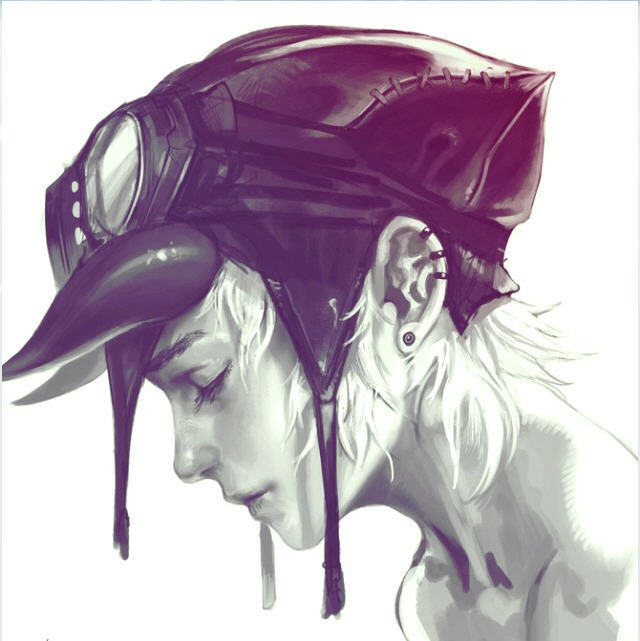
\includegraphics[width=0.3\textwidth]{logo.png} \\ % 放置你的logo 
  \vspace*{0.5cm}
  \small{\href{https://hivan.me}{茶桁}} \\
  \vspace*{1cm}
  \small{仓库地址: \href{https://github.com/hivandu/AI_Cheats}{Github}, \href{https://gitee.com/hivandu/ai_cheats}{Gitee}} \\
  \vspace*{0.2cm}
  \small{Email: feedback@hivan.me} \\
  \vspace*{0.2cm}
  \small{wechat: hivandu} \\
  \vspace{1cm}
  \vfill
  \hfill % 出版商logo右对齐
  \begin{minipage}[h]{0.2\textwidth}%
    \centering
    \small{坍缩的奇点@茶桁} \\
    \vspace{0.2em}
    
\includegraphics[width=\textwidth]{publisher.png} \\ % 出版商logo
    \vspace{1em}
    \small\today % 日期 
  \end{minipage}
\end{titlepage}

\setlength{\parindent}{2em}
\setlength{\parskip}{2ex}

% 设置图像label点击定位偏移量
\captionsetup[figure]{position=b}

\chapter{Introduction 简介}
\begin{figure}[ht]
  \centering\includegraphics[width=1\linewidth]{asset/茶桁的 AI 秘籍_数学篇.png}
\end{figure}

\newpage
\section{导言}

Hi, 大家好。我是茶桁。

在\href{https://mp.weixin.qq.com/mp/appmsgalbum?__biz=MzA4NzE4MDQzMg==&action=getalbum&album_id=3035995870421073928&scene=173&subscene=&sessionid=undefined&enterid=0&from_msgid=2648748542&from_itemidx=1&count=3&nolastread=1#wechat_redirect}{Python 篇} \href{https://mp.weixin.qq.com/s/mbnag65xDP-1Ct_81Byn5g}{PDF 发布}后, 我又制作了\href{https://mp.weixin.qq.com/mp/appmsgalbum?__biz=MzA4NzE4MDQzMg==&action=getalbum&album_id=3074770001140400130&from_itemidx=1&from_msgid=2648748768#wechat_redirect}{数学篇}。
  
在整个连载的过程中, 后台有小伙伴留言说想要电子书, 在公众号内进行阅读还是有些不太方便。在平时, 茶桁其实很多的知识和内容都是来自于公众号, 当然, 更多的是来自于书本。

咱们整个数学篇基本上都属于基础理论知识, 概念、公式、推导比较多, 但是为了让大家将数学概念和程序关联上, 在其中也涉及到了一些编码的部分, 也讲解了人工智能上数学是怎么应用的, 比如在 Chapter6 中, 我就给大家讲解了\hypertarget{数学如何运用于 AI}{数学如何运用于 AI}.

所有在数学篇内涉及到的程序代码, 也都在代码仓库中可以找到: 可以选择一个自己访问顺畅的进行拉取。

\begin{itemize}
  \item \href{https://github.com/hivandu/AI_Cheats}{Github}
  \item \href{https://gitee.com/hivandu/ai_cheats}{Gitee}
\end{itemize}

这个仓库内包含了目前为止整个《AI 秘籍》的全部代码以及数据集, 方便小伙伴下来之后进行练习。那仓库中的代码截至运行时间是 2023 年 12 月 26 日, 为什么要写这个, 因为有些包里的一些参数会做一些变动, 到目前为止这些代码都可正常运行, 假如过若干时间之后大家发现代码运行不了, 可以去看看包的官方文档, 也可以后台留言给我进行说明, 我会对电子书进行更新。

由于「数学篇」是一个付费专辑, 所以这本电子书并不是免费发放的, 仅针对已经付费的用户发送, 其余小伙伴想要阅读, 只能是进行购买了。不过本电子书是长期修正更新的, 在购买之后, 如果电子书内容进行了刊正, 则会对其进行更新, 并再次发送给已经购买的用户。还望小伙伴们在观看的过程中能够指出我的错误, 以便我对本电子书进行维护。

和制作 Python 篇的电子书的时候不同, 为了对数学篇进行付费的小伙伴们负责, 这次整个数学篇的电子书都一篇一篇进行了修正, 有些篇章更是重新写了一遍. 然后用 Latex 来重新设计和制作排版, 等于是整本书基本上都重构了一遍.

在修正的过程中才发现, 之前很多地方都有错误,有些错误甚至都是有误导性的. 在此要跟已经购买过数学篇的小伙伴们说声抱歉. 

当然, 虽然已经尽力的去寻找并且修正, 但也许不可避免的仍然还会有些错漏的地方, 在整个重新制作的过程中, 主要将经历放在了公式和概念上, 首先是争取对同学们不造成误导, 其次是有些地方的推导重新推导了, 争取能更容易进行理解. 在阅读过程中, 如果有小伙伴发现了错误或者遗漏, 还望给我留言, 我会尽快修正.

本电子书加入了版本号, 在每一章节的右下角部分, 如果有更新, 版本号都会有所变化. 并且在首页二维码下方的日期也会变化.

本电子书在\href{https://github.com/hivandu/Ebook_AI_Math}{Github 上公开了源码}, 不过由于内容还是付费内容, 所其中章节并未上传, 仅上传了主文件和一些设置内容. 不过对于想研究电子书制作的的小伙伴已经足够了.

最后, 感谢大家的支持, 特别感谢付费支持的小伙伴们。还望关注「坍缩的奇点」, 日后咱们会有一些干货分享给大家, 也会和大家一起来完成一些企业项目, 帮助小伙伴们更快的步入到实际工作中去。

\begin{figure}[ht]
  \centering
  
\includegraphics[width=0.6\linewidth]{asset/Capture-2023-11-02-164446.png}
  \caption{敬请关注「坍缩的奇点」,获取更多人工智能相关教程及资料。}
  \label{fig:img1_1}
\end{figure}
% \chapter{数学导论 - 概述}

\begin{figure}[ht]
  \centering\includegraphics[width=1\textwidth]{asset/茶桁的 AI 秘籍_Math_1.png}
\end{figure}

\newpage
\begin{quotation}
  因为 PDF 展示动图不方便, 当本电子书涉及到 gif 动图的时候, 并未直接展示而是给到了连接, 还望见谅. 
\end{quotation}

\section{前言}

大家好, 我是茶桁. 

在之前的一个多月前, 我有了写一个 AI 系列的想法, 起名为《茶桁的 AI 秘籍》, 简单规划之后, 于 7 月 27 日发出预告, 然后历时二十多天将近一个月\footnote{按本文完成时间而非电子书时间, 具体可以前往公众号「坍缩的奇点」查看. }, 完成了其中《Python 篇》的写作.  

不知道其中的内容对大家是否有帮助呢?

那么今天我又回来了, 根据规划, Python 以及相关第三方科学计算库只是我们基础工作的一小部分, 而很大一部分基础工作都还未进行. 

那么这次, 我依然给大家带来的是基础部分, 让我们进入 \href{https://mp.weixin.qq.com/mp/appmsgalbum?__biz=MzA4NzE4MDQzMg==&action=getalbum&album_id=3074770001140400130&from_itemidx=1&from_msgid=2648748768#wechat_redirect}{《茶桁的 AI 秘籍 - 数学篇》}. 

本节课的内容是「数学篇」的第一节课. 本节是一个导论. 我会为大家介绍一下这门课一些理论, 还有微积分、线性代数、概率统计里面一些比较基础, 和 AI 结合非常紧密的一部分, 难度并不会很大. 

觉得自己数学能力还不错的, 第一节课可以不用看, 直接去看后面的课程. 第一节课, 我们放松一点. 这节课难度真的不会特别的大, 主要是带大家了解一些比较有趣味性以及 AI 方面一些基础性的数学知识. 

数学对于计算机编程来说重要性是毋庸置疑的, 更何况我们现在不仅仅是编程, 而是走在「人工智能」的路上. 可以说, 数学应该是最重要的基础. 那从本节课开始, 就让我们进入「人工智能的数学基础课」. 

我们在学习 AI 的过程当中可能会遇到的一些关于数学方面的一些东西, 比如说线性代数里面的这个矩阵运算, 比如说这个求导, 还有一些概率统计, 图论方面的一些东西. 

如果您觉得自己对于微积分, 线性代数, 概率统计这些内容自认为掌握的还不错的同学, 其实是可以不用看了. 如果大家是从文科转过来或者说以前上的数学很多年了也忘的差不多了, 那可以来听听这些课. 

本节课的内容是「数学篇」的第一节课. 本节是一个导论. 我会为大家介绍一下这门课一些理论, 还有微积分、线性代数、概率统计里面一些比较基础、和 AI 结合非常紧密的一部分, 难度并不会很大. 觉得自己数学能力还是不错的, 这第一节课呢可以不用看, 可以直接去看后面的课程. 第一节课, 我们放松一点. 这节课难度真的不会特别的大, 主要是带大家了解一些比较有趣味性以及 AI 方面一些基础性的数学知识. 

首先我们会说一下为什么需要数学、人类从历史到现在是怎么表示数字的、计算机是怎么样对数字进行处理的, 还有我们也会说到计算机其实并不是像我们想象的那样无所不能, 它其实也有很多的漏洞. 然后接下来这几个模块我们就会分别去介绍微积分的基础, 主要是导数以及矩阵, 还有随机变量、图论里面这个图的概念. 

\section{为什么需要数学}

这个问题在古代有一个很明确的答案, 就是不管你是要丈量土地, 还是说要建立这种大型的水利工程, 或者说其他的工程项目, 你都不可避免的需要做很精确的这种数学计算. 

比如说古代皇宫他的新建, 或者说帝王这个陵墓的新建, 他都是需要一些非常精确的这种计算的, 包括从风水的角度. 而且大家都知道, 我们国家天文立法的水平其实是非常高的, 这也来源于我们在古代就建立起一套非常严密的数学体系. 

还有一个和生活比较贴切的例子就是算盘. 算盘不光是帐房先生用, 其实在古代用的面非常广, 我们知道就是现在有一门速算的这种能力叫做「珠心算」, 珠心算其实就是通过让学员在这个珠算上面去进行大量的训练. 训练到他们可以在自己的心里面去模拟出这么一个算盘出来, 然后他们就可以在心里面打这副算盘, 达到珠算的一个速度. 

\begin{figure}[ht]
  \centering
  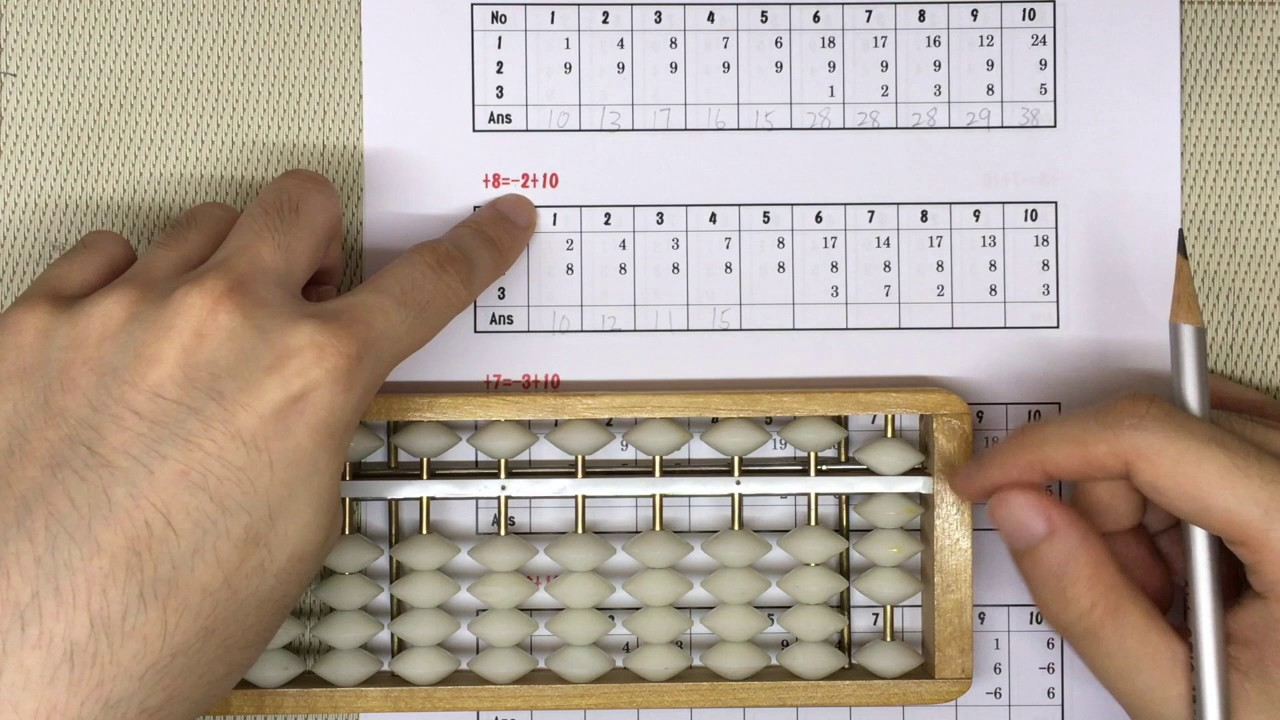
\includegraphics[width=0.5\textwidth]{asset/1c84c0f7-5335-4252-88ac-5e08192d89c3.png}
  \caption{}
  \label{fig:img2_1}
\end{figure}

那现代为什么我们需要数学呢?

大家可能会想到的就是因为高考得考对吧?大家都得拿着这个敲门砖去考大学, 然后将来进入社会. 

这个确实是一个, 不光是我们这门 AI 课程所需要涉及到, 在其他的一些科技领域, 比如说芯片制造、航空工程, 包括化工其实都是需要大量的数学. 

同样的, 在我们的商业活动当中也是可以见到数学的影子. 比如说大家知道量化金融分析、量化交易, 这个也是需要数学的, 需要大量数学计算. 而有一点大家可能想不到, 就是政治学其实也是需要数学的. 在西方的政治学其实是作为一个类似于自然科学的东西被研究的, 它那上面有非常详细的政治选举策略之类的内容, 甚至还融合了博弈论这些东西. 

\begin{figure}[ht]
  \centering
  
\includegraphics[width=0.5\textwidth]{asset/7e4f1c0f-936f-4b29-82e1-5294232218f3.png}
  \caption{}
  \label{fig:img2_2}
\end{figure}

\section{人类如何表示数字}

我们来说一下史前文明时期人类是怎么表示数字的. 

其实在地球的不同地区, 不管是在中国还是在外国都非常不约而同的出现\textbf{结绳记事}的方法. 

(图:\ref{fig:img2_3})是中美洲的一个印加文明, 它用来表示数字以及一些事物的. 这个方法就是在这个绳子上面打结. 

\begin{figure}[ht]
  \centering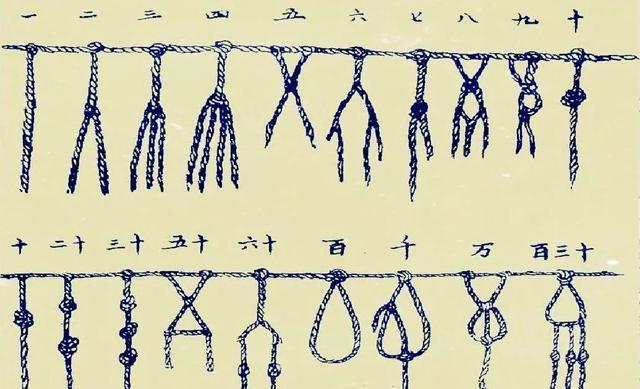
\includegraphics[width=0.5\textwidth]{asset/73a095be-4ca9-4065-abb0-5d919706b1dd.png}
  \caption{}
  \label{fig:img2_3}
\end{figure}

非常惊奇的是咱们中国古代也有类似的这种体系(图:\ref{fig:img2_4}). 

\begin{figure}[ht]
  \centering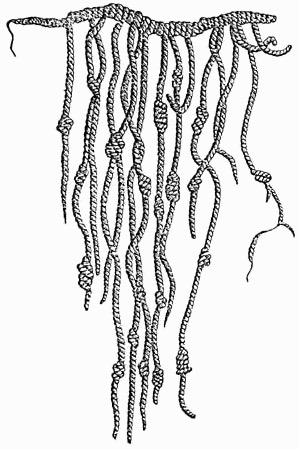
\includegraphics[width=0.4\textwidth]{asset/840839db-800f-44f2-8f4a-b7e17b896222.png}
  \caption{}
  \label{fig:img2_4}
\end{figure}

我们可以看到这上面不同的结对应的不同的数字. 这就是古人的一种基数体系. 然后等到文明在进一步发展了之后, 我们可以看到四大文明古国都发出了自己各自的文字符号体系. 

图:\ref{fig:img2_5}是古巴比伦人的楔形文字. 为什么叫楔形文字?这个楔在汉语里面的意思呢就是钉子. 为什么这种文字是这种楔形的呢?是因为它们是把这个竹片或者刀片在这种还没有干的泥板上面去刻字, 而刻出来的就是这种坑洼的形状. 

\begin{figure}[ht]
  \centering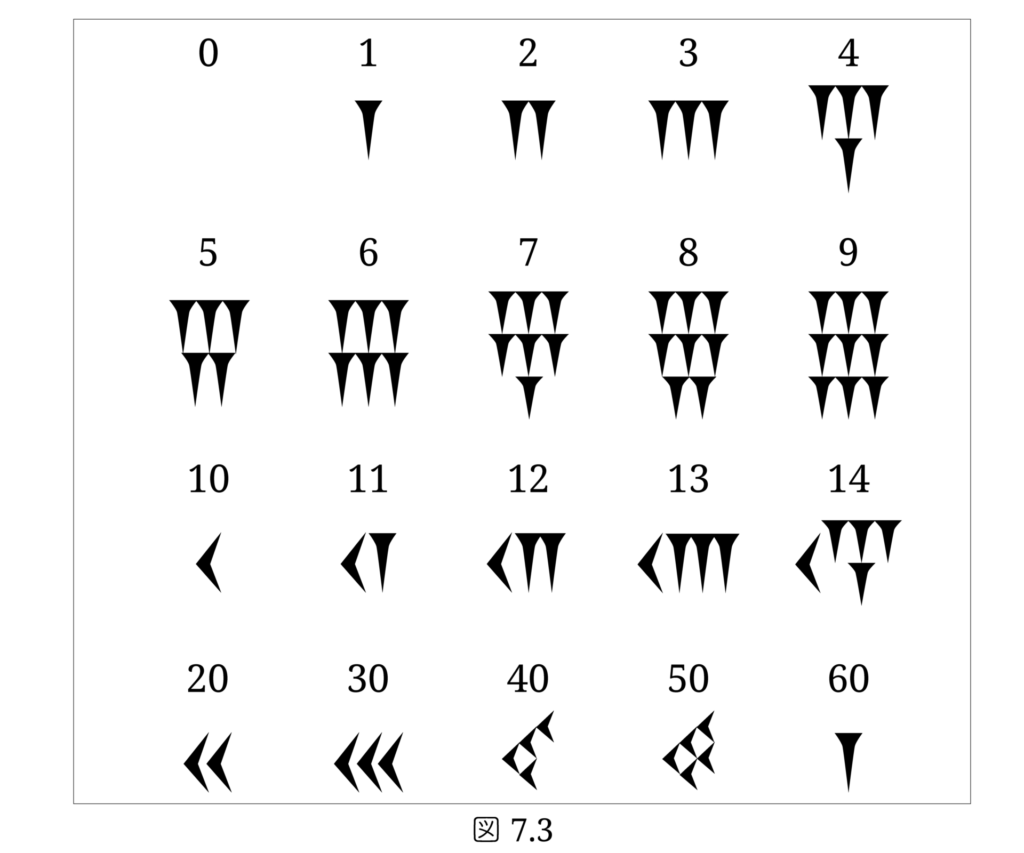
\includegraphics[width=0.5\textwidth]{asset/df03e920-b04e-493d-aab6-b5ffb16eb0bf.png}
  \caption{}
  \label{fig:img2_5}
\end{figure}

图 \ref{fig:img2_6} 是古埃及人的象形文字. 他们这个数字体系非常有特色, 融合了宗教的因素在里面. 比如说这个 1,000, 他是用一个睡莲的图案来表示, 手指呢代表了 1 万, 青蛙代表了 10 万, 天神呢代表了 100 万. 

\begin{figure}[ht]
  \centering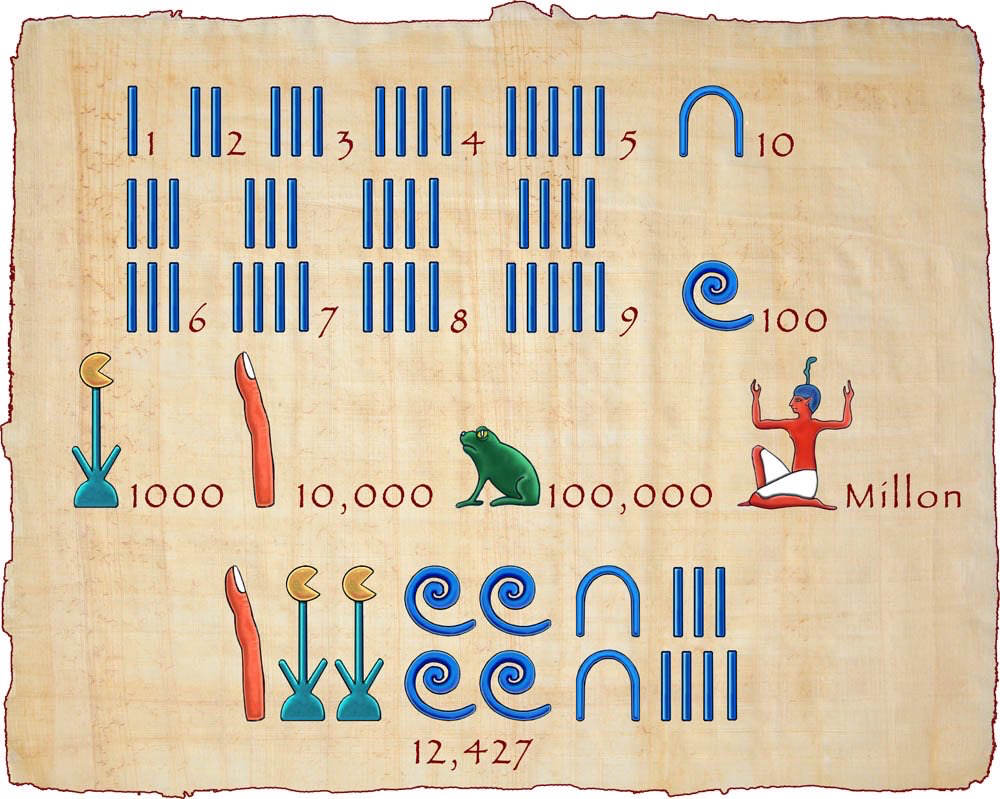
\includegraphics[width=0.5\textwidth]{asset/191cd6bc-63e3-4090-af11-bf3e7de6f4db.png}
  \caption{}
  \label{fig:img2_6}
\end{figure}

接着就是我们国家的(图:\ref{fig:img2_7}). 中国在甲骨文时代的文字技术体系还是有很明显的这种象形文字影子在里面, 尤其是像这个 1 万、3 万, 在我们看来可能现在像蝎子一样. 

\begin{figure}[ht]
  \centering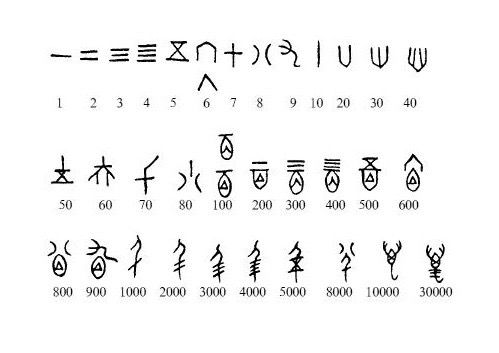
\includegraphics[width=0.6\textwidth]{asset/56174953-293d-47aa-893c-52ab80acacd9.png}
  \caption{}
  \label{fig:img2_7}
\end{figure}

然后就是古印度的数字体系(图: \ref{fig:img2_8}). 古印度有一点比较特殊. 我们知道其实阿拉伯数字不是阿拉伯人发明的, 这一点可能大家都知道, 这个是古印度人发明的, 只不过是由阿拉伯商人传到了欧洲, 所以欧洲人就把它称为阿拉伯数字. 虽然和我们现在使用的阿拉伯数字不太一样, 但是他有一些非常重要的概念已经被提出了. 比如说古印度人已经有这个 0 的概念了, 而且他有这个进位的概念. 什么叫进位呢?你看, 我们在其他的文明这个字符体系里面, 比如说这个 10, 它是用一个特别的符号来表示的, 但是在古印度的数字符号体系里面是用了一个一和一个 0, 这个 0 占一位来表示这个 10. 这点在我们现代人看来其实好像没有什么可说的, 大家可能会觉得不应该就是这样吗. 但其实这个在古代是一个非常了不起的一个成就. 

\begin{figure}[ht]
  \centering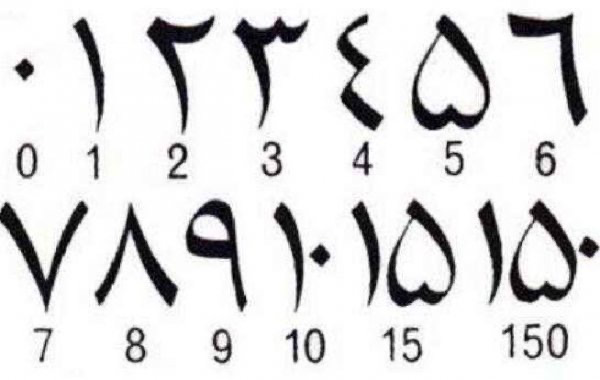
\includegraphics[width=0.4\textwidth]{asset/02cf4930-6fd5-40ab-b755-155d4bcf1fa1.png}
  \caption{}
  \label{fig:img2_8}
\end{figure}

同样的有一个文明需要说一下, 就是古玛雅文明. 古玛雅文明为什么放在这里说, 是因为他也提出了零和进位的这种概念. 他这个数字体系有两种, 一种呢是那种点横线的体系, 还有一种呢是和宗教息息相关的用神之的头像去表示数字的这种体系. 而他这个零和进位概念的提出比印度人和其他的古文明甚至还要早了将近一两千年. 所以这一点是非常了不起的, 很多这个科学家还有考古学家都觉得这个玛雅文明是一个外星文明的后代, 不然他不可能在其他四大文明古国之前一两千年就有了零和进位的这个概念. 

\begin{figure}[ht]
  \centering
  \begin{minipage}[t]{0.4\textwidth}
    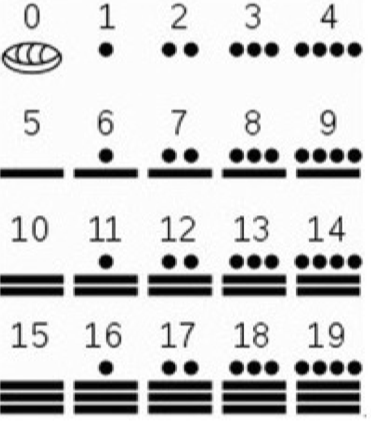
\includegraphics[width=\textwidth]{asset/265551e1-4fa0-4611-b795-3835b8967cf0.png}
    \caption{}
    \label{fig:img2_9}
  \end{minipage}%
  \hspace{1em}
  \begin{minipage}[t]{0.4\textwidth}
    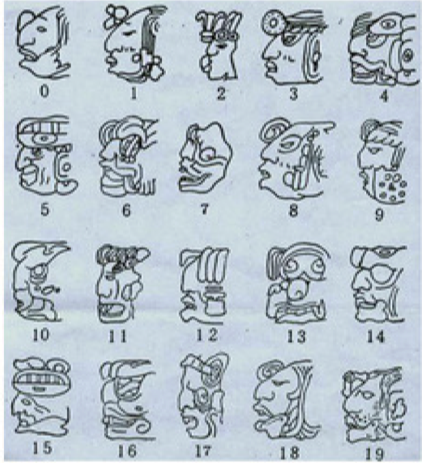
\includegraphics[width=\textwidth]{asset/71bac7f0-1042-47b2-a771-34b5eb04b656.png}
    \caption{}
    \label{fig:img2_10}
  \end{minipage}
\end{figure}

零我们会经常遇到它, 但是它不光是表示没有, 还表示着占位. 就比如说在进位里面它这个 0 如果在个位就表示占着个位, 然后如果这里再来个 1 它就表示 0 前面的 1 表示 10, 这是一个非常重要的概念. 

\section{计算机可以做什么?}

\begin{figure}[ht]
  \centering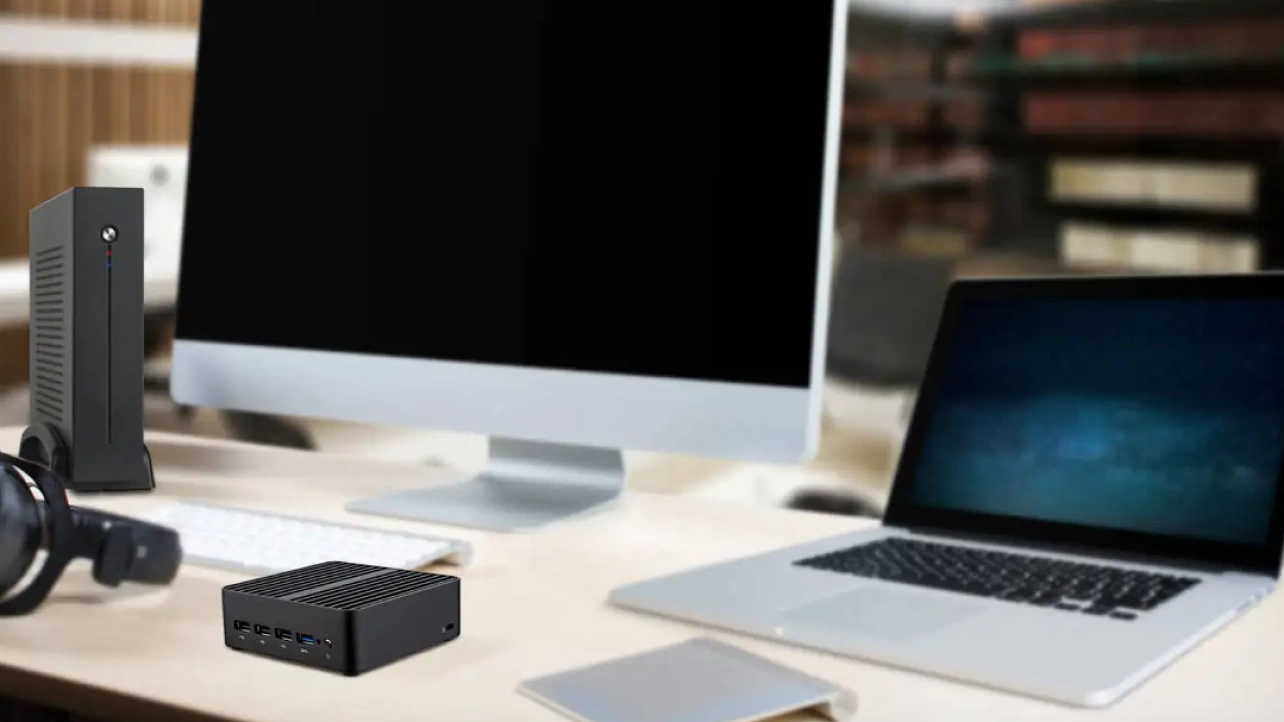
\includegraphics[width=0.8\textwidth]{asset/7b8b9bd7-b7db-4420-bcce-537d0be46a31.png}
  \caption{}
  \label{fig:img2_11}
\end{figure}

这个用途就太多了对吧, 像这个烟花一样, 散发到空中然后太多太多了. 

比如说我们可以用计算机去做图像处理. 说简单一点话就是 PS 或者说美颜, 我们可以对这个音频信号进行一个处理, 大家用这个百度啊或者高德导航啊能听到各种名人的这个声音, 其实那个真的是让名人说那么多的话吗》不是的, 其实可能也就是让那些人说个一两句两三句然后就根据他们这个声信号去合成, 用他们的发音特征, 而说出来这种这种语音. 很神奇对不对?

然后还有比较常见的:word、PPT、Excel 这种字处理软件都是用计算机可以去做的. 包括我们有一些做科研的同学应该很清楚, 很多科学建模这种模拟也是用计算机去做的. 很多东西我们没办法在现有的实验室条件下去做, 或者经费太贵了导师给不起, 所以这个我们也用计算机去做. 当然还有大家最感兴趣的就是游戏. 

那计算机他是怎么样做到的呢?

其实, 不管你是哪一种类型的数据:不管是图像也好、音频信号也好、还是处理文字、还是说科学计算游戏等等, 其实在计算机看来呢都是一样的. 在计算机看来呢它都是$0101$这种字符, 都是数据流. 在计算机看来是分不清什么是游戏、什么是图像、什么是音频. 不管哪一种类型的数据它都是$0101$这种数据流. 

那计算机如何去处理这个$0101$就很重要了. 

首先我们先来了解一下:这个$01$它是怎么样去做运算的. 

其实$01$二进制的运算和我们这个十进制的加减乘除没有什么区别, 可能最大的区别就是十进制它有$0123456789$这十个数字
来表示所有的数字, 而在二进制里面它只有$0$和$1$两个字符来表示所有的数字. 二进制里面$1+1$不是说等于 2 了, 它就是是$10$(不是十, 是一零), 2 只是在十进制里面. \ref{tab:table2_1}

\begin{table}[ht]
  \centering
  \begin{tabular}{ll}
    \toprule
    二进制加减法则  & 二进制乘除法则 \\
    \midrule
    $0+0=0$ & $0 \times 0=0$ \\
    $1+0=1$ & $1 \times  0=0$  \\
    $0+1=1$ & $0 \times  1=0$  \\
    $1+1=10$  & $1 \times  1=1$  \\
    $0-0=0$ & $0 \div 1=0 $ \\
    $1-0=1$ & $1 \div 1=1$  \\
    $1-1=0$ & \\
    $10 - 1=1$ &  \\
    \bottomrule
  \end{tabular}
  \caption{ 二进制运算法则}
  \label{tab:table2_1}
\end{table}

接下来我来给大家说一下二进制和十进制的转换. 其实也很简单, 有小学基础就可以, 主要我们要搞清楚这二进制的数字它是表示着什么东西. 

我们知道对于一个十进制数而言它的百位上面数字, 比如我说一个数字 345, 那它百位上面数字 3 就代表它有 3 个 100, 十位上的 4 就代表 4 个十, 个位上的 5 就表示 5 个一, 所以十进制数的 345 是怎么样去计算的?他就是 3 乘以 100 再加上 4 乘以 10 再加上 5 乘以 1, 结果就是十进制里面的 345. 

同样的对二进制而言也是一样, 只不过二进制的底不一样, 它不是十进制里面的 10. 咱们就把十进制里面这个 10 或者 100 给它换成 2 的零次方, 2 的一次方, 2 的二次方就行了. 

\begin{figure}[ht]
  \centering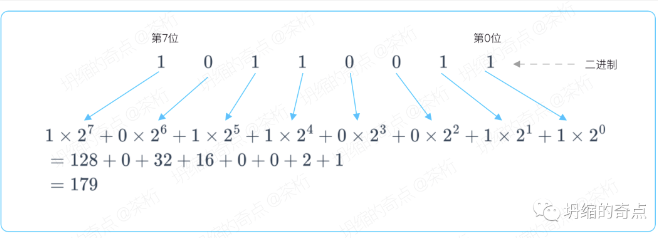
\includegraphics[width=0.8\textwidth]{asset/20231227140607.png}
  \caption{}
  \label{fig:img2_12}
\end{figure}

比如说图 \ref{fig:img2_12} 最右边一位就是二进制的个位数, 二进制的个位数它就代表了 2 的 0 次方. 其实我们想一下很容易理解, 我们刚才说到 345 里面这个 5 是 5 乘以 1 得来的, 那这个 1 是怎么得来呢?1 其实是 10 的 0 次方. 就是说这个是任何数除了 0 之外 0 次方都等于 1. 二进制的十位数是 2 的一次方, 依此类推次数都会一直递增, 递增之后我们把前面的数值和这一位代表的位数相乘在一起. 把它所有结果相加就是十进制的数. 也就是:

\[
  1\times2^7+0\times2^6+1\times2^5+1\times2^4+0\times2^3+0\times2^2+1\times2^1+1\times2^0=179
\]

反过来,十进制的数怎么转成二进制呢? 这个你可以把它理解为不断除 2 取余法. 我们把这个数不断的去除以 2, 与此同时得到余数, 一直这样除下去到什么时候为止呢?一直到被除数的商等于 0. 现在我们得到了一连串的余数, 从下往上的顺序把它排列成这个二进之数, 如图 \ref{fig:img2_13}, 也就是$11010111$这个二进制数. 

\begin{figure}[ht]
  \centering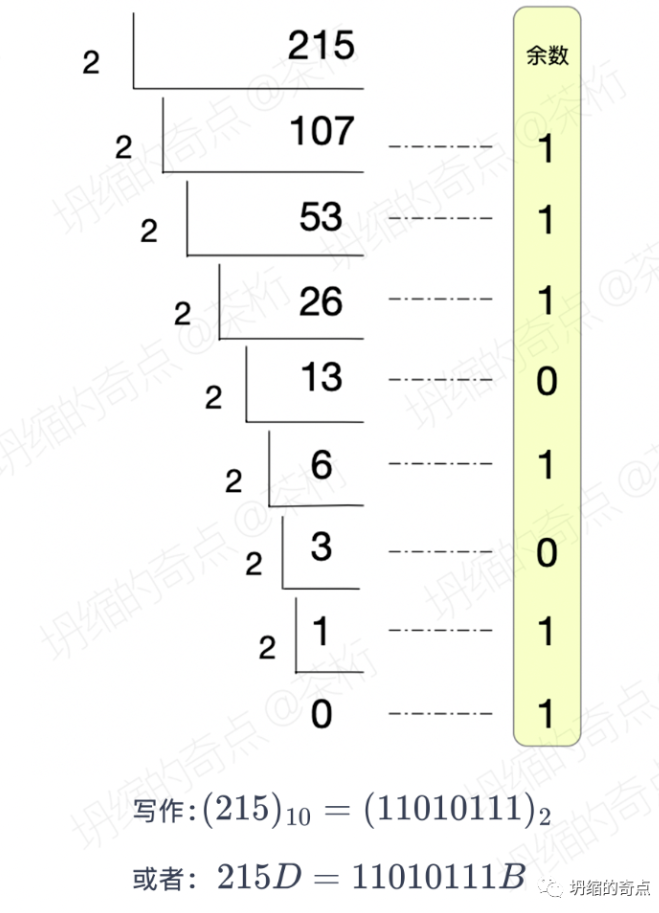
\includegraphics[width=0.4\textwidth]{asset/20231227140715.png}
  \caption{}
  \label{fig:img2_13}
\end{figure}

在第二种表示法中, D 就是 Decimer, 十进制的意思, B 是 Binary, 二进制的意思. 不难吧?

我们再说看看, 计算机是如何处理二进制数据的. 

之前我们讲过, 计算机无法处理十进制数, 所有的数据进入计算机都必须转成二进制的数据流. 那么大家是否会有疑问, 就是 $0101$ 这种数字, 计算机是怎么处理复杂的东西, 比如说游戏什么的. 

我来给大家看一张逻辑电路图(\ref{fig:img2_14}):

\begin{figure}[ht]
  \centering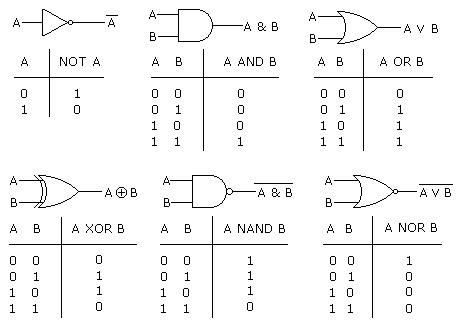
\includegraphics[width=0.5\textwidth]{asset/975a7883-49a7-4b15-8102-0352aebc5568.png}
  \caption{}
  \label{fig:img2_14}
\end{figure}

最上面的三个, 就是所有计算机电路机构的基础, 不管再怎么复杂的电路或者芯片, 最终都是以这三个为基础构建出来的. 

第一个叫做非门, 简单理解就是这个门是一个对着干的门. 你给我一个 1, 我就给你个 0, 你给我个 0, 我就给你个 1. 
第二个叫与门, 这个也好理解, 就是两个条件都必须满足才行, 就是你必须语文 150 分, 数学也 150 分, 爸爸妈妈才会给你买最新的 iPhone 15 Pro. 那么这个门里, 我必须是两个条件都是 1, 最后才会输出 1, 否则都会输出 0.
第三个叫或门, 从字面上看都很好理解了是吧?就是你语文「或者」数学考 150 分了都可以, 都会带你去吃一顿大餐. 那么这个门, 我们只要传入一个 1 就可以了, 就会输出 1. 当然, 两个都是 1 的情况就是你两个都考了 150 分的情况, 当然更好对吧, 也会输出 1, 也就是会出去吃一顿大餐. 

不管再怎么复杂的电路再怎么精密复杂的计算机, 其实都是由这种简单的小部件不断的累积不断的重叠加在一起获得的. 

那么下面三个我们这里就不解释了, 也不是重点. 对计算机原理感兴趣的同学可以去看看下面这节课:

计算机也并非无所不能. 我们都遇到过计算机突然崩溃不行的时候, 俗称蓝屏或者四国对吧?又或者, 计算机遇到了黑客, 或者我们不小心电脑中毒了, 致使个人信息全部被窃取了. 那这个都是计算机漏洞导致的. 

再比如说我们程序员经常遇到的, 就是我们写了一个程序:$0.1+0.2$, 我们会认为应该运行结果就是$0.3$对吧?但是实际上的情况呢?我们来做个实验看看:

\begin{figure}[ht]
  \centering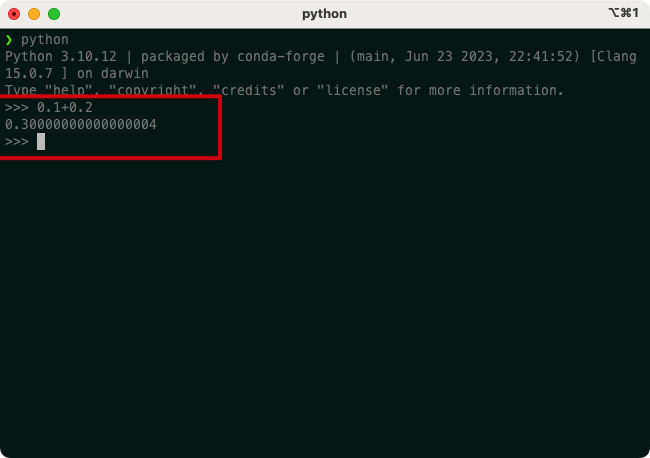
\includegraphics[width=0.6\textwidth]{asset/ef878802-961f-4168-9900-da12253d4b48.png}
  \caption{}
  \label{fig:img2_15}
\end{figure}

结果并没有如预期一样, 而是得到了一个意外的数字, 一大串的 0 后面跟了一个 4.

我们需要从二进制的原理去理解, 之前我们学到的内容是十进制的整数转二进制, 用的是除 2 取余法, 但是小数的十进制转二进制, 需要用的方法不太一样, 叫做乘 2 取整法. 如图 \ref{fig:img2_16}:

\begin{figure}[ht]
  \centering
  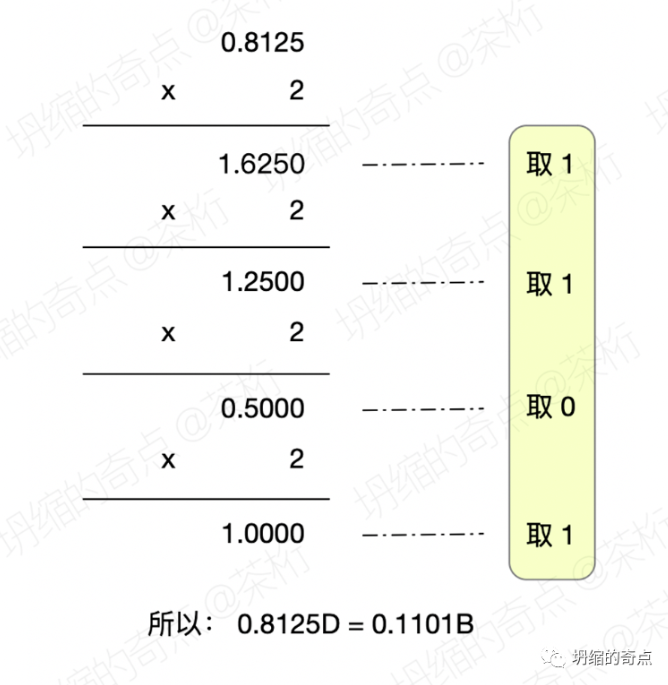
\includegraphics[width=0.4\textwidth]{asset/20231227140841.png}
  \caption{}
  \label{fig:img2_16}
\end{figure}

注意和整数的排序不同, 小数点后面的计算是从上往下顺序排列的. 

那二进制可以准确表示 0.1 吗? 我们按照刚才学的内容来算的话 就应该是 

\[0.000110011001100110011001100 ... \]

会无限循环下去. 

但是计算机内表示数字不可能无限循环下去, 是有限制的. 我们接着往下看:

\begin{figure}[ht]
  \centering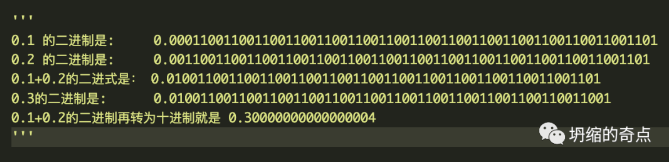
\includegraphics[width=0.8\textwidth]{asset/20231227140947.png}
  \caption{}
  \label{fig:img2_17}
\end{figure}

那为什么是这个位数呢?因为再循环下去也没有意义, 所以到保留到那一位之后就不往下取了. 我们也不用去数这些 0 和 1 到底是多少位, 知道是怎么回事就行. 我们看到第三行和第四行的表示并不一样, 这就是为什么我们计算$0.1+0.2$的时候并不会是$0.3$, 而是还跟着一串 0 接一个 4. 

那这个问题我们怎么解决呢?因为很多场所下我们都需要高精度的数字. 其实也很简单, 转成整数再计算就行了, 因为整数转二进制没有这种问题, 比如说$0.1+0.2$, 我们计算$1+2$, 然后再除以 10 就可以了. 

在一些要求不是很高的应用场景内, 我们可以提高可表达数的精确度就能满足需求. 比如\textit{big decimer},  在 Java 这些语言里面都有. 

然后我们再来思考一下, 这种问题是二进制里才有的吗?其实并不是, 比如我们十进制就经常有无限循环小数对吧?比如说 $\frac{1}{3}$,  如果写成小数的形式也是一样, 3 会无限循环下去. 所以这并不是二进制独有的问题, 所有的进制都会有这样的问题. 那么问题来了, $0.9999 ... $无限循环下去, 是否等于 1 呢?

其实答案为「相等」. 怎么证明呢?

我们说$1/3 = 0.333333 ... $,  那么$0.3333 ...  \times 3 = 0.9999 ... $,  等式右边乘以 3 了, 那左边也一样会乘以 3,  得到$1/3 \times 3 =1$. 所以最后我们可以得出结论, $0.9999 ... =1$对吧?

然后我们来看, 人工智能是如何运转的?

人工智能是利用计算机这种强大的算力, 按照 AI 模型的规则实现特定的逻辑推断任务. 简单点说就是以前人能进行的思考、逻辑推理推断的活动我们现在希望计算机也可以有. 

有的同学可能会问:那计算机现在没有吗?计算机其实是一种自动化的程序, 这种规则的制定都是按照我们事前已经约定好的规则. 它只能按照我们既定的规则去做, 超出了这个规则之外是没办法去做的. 比如说我这个程序只会负责把林志玲的声音合成然后输出, 那我想让它生成郭德纲的就不行. 超出了能力范围, 它也不知道怎么去弄. 

人工智能就是希望他能让计算机拥有自我的思维逻辑推理能力, 不管是哪一种 AI 模型, 无论是现在特别火的大语言模型, 机器学习里面的深度学习、神经网络、还是说什么朴素贝叶斯都是
高度依存于我们现有的这种数学体系. 所以, 人工智能和数学息息相关. 

不过大可放心, 难度没有太大. 不会像数学系那样, 还让你去求什么「一致连续」、「区间套定理」、「7 个定理循环证明」等等. 不可能是那样子的, 我们更多的是拿来用就行, 难度也不会特别的大. 

学习人工智能我们需要哪几个方面的知识呢?

主要是四个:1. 微积分;2. 线性代数; 3. 概率 \& 统计;4. 图论. 

相对来说, 前三个应用的会稍微偏多一点. 图论也会有一些应用, 比如说在一些图优化里面
或者网络搜寻会用到. 这四个内容我们都会接触到. 

好了, 之前铺垫了那么多. 那接下来就正式开启了数学基础的模式. 
% \chapter{数学导论 - 微积分基础:导数}

\begin{figure}[ht]
  \centering\includegraphics[width=1\textwidth]{asset/茶桁的 AI 秘籍_Math_2.png}
\end{figure}

\newpage

我们需要用几节课来对一些基础的数学内容进行一下回顾, 能回忆的起来的小伙伴非常优秀, 回忆不起来也没关系, 跟着我的节奏往后走就可以了. 

本节课, 我们先来回顾一下微积分的基础(导数). 

\section{函数}

首先, 我带大家回顾一下: \textbf{函数它是一个什么样的东西}. 

按照我们记忆或者说印象当中的, 函数是左边一个因变量 y(通常用 y 来表示), 右边是一个函数式子: $y=x+1$, 函数式里面包含了次变量. 

我们来看四张图:

\begin{figure}[ht]
  \centering
  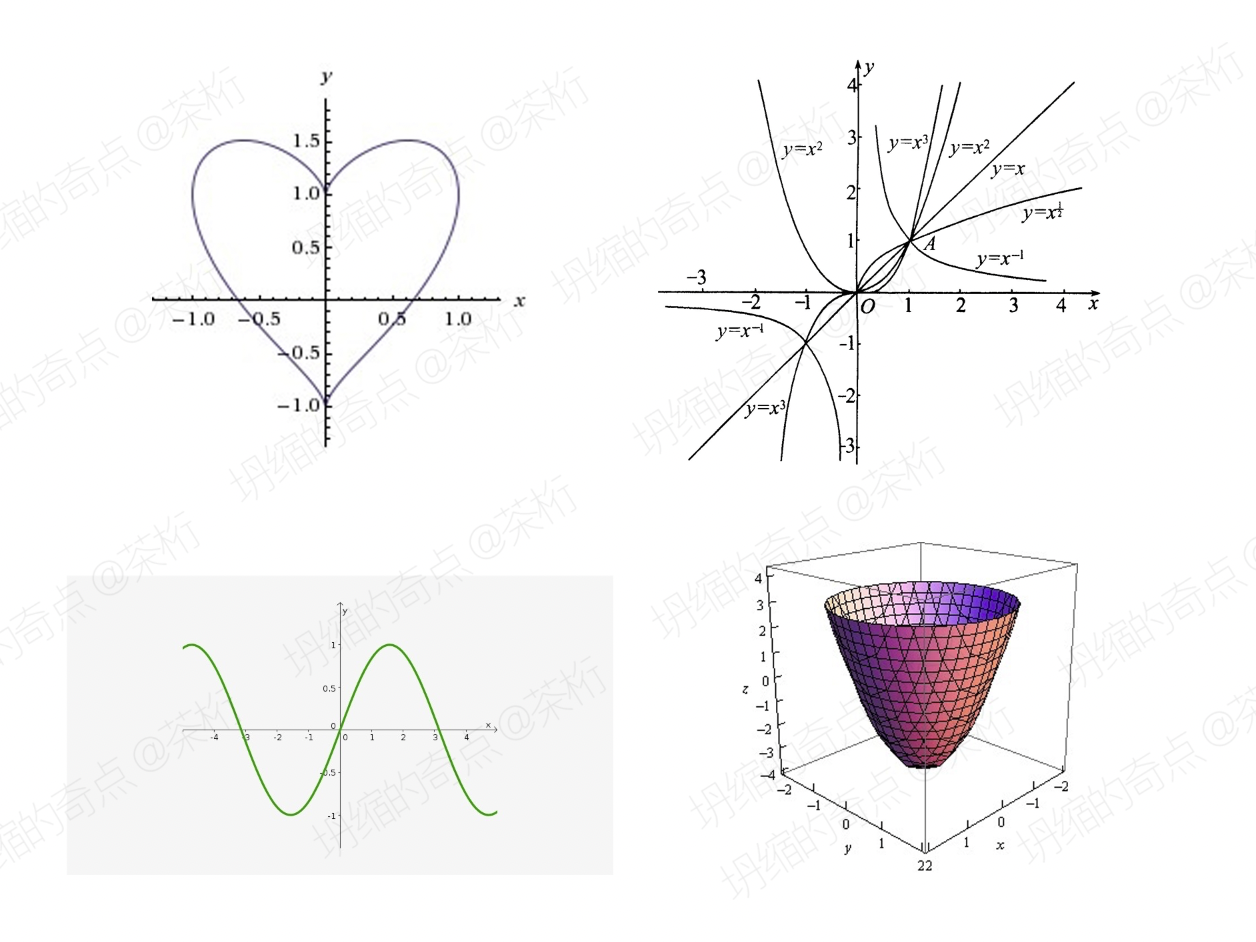
\includegraphics[width=1\textwidth]{asset/fa27e701-ba74-4406-bcb2-7956f4188918.png}
  \caption{多种函数的图形}
  \label{fig:img3_1}
\end{figure}

这些图像, 有的是函数, 有的不是函数. 大家知道这四个图像里面, 哪一个不代表着函数图像吗?

就是左上这个并不是函数. 因为什么呢? 因为它的一个 x 值对应着两个 y 值. 就比如说 $x=0$ 这个值, 在上方和下方各对应着两个 y 的值 $(1.0, -1.0)$. 这是不符合函数定义的. 那其他这几个呢, 都是函数的图像. 如果大家答对了, 我也就安心了, 说明大家对这部分还没有忘. 

函数的形式有很多种: 一次的、二次的、正旋、指数、对数、多元函数等等. 

\begin{align*}
    & y=x^2 & y=sinx \\
    & y=e^x & y={log_2}x \\
    & z=x^2+y^2 & ...
\end{align*}

如果我们抽象一点来看, 可以把函数理解成什么呢?就是我给它一个输入, 然后按照这个函数设定好的规则给我一个输出, 如图 \ref{fig:img3_2}. 

\begin{figure}[ht]
  \centering
  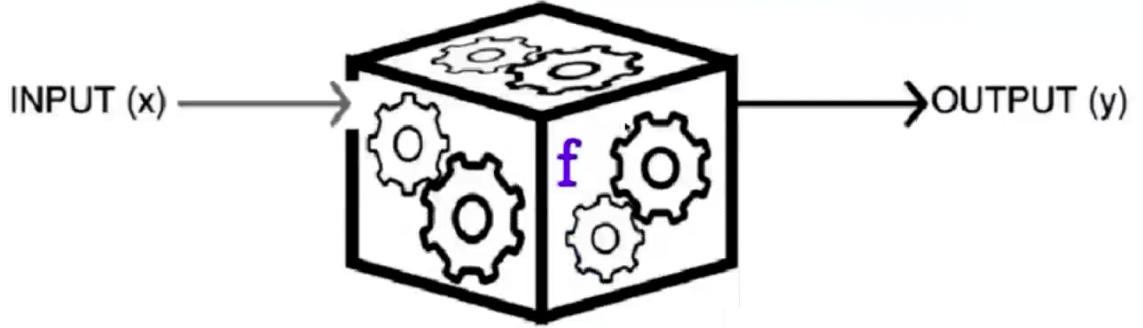
\includegraphics[width=0.5\textwidth]{asset/9f20645c-ef49-4ffd-9178-d01b67c74249.png}
  \caption{什么是函数}
  \label{fig:img3_2}
\end{figure}

拓展讲一下, 大家知道「函数」这个中文是怎么来的吗?\textbf{李善兰}是清代的一个数学家, 他那个时候看到 function 这个词就觉得不能音译过来, 不能跟日本人一样什么词都音译过来, 就是要取一个中文名. 函数就像一个黑盒子一样, 你不需要了解它内部的构造是什么, 你给它一个输入, 它就能按照规定的规则给你一个输出. 所以「函」代表着什么意思?代表的就是盒子包装起来. 比如「石函、剑函」, 基本字义就是「匣, 盒子」的意思. 

除此之外, 李善兰所创立的二次平方根的幂级数展开式, 研究的各种三角函数, 反三角函数和对数函数的幂级数展开式也成为了“十九世纪中国数学界最大成就”. 

李善兰把 function 这个词翻译成了函数,就表示这个规则是装在一个黑盒子里面一样. 更抽象一点, 自变量的数量是可以有很多种. 就是说函数的输入不一定非得是一个, 它有 n 多个. 你有 1,000 万个、100 万个都行. 但是它输出只有一个. 

\begin{align*}
    x,y,...(\mbox{自变量}) \Rightarrow f(\mbox{函数}) => z(\mbox{因变量})
\end{align*}

这个就叫做多元函数, 就是它的自变量如果超过一个叫做多元函数. 自变量只有一个叫做一元函数. 

\section{导数}

在简单回顾了函数之后, 我们来说一下导数. 

导数这个东西我们怎么样去理解呢?我们用一个运动学的例子带大家理解一下. 

首先我们来看一下图 \ref{fig:img3_3}, 这个坐标系可以看懂吧?这个平面直角坐标系中 x 轴代表这个自变量, 纵轴代表了因变量. 这个运动问题里面横轴(x 轴)就代表了时间, y 轴代表了位移. 运动问题:(y: 位移,  x: 时间).

\begin{figure}[ht]
  \centering
  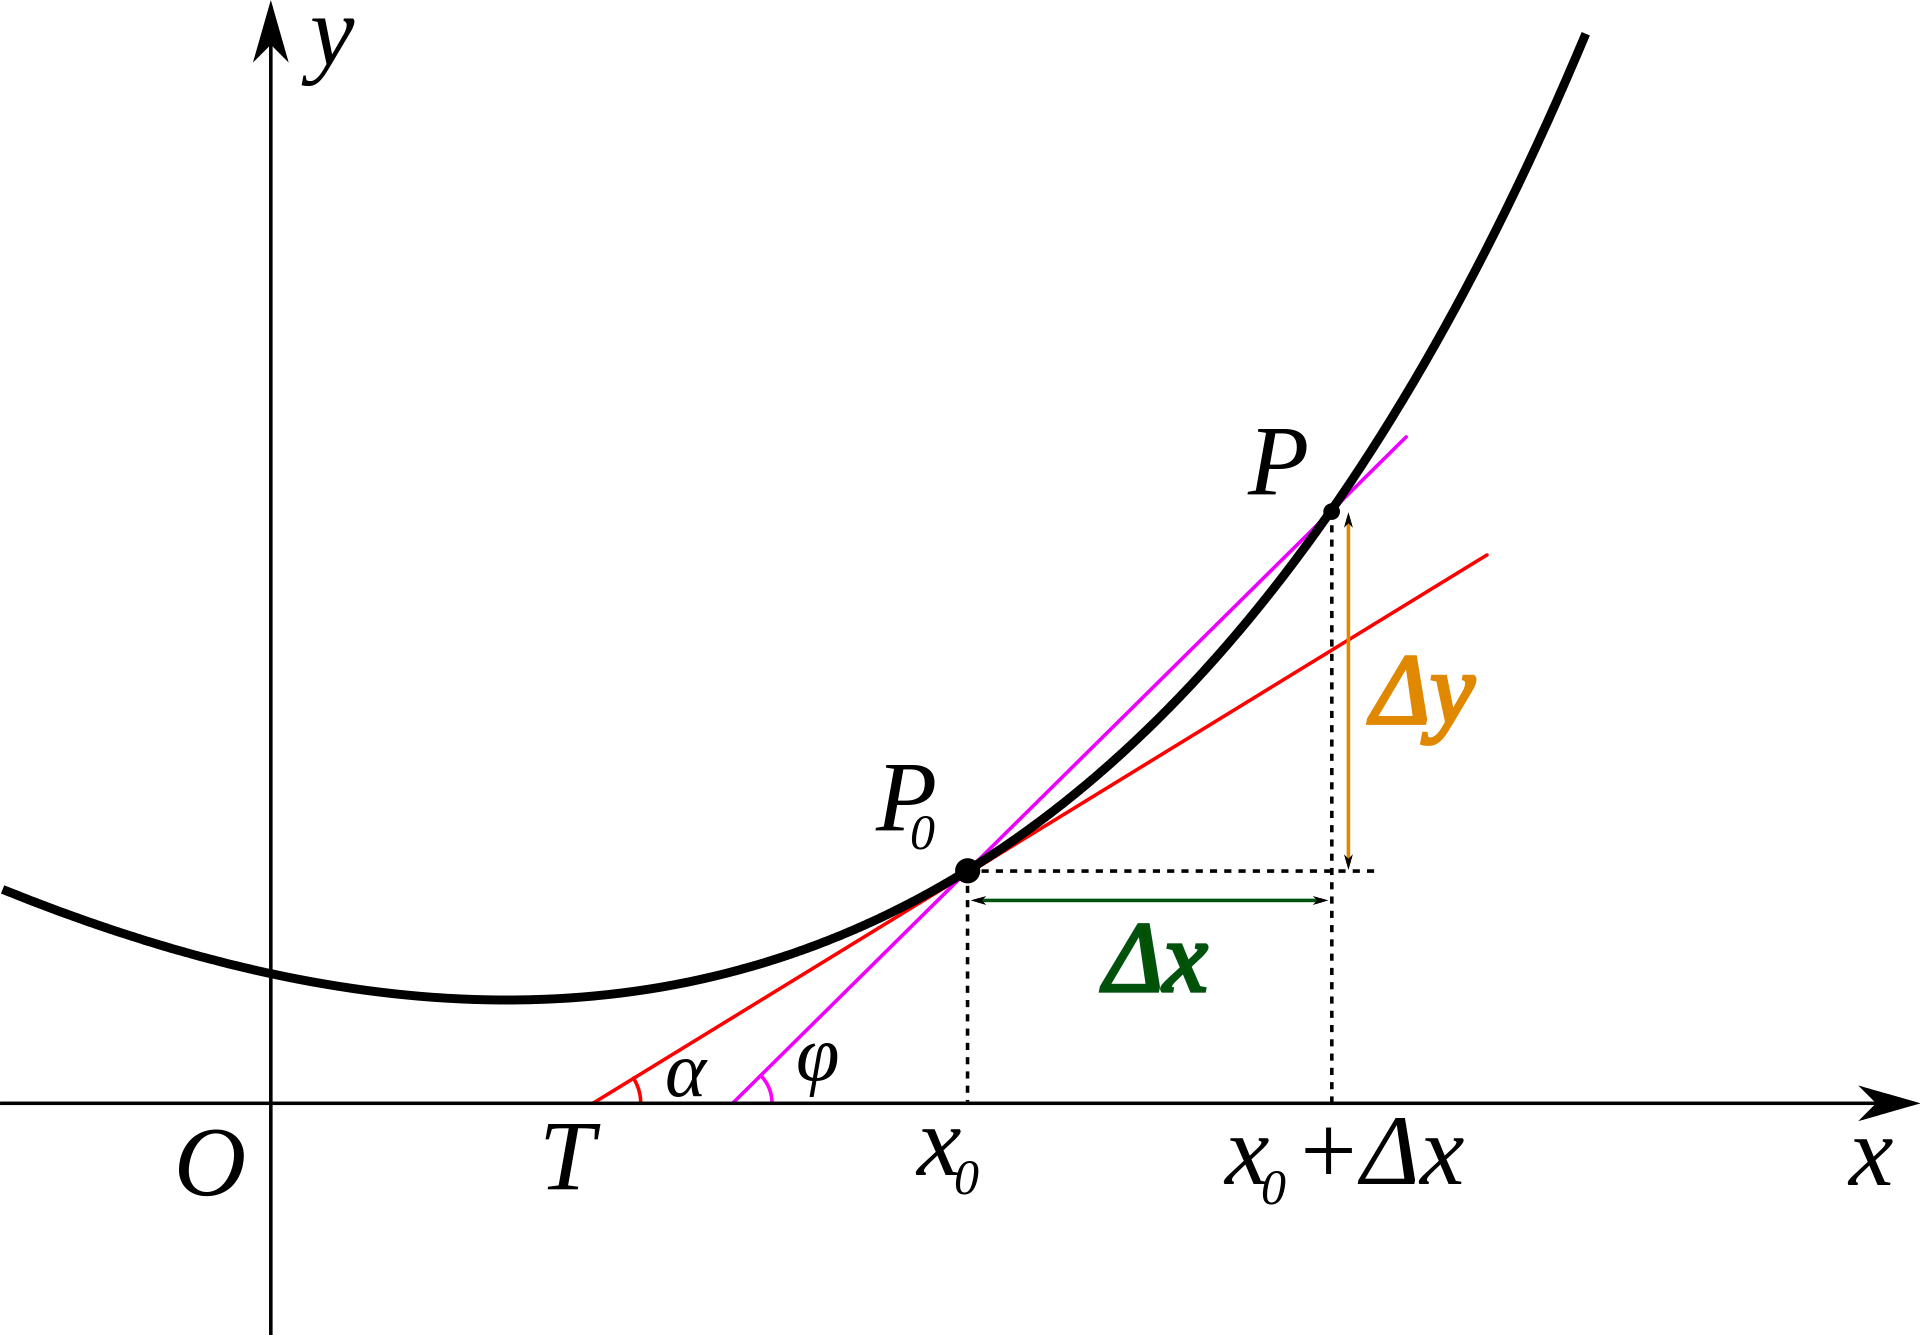
\includegraphics[width=0.7\textwidth]{asset/8b53b1a6-4a67-4402-b86a-b29dab8c535b.png}
  \caption{}
  \label{fig:img3_3}
\end{figure}


我们来看一下这个运动图像是这条黑线, 然后我们来考虑一下$P_0$和$P$这两点. 

如果我们只看这一段, 也就是质点从$P_0$运动到$P$这个位置, 那么它就位移了$\Delta y$, 一共花了$\Delta x$的时间. 我们就能得到$P_0$和$P$这一段运动的平均速度$\overline{v}=\frac{\Delta y}{\Delta x}$. 

在这个过程中, 我们不断的让$P$接近$P_0$,我们并不是说让质点移动, 而是在图像上的两点越来越接近的时候, $\Delta y$和$\Delta x$也在逐步的缩小,  逐步缩小到$P$几乎就要和$P_0$重合. 最终重合的时候, 本来$P$和$P_0$是形成了一条割线(紫色的直线), 当两个点融合为一个点的时候他就退化成了一个切线(红色的直线), 这个切线就是$\Delta x$趋向于 0. 在$P$无限接近$P_0$的时候, 我们就是在求$P_0$这个瞬时速度. 基于之前的分析, 那么我们就得到瞬时速度公式:

\begin{align*}
  \lim_{\Delta x\to0} \frac{\Delta y}{\Delta x}=\tan a
\end{align*}

我来解释一下这个公式, $\lim$ 表示取极限的意思, $\Delta x \to 0$表示$\Delta x$趋近于 0,  整个公式就是$\Delta x$趋近于 0 的时候$\frac{\Delta y}{\Delta x}$计算结果等于$\tan a$, 也就是正切值. 也就是$\angle \alpha$这个三角形中对边比上临边, 如图 \ref{fig:img3_4}:

\begin{figure}[ht]
  \centering
  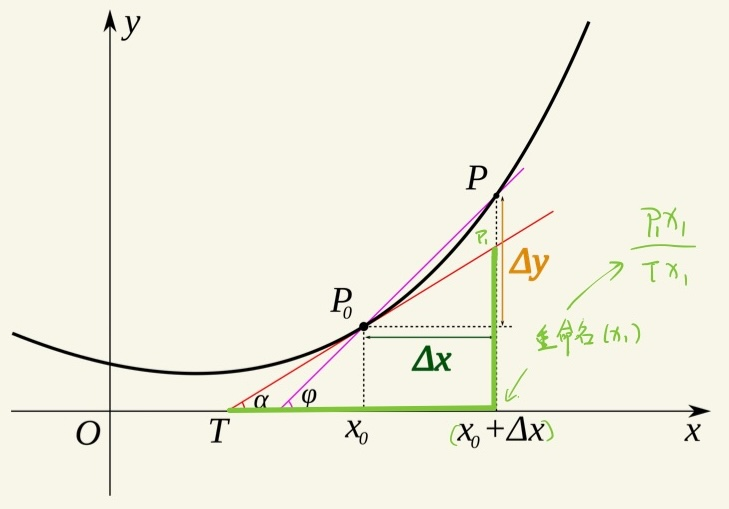
\includegraphics[width=0.8\textwidth]{asset/ac2df882-fb9f-4ddc-ae48-888ff4dec6a6.jpg}
  \caption{}
  \label{fig:img3_4}
\end{figure}

其实并不是说是我们如图看到的那两条线段就是$\Delta y$和$\Delta x$, 而是说他们代表的比例是相等的, 因为它们已经退化成了切线了, 所以我们只能用这个角度来表示. 

\section{导数与微分(一元函数)}

现在我们就可以引入导数正式的定义:

\begin{align*}
  y'=f'(x)=\lim_{h \to 0}\frac{f(x+h)-f(x)}{(x+h)-x}
\end{align*}

大家不用看到这个数学公式就非常紧张, 没必要. 从我学习的经验来看, 其实很多大白话能说清楚的事情, 非要起一个学术的名字, 非要用一个听不懂的概念来说. 其实当我们真正不被字符和符号来迷惑的时候, 就会觉得这些东西非常简单. 

那这个导数是什么意思呢?一般导数我们都会用 $'$ 来表示, 比如公式中的$y'$, $f'$, 它是相应函数的导数. 比如$f'(x)$就是表示$f(x)$的导数. 它的定义其实就是我们的趋近过程, 我们取两个点, 一个是$x+h$,  一个是$x$, 也就是图像中的 $x_0+\Delta x$ 和 $x_0$ 这两个点, 当$h$无限趋近于 0, 分子部分是函数$f(x+h)$ 和函数$f(x)$的差值(也就是图像中的$\Delta y$), 分母部分是$(x+h)-x$,就相当于图像中横坐标的差值, 也就是$\Delta x$. 那我们的导数的定义就出来了, 就是我们求图像的某一段, 其纵坐标的差比横坐标的差, 当两点距离越来越小的时候, 我们就得到其导数了. 也就是在图像中, 我们得到了$P_0$这个点上的切线的斜率. 

接着就是一些相关定义:

\begin{itemize}
  \item $y$被称作$y'$的原函数
  \item $y'$被称作$y$的导函数(导数)
  \item 微分:当自变量 x 的变化趋于无穷小时($dx$), 因变量 f(x)的变化情况($df(x)$). 
\end{itemize}

\begin{align*}
  df(x)=f'(x)dx
\end{align*}

微分的概念很多人容易和导数混淆, 它们的概念是有点相近, 但是代表的是不同的含义. 比如说在上面那个图像中, 质点从$P_0$点向$P$移动, 这个移动量几乎不可察觉, y 也就是一点点的变化. 不管移动了多少, 也就是相当于横轴上$x_0$向右移动一点点, 那这个图像也就向上移动了一点. 当自变量 x 增加或者减少了一点的时候, 因变量$f(x)$增加或者减少了多少. 这个自变量和因变量的变化量, 都用$d+\mbox{变量}$来表示. 这个$d$就是表示微分的意思. 那么$dx$就是 x 具体变化了多少量(当然这个量是非常小的, 可以想作趋向于 0), 与之对应的, $df(x)$也就是因变量$f(x)$具体变化了多少量. 

在神经网络中, 优化反向传播, 也就是反向传递这个导数的过程. 所以说, 导数还是一个很核心的一个概念. 

下面这个就是我们常见的一些函数的导数, 这些函数也就是一些初等基本函数. 

\begin{align*}
  & C'=0 & (x^n)'=nx^{n-1} \\
  & (sinx)'=cosx & (cosx)'=-sinx \\
  & (a^x)'=a^x \ln a & (e^x)'=e^x \\
  & (log_a{x})'=\frac{1}{x}log_a{e} & (\ln x)'=\frac{1}{x}
\end{align*}

来看一个求导的例子, 我们利用导数的定义求证一下其中一个函数导数: $(sinx)'=cosx$

\begin{align*}
  \mbox{求证}:&  (sinx)'=cosx \\
  \mbox{证明}:& \mbox{令}f(x)=sinx \\
  \mbox{因为}:& f'(x)=(sinx)' \\ 
  & =\lim_{h\to0}\frac{f(x+h)-f(x)}{(x+h)-x} \\
  & =\lim_{h\to0}\frac{sin(x+h) - sinx}{h} \\ 
  & =\lim_{h\to0}\frac{sinx cosh + cosx sinh - sinx}{h} \\
  & =\lim_{h\to0}(\frac{sinx - sinx}{h} + \frac{cosx sinh}{h}) \\
  \mbox{因为}: & \lim_{h\to 0}cosh=1, \lim_{h\to0}\frac{sinh}{h}=1 \\
  \mbox{所以}: & \mbox{原式} =cosx
\end{align*}

中间转化的过程中用到了三角函数的「和差化积」, 有兴趣的可以自己 \href{https://www.google.com/search?q=%E5%92%8C%E5%B7%AE%E5%8C%96%E7%A7%AF&sourceid=chrome&ie=UTF-8}{Google 一下看看}. 

这个推理过程我稍微解释一下, 当 h 取值无限小的时候, 那么$cosh=1$,  而当 h 取值无限小的时候, $sinh=h$. 所以有了这一步, 其他的部分就相对容易看懂了. 

我们再说一下导数的运算法则, 如果有两个函数, 那它们组合在一起的这个导数是什么样的形式呢?其实也就四种情况:\textbf{相加减、和常数相乘、两个函数相乘、两个函数相除}, 结果如下: 

导数的运算法则: 设 $u=u(x), v=v(x)$ 可导, 则:

\begin{align*}
  & (1) (u\pm v)'=u'\pm v'; &(2) (cu)'=cu' (C\mbox{是常数}); \\
  & (3) (uv)'=u'v+uv'; &(4) (\frac{u}{v})'=\frac{u'v-uv'}{v^2}(v \ne 0)
\end{align*}

这里就不带大家一一去看了, 主要是靠大家自己在课后的时候去琢磨一下, 这个部分也不会特别难. 

再来带大家看一个证明题, 就是我刚才说的导数运算法则里面两个函数乘在一起, 它们的导数为什么是这样的一个形式. u 和 v 乘在一起, 然后对它整体进行求导为什么是一个函数的导数乘上另外一个函数再加上另外一个函数的导数乘上这个函数. 我们来看一下这个证明. 


\begin{align*}
  \mbox{求证:} &  (uv)'=u'v + uv' \\
  \mbox{证明:} & \mbox{令} u = f(x), v = g(x) \\
  & \mbox{则} (uv)' = (f(x)g(x))' \\ 
  & = \lim_{h\to 0}\frac{f(x+h)g(x+h) - f(x)g(x)}{(x+h - x)} \\
  & =\lim_{h\to0}\frac{f(x+h)g(x+h)-f(x+h)g(x)+f(x+h)g(x)-f(x)g(x)}{h} \\
  & =\lim_{h\to0}\frac{f(x+h)(g(x+h)-g(x)) +g(x)(f(x+h)-f(x))}{h} \\
  & =\lim_{h\to0}\left[f(x+h) \cdot \frac{g(x+h)-g(x)}{h} + g(x)\cdot \frac{f(x+h)-f(x)}{h} \right] \\
  & =f(x)g'(x) + g(x)f'(x) \\
  & \Rightarrow u'v + uv'
\end{align*}


同样的, 我们这两个函数, 令它等于 $f(x)$和$g(x)$ 就是为了方便, 其实都一样的. 我们同样是套用这个导数的定义式去做. 导数的定义式不光能让你求出具体一个函数的导数是什么, 还能让你求出两个函数乘在一起的导数. 

导数计算在机器学习中什么场景用的最多? 目标函数或者说损失函数, 不管是图像处理还是自然源处理, 都有个目标函数. 目标函数怎么优化, 就是不断的求导, 然后把这个导数一层一层的向前面的那些神经网络层传, 反向传播过去, 从最后一层传到前面一层. 在这个过程当中导数是非常关键. 

不知道大家有没有听过这么一个词:「\textit{随机梯度下降}」\footnote{随机梯度下降, 也就是 SGD. }. 梯度下降其实就是求导, 不断的对神经网络里面的参数进行优化, 也是减去相应的导数值乘上学习率. 不管你是什么样的优化方法, 即便不是随机剃度下降, 它都是以求导计算为基础的. 所以有神经网络地方, 都离不开求导. 

\section{偏导数}

导数是针对一元函数的, 自变量只有一个. 但是我们在自然界当中经常会遇到多元函数的形式, 一个自变量不能按照既定的规则给出输出, 需要很多个输入. 

比如说$x_1, x_2$, 一直到$x_n$. 这个函数的映射法则之下才能给到我们一个输出, 这个叫做多元函数. 多元函数有一个问题, 那就是既然自变量这么多, 函数 y 相对于每一个自变量不都有一个导数吗?所以因变量相对于每一个自变量都有一个导数, 这每一个导数呢都叫做偏导数. 

多元函数:$y=f(x_1, x_2, ..., x_n)$

\begin{itemize}
  \item 因变量相对于每一个自变量均有一个导数, 称为偏导数
  \item 形式:$\frac{\partial y}{\partial x_1}, \frac{\partial y}{\partial x_2}, ..., \frac{\partial y}{\partial x_n}$
  \item 如何求:求解某一自变量的偏导数时, 将其它自变量视作常数
  \item 梯度:各个方向的偏导数构成的向量, ($\frac{\partial y}{\partial x_1},\frac{\partial y}{\partial x_2}, ..., \frac{\partial y}{\partial x_n}$)
  \item 梯度的表记:$\nabla f(x_1, x_2, ..., x_n)$或者$grad f(x_1, x_2, ..., x_n)$
\end{itemize}

大家看到多元函数觉得好复杂, 自变量相互之间还有影响, 其实它们压根就没有影响. 求解的时候全部把它看作是常数, 就不用理它. 

梯度就是各个方向或者说各个字面上偏导数构成的一个向量. 向量是什么意思大家明白吗?向量和标量是相对的, 标量是只有数值没有方向. 比如说我有 2 个苹果、我有 3 个梨、我有 4 个橘子. 它就表示数量关系, 没有方向. 向量是有数值大小有方向, 在给定空间内 相对于任意一点在各个分量方向上的变化量的统一表述而已. 比如向量$(1, 1, 1)$ 就代表相对于三维空间中的任意一点在三个坐标轴方向上变化了 $(1 \quad 1 \quad 1)$. 

比如说在物理学里面速度的定义是很严谨的, 我们日常生活中说的速度只是一个数值没有带方向, 但是在物理学里面速度就是一个向量, 它不光有数值还有方向. 在物理学里面速度不光说他是 70 公里每小时, 还得说他速度朝哪个方向. 

我们来看一个例子: 求多元函数$y=f(x_1, x_2)=x_1^2 + x_1x_2 + sinx_2$的偏导数:

\begin{align*}
  \mbox{解}: & \frac{\partial y}{\partial x_1}=2x_1+x_2 \\
& \frac{\partial y}{\partial x_2}=x_1+cossx_2 \\
\end{align*}

我们之前讲过, 求某一个自变量的偏导数的时候, 把另外一个量视作常数. 

这个函数对于这个$x_1$这个自变量的偏导数是什么呢?$x_1$的平方, 按之前讲的求导法则, 它是两倍的$x_1$对吧?$(x^n)'=nx^{n-1}$, 如果不熟悉的同学再回去看一下常用基本初等函数的导数是什么. 那个里面的函数, 会经常用所以大家多看一下. 

然后再来看第二项$x_1x_2$, 在这里把$x_2$当做常数, 所以它就相当于一个$Cx_1$, $Cx_1$求导, 留下的就是$C$, 就是$x_2$. 最后一项$sinx_2$里面没有$x_1$, 所以这一项它就相当于是常数$C$, 常数求导它就是 0. 为什么常数求导是 0 呢, 因为如果你这个函数它是一个常函数, 它在这个直角坐标器里面不管 x 取值是多少, y 值都是一样的, 就是一条横线. 

比如说$f(x)$等于 3,不管你这个 x 等于几,这个函数值都是 3, 它就是一条水平的直线. 水平直线的变化率就是 0, 导数也表示一个变化率. 

然后再看一下第二个 y 关于$x_2$的导数, 我们用同样的方法. 首先第一项里面不含$x_2$所以 pass, 它求导就是 0. 第二项里面它是$x_1$乘上$x_2$, 在这里$x_1$相当于常数, 所以$x_1$乘$x_2$求导就得到$x_1$. 最后一项$sinx_2$求导就是$cosx_2$, 这个我们之前有证明. 

关于微积分的部分我们在这节导数导论课里面就告一段落了. 但是导论课并没有结束, 后面还有线性代数基础(矩阵)、概率 \& 统计基础(随机变量)、图论(图的概念), 我们放在下一节课中再讲. 
% \chapter{数学导论 - 线性代数基础:矩阵}


\begin{figure}[ht]
  \centering
  \includegraphics[width=1\textwidth]{asset/茶桁的 AI 秘籍_Math_3.png}
\end{figure}

\newpage

上节课我带大家回顾了一下函数和导数的相关概念, 微积分的部分并未结束, 后面还有很多详细的相关内容. 但是在基础课中, 暂时先学这么多. 

这节课来回顾一下线性代数的基础. 

\hypertarget{3.线性代数基础}{}
\section{矩阵}

线性代数, 我们在基础课里主要是讲矩阵相关的东西. 

大家肯定都听过矩阵, 我们经常会听到 \textit{对矩阵做什么运算, 克拉莫法则、Jacobian matrix} 之类的. 但是为什么需要矩阵呢?

先看下面这个公式, 矩阵的形式就是这样子:

\begin{align*}
  \begin{bmatrix}
    a_{11} & a_{12} & \cdots & a_{1n} \\
    a_{21} & a_{22} & \cdots & a_{2n} \\
    \vdots & \vdots & \vdots & \vdots \\
    a_{m1} & a_{m2} & \cdots & a_{mn}
  \end{bmatrix}
\end{align*}

我现在就给大家介绍一下, 矩阵其实就是一些量的排列, 它分行和列. 比如说上面的公式中, 每个数都有一个下标, 我们先来只观察下标. 下标里的数字, 前面的数字代表了是第几行, 后面一个数字代表是第几列. 

比如第一行中, $a_{11}, a_{12}$一直到$a_{1n}$, $a_{1n}$代表这个数它是第 1 行的第 n 列, 同样$a_{m1}$是第 m 行第 1 列, 这就是矩阵的表示. 

\section{鸡兔同笼}

有一个问题, 是古代的一部数学著作《\textit{孙子算经}》里面的一个问题:

\begin{quotation}
  \textit{今有雉兔同笼, 上有三十五头, 下有九十四足, 问雉兔各几何? - 孙子算经}
\end{quotation}

就是问我们鸡兔同笼的问题, 大家应该或多或少都听过. 鸡和兔加在一起 35 只, 它们的脚加在一起 94 只, 问鸡和兔各有多少个?这个问题我相信大家可能在小学就有学过. 那我们来用一个比较常规点的办法去想一下这个东西要怎么去做:

解: 设笼中有小鸡$x$只, 兔子$y$只

\begin{align*}
  & \begin{split} \begin{cases} x + y = 35 & ...(1) \\ 2x + 4y = 94 & ...(2) \end{cases}  \end{split} \\
  & (2)-(1)\times 2\mbox{得:}\\
  & \begin{split} \begin{cases} x+y=35 & ...(3) \\ 2y=24  & ...(4) \end{cases} \end{split} \\
	& (4)\div 2 \mbox{得:} \\
	& \begin{split} \begin{cases} x+y=35 & ...(5) \\ y=12 & ...(6) \end{cases} \end{split} \\
	& (5)-(6) \mbox{得:} \\
	& \begin{split} \begin{cases} x=23 & ...(7) \\ y=12 & ...(8) \end{cases} \end{split}
\end{align*}

首先我们设这个笼中呢有小鸡$x$只,兔子$y$只. 然后建立一个二元一次方程组. 

先是$x+y=35$, 加一块 35 只, 然后$2x+4y=94$, 有 94 只脚. 按照如上步骤, 第二个式子减去(1)式乘 2, 我们再把(4)式除 2, 然后 y 就解出来了, 最后再(5)式减去(6)式, 我们就把$x$也给求出来了. 所以最终答案呢就是 23 只鸡, 12 只兔子. 

\section{线性方程组}

以上方程组很常规对吧?在这里再问大家一个问题: 你们觉得线性方程组与线性方程组之间是由什么导致了不同, 最终唯一确定的?

\begin{itemize}
  \item 未知量的个数?
  \item 方程的个数?
  \item 系数的个数和值?
  \item 表记未知量的符号?
  \item ...
\end{itemize}

我们来看下面这个方程组, 在这个方程组中, 如果把 x 换成 y, 是否就表示不同了呢?

\begin{align*}
	\begin{cases}
		a_1x_1+b_1x_2+c_1x_3+d_1x_4=e_1 \\
		a_2x_1+b_2x_2+c_2x_3+d_2x_4=e_2 \\
		a_3x_1+b_3x_2+c_3x_3+d_3x_4=e_3 \\
		a_4x_1+b_4x_2+c_4x_3+d_4x_4=e_4 
	\end{cases}
  \iff 
  \begin{cases}
		a_1y_1+b_1y_2+c_1y_3+d_1y_4=e_1 \\
		a_2y_1+b_2y_2+c_2y_3+d_2y_4=e_2 \\
		a_3y_1+b_3y_2+c_3y_3+d_3y_4=e_3 \\
		a_4y_1+b_4y_2+c_4y_3+d_4y_4=e_4 
	\end{cases}
  \quad ??
\end{align*}

正确答案应该是: \textbf{系数的个数和值}. 不同的系数, 就对应着不同的线性方程组. 对于初学者而言, 可能就是会执拗于未知量用什么东西去表示, 但其实未知量用什么东西表示无所谓. 你用$x$、用$y$、用$z$、用$t$、用$h$, 甚至你用中文日语字符都可以表示. 

所以矩阵是怎么得来的, 就是对线性方程组的一个抽象得到的. 我们就把系数拿出来进行排列, 就形成了这么一个矩阵:

\begin{align*}
	\begin{cases}
		a_1x_1+b_1x_2+c_1x_3+d_1x_4=e_1 \\
		a_2x_1+b_2x_2+c_2x_3+d_2x_4=e_2 \\
		a_3x_1+b_3x_2+c_3x_3+d_3x_4=e_3 \\
		a_4x_1+b_4x_2+c_4x_3+d_4x_4=e_4 
	\end{cases}
  \Rightarrow
  \begin{bmatrix}
      a_{1} & b_{1} & c_{1} & d_{1} & e_{1} \\
      a_{2} & b_{2} & c_{2} & d_{2} & e_{2} \\
      a_{3} & b_{3} & c_{3} & d_{3} & e_{3} \\
      a_{4} & b_{4} & c_{4} & d_{4} & e_{4} \\
  \end{bmatrix}
\end{align*}

\section{矩阵的运算}

矩阵有自己的一套运算法则, 都比较简单. 我们来看一下矩阵加减法怎么做的:

\begin{align*}
  & \begin{split} \begin{bmatrix} a_{11} & a_{12} \\ a_{21} & a_{22} \end{bmatrix} + \begin{bmatrix} b_{11} & b_{12} \\ b_{21} & b_{22} \end{bmatrix}=\begin{bmatrix} a_{11}+b_{11} & a_{12}+b_{12} \\ a_{21}+b_{21} & a_{22}+b_{22} \end{bmatrix} \end{split} \\ \\
  & \begin{split} \begin{bmatrix} a_{11} & a_{12} \\ a_{21} & a_{22} \end{bmatrix} - \begin{bmatrix} b_{11} & b_{12} \\ b_{21} & b_{22} \end{bmatrix}=\begin{bmatrix} a_{11}-b_{11} & a_{12}-b_{12} \\ a_{21}-b_{21} & a_{22}-b_{22} \end{bmatrix} \end{split}
\end{align*}

首先矩阵的大小必须是相同的. 如果参与计算的第一个矩阵是两行两列, 第二个矩阵也必须是两行两列. 如果第一个矩阵是两行两列, 第二个是三行两列, 那在数学上面就不能做运算. 所以, 对应元素左上的和左上的对上, 右上的和右上的对上做加减, 加和减都一样. 

\paragraph{矩阵的标量乘法}, 就是比如说我拿一个数值和这个矩阵去做乘法, 就相当于给这个矩阵里面的每一项都去做这个乘法. 一瞬间有没有一种很熟悉的感觉?我们在学 Pandas 的时候, 关于 DataFrame 数据计算是不是也是这种特点?结果就是:

\begin{align*}
  \begin{split} C \times \begin{bmatrix} a_{11} & a_{12} \\ a_{21} & a_{22} \end{bmatrix}= \begin{bmatrix} Ca_{11} & Ca_{12} \\ Ca_{21} & Ca_{22} \end{bmatrix} \end{split}
\end{align*}

大家重点的放在\textbf{矩阵的向量乘法}上. 在神经网络里面的前向传播是怎么做的呢?其实就是把上一层得到的结果 \footnote{这个结果往往是向量或者矩阵的形式} 和神经网络层里面权重以及偏差矩阵 \footnote{或者说偏差向量} 去做一个向量乘法. 就像下面式子中 $ = $ 前面描述的一样. 然后去得到一个结果. 

\paragraph{矩阵的向量乘法} -- 第一个矩阵的列数和第二个矩阵的行数相等:

\begin{align*}
  \begin{bmatrix} a_{11} & a_{12} \\ a_{21} & a_{22} \end{bmatrix} \times \begin{bmatrix} b_{11} & b_{12} \\ b_{21} & b_{22} \end{bmatrix}=\begin{bmatrix} a_{11}b_{11} + a_{12}b_{21} & a_{11}b_{12} + a_{12}b_{22} \\ a_{21}b_{11} + a_{22}b_{21} & a_{21}b_{12} + a_{22}b_{22} \end{bmatrix}
\end{align*}

所以神经网络对应的数学原理非常简单. 基本上如果知道矩阵的向量乘法, 就知道怎么样给神经网络一个向量, 然后一步一步的经过一层层, 最终得到输出的一个值. 

矩阵的向量乘法的运算规则是什么的呢?比如上面这个$2\times2$矩阵, 它有一个先决条件,第一个矩阵的列数必须和第二个矩阵的行数相同. 也就是说, 第一个矩阵它有几列, 第二个矩阵就必须是几行, 必须相等才能去做. 为什么是这样, 看下这个计算过程就知道了. 

首先这两个矩阵相乘, 最后结果肯定也是$2\times2$矩阵. 左上角是第一个矩阵的第一行乘以第二个矩阵的第一列得到的. 结果矩阵里面的第一行第一列那个值, 行由第一个矩阵来取, 列由第二个矩阵来取, 然后行和列相乘. 

结果矩阵里面, 左下角是由这个第一个矩阵里面的第二行和第二个矩阵里面第一列相乘的结果. 这个要记起来也很简单, 我们看在这一项里面$a_{21}b_{11} + a_{22}b_{21}$, 这一项在结果矩阵里面是第二行第一列, 那在第一个矩阵里面我们就要取它第二行,在第二个矩阵里面我们就要取它第一列,也就是彼此对应的. 

同理, 对于$a_{11}b_{12}+a_{12}b_{22}$也是一样, 它是第一行的第二列, 就需要由第一个矩阵的第一行和第二个矩阵的第二列去相乘得到这个结果. 这个其实很简单, 所以大家不要觉得 AI 里面的数学很复杂很高深. 任何复杂的东西, 其实最基本的原理都是非常简单, 只不过就是在这个基本的原理之上我们用的不同的组合, 是因为这个组合使得它复杂度上去, 其原理并不难. 

就包括在之前的一个例子, 我们有说过不管你是多么复杂的芯片或者说电路其实都是由\textit{与、非、或}这三种门电路组成的, 只不过就是组合方式可能会比较复杂一点. 

来看一个例子:下面这两个矩阵相乘的结果按照我们刚才这个定义我们可以怎么样去做呢?

例,计算下列两个矩阵相乘的结果:
\begin{align*}
  \begin{bmatrix} 1 & 2 \\ 3 & 4  \end{bmatrix} \times \begin{bmatrix} 5 & 6 \\ 7 & 8 \end{bmatrix} \quad = \quad ?
\end{align*}

来, 直接看结果:

\begin{align*}
  \mbox{解:}
  & \begin{bmatrix} 1 & 2 \\ 3 & 4  \end{bmatrix} 
  \times \begin{bmatrix} 5 & 6 \\ 7 & 8 \end{bmatrix} 
  = \begin{bmatrix} 1\times5 + 2\times7 & 1\times6 + 2\times8 \\ 3\times5 + 4\times7 & 3\times6 + 4\times8 \end{bmatrix} 
  = \begin{bmatrix} 19 & 22 \\ 43 & 50 \end{bmatrix}
\end{align*}

首先, 先检查这两个矩阵第一矩阵的列数和第二矩阵的行数是否相等. 两列两行, 可以进行运算. 第一个矩阵按行来取元素, 第二个矩阵按列来取元素, 1、2 和 5、7 对应相乘. 

其他位置也对应相乘. 比如说右下角的元素就是第二行乘上第二列, 然后得到的结果就是$3 \times 6 + 4 \times 8 = 50$. 在神经网络里面权重乘上一层的输出, 再加上偏置向量, 其实做的就是这些东西, 很简单, 没有什么复杂度. 但是如果你不懂的话, 就不知道人工智能里神经网络是怎么前向传播的. 

再来看一个例子:

\begin{align*}
	\begin{bmatrix} 10 & 11 \\ 12 & 13 \end{bmatrix}
	\times \begin{bmatrix} 4 \\ 5 \end{bmatrix} \quad = \quad ?
\end{align*}

这个例子其实也是一样的, 只不过弄的稍微特殊一点. 这里不再是一个$2 \times 2$的矩阵, 而是一个$2 \times 1$的. 计算结果如下:

\begin{align*}
    \mbox{解:} 
    & \begin{bmatrix} 10 & 11 \\ 12 & 13 \end{bmatrix}
    \times \begin{bmatrix} 4 \\ 5 \end{bmatrix} 
    = \begin{bmatrix} 10 \times 4 + 11 \times 5 \\ 12 \times 4 + 13 \times 5 \end{bmatrix} 
    =\begin{bmatrix} 95 \\ 113 \end{bmatrix}
\end{align*}

第二个矩阵只有一列. 如果说第一个矩阵大小是 m 行乘以 n 列, 第二个矩阵是 n 行乘上 k 列, 那相乘得到的结果矩阵是 m 行乘以 k 列. 也就是说 \textcolor{red}{第一个矩阵$M_1$大小: $m\times n$, 第二个矩阵$M_2$大小:$n\times k$, $M_1$与$M_2$相乘得到的结果矩阵$M_{res}$的大小为: $m\times k$. }

这是一个规律性, 说明了为什么第一个矩阵的列要和第二个矩阵的行相等. 如果不相等, 没法去做这个运算. 

之后的课程还会继续关注这个细节, 这节课只是带大家混个脸熟, 知道怎么回事. 

矩阵可以做什么?这里用一个几何上面的例子来给大家说明一下. 这里有一个矩阵, 还有一个向量:

\begin{align*}
  \begin{split}
    \begin{bmatrix} cos90^\circ & -sin90^\circ \\ sin90^\circ & cos90^\circ \end{bmatrix}
    \begin{bmatrix} 2 \\ -2 \end{bmatrix}
  \end{split}
\end{align*}

把这个向量放到直角坐标系里(图: \ref{fig:img4_1}):

\begin{figure}[ht]
  \centering
  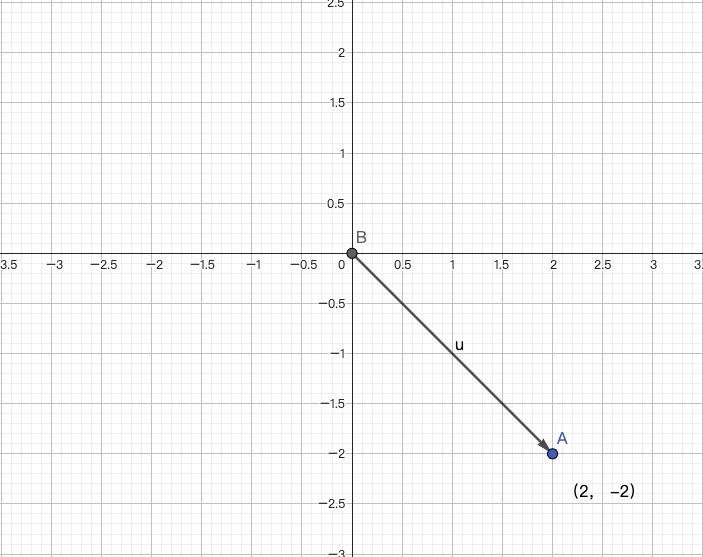
\includegraphics[width=0.5\textwidth]{asset/20230825222021.png}
  \caption{}
  \label{fig:img4_1}
\end{figure}

这个向量在平面直角坐标性里面可以用一个箭头来表示, 然后拿矩阵和向量做一个乘法运算会得到什么结果呢?让我们先来计算一下:

\begin{align*}
  \begin{split}
    & \begin{bmatrix} cos90^\circ & -sin90^\circ \\ sin90^\circ & cos90^\circ \end{bmatrix}
    \begin{bmatrix} 2 \\ -2 \end{bmatrix} 
    = \begin{bmatrix} 2cos90^\circ + 2sin90^\circ \\ 2sin90^\circ - 2cos90^\circ \end{bmatrix} 
    = \begin{bmatrix} 2 \\ 2 \end{bmatrix}
  \end{split}
\end{align*}

再把得到的这个向量也放到坐标系里去(图: \ref{fig:img4_2}):

\begin{figure}[ht]
  \centering
  \caption{}
  \label{fig:img4_2}
  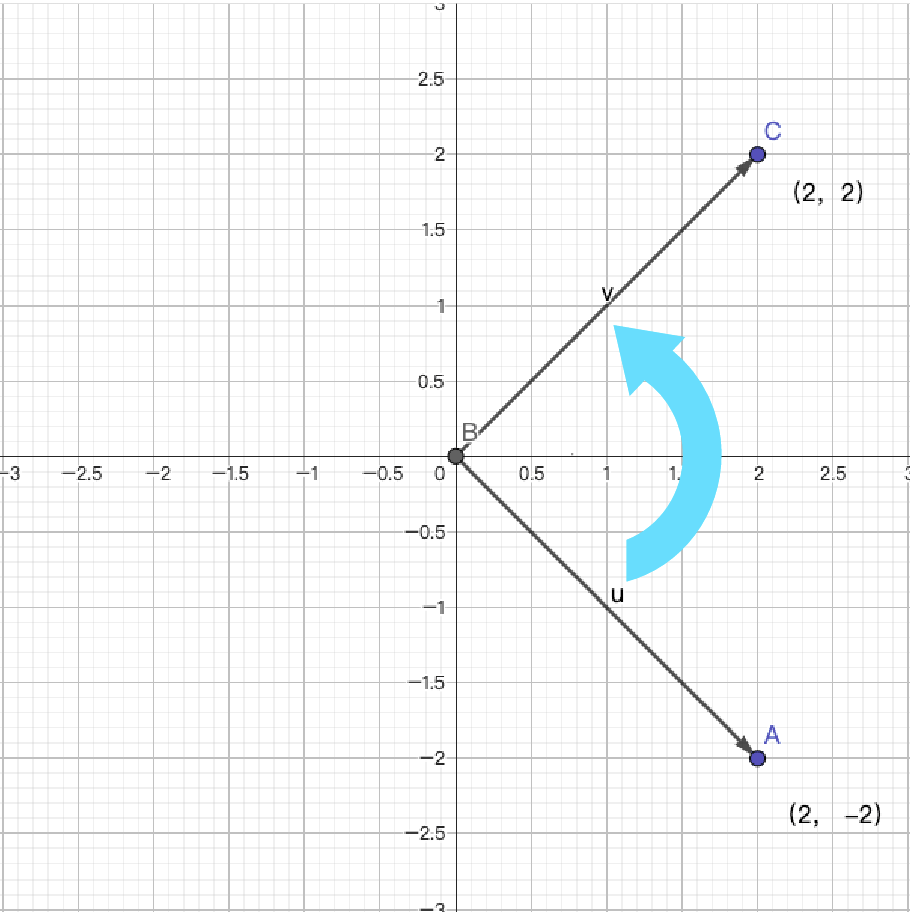
\includegraphics[width=0.5\textwidth]{asset/20230825225602.png}
\end{figure}

我们发现从几何意义上面来说相当于逆时针旋转了 90 度. 所以矩阵在几何上面对应的意义是这个例子里面的旋转变换. 把一个向量旋转一下, 然后这个 90 度就是这个矩称里面的三角函数值的度数. 

除了旋转之外, 还有一个是可以拉伸, 拉伸在之后的课程里面会碰到, 这里给大家举一个旋转的例子, 带大家感受一下矩阵的几何意义. 

\section{矩阵的转置}

矩阵的转置就是沿对角线为对称轴, 把矩阵翻转一下. 或者说这个矩阵行列进行互换. 我们在 Python 课程中后面两节有讲到数据的行转列, 忘记的小伙伴可以再回去复习一下. 

也就是说,本来$1 \quad 2 \quad 3 \quad 4$是第一行, 转置了之后就变成了第一列. $5 \quad 6 \quad 7 \quad 8$是第二行转置了之后第二列, 后面的第三行变成第三列, 这个叫做转置:

\begin{align*}
  \begin{bmatrix} 1 & 2 & 3 & 4 \\ 5 & 6 & 7 & 8 \\ 9 & a & b & c \end{bmatrix}^T
  \Rightarrow \begin{bmatrix} 1 & 5 & 9 \\ 2 & 6 & a \\ 3 & 7 & b \\ 4 & 8 & c \end{bmatrix}
\end{align*}

这个部分还是很好理解. 

\section{矩阵的逆}

矩阵的逆有点像数里面的除法, 就是矩阵乘上它相对应的逆之后, 得到了一个单位矩阵, 这个单位矩阵它是只有在斜对角上是 1, 其他地方的元素全部都是 0 的一个状态. 

\begin{align*}
  \begin{split}
    A^{-1}\mbox{满足}:AA^{-1}=I, \mbox{其中 I 为}
    \begin{bmatrix} 1 & \cdots & 0 \\ \vdots & \ddots &\vdots \\ 0 & \cdots & 1 \end{bmatrix}
  \end{split}
\end{align*}

求解方程组, 就是通过求矩阵系数的逆去做的. 当然逆的作用在高等代数里面非常多, 就不一一缀述了. 大家先知道是怎么一回事, 后面还会专门去讲. 

这里再给大家说一个题外话, AI 这个行业虽然现在世界上中国和美国是并驾齐驱的两个大国. 就是在 AI 领域基本上前沿的研究主要都是中美两国的研究人员做出的. 但是在这个领域里面的文献资料什么的还是以英文为主, 所以我也建议大家多关注一下或者多提升一下自己的英语能力. 你不能拿到一篇 AI 的论文, 想了解它这里面的算法原理以及它是怎么实现的, 可还看不懂 \footnote{之后我会专门写一篇如何去读论文的文章,放在「BI」部分写吧,大家可以关注我后续课程。}. 

而且我有自己的一些感受可以跟大家分享一下, 越是这种专业性比较强的领域, 其实英语上手的难度就越不大. 首先不可能像 GRE 阅读题那样考到怀疑人生, 看完 GRE 阅读再回头看托福的阅读题, 就像是大学教材和初中教材一样那种感觉. 所以某一个领域的东西它的语法结构不会很复杂. 只需要掌握那个领域特殊的一些术语就行了. 剩下的语法规则我觉得高中英语就够了. 

这个不应该成为大家一个障碍, 所以推荐大家从现在开始就去提升一下自己的英文方面的阅读能力. 从阅读开始再慢慢的扩展到其他领域. 
% \chapter{数学导论 - 概率统计基础:随机变量}
\begin{figure}[ht]
  \centering
  
\includegraphics[width=1\textwidth]{asset/96cee23e-7016-44d9-909d-28b64c0b98e7.png}
\end{figure}
\newpage

本节课, 开始学习概率\&统计. 

我的课程的内容其实是比较核心的内容了, 也就是不需要大家特地去拾起什么高等代数这些书. 那些不需要, 也比较耽误时间. 

\section{概率\&统计}

正式开始之前, 先来看一下这几个描述:

\begin{enumerate}
  \item 平时不好好学习,考试的时候\textcolor{blue}{不确定}能否及格
  \item 太阳\textcolor{blue}{一定}是从东方升起的
  \item 绝对\textcolor{blue}{不可能}先经历明天, 再经历昨天
  \item 赌徒\textcolor{blue}{有可能}在赌场用100美元赢到1,000万美元
\end{enumerate}

这四句话里面都有一些「表示程度」的词语, 我不知道大家有没有注意到, 比如说「不确定」、「一定」、「不可能」、「有可能」, 这些就代表了在概率里面要讨论的三种事件. 

首先说到不可能, 对应着\textbf{不可能事件}; 而一定怎么样怎么样, 就对应\textbf{必然事件}; 

不可能事件就是一定不可能发生的; 必然事件是一定发生; 

剩下的不确定或者说有可能, 对应的\textbf{随机事件}, 就是它既有可能发生, 也有可能不发生. 这一部分, 就是概率学里面关注的一个重点. 因为前两种情况都都太简单了, 没研究的必要. 

概率有一个取值范围, 取值范围为0到1之间. 可以把它理解成一个百分比, 1就是100\%. 不可能比100\%还多了, 不会像361度那样, 多一度的热爱. 科学不讲这个东西, 100\%就是满了, 0就是0\%. 所以概率取值范围是在0-1之间. 

100\%发生的事件不就是一定发生的吗? 所以$P=1$对应必然事件. 0\%的可能性发生的事件就是一点可能都没有, 所以它是不可能实现. 介于两者之间就是随机的, 就是概率发生的大小. 30\%、50\%、70\%都是不确定的. 

\begin{itemize}
  \item 概率的取值范围: $0 \leq P \leq 1 $
  \item $P = 0$: 不可能事件 
  \item $P = 1$: 必然事件 
  \item \textcolor{red}{$0 < P < 1$: 随机事件 <== 概率学关注的重点}
\end{itemize}

来看一个抛硬币的例子: 抛硬币会有两种结果, 要么正面要么反面. 

\begin{figure}[ht]
  \centering
  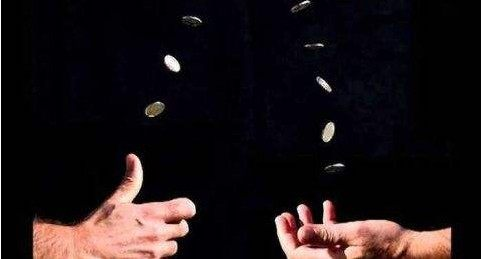
\includegraphics[width=0.7\textwidth]{asset/28420cc4-afeb-4064-97ec-359a2ff38dee.png}
  \caption{抛硬币}
  \label{fig:img5_1}
\end{figure}

当然我相信这个时候肯定有些同学心里面会潜意识的来一句抬杠: “它有可能抛之后还立起来呢”. 确实, 之前也看到过一篇报道就是说有一个大学教授带着他几个学生做抛硬币的实验, 还真抛出来一次立起来. 然后他们通过一系列“严谨的计算”\footnote{这个严谨打个双引号, 因为别的人也看不懂}, 立起来发生的概率是几亿分之一, 所以这个就不好说了. 

概率学上面说的抛硬币是一种抽象化的模型, 就是不扯那些其他乱七八糟东西, 什么立起来, 就把它想象成一个理想化的模型, 要么正面要么反面. 它们出现正面或者反面的概率是相等的, 都是1/2. 

每一次抛硬币就是一次随机事件, 这个事件有可能是正面朝上, 也有可能是反面朝上, 事先不能够确定. 然后根据抛硬币的模型可以提出三个问题:

\begin{itemize}
  \item 第一个问题: 单次抛掷, 正面朝上反面朝上的概率都是1/2, 那么第一次和第二次都出现正面朝上的概率应该怎么样计算? 
  \item 第二个问题: 甲是一个普通人, 他抛硬币正面朝上概率如前所述就是正面朝上0.5, 反面朝上也0.5. 乙是一个赌神, 他有一些办法,可以使正面朝上的概率是0.7. 那怎么描述让乙来抛硬币时正面朝上的概率? 直接说P等于0.7吗? 但是在普通人抛硬币的情况下, 这个P正面朝上是等于0.5. 同一个东西就出现不同的结果了. 
  \item 第三个问题: 第一次第二次抛掷均是正面朝上, 那第三次抛掷还出现正面朝上的概率还是1/2吗? 会不会和前两次有关呢? 
\end{itemize}

\section{联合概率}

先来看一下第一个问题, 第一个问题是说, 单次抛掷正面朝上反面朝上都是1/2. 那两次都正面朝上概率怎么样计算? 

首先, 这个事件是由两个先后的步骤组成: 第一次和第二次. 然后这个事件的概率是有两个步骤各自的概率相乘得到的. 第一次正面朝上在这里用 $P_{\mbox{正正}}$ 来表示, 两次都是正, 等于$\frac{1}{2} \times \frac{1}{2}$, 所以两次都出现正面的概率是1/4: 

\begin{align*}
  P_{\mbox{正正}} = \frac{1}{2} \times \frac{1}{2} = \frac{1}{4}
\end{align*}

有的同学, 尤其是刚开始接触概率同学会问: 你凭什么说事件的概率要由组成它的步骤的概率相乘得到呢? 凭啥不能相加呢? 那为啥不能是1/2加1/2, 或者说是其他运算呢? 来看图 \ref{fig:img5_2}:

\begin{figure}[ht]
  \centering
  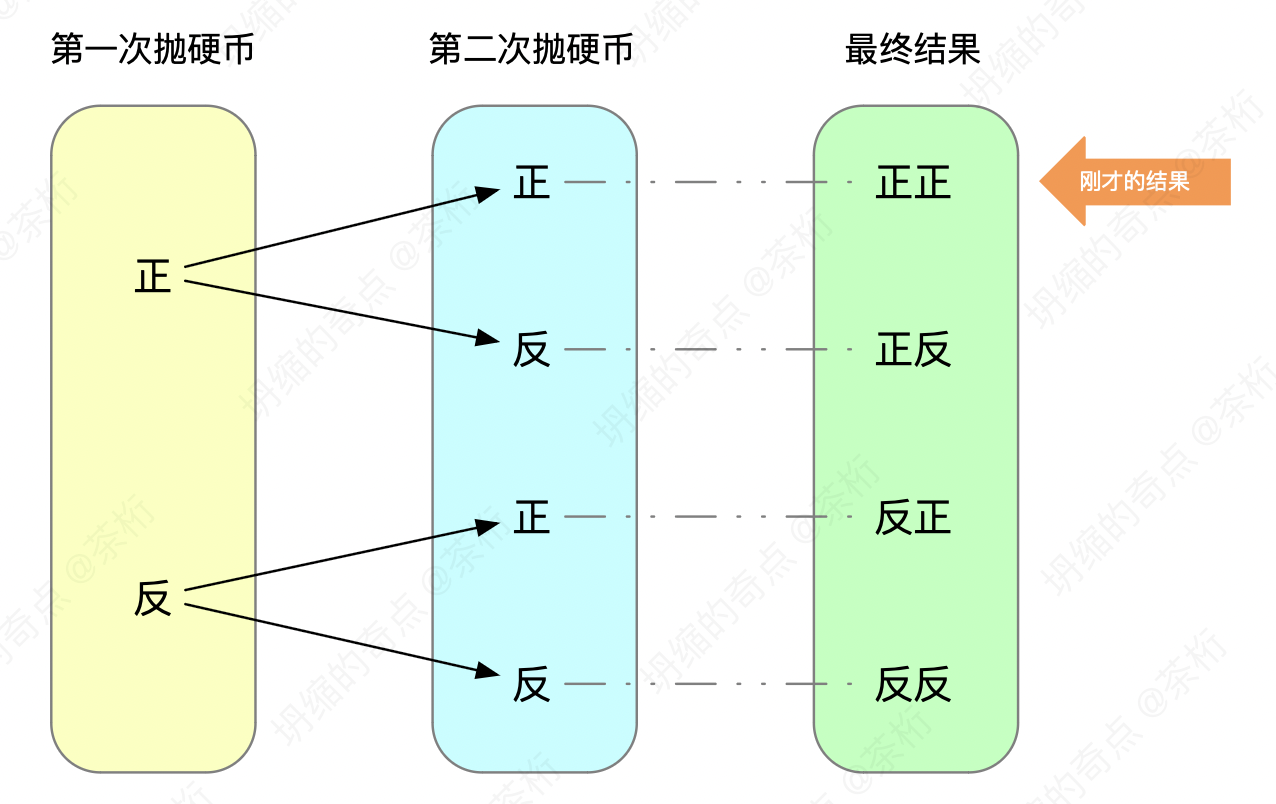
\includegraphics[width=0.7\textwidth]{asset/bd947955-687e-49b7-a430-c6921cd49504.png}
  \caption{抛硬币步骤}
  \label{fig:img5_2}
\end{figure}

首先来看一下, 第一次抛掷会出现两种结果, 要么正要么反. 第二次抛掷它是不是也有两种情况, 要么正要么反. 而第一次和第二次出现结果的组合总共有多少种? 是不是$2 \times 2 = 4$种? 就像这里的\textit{正正、正反、反正、反反}一共4种. 然后两次抛掷均为正面的情况, 只占一种, 所以它最终概率就是1/4. 总共有四种情况, 两次均为正只占一种情况, 所以不就是1/4吗? 

通过这个简单的例子得出一个什么样的结论呢? 就是这个事件如果由多个步骤完成的话最终可能出现的结果种类就是你每一步能出现的那个结果的数量相乘得到的. 

比如说第一步只可能出现正反两种结果, 第二步也是只可能出现要么正要么反两种结果, 那就是$2\times 2$总共等于4种结果. 如果再来第三次抛掷那又是多少, 就又是正或者反. 那就是$2\times 2\times 2=8$. 所以就引出了「联合概率」的这个概念. 

把A事件(就是第一次抛至正面朝上)发生的概率用$P(A)$表示. 

B事件(指第二次抛至正面朝上发生的概率)用$P(B)$来表示. 

A和B同时发生的概率用$P(AB)$或者$P(A,B)$来表示. 这两种都行, 都是等价的, 表示他们俩同时发生. 

如果A和B是相互独立的. 什么叫相互独立? 就是A发生不发生, 跟B一点关系都没有. 同样的B发生不发生, 跟A也没啥关系, 对A也没有任何影响, 你爱咋咋. 就像两口子吵架的一样, 你想干啥干啥, 你想剁手就剁手, 你想买东西买东西. 就是一个相互独立事件, 谁也不理谁谁也不需要管谁. 在这种情况下, 它们的联合概率就是它俩同时发生的概率, 也就是他们各自发生的概率乘在一起. 也就是说: \textbf{如果A和B它是相互独立的,则$P(AB) = P(A)P(B)$}

如果A和B它不是相互独立的, 那这个$P(AB)$它要怎么去计算呢? 这里就需要去通过一些概率的定义方面去做. 

\section{条件概率}

再来看一下第二个问题: 普通人和赌神抛硬币出现正面朝上概率是不一样的. 普通人正面朝上概率是0.5, 赌神正面朝上概率是0.7. 这两种概率表示同一种结果, 都是抛硬币正面朝上, 但是他们这个概率值是不一样的. 

\begin{itemize}
  \item 普通人 => P(正面朝上) = 0.5 
  \item 赌神 => P(正面朝上) = 0.7
\end{itemize}

单纯看这个P(正面朝上)我也判断不出来它这个概率究竟应该是0.5还是0.7. 所以在这里应该怎么样去处理呢? 虽然他俩都表示同样一种结果, 但是先决条件不一样, 一个是让普通人来抛, 另一个是让赌神来抛. 两个先决条件不一样, 最终结果肯定是不一样的. 所以在这里就引入了「\textbf{条件概率}」. 

\textbf{条件概率表示在某个先决条件已发生的情况下, 某一个事件发生的概率}. 先决条件与讨论的事件是有关联的, 就不像刚才那个例子里面说的一样, 第一次抛掷和第二次抛掷它是相互独立的, 谁也不用管谁, 在这里条件概率是有关联的. 

key $\Rightarrow$ 事件的先决条件不同

A在这里作为先决条件, 这个例子里面的先决条件就是操作者是赌神还是普通人. B是要讨论的研究的这个事件. 所以当A确定的情况下, B发生的概率用这个 $P(B|A)$ 来表示. 杠后面的条件已经发生的条件下, 杠前面的事件发生的概率有多少. 

在这里理解起来就是选定了普通人来抛硬币, 正面朝上的概率就是0.5, 正面朝上后面要加上一个杠, 然后在杠后面添加上普通人三个字:$P(B|\mbox{普通人})$

赌神也是一样, 在正面朝上后面添加上一个杠, 杠后面再加上赌神两个字: $P(B|\mbox{赌神})$.  表示操作者不同, 发生同一事件的概率是不一样的, 这个叫做条件概率. 

那联合概率和条件概率有什么联系吗? 

他们确实是有一些联系, 先来回顾一下联合概率: A和B是相互独立的, 那就等于它们各自发生的概率直接相乘得到的: $P(AB) = P(A)P(B)$

那如果A和B不是相互独立的怎么去计算它? 怎么计算A和B都发生的联合概率? 在这里就可以结合条件概率去做. 先求得A发生的概率是多少, 然后再来看A已经确定发生的情况下我B发生的概率是多少. 现在回过头来看刚才那个情景:\textbf{从赌神和普通人中随机选择一个人抛硬币}. 

$P(A)$代表从赌神和普通人两个人当中选出赌神的概率等于0.5对吧? 然后赌神抛出正面朝上的概率是0.7.  也就是在已经确定 A=赌神 的情况下, $P(B|A)$就相当于$P(B|\mbox{赌神})$, 抛出正面朝上的概率就等于0.7. 现在再来看$P(AB)$, 就等于$P(B|A)P(A)$, 所以就等于$0.5 \times 0.7=0.35$. 

总结一下联合概率:
\begin{itemize}
  \item 若A和B是相互独立的, 则 $P(AB) = P(A)P(B)$ 
  \item 若A和B不是相互独立的, 如何计算 $P(AB)$? 
  \item $key: P(AB) = P(B|A)P(A)$
\end{itemize}

这个部分其实还是已经很偏基础了, 正常逻辑思维能力都可以跟得上. 如果一时没跟上的也没有关系, 可能注意力不集中,再多看几遍就可以了, 自己再查查资料. 记住, \textbf{任何时候除了在课堂上学过的东西之外还需要拥有自学的能力}. 不管是在大学读本科、读研还是读博, 甚至说已经工作了, 或者说是在大学当老师怎么样, 如果没有自学的能力我觉得是很可怕的一件事情. 因为不可能所有的事情都能恰好找到适合你的那个老师或者机构帮你解决这个问题, 学习这个事还是要靠自己. 

再来看一下第三个问题: 第三个问题是前两次都是正面朝上, 那第三次抛掷还出现正面朝上的概率仍然是1/2吗? 答案是: 仍然是. 因为第几次, 就算是第n次也好, 它相互之间都无关. 第三次和第七次之间、和第六次、第五次、第十八次之间都是没有任何关联的, 都是独立的, 不相关. 所以第三次抛掷概率还是1/2. 

但是这一点有些人会觉得有点不大能理解为什么. 比如说, 在现实生活当中, 如果我连续抛四次硬币, 前三次都已经是正面了, 那第四次还是正面的概率就会觉得好像有点小. 但其实第四次出现正面朝上的概率仍然是1/2. 但是为什么会有这样的感觉, 就感觉好像第四次不大可能是正面了? 是因为心里面所想象出来这个概率小是针对什么事情来说, 概率小是\textbf{四次都出现正面朝上}这件事情概率小, 而不是\textbf{第四次抛出正面朝上}概率小, 这两个是不一样的. 

判断这两个事件是否独立的一个判断标准其实就是要看$P(B|A)$和$P(B)$它是否是相等. 如果他们俩是相等的就代表B发生的概率等于在A已经确定发生的情况下B发生的概率. 什么意思呢? 就是不管你A发生不发生, B的概率就是这么多, 那就是说A和B没有关系. A发生B的概率是这么多, A不发生B概率也是这么多, 这就是判断两个事件是否独立的一个标准. 

\section{随机事件}

接下来再来正式的说一下随机事件, 它表示在随机试验中可能出现也可能不出现, 而在大量重复试验中具有某种规律性的事件, 简称事件. 就比如下面这些例子:

\begin{itemize}
  \item 抛硬币, 正面朝上是一个随机事件
  \item 反面朝上亦是一个随机事件
  \item 掷骰子朝上的点数为偶数是一个随机事件. 
\end{itemize}

随机变量是什么概念? 刚才说随机事件, 因为想用数学化的语言去解决它, 去对它做一些处理. 所以希望能把这个随机事件的结果给它数量化表示, 数量化表示出来的这个结果就叫做随机变量. 

\begin{itemize}
  \item 一次随机试验可能出现的结果的数量化表示
  \item 一般用大写字母表示,  如X, Y
\end{itemize}

比如说我抛掷两个骰子得到的向上点数之和就是一个随机变量. 描述点数有可能用一个二元数组, 比如说第一个骰子4, 第二个骰子是2, 那在这种情况下可能就是用一对数来表示. 但是在这里, 通过点数之和可以把它转换成可操作的一个数量. 

\begin{itemize}
  \item 抛掷两个骰子得到的向上的点数之和就是一个随机变量
\end{itemize}

随机变量也分两种:「连续型」和「离散型」. 
\begin{itemize}
  \item 连续型随机变量, 如街头采坊一个人, 他/她的身高
  \item 离散型随机变量, 如街头采坊一个人, 他/她的性别
\end{itemize}

连续型就是随机变量的取值可以是连续的, 比如我街上在采访一个人, 他这个身高是178.65公分, 或者说他是164公分, 或者是183公分. 这个数值之间还有其他数值可以连续, 数字之间没有这种间隔, 不是跳跃性的. 更确切的说法解释就是: 178公分 - 180公分, 这两个确切数值之间还有其他的连续数值. 

离散型的随机变量就是有跳跃性的, 只能取规定的那些, 值与值之间是没有其他的值可以连续. 比如说在班上抽查学生, 抽出来是男生还是女生, 性别没办法用数字去表示, 所以就做一个转换, 比如说男生是-1女生是1, 那这样子就可以用随机变量的概念去处理这个概率事件. 男生对应着-1, 女生对应着+1, -1和+1之间没有其他值. 

做一些机器学习方面分类的时候其实也是一样的, 离散型的随机变量就是取值和取值之间没有相邻的量, 经常会把一些标记这种类别的东西给它转换为数字. 比如鉴别花的种类, 花可能有十几种, 如果按照中文名去做分类的话那计算机没办法对这种名字去做处理, 而在机器学习当中如果要鉴别花的种类, 把它转换成数字的形式去处理. 比如:月季对应着1, 玫瑰对应2, 百合对应5等等. 给它标一个数字, 实际上在机器学习的工程当中, 都是用独特编码还有其他的一些编码去做, 不是单纯的给它附一些值. 

\section{数学期望}

随机试验的结果可以有怎样定量的期待, 这个就表示了这个数学期望的一个含义. 什么意思呢? 就是有的时候, 在我做随机实验之前就能有一个大概的了解, 有一个预估. 如果做了这个实验我的回报, 或者说我的损失, 或者说这个实验结果会是怎么样的. 

比如一个人打算去赌博, 手里趁两钱去澳门了. 他有两种可能的结果, 一个是他赌赢了, 给他1,000美金, 概率只有0.001; 另一个就是他的赌资50美金打了水漂, 概率是0.999. 基本上就是赌赢的概率非常小. 赢都是小概率事件, 所以对于这两种结果他是可以提前预判到的. 那如何根据这些已经得到的信息来做一个对结果的预估呢? 这个就是数学期望. 就是能够获得的这个平均回报是多少, 就是说每种可能的结果(图: \ref{fig:img5_3}). 

\begin{figure}[ht]
  \centering
  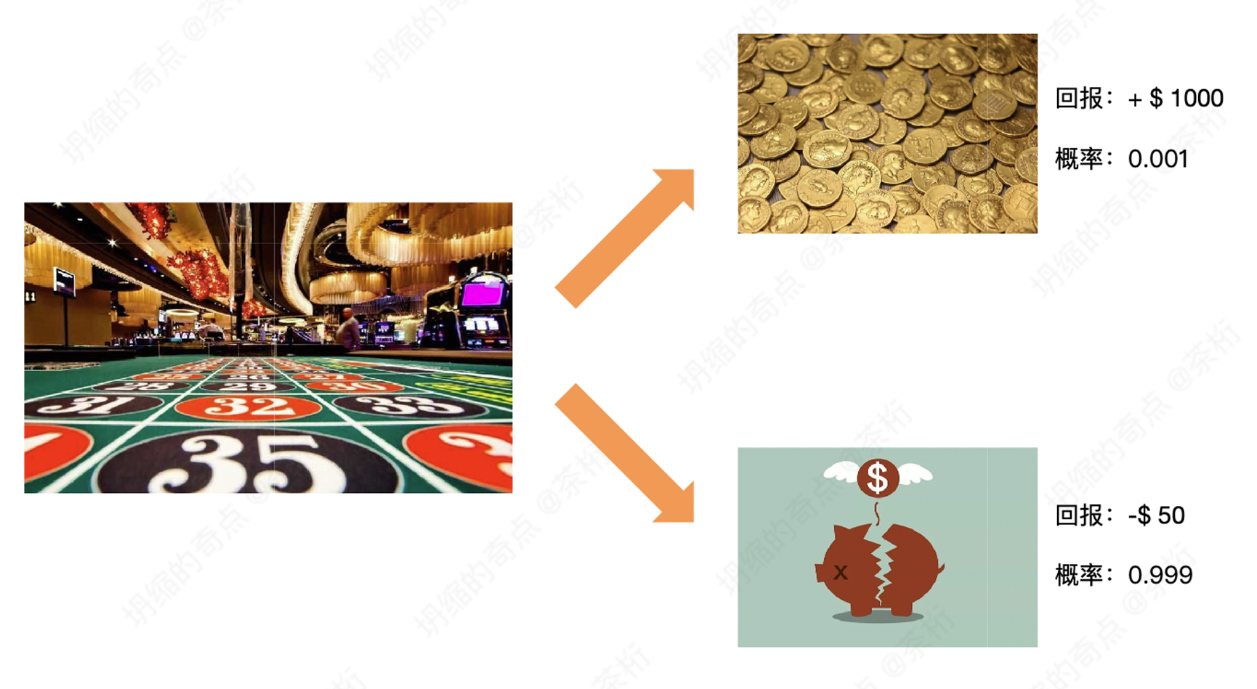
\includegraphics[width=1\textwidth]{asset/86da64b2-45f2-42c2-add4-d7db67f5cf82.png}
  \caption{}
  \label{fig:img5_3}
\end{figure}

在经过大量试验之后, 能够收到的平均回报是多少呢? 就是回报金额乘以概率, 最后两个计算结果相加:

\begin{align*}
  E(X) = 1000 \times 0.001 + (-50) \times 0.999 = -48.95
\end{align*}

这个$E(X)$就代表了数学期望, $E$ 代表了$\mathord{Expectation}$, 代表了期望. 这里的规则就是每种可能的结果乘上结果对应的概率, 再把所有的乘积加在一起, 其实也很简单对吧. 我相信大部分人听到这里都已经听懂了. 

那再来看下一个例子, 这个例子也很有趣: 有甲乙两个人进行赌博, 对于每一局而言,两个人获胜的几率都是相等的, 就是五五开, 谁也不占谁便宜. 比赛是五局三胜制, 最终的赢家可以获得100美元的奖励. 在第四局比赛开始前, 由于特殊情况需要终止比赛, 而在前三局甲已经赢了两局, 乙赢了一局. 那问题来了, 在没办法继续比赛的情况下, 应该如何公平的分配这100美元呢? 

就是说, 不把这后面两局给比出来的话不知道最终的结果, 因为前三局并不是甲都赢了或者乙都赢了, 甲只赢了两局乙只赢了一局, 谁都没有构成3胜. 所以这个时候就需要用到数学期望的知识去去判断一下, 甲如果这个比赛继续进行下去最终获胜的概率是多大, 然后通过他的这个获胜概率来预估一下他应该对应的奖金. 同样的对乙也做这样的判断, 如果比赛进行下去, 乙最终获胜的概率有多大. 然后根据获胜的概率来看一下乙他应该获得奖金的期望值是多少, 就是预估值是多少.

解: 若比赛继续, 甲只需要再赢一局即可获胜, 乙需要两场全赢. 

\begin{itemize}
  \item \textbf{甲}最终\textbf{不获胜}的概率: $P(\mbox{甲负}) = \frac{1}{2} \times \frac{1}{2} = \frac{1}{4} $
  \item \textbf{甲}最终\textbf{获胜}的概率: $P(\mbox{甲胜}) = 1 - P(\mbox{甲负}) = \frac{3}{4}$ 
  \item \textbf{乙}最终\textbf{获胜}的概率: $P(\mbox{乙胜})  = \frac{1}{2} \times \frac{1}{2} = \frac{1}{4}$ 
  \item \textbf{乙}最终\textbf{不获胜}的概率: $P(\mbox{乙负}) = 1 - P(\mbox{乙胜})  = \frac{3}{4}$ 
  \item 甲可获得的奖金期望值: $E(\mbox{甲}) = 100 \times \frac{3}{4} + 0 \times \frac{1}{4} = 75$ 
  \item 乙可获得的奖金期望值: $E(\mbox{乙}) = 100 \times \frac{1}{4} + 0 \times \frac{3}{4} = 25$
\end{itemize}

来一步一步看, 这个比赛如果比赛继续的话甲只需要再赢一局就可以了, 乙需要两场都赢. 所以最终甲他不获胜的概率, 假如说点背最后两局都输了, 那输的概率是$\frac{1}{2} \times \frac{1}{2}$, 乘在一起呢是1/4. 这就是甲最终不获胜的概率. 

然后就知道了, 甲最终要么获胜要么不获胜, 只有这两种结果, 不可能出现第三种情况. 就拿1去减这种情况, 就对应的这个甲最终获胜的概率. 甲获胜的所有情况加在一起概率之和为1, 通过1去减1/4就得到3/4. 

同样的道理, 乙也是一样, 乙必须两场全赢, 所以乘在一起等于1/4. 乙最终不获胜也拿1去减, 等于3/4. 

再来分别看一下, 按照数学期望的定义, 甲如果继续比赛下去有哪两种结果? 赢或者不赢. 赢对应的奖金有100, 概率呢是3/4, 输的奖金就是零, 一分钱没有, 甲输的概率是1/4, 所以甲获得奖金的期望值是75. 

乙去做同样的运算, 获胜的概率是1/4, 获胜了也是能拿100块钱, 再加上不获胜就一分钱没有, 不获胜概率3/4. 这么一乘一加, 乙获得奖金的期望值就是25. 

所以按照75和25的分配方式把奖金给甲和乙分了就行了, 而且保证公平公正, 因为是根据两人各自的胜率、期望值来得到的, 所以是公平的. 

期望还有一些性质:

\begin{enumerate}
  \item $E(C) = C$, $C$ 为常数 
  \item $E(CX) = CE(X)$, $C$ 为常数 
  \item $E(X+Y) = E(X) + E(Y)$ 
  \item $E(XY) = E(X)E(Y)$,  当$X,Y$相互独立时
\end{enumerate}

第一个, 如果是对一个常数去求期望的话, 就是参数本身. 就像常函数一样, $f(x) = 3$, 始终都是3. 

第二个性质, $E$乘上$CX$, 就是它的随机变量乘上一个常数, 等于把这个常数拿出来和这个随机变量的期望值相乘. 

如果是两个随机变量相加, 是把他们各自的期望值加在一起, 等于他们俩相加的期望值. 

如果两个随机变量相乘只有当X和Y相互独立的时候这个式子才成立. $E(XY)$等于$E(X)$乘上$E(Y)$. 如果X、Y不是相互独立的话, 就只能根据这个期望值的定义去做. 期望值的定义就是每种结果乘上这个结果对应的概率值, 再把所有的乘积加在一起. 

\section{方差}

思考一个例子: 投掷一枚骰子, 它向上的点数期望值是多少呢? 来计算一下:

\begin{align*}
  E(\mbox{点数}) & = \frac{1}{6} \times 1 + \frac{1}{6} \times 2 + \frac{1}{6} \times 3 + \frac{1}{6} \times 4 + \frac{1}{6} \times 5 + \frac{1}{6} \times 6 \\
  & = 3.5
\end{align*}

根据这个计算,$1 \quad 2 \quad 3 \quad 4 \quad 5 \quad 6$ 出现机会均等, 都是1/6, 算出来结果期望值点数3.5. 但是朝上点数不可能总是3或者4, 各个点数出现的次数都是均等的. 所以单纯的靠期望值这么一个量去表示一个随机事件可能会有其他一些方面信息的缺失. 也就是说这句话里面出现的矛盾, 期望值3.5似乎是在3和4之间出现的情况最多, 但是实则是各个点数都一样, 怎么刻画呢? 

这里就用到了方差的概念. 方差是度量随机变量和它的数学期望之间偏离程度的一个量. 定义式: 

\begin{align*}
  D = \sigma ^2 = \sum^N_{i=1} \frac{(X-E(X))^2}{N}
\end{align*}

定义式中, 一般用大写字母D来表示, 也可以用$\sigma^2$来表示. 如果给它开个平方的话, 就叫做标准差. 之后也会说到标准差, 标准差用一个$\sigma$来表示. 

等号后面就是这里面所有种情况($\sum_{i=1}^N$), 每种情况的取值($X$)减去数学期望的值($E(X)$), 再做一个平方, 然后再除以每一个情况可能出现的这个概率(N). 在这里机会均等, 就像投骰子一样, $1 \quad 2 \quad 3 \quad 4 \quad 5 \quad 6$ 点数朝上概率是均等的. 所以除以一个N, 这个就是方差的一个定义. 

那方差可以帮助去做什么呢? 在这里看一个例子:

A和B两个人工智能模型, 它们在一系列同分布的数据集上的分类准确率如表\ref{fig:table5_1}所示, 判断哪个模型表现更好:

\begin{table}[ht]
  \centering
  \begin{tabular}{lllllll}
  \midrule
    A & 90\% & 92\% & 93\% & 91\% & 92\% & 94\%\\
    B & 88\% & 97\% & 90\% & 96\% & 94\% & 87\%\\
  \bottomrule
  \end{tabular}
  \caption{A和B的分类准确率}
  \label{fig:table5_1}
\end{table}

现在有A和B两个人工智能模型, 它们在一系列同分布的数据集上的分类准确率就如上面展示的这样. 现在需要判断哪一个模型表现更好. 

同分布的意思就是它们俩判断的数据集概率模型是一样的, 不可能出现一个是高斯分布, 一个是泊松分布. 这两个本来分布都不一样的模型, 判断精确度就不可能去做一个评判了, 所以肯定是同分布, 或者说就是同样的数据集, 同样的数据集去做这个分类. 

总共判别6次, A的准确率是第一行表示, B的准确率是第二行表示. 

先从均值, 也就是数学期望的角度去判断一下, 看他们有没有优劣之分. 

\begin{align*}
  E(A) = \frac{90\% + 92\% + 93\% + 91\% + 92\% + 94\%}{6} = 92\% \\
  E(B) = \frac{88\% + 97\% + 90\% + 96\% + 94\% + 87\%}{6} = 92\%
\end{align*}

A通过运算得出来结果是92\%, 各次分类的结果平均而言准确率是92\%. 就是说92\%的样本A模型可以正确识别, 剩下8\%判断错误. 

B运算得到的也是92\%. 所以从均值或者说期望的角度去判断是没办法说哪个好哪个不好. 

这时候再来看一下方差, 从方差的角度判断 \textit{(由于公式过长会导致板式出错,所以将原本一行的相加折成了两行)}:

\begin{align*}
  \sigma^2(A) & = \frac{(0.9-0.92)^2 + (0.92-0.92)^2 + (0.93-0.92)^2}{6} \\ & + \frac{(0.91-0.92)^2 + (0.92-0.92)^2 + (0.94-0.92)^2}{6} \\ 
  & = 0.000167 \\
  \sigma^2(B) & = \frac{(0.88-0.92)^2 + (0.97-0.92)^2 + (0.90-0.92)^2}{6} \\ & + \frac{(0.96-0.92)^2 + (0.94-0.92)^2 + (0.88-0.92)^2}{6} \\
  & = 0.00135 \\ 
  \mbox{因为}: & \quad  \sigma^2(A) < \sigma^2(B) \\
  \mbox{所以}: & \quad \mbox{模型A的表现更稳定更好. }
\end{align*}

A的方差计算后数值为$0.000167$, B是$0.00135$ \footnote{这里是我自己手工计算得到结果和程序计算相印证, 应该是没有错误的. }. 

然后就判断出来A的方差比B的方差要小, 小代表什么呢? 回忆一下方差里面的定义, 就是这个随机变量离期望的偏离程度. 那方差越小就代表偏离程度越小, 偏离程度越小代表这个模型表现的比较稳定, 比较稳定就不会起伏很大. 

有些同学可能状态起伏特别大, 这次能考班上第一, 下一次有可能就只能考班上第十几名. 从这个角度来看A模型的表现就比B要更稳定, 所以模型A的表现更好. 这就是方差可以帮我们做的事情. 

有的同学可能要问: 为什么在方差的定义式里面要加上平方这项? 不用平方不行吗? 

Why平方? $\sigma^2 = \sum^N_{i=1}\frac{(X-E(X))^2}{N} \quad ?$.

不用平方不可以吗? $\sigma = \sum^N_{i=1}\frac{X-E(X)}{N} \quad ?$

确实是不行, 比如说图\ref{fig:img5_4} 的例子:

\begin{figure}[ht]
  \centering
  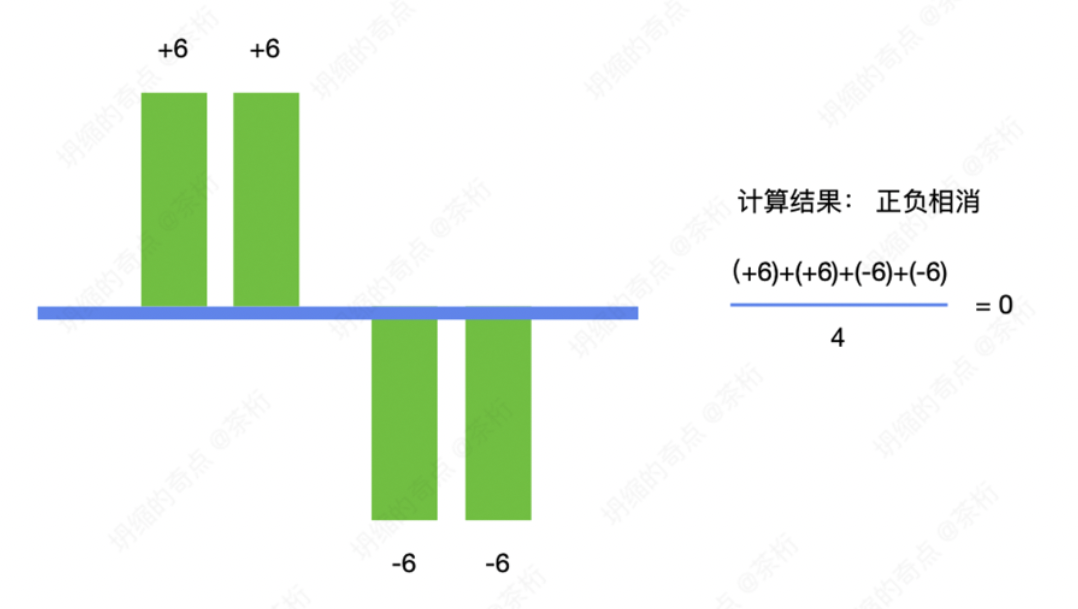
\includegraphics[width=0.9\textwidth]{asset/713e717f-8a86-42db-83e6-b74c5afe50a4.png}
  \caption{}
  \label{fig:img5_4}
\end{figure}

蓝色的横线代表均值, 也就是期望. 绿色的柱子代表了各个量, 相对于数学期望的一个偏差值. 比如结果比数学期望分别为(+6,  +6,  -6,  -6), 如果不把它平方一下, 会发现它就正负相消了, 最终得出的结论方差为零. 那这是显然不可能的事对吧? 所以要在这里加一个平方. 

有的脑子好一点的同学可能还会问: 那绝对值行不行? 绝对值按照道理来说其实是可以的, 没有问题. 但是绝对值运算在数学处理里面不太好去处理, 因为还得判断绝对值符号. 比较什么时候取正、什么时候取负, 这样子去做的话用平方会比较好一点. 

\hypertarget{方差的性质}{}
来看一下方差的一些性质:

\begin{enumerate}
  \item $D(C)=0$,  $C$ 为常数
  \item $D(X+C) = D(X)$, $C$ 为常数
  \item $D(CX) = C^2D(X)$, $C$ 为常数
  \item $D(X+Y) = D(X) + D(Y) + 2Cov(X,Y)$ \hyperlink{协方差}{$Cov$ 意为协方差}
  \item $D(X+Y) = D(X) +D(Y)$,  当X和Y相互独立时
  \item $Cov(X, Y) = E\{[X - E(X)][Y-E(Y)]\}$:  协方差
\end{enumerate}

方差的性质就是这些, 对于常数而言方差是0, 因为很显而易见, 它都没有偏离了, 始终取值就那一个, 就等于0. 

以上的这些式子, 大家看一下就好, 就不再一一缀述了. 

\section{标准差}

接下来就说说标准差, 标准差我刚才提到过, 直接对方差开个平方($\sqrt{D}$). 他有一个好处就是, 度量的效果和方差是一致的. 

\begin{align*}
  \sigma  = \sqrt{\sum^N_{i=1}\frac{(X-E(X))^2}{N}}
\end{align*}

设想一下, 一个量的方差大于另外一个量的方差, 比如说A大于B, 那开平方之后, 标准差还是保持一致的. 大小关系不会变. 但是标准差有一个好处, 方差因为有一个平方, 所以它和随机变量的\textit{量纲}是不一致的. 开一个平方之后, 在量纲方面就能和随机变量保持一致. 

量纲其实就是单位, 千克、米、秒这些叫做量纲, 其实就是单位. 所以标准差:

\begin{itemize}
  \item 度量效果与方差一致
  \item 量纲和随机变量一致
\end{itemize}

\hypertarget{协方差}{}
\section{协方差}

我们在上面\hyperlink{方差的性质}{方差的性质}中,其中引出了这么一个量, 第4个式子 $D(X+Y) = D(X) + D(Y) + 2Cov(X,Y)$: 当两个随机变量加在一起, 考虑他们和的方差的时候, 是等于各自的方差再加上一个 $2Cov(X,Y)$, 这个概念叫做协方差\textit{Covariance} . 

协方差是用于衡量两个变量的总体误差. 说通俗点就是, 当协方差是正的, 就代表这两个随机变量的变化趋势是相同的. 如果随机变量A大于期望值的时候, 随机变量B也应该大于他的期望值. 如果是小于的情况也是一样. 两个大于同时大于, 两个小于也同时小于. 

如果协方差为负, 那这两个变量的变化趋势就相反了. 一个大于期望值, 另外一个小于, 反过来也是成立的. 

协方差为0的时候代表两个变量没有线性相关性. 

这个「线性相关性」很多书本上面把「\textbf{线性}」两个字给去掉了, 只提「相关性」. 其实是不对的, 如果把\textbf{线性}给去掉, 只说两个变量无相关性, 无相关性就对应着两个变量独立, 但是两个变量除了线性的相关性之外, 还可以有其他非线性的. 

那什么叫线性呢? 也就是说$Y=K(X+B)$这种形式,当X变换的时候,Y也是按照这个放大倍数变换的. 

再换一个严格意义上的例子: $Y=KX$ 这个例子, X扩大K倍Y也是K倍的扩大多少, 这种叫做线性. 

而非线性呢, 比如说$Y=X^2$, X增加了多少, Y增加的量不是乘上一个常数来决定的, 这种叫做非线性. 

所以协方差为0只能说两个变量没有线性相关性, 不能得出两个变量是独立的. 

总结一下协方差:

\begin{itemize}
  \item 用于衡量两个变量的总体误差
  \item 协方差为正: 两个变量的变化趋势相同, 当一个大于其期望值时, 另一个也大于, 小于的情况亦然.
  \item 协方差为负: 两个变量的变化趋势相反, 当一个大于其期望值时, 另一个就小于, 反之亦然.
  \item 协方差为0: 两个变量无线性相关性.
  \item 两个变量独立, 则协方差一定为0, 反之并不一定成立.
\end{itemize}

所以, 协方差为0不一定得出来变量是独立的. 这个可能稍微有点绕, 但是大家只要能把\textit{线性相关性}、\textit{非线性相关性}和\textit{独立}给区别出来就行. 来看一下相关公式:

\begin{align*}
  Cov(X,Y) & = E\{[X-E(X)][Y-E(Y)]\} \\
  & = E\{XY - XE(Y) - YE(X) + E(X)E(Y)\} \\
  & = E(XY) - E[XE(Y)] - E[YE(X)] + E(X)E(Y) \\
  & = E(XY) - E(X)E(Y) - E(X)E(Y) + E(X)E(Y) \\
  & = E(XY) - E(X)E(Y)
\end{align*}

经过一系列运算得到两个随机变量的协方差, 可以表示成两个乘积的期望值减去期望值的乘积. 所以如果$X,Y$是独立的, 那E(XY)等于什么?

当$X, Y$独立时, $E(XY) - E(X)E(Y) = 0 \Rightarrow Cov(X,Y) = 0 $.

接下来这个内容其实就是体现了或者说验证了刚才说的. 就是两个随机变量的协方差如果是正的就代表增长的方向是相同的. 如果是负的就代表了一个增就一个减、一个减就一个增. 

例:表\ref{fig:table5_2} 给出一位同学的历次数学和物理考试的乘积, 试利用协方差判断他的两个科目成绩之间有怎样的关系. 

\begin{table}[ht]
  \centering
  \begin{tabular}{lllllll}
    \midrule
      数学 & 90 & 92 & 85 & 97 & 96 & 98 \\
      物理 & 85 & 95 & 88 & 95 & 93 & 90 \\
    \bottomrule
  \end{tabular}
  \caption{成绩单}
  \label{fig:table5_2}
\end{table}

\begin{align*}
  \mbox{解: \qquad E(数)} & = \frac{90+92+85+97+96+98}{6} = 93 \\ \\
  \mbox{E(物)} & = \frac{85+95+88+95+93+90}{6} = 91 \\ \\
  \mbox{E(数、物)} & = \frac{90 \times 85+92 \times 95 + 85 \times 88 + 97 \times 95 + 96 \times 93 + 98 \times 90}{6} \\ 
  & = 8472.17 \\ \\
  \mbox{两个变量的协方差:} \\  
  Cov(\mbox{数,物理}) & = E(\mbox{数,物}) - E(\mbox{数})E(\mbox{物理}) \\ 
  & = 8472.17 - 93 \times 91 = 9.17
\end{align*}

计算下来,运算得到结果是9.17, 它是大于零的, 所以代表这两个学科的成绩是成一个正相关的关系. 

再来思考一个问题: 大于0的时候, 协方差越大, 关联性越大嘛? 

对于同样的随机变量而言是这样没错. 就比如这一位同学的数学和物理考试成绩, 他又考了几次, 又有了新的数据, 计算出来结果可能比这个9.17大或者小, 那这个时候就可以拿9.17和新的计算出来的协方差的数值去进行一个比较, 越大这个相关性就越大. 

但是如果是不同的随机变量之间就没办法说了. 所以这里有一个概念叫做「相关系数」. 就是协方差除以随机变量的方差, 就把它做一个归一化的处理, 消除了数值本身带来的影响, 那这个就是「简单相关系数」. 还有其它一些不同的相关系数, 比如复相关系数、典型相关系数等等. 关于「相关系数」, 强烈建议大家下来再自己查询一下. 
% \chapter{数学导论 - 图论:图的概念}

\begin{figure}[ht]
  \centering
  \includegraphics[width=1\textwidth]{asset/茶桁的 AI 秘籍_Math_5.png}
\end{figure}

\newpage

今天这节课内容非常少, 少到你可能会认为我偷懒了. 

还真不是, 因为就目前基础来说, 图论这一节没有太多可讲的东西, 重点是带大家混个脸熟. 那么多高强度内容之后, 就当给自己放个假吧. 

\section{图论}

前面说过, 这部分内容相对来说是最轻松的一部分内容. 在图论这里, 我只想带大家简单了解一下图是什么样的一个概念, 以及图有什么样的一些性质. 

其实, 图论要是说开了的话那今天咱们这节课还止不住要写多少内容呢, 所以我就挑了一些最基本的概念. 

首先, 什么是图?

\begin{figure}[ht]
  \centering
  \begin{minipage}[h]{0.4\textwidth}
    
\includegraphics[width=\textwidth]{asset/03be564f-4ce8-45d1-acde-f8e0300c4e6f.png}
    \caption{一张普通的照片}
    \label{fig:img6_1}
  \end{minipage}%
  \hspace{3em}
  \begin{minipage}[h]{0.4\textwidth}
    图论里面的图, 和我们生活当中的图是一样的吗?是指我们图片、或者说我们拍照的相片、亦或是我们的地图吗?
  \end{minipage}
\end{figure}

不是的, 我给大家看一下: 

\begin{figure}[ht]
  \centering
  \begin{minipage}[h]{0.45\textwidth}
    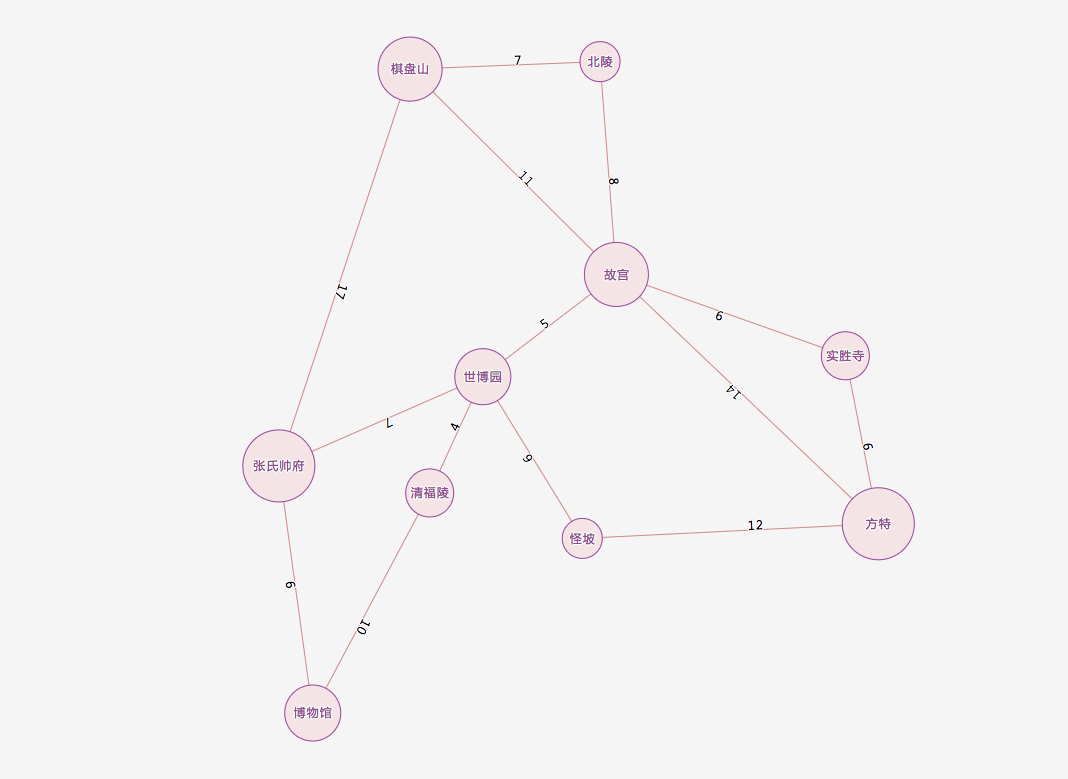
\includegraphics[width=\textwidth]{asset/54c020ae-39d8-4359-8f66-0d79cdcfc083.png}
    \caption{图论里的图}
    \label{fig:img6_2}
  \end{minipage}
  \hspace{1em}
  \begin{minipage}[h]{0.45\textwidth}
    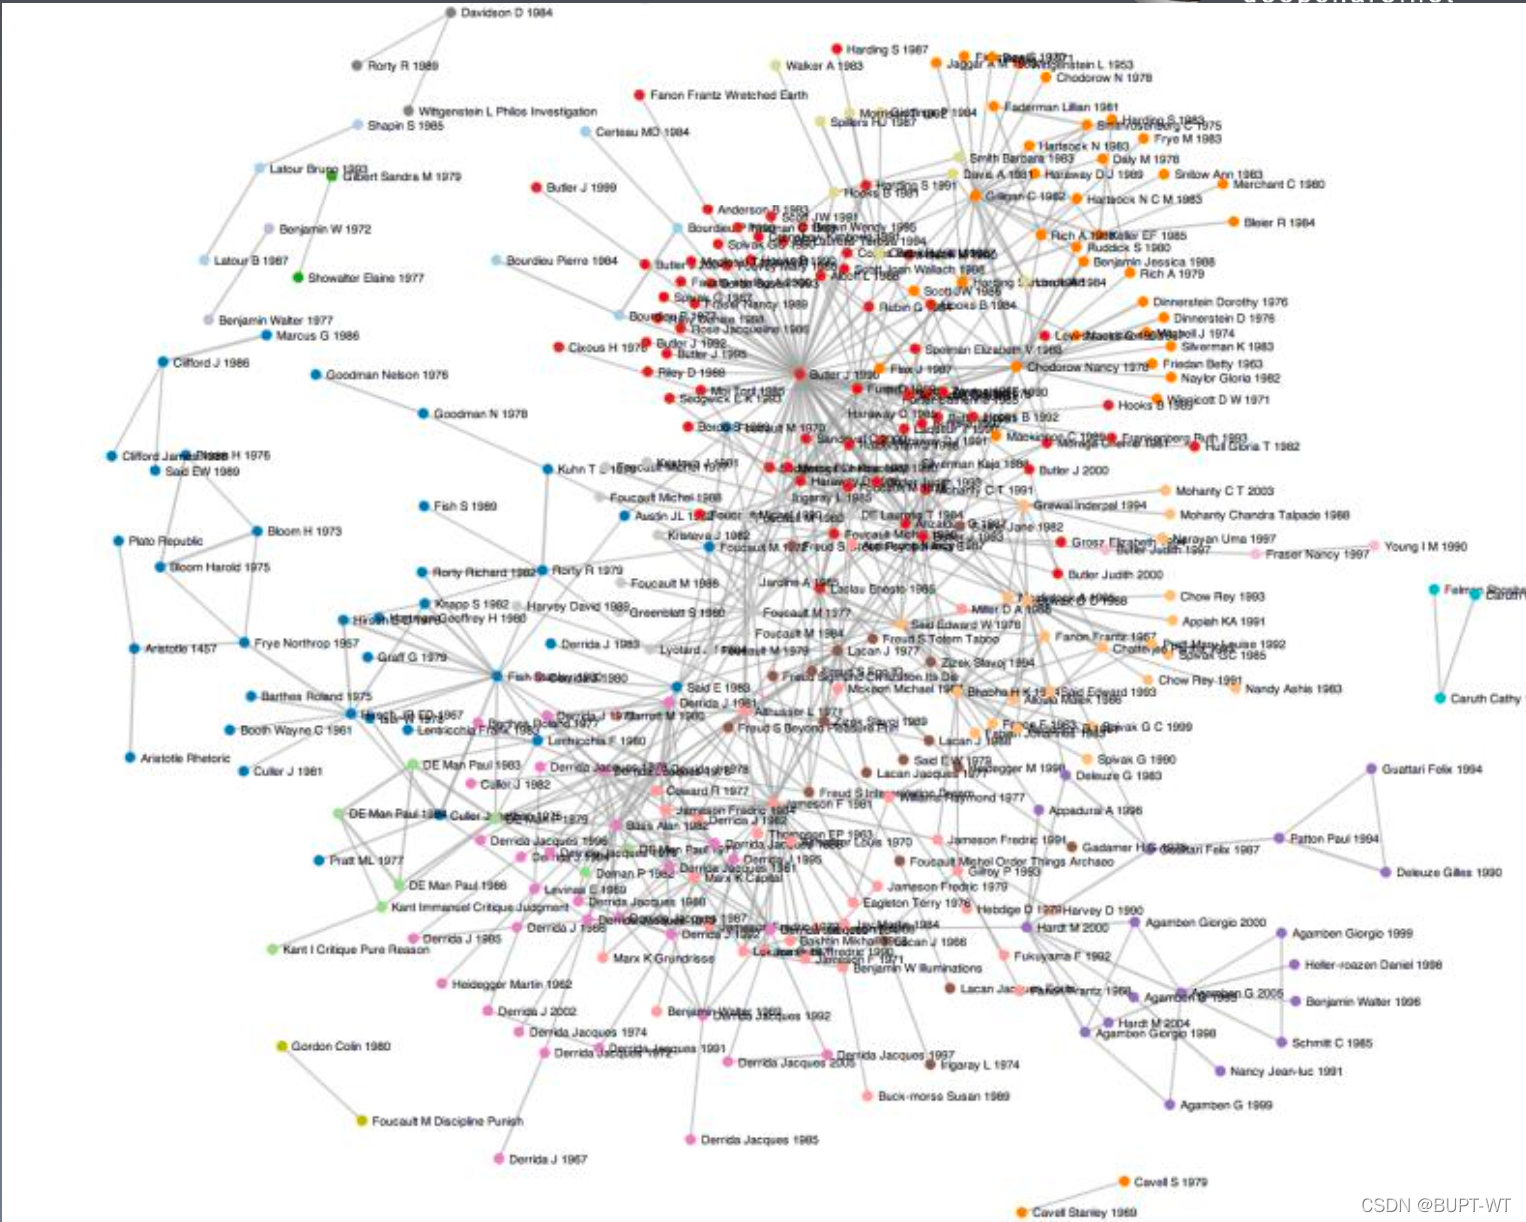
\includegraphics[width=\textwidth]{asset/2d108889-bf01-45ae-ae0c-19a3daa5a757.png}
    \caption{复杂一点的图}
    \label{fig:img6_3}
  \end{minipage}
\end{figure}

图 \ref{fig:img6_2} 就是图论里面研究的图. 它是由顶点和边构成的, 这一种网络型的结构叫做图. 当然, 复杂一点的也有, 如图 \ref{fig:img6_3}: 

所以呢, 它其实是一种抽象化的数学模型, 而不是像我们日常生活当中接触到的那样很丰富多彩, 五颜六色的. 就是一些信息量很大的点线构成网络结构. 

那为什么会有图论呢, 为什么会有人弄出这么一个很抽象的东西, 然后去去研究他呢?

图论最早的来源是柯尼斯堡七桥问题, 七桥问题我相信大家上奥数啊啥的应该都听过. 七桥问题是说, 在东普鲁士的柯尼斯堡城市里面有七座桥连接着两个小岛和河岸, 问一个人能不能从其中一个位置出发, 然后呢不重不漏的走过所有的桥, 最终回到起点, 如图 \ref{fig:img6_4}. 

\begin{figure}[ht]
  \centering
  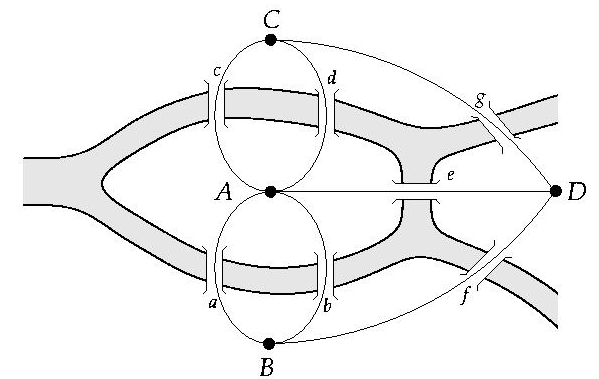
\includegraphics[width=0.7\textwidth]{asset/9d22dca2-380f-4646-8eca-179a95ce9c95.png}
  \caption{}
  \label{fig:img6_4}
\end{figure}

好多数学家, 还有数学爱好者就去研究, 就是没有人能找到走法. 后来有人把这些问题给抽象化, 用这些顶点和边来表示, 然后后来通过图论上面的方法证明出来柯尼斯堡七桥问题是无解的. 没办法从某一点不重不漏的走过任何桥然后回到顶点, 和顶点的初度入度有关了, 在这里先不展开说, 来看一下图论的概念: 

\begin{itemize}
  \item 图的构成: 顶点, 边
  \item 有向图与无向图
  \item 图的同构
  \item 边的权重
  \item 环
\end{itemize}

图的构成是什么呢?得有顶点, 有边, 顶点和边是它最基本的构成. 图还分\textit{有向图}和\textit{无向图}. 

\begin{figure}[ht]
  \centering
  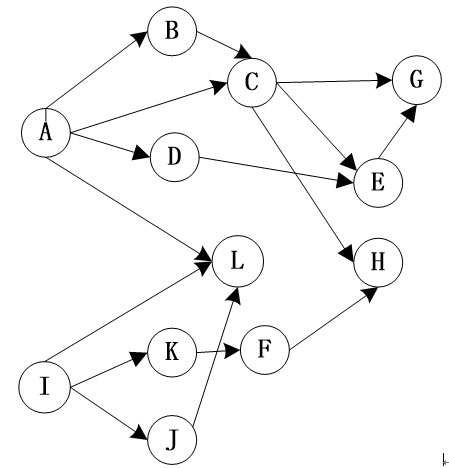
\includegraphics[width=0.5\textwidth]{asset/ee6e89d4-03e6-450b-b886-2583b91664ab.png}
  \caption{}
  \label{fig:img6_5}
\end{figure}

有向图是什么意思?就是有些边它是带方向的, 比如图\ref{fig:img6_5}中的$AD$边, 代表只能从 A 到 D, 不能从 D 到 A, 它是有向的. 而无向, 就是连接的没有箭头的边. 

图的同构是一个什么问题呢?打比方说我把 A 这一点做一个拉伸, 把 A 给拉到左边一些, 然后其他各点都保持在原地不动, 那与 A 相连的这些边是不是长度就变大了, 这样子得到一个新的图形, 和原来的图是同一个图吗? 答案是相同的图. 

所以在图论里面, 线段的长度以及顶点的大小、或者形状什么的不影响图的本质. 也就是说, 如果我们不用圆圈来表示用三角形来表示, 它还是表示同样的图. 

这就有点拓普学里面的意味了, 记得拓普学里面有个很有趣的例子: 有人问, 给你一个甜甜圈, 还给你一个碗, 还给你一个杯子. 问你杯子和碗是一类, 还是说杯子和甜甜圈是一类. 当然杯子它是一个带「把」儿的. 

就有人说, 那杯子和碗它不是挺像的吗?你把「把」儿给拿掉了, 那它不就是一样的吗?

但是按照拓普学上面的知识来说, 杯子和甜甜圈属于同一种类型, 像我们这里说的图的同构一样. 因为杯子虽然它里面是凹进去的, 但是凹进去可以再上来, 它可以进行一种揉捏的变换, 就像揉那个面团一样. 

面团可以揉下去, 也可以让他再上来对吧?做这样的变换之后会发现杯把的那个把形成的圆环其实是和甜甜圈是一样的. 甜甜圈有个环对吧?杯子的把也是有个环. 杯的深度可以通过伸缩变成一个实心的, 凹下去就没有内容的空间了. 但是形成的环, 是没办法给它去掉的. 所以, 这就是图的一个同构. 

然后我们再来说一下边的权重. 

各个边可能会有一些数值, 代表了权重. 我们在路径规划的时候, 权重可以代表什么呢?比如说 A 到 B, 这里标一个 10, 代表 A 和 B 之间, 它边的权重 10, 物理意义就是它的距离为 10 公里. 

权重可以赋予一些物理意义, 比如刚才说的路径. 最短路径的规划, 就必须对边有个权重的分配. 权重还可以表示其他的一些物理意义. 总之相当于给边赋予一个数值. 

环是什么意思呢?假设, 这里我们先不看这些箭头和这些 ABC 点, 它是不是就形成了一个闭环?在图里面它形成了一个闭环, 而这种结构就叫做就叫做环. 

主要带大家了解一下概念性的东西, 对应的图、文字描述, 如果有忘记的地方再重新看一下就行. 因为图论相对于前三个部分在人工智能里面用的场景相对比较有限. 

图论与 AI 它有什么样的关系呢?

一个就是最短路径的搜索, 边有权重之后可以根据权重值决定最短路径是怎么样的. 

还有推荐系统, 拿亚马逊或者京东打比方. 它会把你点击的这些商品用图的结构给连接在一起, 然后用图论的方式去处理, 看下一次给你推荐什么样的东西\footnote{关于推荐系统,咱们「BI 篇」里有详细的讲解,敬请期待。}. 还有包括像 Facebook、微信这种社交网络的分析, 用户与用户之间形成的结构也是图的结构. 

\hypertarget{数学如何运用于 AI}{}
\section{导论总结: 数学如何运用于 AI}

接下来我们来总结一下当前所讲的这些课. 

这几节课的总体概念都是基础, 是帮大家回忆一下相关数学知识, 或者说是帮大家了解一下. 

这些数学知识如何运用于 AI? 之前的课程中说过: 

\textbf{导数} 就是用于反向传播. 要优化损失函数必须对他进行求导, 在神经网络里面要把导数一层一层的从后往前传. 

\textbf{矩阵} 就是 AI 模型里面基本的数据结构以及参数结构. 不管是神经网络层, 还是神经网络接收的数据类型, 都是以矩阵、或者说向量的形式存在的. 

\textbf{概率统计} 应用的比较多, 在机器学习里面它也有一个统计学派叫做统计学习. 我相信大家都听说过李航的那本《统计学习方法》, 他就是以统计学的方法为一个基准点, 研究机器学习的一些方法. 里面包括一些贝叶斯分类、最大自然估计这些. 我们之后也会挑一些重点给大家讲解. 

\textbf{图论} 应用的主要是概率图的模型. 比如说大家可能听过的 BS 网络, 还有马尔科夫网络. 当然还有其他一些知识也会用于 AI, 在之后的课程会学习到. 

之后的课程里会仔细讲解 AI 中会用到的这四个知识点, 下节课我们会从导数开始, 希望让大家以最短的学习路径学到自己需要的知识, 将来能为自己的工作所用, 提高大家的\textbf{工作能力}或者\textbf{工资上限}. 
% \chapter{函数}

\begin{figure}[ht]
  \centering
  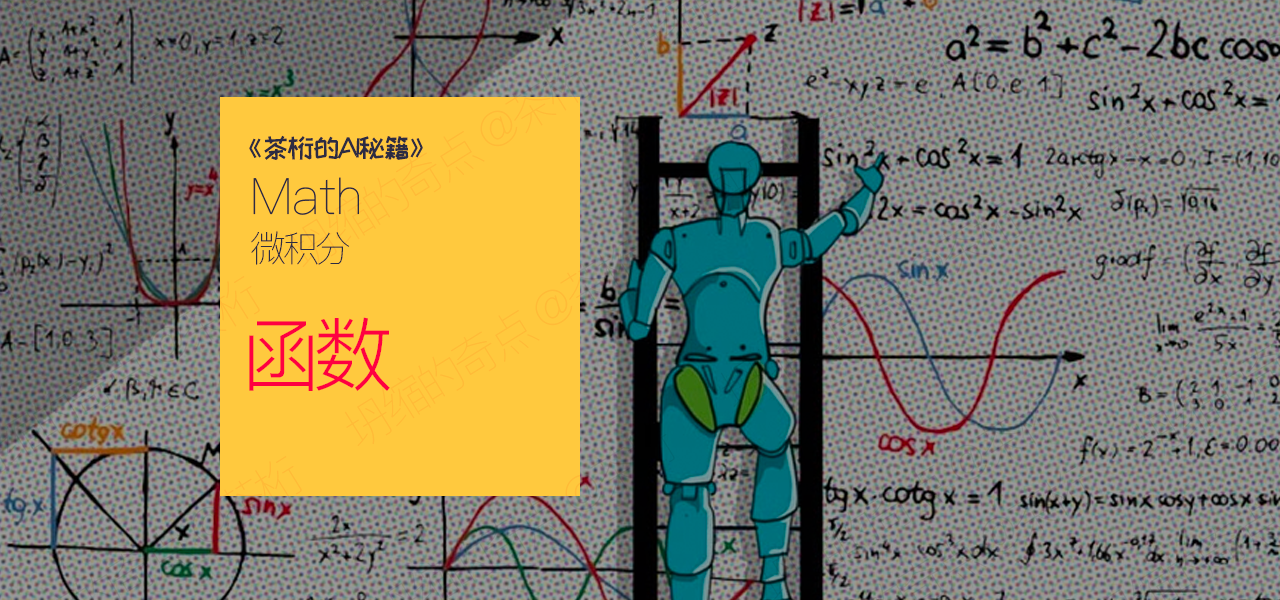
\includegraphics[width=1\textwidth]{asset/茶桁的AI秘籍_Math_6.png}
\end{figure}

\newpage

经历了前面5节课的基础之后, 不知道大家感觉怎么样?我后台接收到了一些反馈, 有的同学说比较简单; 有的同学说正合适; 有的同学就觉得有些绕, 一时之间可能没办法理解和接受. 说明同学们的水平还是有一些参差不齐的. 

其实每个人的背景都是很不一样的, 大家的方向也各有不同. 有CV方向, 有NLP的, 还有Data Science的. 可是也有很大一部分小伙伴也许就是零基础想要进行转行, 进入赛道. 

可是我也只能写这么一份, 会尽量照顾到大部分人, 可能会针对初学者而言比较友好一点. 咱们不可能真把这几节课当成是数学系的同学专研的那种. 那么对于基础有些过分薄弱的, 希望同学们课下能多发挥一下自主学习的能力, 躲在其他地方进行一下补足. 咱们这节数学课虽然比较偏基础, 但也并不可能一点难度没有. 所以基础太过薄弱的同学, 课下稍微去努努力, 夯实一下自己的数学底子. 

咱们AI秘籍的课程, 以后也会有很多时候是需要自己去不断练习, 发现问题解决问题. 那同学们必须学会自己去自主学习. 咱们的课程就只是将最主要的知识点讲给大家, 带大家一程. 更重要的是你要学会如何自己解决问题. 有问题的, 可以后台留言问我, 但是你指望我手把手带那就有点不太现实了. 如果你之后进入了这一行, 或者说不管你做哪一行, 工作的时候指望着有一个人手把手的教你那肯定是不可能的对吧?领导看到你这样的话肯定很生气, 到了年底的时候也许给你末位淘汰. 所以还是希望大家自己能发现问题, 并且自己知道如何去解决问题. 

好了, 话不多说, 我们开始今天的课程. 今天开始, 之后的几节课都是关于\textit{微积分}. 

微积分是我们在数学领域很重要的一个部分, 我们在之前的基础部分里面已经说过AI方面\hyperlink{数学如何运用于AI}{需要哪一些数学知识}, 第一个就是微积分. 当然其他还有线性代数、概率统计、图论这些. 

\hypertarget{6.微积分-函数}{}
\section{函数}

我们开始的第一个内容, 就是函数. 在基础课里面说过, 函数是有很多种不同样的形状的. 可以是一元, 也可以是多元的. 就比如说一次函数、二次函数、正旋、以及指数函数、对数函数. 

\begin{align*}
  & y = x + 1 & y = x^2 \\
  & y = sinx & y = e^x \\  
  & y = log_2^x & z = x^2 + y^2 \\ 
  & ...
\end{align*}

函数包括的种类其实非常多, 化成的函数图像也是非常的多样性. 各个函数对应的函数关系不一样. 比如图\ref{fig:img7_1}右下角的那个图形, 就是二元函数的图像. 其中X、Y是作为自变量, Z是在XY的基础之上去构建的一个三维的图形. 

\begin{figure}[ht]
  \centering
  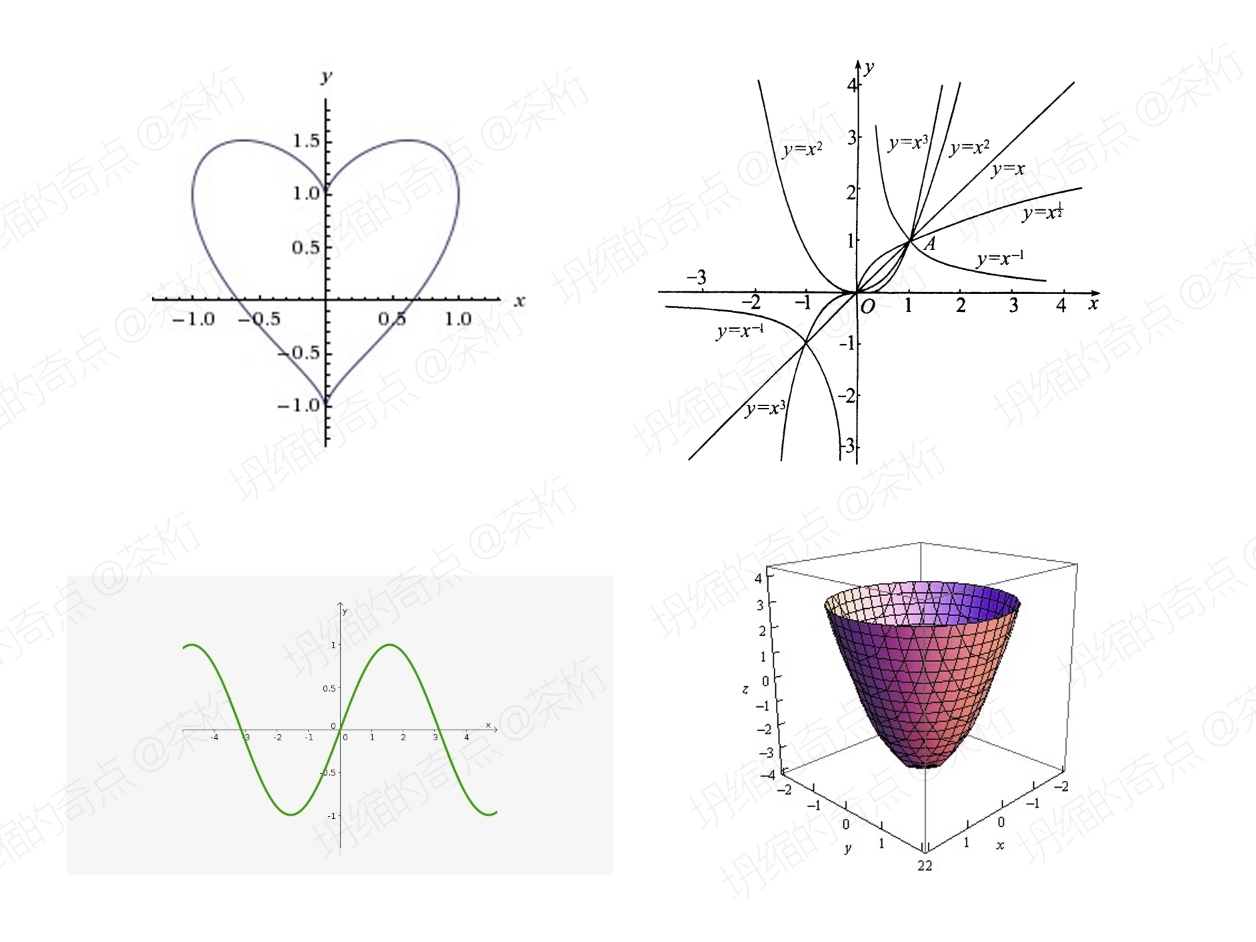
\includegraphics[width=1\textwidth]{asset/0c36f8c5-0b4f-4fc1-a5dc-a206fd7e2db2.png}
  \caption{不同的函数图形}
  \label{fig:img7_1}
\end{figure}

看了之前课程的小伙伴应该还记得, 左上角的那个图像其实它不是函数的图像. 因为它一个X对应的两个Y值, 

从本质上面来说, 如果我们抽象一点, 函数它其实是从一个集合到另外一个集合的一种映射规则: $f:R -> R$.

这么说可能会有点抽象, 集合和映射规则什么意思?这里的集合就和我们日常生活当中理解的集合差不多. 就是一堆东西, 然后把它们聚在一起形成的一个聚合体, 我们把它叫做集合. 

在数学上面的集合可以理解为一个数的集合, 数的一个聚合体. 

所以函数其实就是给你一个集合, 然后再给你一个映射规则. 规则可以把集合里面的每一个数给映射到另外一个集合里面. 

就是在映射规则之下, 右边的集合里面有一个数会和左边里面的数一一对应. 

R在数学上表示实数集. 实数、虚数、负数大家应该有听过吧?即便没学过的同学应该有听过. 实数就是我们在自然界当中可以接触到的实际存在的这些数字, 比如说你的身高多少, 世界上有多少个国家, 这些东西都是有实际意义的. 

虚数是什么呢?比如-1的平方根 $\sqrt{-1}$, 按照实数的理解来说它是不存在的. 那任何数的平方就是自己乘自己, 它肯定是一个非负数, 怎么可能是-1呢?但是在数学上面它确实存在, 我们在现实生活当中可能不太会遇到. 

函数之前讲过, 是从一个集合到另外一个集合的一种映射规则. 就像是你把你的手放在蜡烛前面, 蜡烛就会通过光把你手形成的影子投在墙壁上. 那手和墙上的影子就是类似于这么一种映射规则. 

函数可以是很天然的, 比如:

\begin{align*}
  y & = e^x; \\
  y & = sinx;
\end{align*}

这两个式子中, 咱们先来看$y=e^x$, e叫自然对数, 就有点像是生物物种不受任何限制的去增长, 它的种群数量会是一个爆炸式的增长. 就可以用$y=e^x$来表示. 

$y=sinx$, 是正弦. 在发电站里面发的交流电就是这种正弦波的形式, 也是来自于自然的. 

当然也可以人工去创造一些函数. 比如迪利克雷函数非常有意思. 当X是有理数的时候, 函数值是1, X是无理数, 函数值是0. 

看到这里先停下思考下, 你觉得迪利克雷函数的图像应该长成什么样子? 我在这里做了一个刻意的排版,将图放在了下一页。大家先畅想一下, 不要急着往下看, 给自己一点时间想想, 按照这种规则, 吉利克雷函数的图像应该长成什么样?

\begin{align*}
  f(x) = 
  \begin{cases}
    1, \qquad  x \mbox{是有理数} \\
    0, \qquad  x \mbox{是无理数}
  \end{cases}
\end{align*}

如果在不考虑到精确度的情况下, 我们可以把它的函数图像画成图\ref{fig:img7_2}的样子. 

我们来看, 上下各有一条平行线对吧?肉眼看上去上下是一条平行线, 但其实图像只是看似连续的, 实际上这些线并不是连续的, 是无限多个点. 

\begin{figure}[ht]
  \centering
  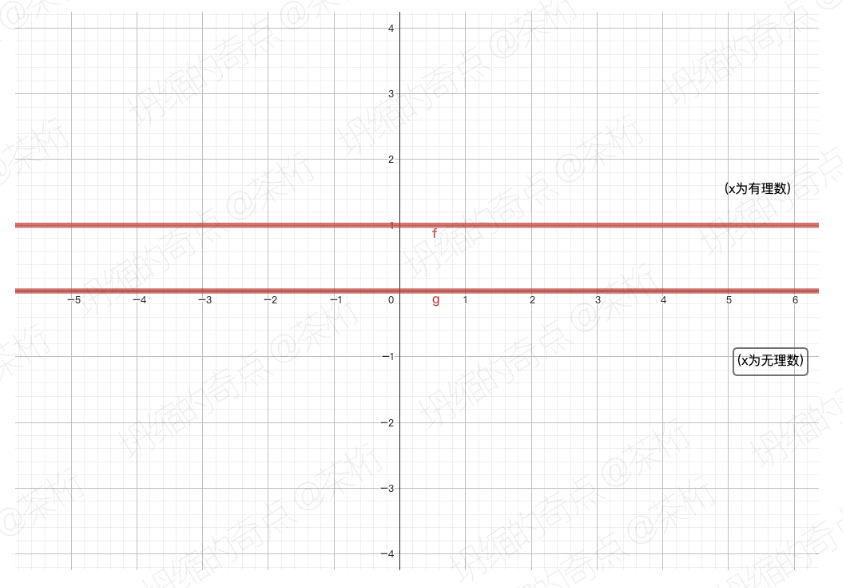
\includegraphics[width=0.8\textwidth]{asset/97060faa-bcf8-4fdb-8f69-e42425ab9575.png}
  \caption{迪利克雷函数的图像}
  \label{fig:img7_2}
\end{figure}

因为实数有个稠密性, 就是说有理数也是无限多的, 无理数也是无限多的. 在任意小的一个区间之内, 他俩都是无限多的, 那些断点你肉眼看不着. 所以, 其实\textbf{迪利克雷函数虽然是客观存在的, 但是我们无法画出来}. 上面图像只是一个近似. 

现在我们知道, 函数抽象来说是一个什么样的东西: 是一种映射的法则. 那我们应该怎么样去表示它呢?

首先很熟悉的, 我们知道可以用解析式去表示. 一个自变量X、一个因变量Y, 他们之间的一种数量关系. 

解析式: \(y = e^x\)

还有可以通过文字描述的形式, 就像迪丽克雷函数: \textit{自变量为无理数时因变量取值0, 有理数时取值1}. 一般都是通过这种方式去描述它. 

然后还有一种, 叫做列表法. 列表法就是把自变量值和应变量的值给它一一对应起来, 也可以代表一种映射规则. 

\begin{table}[ht]
  \centering
  \begin{tabular}{llllll}
    \midrule
      x & 1 & 2 & 3 & 4 & ... \\
      y & 2 & 4 & 6 & 8 & ... \\
    \bottomrule
  \end{tabular}
  \caption{列表法}
  \label{tab:table7_1}
\end{table}

结合刚才所说的这些内容总结一下, 函数主要包含三个部分:

\begin{itemize}
  \item 一个是定义域(整数域, 实数域, 复数域...)
  \item 一个值域(整数域, 实数域, 复数域...)
  \item 还有个映射法则(将定义域映射到值域)
\end{itemize}

映射法则就是作用在定义域上面, 把定义域里面的数给映射到值域上面. 结合我们手投影在墙上的例子来看, 把手比作定义域, 蜡烛可以看作映射法则. 蜡烛的光照在定义域上面, 就形成了墙上的影子, 就是值域. 

但是, 不是所有的映射法则都可以构成函数. 对于函数有一个比较严格的要求, 就是一个自变量在值域当中有且只能有一个因变量与它相对应. 如图 \ref{fig:img7_3}:

\begin{figure}[ht]
  \centering
  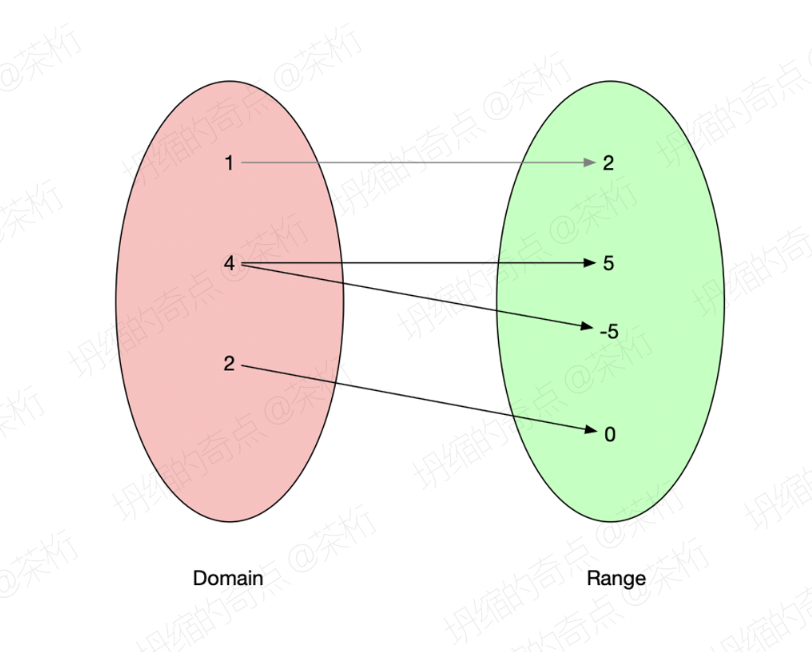
\includegraphics[width=0.55\textwidth]{asset/78b109d0-c39f-446b-ba0a-2b983138d76f.png}
  \caption{}
  \label{fig:img7_3}
\end{figure}

途中左边集合是定义域, 就是我们的手; 右边的集合就是墙上的影子. 我们会发现在映射规则之下, 数字4被映射到了值域里面的两个值上面. 是不可能的, 就像光照到你大拇指, 投在墙上只可能形成一个大拇指的影子, 不可能同时显出两个大拇指的影子. 除非有两个映射规则, 也就是有两个蜡烛. 所以这种映射规则就不能称作为函数. 

对于函数这部分的理解, 也差不多就讲到这里了. 大家只要把握住它是一种映射规则. 其实说白了就是一种转换规则. 然后, 它是作用于定义域的, 定义域的数在映射法则或者说转换法则的作用下映射到了值域上, 就是做了一种转换. 
% \chapter{极限}

\begin{figure}[ht]
  \centering
  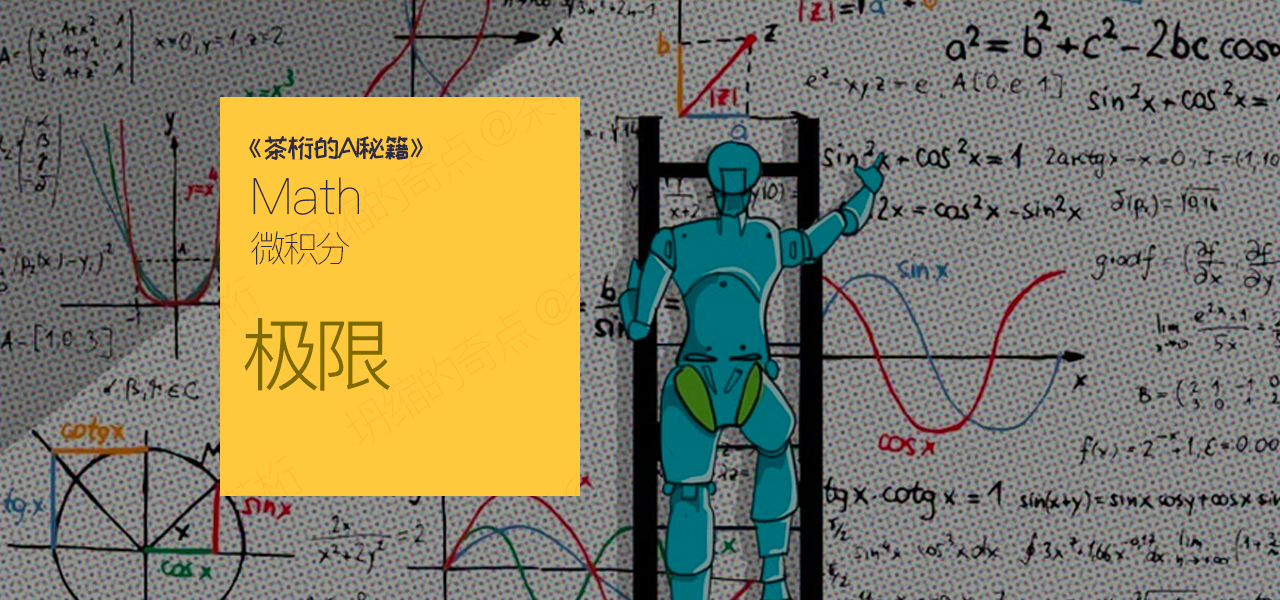
\includegraphics[width=1\textwidth]{asset/20230827220554.png}
\end{figure}

\newpage

今天的课程还是微积分系列课程中的一节. 上一节课我们详细介绍了一下函数, 给大家解释了函数的本质. 这节课我们要来讲一下微积分里的另外一个概念: 极限. 

在这节课中, 我们会看到一些公式, 我还会带着大家推导一些东西. 

\section{极限}

首先说一下极限这个概念. 

极限这个词我们已经听过很多次了, 就是什么趋近什么的极限, 在这个点的附近极限等于多少多少. 大家都听过很多诸如此类的这种描述. 

那我们怎么样从数学的角度去严谨严密的描述极限是怎么一回事呢?什么样才叫无限逼近某一个量?以及这个量可以到达吗?也就是说, 极限我可以取到吗?还是说我永远只能逼近他, 却永远达不到. 这听着就感觉有点伤感, 就像一个男生追一个女生永远追不到.

首先来看一下极限正式的定义: 

\begin{newquotation}
  设函数$f(x)$在点$x_0$附近有定义, 如果存在常数$a$, 对于任意给定的正数$\varepsilon$, 都存在正数$\delta$, 使得对于任意$x$满足$0<|x-x_0| < \delta$, 均有$|f(x)-a| < \varepsilon$, 则称常数$a$为$f(x)$在$x$趋近于$x_0$时的极限, 记作: 
  \begin{align*}
    \lim_{x-x_0}f(x) = a
  \end{align*}
\end{newquotation}

以上定义是一段极限的标准定义, 对于极限除了标准定义之外还有「左极限」和「右极限」这两个概念, 分别为 左极限: $\lim_{x-x_0^{-0}}$, 右极限:$\lim_{x-x_0^{+0}}$. 不过对比下来发现, 其实我们平时所求的极限, 本质上都是先求了左右极限, 然后二者相等, 才得到了我们的函数极限. 也就是说, 如果左右极限不相等, 那么函数在这个点上极限不存在. 而且平时我们也很少先求左右极限再比较得到极限. 

还是来继续讲解极限. 我们先用一段非常数学化的语言去描述一下极限正式定义: 设有一个函数$f(x)$在点$x_0$附近有定义, 「有定义」就是$f(x)$在$x_0$附近都可以映射. 如果存在一个常数$a$满足下面的条件, 任意给一个正数$\varepsilon$, 不管这个正数多大还是多小, 只要是任意的, 都存在另外一个数$\delta$, 并且也是一个正数, 使得$|f(x)-a|<\varepsilon$. 就是$f(x)$和$a$相减的绝对值小于$\varepsilon$小于你任意给的这个数$\varepsilon$这个结论在$|x-x_0|$属于$(0, \delta)$ 这个区间之内的时候恒成立. 如果这样的话, 我们就把常数$a$称为$f(x)$在趋近于$x_0$时的极限. 

不要发懵, 我们来详细解释一下. 

首先来看$x_0$附近的定义, 所谓$x_0$附近, 实际上就是指一个以$x_0$为中心的「去心邻域」. 

那什么是「去心邻域」呢?我们来拿一个数列说明一下: 

\begin{align*}
  [-5,-4,-3,-2,-1,0,1,2,3,4,5]
\end{align*}

在这一组数列中, 假设0就是$x_0$, 那么这整个数列就都是$x_0$的邻域. 如果关心它的半径, 这段去心邻域的半径就是5. 因为现在给定的是一个确定的数列所以半径我们知道, 但是大部分时候我们并不知道这个$x_0$的邻域是多少, 所以可以用$\delta$来替代, 也就写成$(x_0, \delta)$, 这个$\delta$当前并不是在这个数列中的任意值, 而是一个半径值. 如果用图像表示, 可以表示为图\ref{fig:img8_1}这样: 

\begin{figure}[ht]
  \centering
  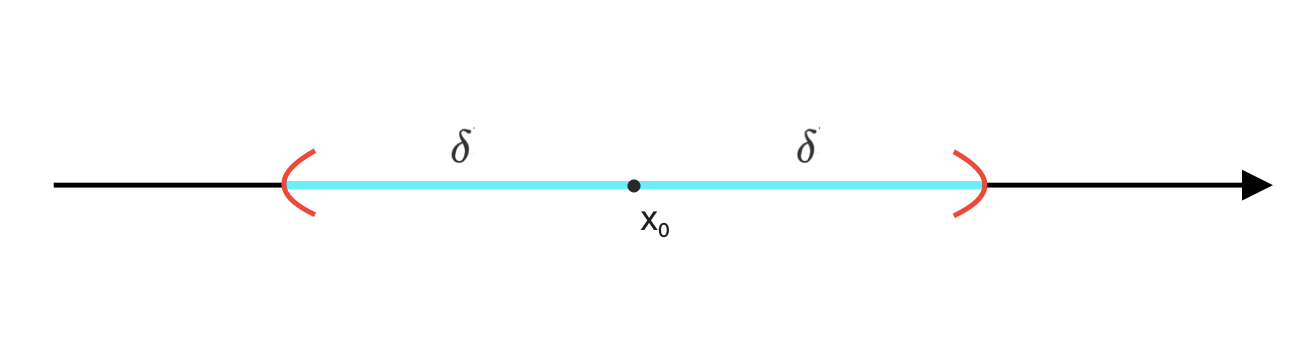
\includegraphics[width=1\textwidth]{asset/c1569200-3866-4cf7-8ec1-6cc23521eaff.png}
  \caption{$x_0$及其邻域}
  \label{fig:img8_1}
\end{figure}

那在这个图像中如果去掉$x_0$这个中心点, 就是$x_0$的去心邻域, 也就是定义里的「$x_0$ 附近」. 

之前已经说了, 在点$x_0$的附近这个函数都可以映射, 这些点就相当于$x_0$附近的这些点. 都是我们的手, 这些蜡烛的光都可以照到, 函数的规则都可以映射到. 

$\varepsilon$是任意给定的, 无论这个$\varepsilon$多么小, 小到令人发指的程度, 如果存在常数$a$, 求$|f(x)-a| < \varepsilon$都能成立. 

只需要一个条件, 就是先找到一个正数$\delta$. $|x-x_0|$ 是在$(0,\delta)$ 这个区间范围内. 这个区间范围内就是 $0<|x-x_0|<\delta$, 一个开区间\footnote{开区间, 高一知识点. 开区间用圆括号表示, 表示这个端点取不到. 如果是用方括号来表示, 就表示端点值可以取到, 那就是闭区间.}. 我们之前已经说过了, $\delta$是一个半径取值, 从理论上来说, $\delta$是不可能为负数的. 

所以只要我能找到这么一个正数$\delta$, $|x-x_0|$ 在 $(0, \delta)$ 范围之内不管$\varepsilon$有多么小都可以满足$|f(x) - a| < \varepsilon$. 那我们就可以得到这样的结论:$\lim_{x-x_0}f(x) = a$, 我们就说$f(x)$它在$x$趋近于$x_0$的时候极限为$a$, 这个常数$a$就是这个函数在这一点的极限.

在这个定义中, $x_0$和常数$a$都类似于基准点, 而$\delta$和$\varepsilon$都类似于精度. 这个定义的意思是, 给定任何一个需要达到的精度$\varepsilon$(即$|f(x)-a|$)都能找到一个$\delta$, 使得在$x_0$去心邻域这么小的范围内, $f(x)$均在$\varepsilon$精度内. 也就是说, 当不断缩小$f(x)$的范围的时候, 总能通过缩小$x$的范围, 使得$f(x)$落在给定的范围内. 

这个是比较绕的. 下面我带大家先看一下这个例子, 如果大家一时还看不太懂没有关系, 也不要慌, 先来看一个简单一点的: 

\begin{align*}
  x\in [-1, 1], \lim_{x \to 0} x = ?
\end{align*}

那这个式子里,这个函数y就等于x, 我们弄一个最简单一个函数. 先告诉你这x的取值范围是[-1,1], 就是说, 我们手的范围就是这么大, 这个蜡烛的光只能照到这个范围. -2照不照得到呢?照不到,那2照不照得到呢, 也照不到. 然后我们考虑当$x$趋向于0的时候($x\to0$), 这个式子的极限是多少.

首先大家可以看一下. 从直觉上面判断既然$x$可以取到0了, 这个0不就是在-1到1之间吗?所以既然能取到逼近他的时候, 这极限的趋势当然就是0了. 

那我们接下来再看第二个: 

\begin{align*}
  x \in [-1,0) \cup (0, 1], \lim_{x \to 0} x = ?
\end{align*}

那这个式子里, 我们把0给去掉了. 这个$\cup$符号呢叫做并集,表示把这两个集合或者说区间给它并在一起. 并在一起之后这两个就都是我们手的范围了. 

那现在问题来了,0现在取不到了, 不属于这个区间. 那我这个时候$x$的极限在这一点会是什么样的情况呢?

首先,我们先猜想一下它的极限值为$a=0$, 别急, 我们只是先猜想一下. 然后按照这个定义我们任意取一个$\varepsilon$, 任取一个, 随便怎么取都行. 然后我们令$\delta$等于$\frac{\varepsilon}{2}$, 这个是符合我们定义的, $\varepsilon$是任意的,$\delta$是可以自己取, 因为定义里面$\delta$只要存在一个就行了, 只要能找着. 

那你就可以自己去添加一些性质, $\delta = \frac{\varepsilon}{2}$, 这个当然也是大于0的, 所以我们来看一步步的, 严格按照极限的这个定义来看的话, 当$|x-x_0|$落在了大于0,小于$\delta$这个范围之内. 

\begin{align*}
  0 < |x-x_0| < \delta
\end{align*}

我来解释一下, 为什么要让这个绝对值大于0呢?为什么不能等于0呢?等于0其实对应的什么样的情况, 就是$x=x_0$. 如果它们相等, 就跟我们刚才第一个式子里一样了, 都可以取到. 那你这时候来讨论极限就没什么意思了. 大家都知道1+1=2,现在拿这个考大学生没什么意思了对吧?

所以我们把这个等于给它去掉, 让它大于0, 小于$\delta$这个范围. 我们把$\delta$再换一下, 用$\delta = \frac{\varepsilon}{2}$这个式子再换一下, 它就变成了这么一个式子: 

\begin{align*}
  0 < |x - 0| < \frac{\varepsilon}{2} \\
\end{align*}

好,那我们再来看一下: 

\begin{align*}
  |f(x)-a| = |x - 0| < \frac{\varepsilon}{2} < \varepsilon
\end{align*}


这时候$f(x)-a$不就是$x-0$么?$f(x)$就是$x$, a我们假设它就是0. 所以在这里我们得到的$|x-0|$, 其实不就是上面式子$0<|x-0|<\frac{\varepsilon}{2}$中的$|x-0|$吗? 我们已经知道它是小于$\frac{\varepsilon}{2}$的, 那它肯定是小于$\varepsilon$. 所以就证明出来, 只要$|x-x_0|$在$(0, \varepsilon)$这个范围内, 这个函数$f(x)$减去它的极限$a$就小于$\varepsilon$. 就证明出来了它的极限值确实是0. 

\begin{align*}
  \lim_{x \to 0} x = 0
\end{align*}

那我下面呢,就给大家一个完整的求值过程: 

\begin{align*}
  & x \in [-1,0) \cup (0, 1], \lim_{x \to 0} x = ? \\
  & \mbox{解:  (按照极限定义)}\\
  & \mbox{猜想其极限值为}a = 0, \mbox{取任意}\varepsilon > 0, \mbox{令} \delta = \frac{\varepsilon}{2} > 0 \\
  & \mbox{则,当} 0 < |x-x_0| < \delta, \mbox{即} 0<|x-0| < \frac{\varepsilon}{2} \mbox{时},\\
  & |f(x) - a| = |x - 0| < \frac{\varepsilon}{2} < \varepsilon \\
  & \mbox{所以} \lim_{x \to 0} x = 0
\end{align*}

看到这里, 有些小伙伴可能会比较懵. 其实这一部分如果实在理解不了, 也可以暂时先放在一边不用去管它. 我们知道极限是一个什么样的东西就可以了: \textit{它代表一种无限逼近的一个过程}. 知道这点, 就OK了. 至于这个理论推导, 包括证明, 其实大家不用太care它. 

整个证明的过程, 其实核心思想就是$\varepsilon$得是任意的,$\varepsilon$控制不了.  别人给你一个$\varepsilon$, 不管什么$\varepsilon$, 都得满足这个上面的式子. 

所以, 我们在证明过程中, 取值用了一个词「任意」.  用「任意」去表示它. 但是在$\delta$这里, 为什么我们可以令它是$\frac{\varepsilon}{2}$,其实我们在这里令它是$\frac{\varepsilon}{3}$、$\frac{\varepsilon}{4}$, 甚至其他什么式子都可以, 没有关系. 因为定义里面说了, 虽然$\varepsilon$是任意给的控制不了, 但是这个$\delta$只要能找到这么一个, 哪怕只能找到一个,它是一个正数, 使得$|x-x_0|$落在$(0,\delta)$这个范围之内就能推导出$|f(x) - a| = |x - 0| < \frac{\varepsilon}{2} < \varepsilon$. 如果能找到这样的$\delta$就可以说它的极限等于啥啥啥. 

所以我们比较能操作的部分就在于这个$\delta$的选取,这个选取可以自由发挥. 当然了,最终的目的还是在倒数第二步里, 能用关系推导出来$|f(x)-1| < \varepsilon$就可以了. 

整个过程似乎看着很随意是吧?随便弄了一个$\delta$, 然后就\textit{kua kua kua}写式子, 就证明出来相等了, 这样感觉好像不对. 

那我们就来看一个反例, 来说一下为什么上面这个极限表达的极限不是0.1. 

\begin{align*}
  & x \in [-1,0) \cup (0, 1], \lim_{x \to 0} x = ? \\
  & \mbox{思考:  为什么0.1不是其极限值?}\\
  & \mbox{假设其极限值为}a = 0.1, \mbox{取} \varepsilon = 0.05, \mbox{对任意}\delta > 0, \\
  & \mbox{则当} 0< |x-x_0| < min\{\delta, \varepsilon \}, \mbox{即}|x-0| \in (0, 0.05)\mbox{时} \\
  & \mbox{有}-0.05 < x < 0, \mbox{或} 0 < x < 0.05 \mbox{时} \\
  & |f(x)-a| = |x-0.1| \in (0.05, 0.15) \Rightarrow |x-0.1| > 0.05 = \varepsilon \\
  & \mbox{所以} \lim_{x \to 0} x \ne 0.1
\end{align*}

我们先用反正法来来看一下, 先假设它就等于0.1. 这时候取$\varepsilon = 0.05$, 对任意$\delta > 0$. 大家看到这里可能会迷糊, 刚才那个证明里面不是说$\varepsilon$是别人强塞给你的, 任意的, 别人给啥你都得接受吗? 那怎么这里$\varepsilon$可以自己取了? 刚才$\delta$不是可以自己取的吗, 怎么现在$\delta$控制不了, 得是任意的, 别人强塞给你什么你都得接受了?

这个, 涉及到命题里面的的「否命题」这么一个概念. 命题逻辑这部分知识说如果我们把一个命题取否的话, 那原来它那个文字表述里面写着任意两个字的地方全部要改成存在. 原来存在的地方都要改成任意, 这是一种相互对称的关系. 我鼓励大家自己去搜一下, 命题的否定, 否命题. 

因为我们要证明它不是一个极限, 所以这里就和刚才反着来, $\varepsilon$随便找一个, 任意的$\delta$大于0,当我这个$|x-x_0|$处于$ 0< |x-x_0| < min\{\delta, \varepsilon \}$范围之内的时候. 

接下来这里可能又有点迷糊人,$min\{\delta, \varepsilon\}$嘛意思, 这个式子表示什么? 这个花括号里面组成了一个集合, $min$表示我取这个集合里面的最小值. 在这里就表示在这两个数里面取一个最小值的意思. 

那为什么要添加这个东西呢? 这也是一个比较困难的地方, 就是$\delta$确实是任意的, 别人强制性塞给我, 我必须得接受的. 但是我可以同样采取一个比较巧妙的一个措施. 的确这个$\delta$扔给我之后, 其实我们真正关心的是$x$和$x_0$非常接近的情况. 因为当$x$和$x_0$差很多的时候, 极限肯定也差的很多. 

就像图像上面两个点,连续函数图像,如果两个点差的特别远,那他们的函数值肯定也会差的比较远. 但是如果两个点挨的比较近,那函数值也比较接近. 

所以虽然$\delta > 0$, 但其实我们认为真正有用的部分是$\delta$非常非常小的时候. 所以在这里弄一个$min$,就控制了$\delta$再大,至少通过这个操作也让这个$x-x_0$的这个范围限定在0.05,也就是$\varepsilon$这个值. $\delta$取20也没什么意义. 那取小一点, 就按照$\varepsilon$来. 

如果$\delta$本身就非常小, 比如说取值0.01, 这个时候0.01是小于0.05的. 那我就取0.01. 所以就是谁小谁厉害. 

在这因为我们真正关心的是$|x-x_0|$非常接近的时候, 也就是他们的差非常小的时候.不管最终$min$取出来是$\delta$还是$\varepsilon$, 也不管这两个都是什么值, 我们都一定有$|x-x_0|$, 也就是后面的$|x-0|$, 它是属于$(0, 0.05)$这个范围的. 

$\delta$取值20的时候, 那取值范围就是(0, 0.05), $\delta$取值0.01的时候,那取值就是(0, 0.01). 不管怎么样,肯定是要属于这个集合或者他的子集. 那我们就能把这个绝对值拆开, 拆成$-0.05 < x <  0$和$0<x<0.05$ 这两个. 拆绝对值这里大家应该都懂吧? $0< |x| < 0.05$, 所以拆出来是这两个范围. 

拆出来之后,我们再来看一下最后这一步. $|f(x)-a|$ , a是一个假设值, 所以$|x=0.1$ 属于$(0.05, 0.15)$这个范围. 通过计算$|x-0.1| > 0.05$. 当$|x-0.1|$属于这个范围的时候, 代表着$|x-0.1|$ 是大于0.05, 小于0.15的. 也就是$0.05 < |x-0.1| < 0.15$, 小于0.15我们不关心, 我们就关心这个0.05. 那取值大于0.05, 那就等于是大于了$\varepsilon$. 因为0.05就是$\varepsilon$. 所以我们就发现, 极限值$a=0.1$, 但是我能找到这么一个$\varepsilon$, 当$\delta$取任意值, $|x-x_0|$满足这个条件的时候,  函数值减去假设的极限得出来的结果竟然是大于$\varepsilon$的. 所以这个就不符合极限定义了. 

按照极限定义肯定是要小于它, 结果现在是大于. 所以它的极限就不是0.1. 

我知道, 很多人读到这里一定是一脸懵逼. 也没有关系, 尤其是对数学底子比较薄弱的同学啊, 我相信肯定会有人懵逼, 你可以把这一块先放一下.

我们之后做AI的时候不仅仅只是做编程, 不仅仅是敲代码. 用Tensorflow、用PyTorch、去敲代码. 以后在职场上面需要往上晋升, 要提升自己能力的时候, 你还是需要结合一点数学的. 如果没有这个数学思想去给你探路的话, 你很难有一个非常广阔的一个提升空间. 

我知道可能很多人已经很多年没接触数学这个东西了, 而且在这里这么短的篇幅想要讲完这些东西强度肯定比较大. 看不懂的可以多看几遍,对着我的解释和公式一步一步推敲. 

在以后, 我计划着如果有时间的话, 给大家录制相关的教学视频, 对照着视频动画来看可能会理解的更加通透一点. 
% \chapter{连续}

\begin{figure}[ht]
  \centering
  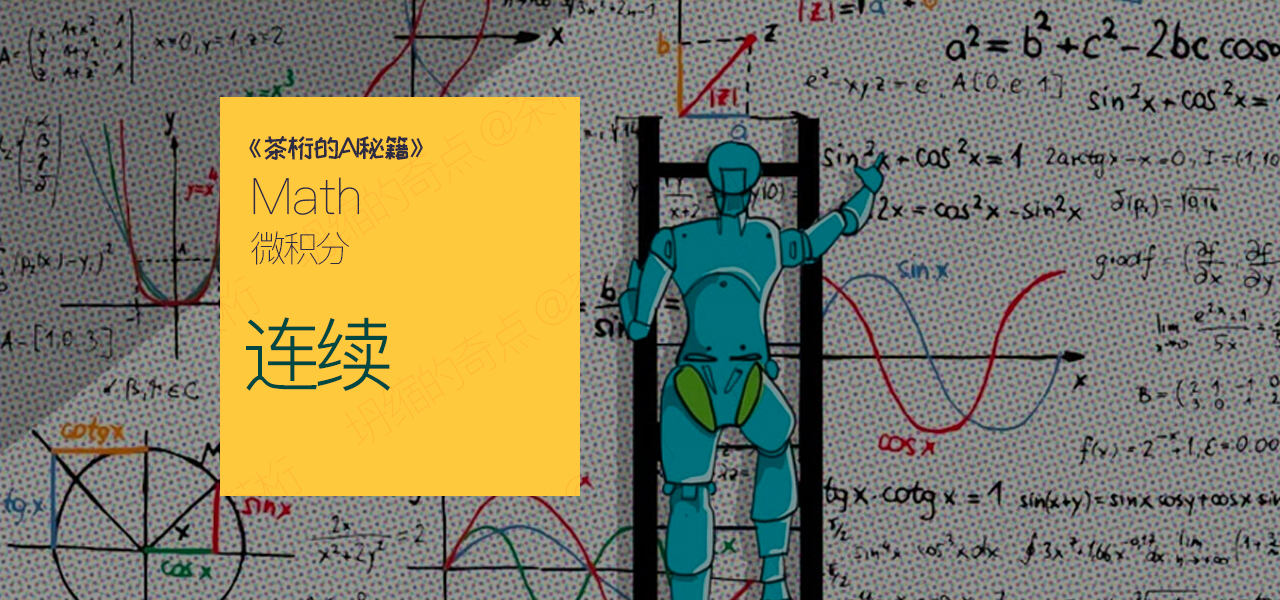
\includegraphics[width=1\textwidth]{asset/茶桁的AI秘籍_Math_8.png}
\end{figure}

\newpage

上一节课我们讲了极限, 很多小伙伴下来后跟我留言说有点懵. 不必太过在意, 慢慢的多看几遍去理解, 并且, 极限也并不是特别核心的问题, 暂时先放一放也可以. 

本节课, 我们要讲的内容是「连续」. 

\section{连续}

首先我们从直观上想一下, 在日常生活里面这个连续它给我们一些什么样的印象?可能会优先想到这么几点: 

\begin{itemize}
  \item 一个是不断裂. 
  \item 其次是不跳跃
  \item 处处相连
\end{itemize}

那咱们先来看第一点不断裂. 打比方说, 本来有这么一个函数图像好好的, 但是我们在它中间断了一个点, 就这么一个点就是一个老鼠屎坏了一锅粥. 连续就应该是不断裂的, 不能象图\ref{fig:img9_1}一样.

第二点是不跳跃. 如函数图\ref{fig:img9_2}, 这个函数本来在前面一段$x_0$这一点的函数值还在下面, 结果下一步就一下跃升到上面去了, 它有个跳跃. 这和我们日常生活中理解的连续也是不一样的. 

\begin{figure}[ht]
  \centering
  \begin{minipage}[h]{0.4\textwidth}
    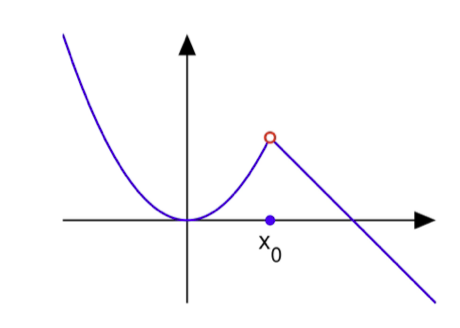
\includegraphics[width=\textwidth]{asset/aa29dda5-78fc-480a-b2ac-f1692445d496.png}
    \caption{断裂}
    \label{fig:img9_1}
  \end{minipage}%
  \hspace{2em}
  \begin{minipage}[h]{0.3\textwidth}
    \includegraphics[width=\textwidth]{asset/63c70c64-4dda-41c6-94b5-9f88083516d0.png}
    \caption{跳跃}
    \label{fig:img9_2}
  \end{minipage}
\end{figure}

还有第三个: 处处相连. 其实只要不是上面这两种情况, 那基本上就是处处相连的. 如图\ref{fig:img9_3}, 就像我们当前这个图像所描述的一样, 任何一个地方都是连接在一起的, 就像一条锁链一样都是连接在一起的. 它并没有像上面两个函数图像一样出现断裂或者跳跃, 这个就是直观上面的. 

\begin{figure}[ht]
  \centering
  \includegraphics[width=0.3\textwidth]{asset/a5406854-3b3e-427c-b296-e56f004f1568.png}
  \caption{处处相连}
  \label{fig:img9_3}
\end{figure}

\paragraph{连续的正式定义如下}:

\begin{newquotation}
  设函数$f(x)$在点$x_0$的某个邻域内(例如:$(x_0 - 0.0001, x_0 + 0.0001)$)有定义, 如果有: \(\lim_{x \to x_0}f(x)=f(x_0)\), 则称函数f(x)在点$x_0$处连续, $x_0$称为函数$f(x)$的连续点. 
\end{newquotation}

定义中说: 函数$f(x)$在点$x_0$的某个邻域内, 邻域是什么意思呢?我们拿定义里的例如来说, $x_0$向左走了$0.0001$个单位, 然后$x_0$还向右走了$0.0001$个单位, 这个新的区间, 就称为$x_0$的邻域. 当然, 这个邻域的范围可以再小一点, 我们可以在这个单位前面再添加几个0. 如果函数$f(x)$在点$x_0$的某个邻域内有定义, 有定义就是这个蜡烛的光能照到这个手, 就叫做有定义. 要看懂我这个比喻需要前面的课上过是吧?也有可能有小伙伴没上过呢. 那好吧, 重新来说, 有定义就是可以映射. 

我们接着继续看, 如果有$\lim_{x \to x_0}f(x)=f(x_0)$这个式子, 那意思就是$f(x)$它在$x$趋近于$x_0$的时候, 极限的取值等于$f(x_0)$这个函数它在这一点的函数值, 我们就称它在点$x_0$处连续. 

稍微的来理解一下这个定义, 来看图\ref{fig:img9_4}: 

\begin{figure}[ht]
  \centering
  \includegraphics[width=0.4\textwidth]{asset/00036f9b-aad5-4c4e-b1a2-c7a287d93f1d.png}
  \caption{}
  \label{fig:img9_4}
\end{figure}

在$x_0$上方红圈$a$那一点的极限, 按照之前学的极限的概念来看, 在这里取值应该是对应的是趋近于a的值, 那么应该是趋近于$y_0$这么一个Y值, 但是函数在$x_0$的取值是等于0的, 也就是图中函数的$a$点值, 我们给它挖出来落在了X轴上, 这一点落在了X轴上面Y值就等于0. 所以函数在$a$这一点的函数值和它在这一节的极限不相等, 就出现了断裂. 

所以如果极限$\lim_{x \to x_0}f(x)$和$f(x_0)$这个函数值相等, 我们就说它在点$x_0$处是连续的, $x_0$也可以被称为函数$f(x)$的一个连续点. 

好吧, 我知道这个时候一定有些人又开始懵了. 如果学一个东西的时候, 能自己主动的去查去找解决办法是非常赞的. 但是也要给自己设立一个止损的时间. 有一个点如果自己一直想不通, 可能得换一种方法去解决他了. 比如说问一下其他人, 寻找一些其他可以引导你的方法. 网上很多课程所讲的角度和细节都不太一样, 有很多时候, 两篇文章的细节凑在一起的时候, 就忽然的开窍了. 或者也许, 以后我会忽然觉得那么讲好理解一点, 就再用其他方法讲一遍,忽然之间你就开窍了呢。

不管如何, 都要给自己设定一个止损时间, 如果你不给自己设一个时间, 会极大的损害学习的动力. 一开始的学习热情, 被一些一直攻不破的东西给消耗了, 这是一件得不偿失的事情. 

我们回过头来总结一下前面的内容, 可以说, 函数在连续点的极限就是连续点的函数值. 大家其实只要记住上面那一个图就行了. 明明在那一点上是连续的, 可是非要人为把a点的值挖出来放在x轴上, 也就是$x_0$这一点, 那肯定就变成不连续的了. 

接着, 我们来看一个证明: 

\begin{align*}
  \mbox{例子: } & \mbox{证明函数} f(x) = x^2, x \in R, \mbox{在 x=0处连续. } \\
  \mbox{解}: & \mbox{由题干易知}, f(0) = 0^2 = 0, \mbox{接下来验证}x = 0\mbox{处函数的极限值是否是}0: \\
  & \mbox{对任意} \varepsilon > 0, \mbox{取} \delta = \sqrt {\varepsilon},  \\
  & \mbox{则: } 0 < |x-0| < \delta , \\
  & \mbox{有: } |f(x) - 0 | = | x^2 - 0| < \delta ^2 = \varepsilon \\
  & \mbox{所以} f(x)\mbox{在 x= 0 处的极限为0} \\
  & \mbox{所以} f(x)\mbox{在x=0处连续}
\end{align*}

其实, 这个函数式, 我们在图上画一个函数图像就很清楚的看到结果. 不过肉眼看到的并不是百分百精确.

数学和物理有一点是不一样的. 物理提出一个假设, 然后去验证, 在已知范围内没有一个实验的结果是推翻他的, 或者说反驳他的, 那就可以承认这个理论是存在的. 但是数学不行, 只要没有证明全部的情况都是合理的, 都是符合这个假设的话, 都不能说它是一个真正的一个定理. 

所以, 数学和物理在这方面差别很大. 当然, 物理学虽然承认的一些定理其实也是有阶段性的. 像牛顿的万有引力定律, 或者说宏观物体的运动规律, 牛顿三定律在宏观、低速状态下其实是OK的. 但在微观或者说超高速的情况下其实又不存在了. 

所以物理理论自己也知道, 大概在哪些范围之内是存在的, 随时准备接受以后的这些实验来推翻或者说改进它. 

我们来看一下刚才这个证明的例子. 

首先判断一个函数是不是连续的怎么判断?我们看它的在这一点的函数值是什么, 在这一点函数值是$f(0) = 0$, 这个就没什么可说的. 接下来我们唯一需要做的就是$x=0$的时候函数的极限是否是0, 会不会跳到其他地方去, 就像图\ref{fig:img9_4}里面一样. 

在这里因为要考虑极限, 所以还是用上一节所说的极限的知识去做, 对于任意$\varepsilon > 0$,  然后取$\delta$等于$\sqrt{\varepsilon}$, 因为$\varepsilon$别人塞给你的你没法改, $\delta$可以自己随心所欲. 只要能证明出来下面那些就OK, 所以$\delta$其实是我们设计出来的. 然后$x-0$, 0这一点实际上就是$x_0$点, 它在这个范围之内的时候就有$f(x)$减去我们假设的这个极限, 然后就等于$|x^2 - 0|$, 也就是$x^2$的绝对值. 

当然了, $x^2$本身就是一个非负数, 绝对值也可以拿掉. 所以其实就是$x^2$. $x^2$根据式子是小于$\delta^2$的, 根据式子$\delta^2 = \varepsilon$,  那我们就恰好证明出来了, 函数值减去假设的极限, 确实小于任意的$\varepsilon$. 

这里的任意体现在什么地方?大家可以这样想,$\varepsilon$这里可以取0.01, 那这个时候$\delta$等于0.1, 这样带入进去一路算下来没有问题, $\varepsilon$再继续小, 比如说$10^{-10}$, 按照规则, 式子依然成立. 这个才是极限的魔力所在, 也是「任意」体现的地方. 

「任意」, 没什么数学基础的同学可能会想到什么?你刚才说的都是$\varepsilon$任意小, 那为啥不提这个$\varepsilon$特别大的情况? 其实, 特别大的情况没必要去考虑, 比如我告诉你一个数, 然后我让你猜大小, 你猜5, 我跟你说这个数比5还小, 那你会不会还往比5大的方向去猜?你会不会跟我说这数是不是10?不可能对吧?

所以虽然它是任意, 但其实我们去做这样的证明的时候, 关注的方向是他非常小的那么一刻. 因为只要非常小的时候都能满足这个式子, 那非常大的时候肯定是满足的. 所以虽然写的是「任意」这两个字, 但是大家要注意其实它真正关心的是$\varepsilon$非常小的情况. 

那我们就证明出来, $f(x)$在$x_0$处的极限就是0. 既然这个函数在这个点的极限是0, 函数值又是0, 那根据我们上面的结论, 这个函数就是在$x=0$处就连续了. 

OK, 极限、连续这两个比较痛苦的过程暂告一段落了. 因为大家以后如果去做AI算法工程师或者去做其他一些算法方面东西、AI模型方面的东西, 仍然有可能会涉及到这些数学方面的概念. 所以在这里大家也要有一个了解, 至少你要直观上面知道他描述了什么样的一个东西. 

如果不是如此, 大家甚至都可以选择略过这两节课. 当前我讲课主要是为了保证学科上的一个连续性. 

% \chapter{微积分: 导数}

\begin{figure}[ht]
  \centering
  \includegraphics[width=1\textwidth]{asset/茶桁的AI秘籍_Math_9.png}
\end{figure}

\newpage

我们终于结束了极限和连续的折磨, 开启了新的篇章. 

不过不要以为后面的就会很容易, 只是相对来说没有那么绕而已. 

那么, 我们今天开始学习「导数」. 

\section{导数}

在之前的导论, 也就是基础课里我们已经接触了导数. 在里面曾经提到, 「导数」和人工智能是最相关的一个概念. 我们再来回顾一下它的相关概念, 看看它的正式的定义是怎样的: 

\begin{align*}
  y' = \frac{dy}{dx} = f'(x) = \lim_{h \to 0} \frac{f(x+h) - f(x)}{(x+h) - x}
\end{align*}

来看这个定义, 一共三个等号. 其中$y'$、$\frac{dy}{dx}$、还有$f'(x)$, 都是导数的一种表示方式. 最后一个等号右边, 就是导数的正式定义, 当h趋近于0的时候, 在这个函数图像上分别取了两个点, 一个是$x$, 一个是$x+h$. 这两个点的距离不断缩小, 也就是当这个h不断趋近于0的时候, 函数图像上的这两点就几乎重合了. 

\begin{figure}[ht]
  \centering
  \includegraphics[width=0.5\textwidth]{asset/d46aa419-f50b-4bfd-83eb-d807f3c821a0.png}
  \caption{}
  \label{fig:img10_1}
\end{figure}

在之前的课程中我们也提到过. 这两点无限接近, 几乎重合的时候, 两点就归于一点了, 在上方图像中, 也就是$P_0$这一点. 这个点在函数图像上面就代表了一个切线, 也就是形成角$\alpha$的红色这条线. 所以, 导数的几何意义其实就是代表了这个函数图像上面一点的切线斜率, 并且代表了函数图像上这一点变化的快慢情况, 也就是这一点的变化率. 

任意函数的导数都可以通过这个定义式求解, 不过就是有的简单, 有的比较繁琐的而已. 前提是这个函数可导, 就是可求导. 它的这个导数可以按照我们定义的这个式子去做. 那问题来了, 有不可导的函数吗?

有, 而且还非常多. 说一个非常常见的,比如

\begin{align*}
  y=|x|, x \in R
\end{align*}

这个函数的函数图像如图:\ref{fig:img10_2}: 

\begin{figure}[ht]
  \centering
  \includegraphics[width=0.5\textwidth]{asset/22572127-4cbd-4f9d-88bc-7ded3cd6940f.png}
  \caption{}
  \label{fig:img10_2}
\end{figure}

我们看这个函数, 首先, $x\in R$, R代表的是实数集, $\in$表示的是属于, 也就是符号左边属于右边的集合, 它表示这种属于的关系. 

$y=|x|$可以写成分段函数的形式, 也就是下面这种形式: 

\begin{align*}
  y = f(x) =
  \begin{cases}
  -x, x<0 \\
  x, x \geq 0 \\
  \end{cases}
\end{align*}

当$x \geq 0$的时候,就是$x$本身, $x<0$的时候那就要添加一个负号, 负负得正. 

所以当我们单独的看这两个分段的时候, 我们会发现从0的左侧求导数的话, 结果是-1. 

因为我们说过导数的几何意义就是函数图像的切线斜率. 因为这条线就是一条直线, 那这上面的每一点的切线都和这条线本身重合. 所以这条线的斜率它就是-1. 

右边这一节的斜率就等于1, 在这种情况下的话, 它的左导数等于-1, 他的右导数等于1, 这两个不相等. 在同一个点0这里出现了矛盾. 左边说: 你得等于-1, 可是右边又说: 不行, 你得等于1. 

所以在这种情况下它的导数本身在这点就产生了矛盾, 所以它的导数是不存在的, 我们把后面的推导补全, 就是: 

\begin{align*}
  & f'(x) = \begin{cases} -1, x<0 \\ 1, x \geq 0 \end{cases} \\
  & \mbox{从0的左侧求导数: } f'(0-) = -1, \\ 
  & \mbox{从0的有侧求导数: } f'(0+) = 1 \\ \\
  & f'(0-) \neq f'(0+)
\end{align*}

这个例子还是非常简单的, 大家应该都学过$y=|x|$的函数图像. 但就这么一个例子就能告诉我们导数不存在可以是长成什么样子的. 那从这个导数的例子里我们还可以得到一个什么结论?就是\textit{函数可导一定是连续的, 但是连续的不一定是可导的}. 

当然我们上一节导论课也已经说过很多关于导数的东西, 比如怎么样用定义去求一个东西的导数, 在导论课里面我们已经求了为什么正弦函数$sinx$导数是$cosx$, 大家如果忘记的话可以再回去看一下之前的课程\hyperlink{6.微积分-函数}{《6. 微积分 - 函数》}. 

\section{求导实例}

接下来, 我们看一下这个例子: 

\begin{figure}[ht]
  \centering
  \Large{例: 求函数 $y=x^x$ 的导数}
\end{figure}

现在我们要求导数, 怎么去求?在导论课里面我们上过哪些概念?我们当时有一个表列出了「常用函数的导数」对不对, 小伙伴们还记不记得?不记得也没关系, 我们这里再列一下.

\begin{table}
  \centering
  \begin{tabular}{ll}
    \midrule
      $C' = 0$ & $(x^n)' = nx^{n-1}$ \\
      $(sinx)' = cosx$ & $(cosx)' = -sinx$ \\
      $(a^x)' = a^x \ln a$ & $(e^x)' = e^x$ \\
      $(log_a{x})' = \frac{1}{x}log_a{e}$ &  $(\ln x)' = \frac{1}{x}$ \\
    \bottomrule
  \end{tabular}
  \caption{常用函数的导数}
  \label{fig:table10_1}
\end{table}

表\ref{fig:table10_1}中就是常用函数的导数, 似乎这里面没有我们可用的, 也就是通过常用函数的导数没法解. 

接下来, 我们再想想之前的课程还学过什么?之前还学过导数的一些运算法则, 来回忆一下: 

\paragraph{导数的运算法则}:

\begin{align*}
	\begin{split}
    & \mbox{设} u = u(x), v = v(x)\mbox{可导, 则: }\\ \\
    & (1) (u\pm v)' = u'\pm v' ; \\
    & (2) (cu)' = cu' (C\mbox{是常数}); \\
    & (3) (uv)' = u'v+uv'; \\
    & (4)(\frac{u}{v})' = \frac{u'v-uv'}{v^2}(v \ne 0)
	\end{split}
\end{align*}

可是在这种情况下似乎还是没有什么思路, 就是说$x^x$似乎并不是这四种组合里的其中一个, 所以这该怎么办?

这得费点脑子了, 让我们来一步一步看. 

首先, 两边同取对数. 对数运算大家应该都知道吧?比如说$3^2$, 这个结果等于多少?等于9对吧?

我们都知道$x^2$是一种乘方运算, 是针对指数的运算. 告诉你3的几次方, 都能算出来, 因为你知道3的平方等于两个3乘在一起, 3的3次方等于3个3乘在一起. 

那我问你, 3的x次方等于9你咋做?对数运算, 也就是刚才说的乘方运算反过来. 一个正一个反, 乘方运算是告诉你3的平方让你求结果. 对数运算就是3的多少次次方等于9, 然后求它指数, 也就是它是几次方. 这就是对数的意思. 

如果小伙伴们还不太清楚, 可以自行Google一下. 这个太基础了, 就不多讲了. 我们接着来看当前这道题, 求$y=x^x$的导数. 

首先, 两边同取对数, 为什么两边同取一个对数?因为不管是什么样的运算, 只要等式两边是相等的, 不管做什么运算, 两边做同样的一个运算相等的结果仍然不会变.

\begin{align*}
  \ln y = x ln x
\end{align*}

$\ln y = x \cdot \ln x$, 其实是$\ln x^x$变化过来的. 对数运算有个特点, 就是x上面的指数部分可以拿在前面和它乘在一起. 所以这里是$x \cdot \ln x$.

接下来, 两边同时对x求导, 在这里关于导数的运算法则就可以用上了, 相当于是导数的嵌套.

因为y是关于x的函数, 所以两边先都关于x进行求导:

\begin{align*}
  \frac{d}{dx}(lny) = \frac{d}{dx}(xlnx) 
\end{align*}

左边咱们用链式法则来处理, 链式法则下节会讲, 这节课先知道这么用:

\begin{align*}
  \frac{d}{dx}(lny) = \frac{1}{y} \cdot \frac{dy}{dx} 
\end{align*}

这里的$\frac{dy}{dx}$就表示$y$对$x$的导数, 也就是$y'$, 所以就变成$\frac{1}{y} \cdot y'$, 也就是$\frac{y'}{y}$. 这是左边, 我们再来看右边. 

右边就是我们刚才那个导数运算法则里面的这个函数式$(uv)' = u'v+uv'$, 就是两个函数乘在一起求导, 分别等于其中一个求导再乘以另外一个, 之后将两者相加. 

我们来看, 先对x求导, x求导就变成1, $\ln x$不变拿过来, 就是$1 \cdot \ln x$, 然后再加上$\ln x$求导, 求导结果是$\frac{1}{x}$,  这次x不变拿过来. 我们就得到了这样一个式子: $1 \cdot \ln x + x \cdot \frac{1}{x}$. 再化简之后, 就得到了: $\ln x + 1$. 

最后我们就得到$\frac{y'}{y} = \ln x + 1$. 

继续, $y'$应该等于$y \cdot (\ln x + 1)$, 我们再把y用$x^x$代换一下, 最终我们得到$x^x(\ln x + 1)$. 

那我们最终是要求什么?是不是就是求$y'$, 那现在我们最终就得到了$y' = x^x(\ln x + 1)$为我们所求.

然后我要求大家去做的事就是大家可以自己去查一下对数、对数函数是怎么一回事, 以及它为什么有这样的性质: $ln x ^x$为什么就等于$x \ln x$. 也就是, 我们为什么可以将指数拿到前面去, 和对数函数相乘. 这部分应该是高中的内容. 

最后完整的推导过程就是: 

\begin{align*}
  & \frac{y'}{y} = 1 \cdot \ln x + x \cdot \frac{1}{x} \Rightarrow \frac{y'}{y} = \ln x + 1 \\ \\
  & \mbox{所以} y' = y(\ln x + 1) = x^x(\ln x + 1)
\end{align*}

接下来, 我们做一个比较有意思的事情, 我们做一个代码的演示. 上数学课这么久, 好久没接触代码了是不是?连我都有些小激动. 我们用代码来演示一下, 迭代法求解二次函数最小值, 来让我们开始: 

\section{代码演示: 迭代法求解二次函数最小值}

首先, 还是一样, 大家应该还记得如何导入需要的方法: 

\begin{python}
import numpy as np
import matplotlib.pyplot as plt
from IPython import display
\end{python}

在之前的Python课程中已经详细的讲解过Python的相关知识, 所以这里就不一一进行解释了. 

让我们先定义一个二次函数: 

\begin{python}
def f(x):
    y = x**2
    return y
\end{python}

紧接着, 我们还需要定义一个对应的导数: 

\begin{python}
# 定义对应的导数
def d(x):
    dy = 2*x
    return dy
\end{python}

这一步应该都看得懂吧?$y=x^2$对应的导数$y'$就应该等于$2x$. 

现在我们定义了两个自定义函数, 接下来希望将程序做成一个交互性的, 所以我们需要一个操作者输入指定的x初始值的操作: 

\begin{python}
# 操作者输入指定的x初始值
x = float(input('请输入x的初始值: '))
\end{python}

之后, 这段代码会给出一个动画的演示过程出来, 大家可以看得比较清楚我们是怎样在人工智能里面通过这种不断的迭代去求解一些神经网络的一个最优化的解. 

这里我们举一个比较简单的例子: 二次函数的最小值的求解过程. 

下面我们需要定义一个学习率, 并且准备一段二次函数数据点: 

\begin{python}
# 定义学习率
lr = 0.9

# 准备一段二次函数数据点
x_temp = np.linspace(-x, x, 1000)
y_temp = x_temp**2
\end{python}

\textbf{之后整个一段`while`循环, 都是为了输出图像的}, 之前我们学过`matplotlib`对吧, 这里就不详细的进行代码解释了, 大家下来可以执行研究一下代码, 我们主要是为了进行动画演示, 大家其实这里也不需要太了解, 不是主要目的: 

\begin{python}
while abs(x) > 0.01:
    # 用于清空之前的输出
    display.clear_output(wait = True) 
    # 清除之前的列表
    plt.clf()
    plt.plot(x_temp, y_temp)
    plt.scatter(x, f(x), s=30, c='red')
    plt.show()
    print('此时x的值为: ', x)
    plt.pause(0.7)
    \%matplotlib inline
    dy = d(x)
    x -= lr * dy
else:
    display.clear_output(wait=True)
    plt.clf()
    plt.plot(x_temp, y_temp)
    plt.scatter(x, f(x), s=30, c='red')
    plt.show()
    print('最终x的值为: ', x)
\end{python}


对于y等于x平方的二次函数. 我们要看它什么?先给它设一个起点, 比如说点5吧, 然后看它怎么样一步一步的逼近最小值点. 现在我们来看一下图\ref{fig:img10_3}: 

\begin{figure}[ht]
  \centering
  \includegraphics[width=0.5\textwidth]{asset/截屏2023-12-31 12.45.38.png}
  \caption{动图无法正常显示, 点击\href{https://raw.githubusercontent.com/hivandu/notes/main/img/20230830160512.gif}{查看原图}}
  \label{fig:img10_3}
\end{figure}

从一开始的点, 一点一点迭代, 是不是越来越靠近最小支点了?就是这样一步一步的迭代, 直到达到我们要求的误差范围之内. 就是说我们给定了一个最小误差在多少以内, 当到达之后, 它就停止了. 我们设定的值是$0.01$, 所以它最终$x$的取值是 $0.009671406556917058$. 

这个就是整个过程, 大家不要看着似乎很简单, 其实人工智能, 或者严格意义上来说是神经网络怎么优化?就是这么优化. 随机初始化一些参数, 然后这些参数就从刚才我们类似于$x=5$的点一步一步通过迭代不断的逼近最优解. 不断的逼近直到达到一个范围之内, 而且在这里我们是可以定义学习率的. 大家应该看到我代码里设置了一个学习率`lr = 0.9`. 学习率就是我每一步走多远, 你比如说在这里是0.9, 如果我们弄成0.2的话大家看一下会发生什么, \ref{fig:img10_4}: 

\begin{figure}[ht]
  \centering
  \includegraphics[width=0.4\textwidth]{asset/截屏2023-12-31 12.50.40.png}
  \caption{动图无法正常显示, 点击\href{https://raw.githubusercontent.com/hivandu/notes/main/img/20230830160512.gif}{查看原图}}
  \label{fig:img10_4}
\end{figure}

整个过程中, 每一步走的比较慢. 所以他就不会像刚才一样每一步跨的比较大, 两边对称轴一直在反复晃, 现在的消息就是单侧逼近了. 所以, 其实不管你再怎么复杂的神经网络, 都是用求导反向传播, 然后通过乘上优化算法、设置学习率去做的. 不管多么复杂的原理其实都是这么简单. 

大家肯定会觉得很神奇, 有没有人会认为我在蒙你们?神经网络那么复杂的东西, 那么复杂的任务都可以胜任, 原理居然这么简单. 对, 就是这么简单, 只不过它复杂在哪?它的网络结构可以很多样化, 第二个是它的优化方法可以很复杂, 以及他是不是添加到一些其他的量. 这些都是需要我们去考虑去设计的, 但是最根本的核心就是上图演示的这么一个过程. 

所以大家不要觉得AI和我们离得非常远, 就是显得好像我们和AI触手不可及一样, 原理其实都很简单. 

就比如二八定律是一个非常朴实的一个定律, 不管是在经济学领域还是在其他领域, 我个人觉得都是很适用的. 就像神经网络, 如果你说原理的话, 我们花20\%的时间可能就可以学到他80\%的东西了, 但是如果我们要学比较深入的一些内容, 往深度去学的话, 为了剩下那么20\%的内容可能我们得填上80\%的时间. 

展示就先到这一步, 在神经网络里面去优化整个网络的这么一个过程. 

\section{阶}

这里再提一个概念, 就是大家可能会看到经常有个术语叫什么几阶导数, 其实阶是什么意思呢?几阶就是对函数求几次导. 比如我们看下面这个函数, 就是二阶导数: 

\begin{align*}
  f''(x) = (f'(x))'
\end{align*}

这里我们对其求了两次导, 所以「阶」的含义就是: 几阶就对函数求几次导. 

再比如我们看下面例子: 

\begin{align*}
  \mbox{例子: 已知函数} \quad f(x) = 3x^4 + 5x^3 + 6x + sinx, \mbox{求其一阶及二阶导数}
\end{align*}

一阶导数, 就直接对先求一次导, 按照我们的求导法则, 这里就不赘述了, 大家可以自己尝试下自己查表去算. 结果我放在下面: 

\begin{align*}
  \mbox{一阶导数: }f'(x) = 12x^3 + 15x^2 + 6 + cosx
\end{align*}

二阶导数什么意思呢?就又对一阶导数再求一次导, 把一阶导数看作是一个原函数, 然后再对他去进行一个求导. 

比如说$12x^3$, 3拿下来和12乘在一起, 计算结果就是$36x^2$, 那之后的每一步也就非常清晰该怎么做了对吧?那结果就是: 

\begin{align*}
  \mbox{二阶导数: } f''(x) = 36x^2 + 30x - sinx
\end{align*}

理解原理之后, 拿常用函数的导数和求导公式过来套就可以了. 大家以后要多做练习. 

% \chapter{微分\&链式法则}

\begin{figure}[ht]
  \centering
  \includegraphics[width=1\linewidth]{asset/茶桁的AI秘籍_Math_10.png}
\end{figure}

\newpage

我们上节课讲了导数. 今天将会是两部分, 一部分是「微分」, 一部分是「链式法则」. 

\section{微分}

微分, 我们在导论里面提过. 它和导数比较像, 但是还是有差别的. 实际的定义和内容都比较简单, 我们先来看看定义:

\begin{align*}
  & \mbox{当自变量x的变化趋于无穷小时}(dx), \mbox{因变量}f(x)\mbox{的变化情况}(df(x)) \\
  & df(x) = f'(x)dx
\end{align*}

当自变量$x$的变化趋于无穷小的时候,我们用$dx$来表示. 因变量$f(x)$的变化情况, 我们用$df(x)$来表示, 在这里$df(x)$等于$f'(x)dx$. 

所以微分它和导数是不一样的. 导数是什么?是函数在某一点的\textbf{变化率}, 是$\frac{df(x)}{dx}$. 微分呢, 是函数在某一点的\textbf{变化量}, 所以一个是\textbf{变化率}一个是\textbf{变化量}. 这就是它们唯一的区别. 

那他们之间有什么联系?我们说: 函数的变化量与自变量变化量之比, 即为导数. 

\begin{align*}
  \frac{df(x)}{dx} = f'(x)
\end{align*}

这些都是从式子得来的, 没什么复杂的地方, 那微分就是这样, 没有更多的内容了. 

接下来, 我们要来学习一个比较重要的概念, 就是链式法则. 

\section{链式法则}

「链式法则」为什么重要. 我们知道神经网络不是只有一层或者两层, 它是有很多层. 比如, 何凯明等人在2015年提出的ResNet, 那个网络就有152层. 后来据说这些网络可以上到1,000层, 太可怕了. 

我们通过上一节课的动图演示, 知道了是怎么样优化的. 就是通过求导, 然后一步一步的去逼近最小值点去做的. 那问题就来了, 求导只是一层的关系, 后面几层的这些导数怎么传到前面几层?这里就对应着嵌套函数的问题. 

什么叫嵌套函数?就是函数里面套上函数. 

打个比方: $y=f(x)$, $x=g(z)$, $x$又是关于$z$的一个函数. 所以, 我们把它写成一个复合函数的形式, 或者说把$y$用z当作自变量来表示:

\begin{align*}
  \mbox{嵌套函数:}& \\
  & y = f(x), x = g(z) \quad \Rightarrow \quad y = f(g(z))
\end{align*}

就是说$f$里面再套一层$g$,然后是$z$. 

好, 我们这个时候来思考一下, 它里面隔着两层函数, 我们怎么样求$y$相对于$z$的一个导数呢? 在这里就需要通过链式法则. 链式法则是怎么得来的?这里一步一步的给大家讲, 先看完整推导式:

\begin{align*}
  y'_z & = \frac{dy}{dz} = \frac{dy}{dz} \cdot 1 = \frac{dy}{dz} \cdot \frac{dx}{dx} = \frac{dy}{dx} \cdot \frac{dx}{dz} \\ \\
  & = f'(x)g'(z) = f'(g(z))g'(z)
\end{align*}

首先,按照导数定义 $y$ 相对于 $z$ 的导数,那就是 $\frac{dy}{dz}$.

然后我们乘以一个1, 它还是不变. 接下来把1可以转化为 $\frac{dx}{dx}$. 

之后将分母调换一下, 把$dx$换过来, 然后把$dz$拿到另外一边去. 通过这么一步变换, 我们就得到 $\frac{dy}{dx} \cdot \frac{dx}{dz}$. 

这一步之后, 现在我们可以套导数定义, 我们惊奇的发现, $\frac{dy}{dx}$不就是$f'(x)$, 而$\frac{dx}{dz}$也正好就是$g'(z)$. 这一步, 是因为$x=g(z)$, 所以$\frac{dx}{dz}$就是函数$g(z)$的导数. 

所以最后, 我们就得到了$f'(x)g'(z)$, 原来$y$隔着一层相对于$g(z)$的导数可以写成$f'(x)g'(z)$的形式. 那我们已知$x=g(z)$,  那我们最后就可以得到$f'(g(z))g'(z)$, 它是中间隔着一层的这么一个关系. 

就是嵌套函数求导的一个方法. 而且不管你有多少层, 你套100万层, 只要它是可导的你都可以这样去做. 方法概括一下, 就是先外层求导, 然后再内层求导. 

我们再来看一个例子:

\begin{align*}
  \mbox{例}:& y = x^2, x=e^z, \mbox{求y相对于于z的导数} \\
\end{align*}

让我们求函数$y=x^2$, $x=e^z$, 然后求$y$相对于$z$的导数. 

$y$关于$z$的导数怎么求? 我们来看:

\begin{align*}
  y'_z & = \frac{dy}{dx} \cdot \frac{dx}{dz} = (x^2)'(e^z)' \\
  & = 2x \cdot e^z = 2e^z \cdot e^z = 2e^{2z}
\end{align*}


套用刚才得到的那个结论, $y'_z$ 就等于$\frac{dy}{dz}$乘以$\frac{dx}{dz}$, 让我们先做外面一层的导数, 再做里面一层的导数. 

外面一层是$x^2$, 然后里面一层是$e^z$. 求出来之后是$2x\cdot e^z$. 

因为我们是求$y$关于$z$的导数,所以我们结果里面不应该出现$x$. 所以我们再把$x$换成用$z$表示的形式. 那很多人就觉得做到这一步就可以了, 但是我们在这里需要把$x$也用z来表示一下, 最终结果应该是$2e^2z$. 

如果嵌套n多层呢, 如果是非常复杂非常复杂, 一直到$x_n = f_{n-1}(x_{n-1})$, 在这么一个映射法则之下会怎么样呢? 

\begin{align*}
  \mbox{如果嵌套N多层...} & \\
  & x_2 = f_1(x_1), x_3 = f_2(x_2), ..., x_n = f_{n-1}(x_{n-1}) \\ \\
  & \frac{dx_n}{dx_1} = \frac{dx_n}{dx_{n-1}} \cdot \frac{dx_{n-1}}{dx_{n-1}} \cdot ... \cdot \frac{dx_2}{dx_1}
\end{align*}

如果是这样, 那也仍然是一样的, 就是逐层求导. 

大家在课后或者复习的时候再看一看链式法则. 它是非常精妙的一个东西, 虽然简单, 但是神经网络的反向传播、后面的这些误差怎么样传播到前面的这些层就靠链式法则, 没有它就不行. 

而且, 链式法则看上去很简单, 但是它的真面目就是我一再强调的\textbf{神经网络的优化原理}、\textbf{反向传播的基石}. 我们看图\ref{fig:img11_1}:

\begin{figure}[ht]
  \centering
  \includegraphics[width=0.8\linewidth]{asset/20200603174921-1878265324_jpeg_759_542_46786.jpg}
  \caption{}
  \label{fig:img11_1}
\end{figure}

这张图上有很多让人头晕的符号, 我们不用去管, 就知道是怎么回事就行. 

就是上面这些层的误差是不断的求导, 通过链式法则传播到前面. 每一层与每一层之间就相当于嵌套了一层函数, 就像我们刚才说的嵌套函数一样. 

本节课我们稍微提了一下「微分」, 然后着重讲了一下「链式法则」,下节课我们讲一下「偏导数」、「方向导数」. 
% \chapter{微积分 - 偏导数-方向导数}

\begin{figure}[ht]
  \centering
  \includegraphics[width=1\textwidth]{asset/茶桁的AI秘籍_Math_11.png}
\end{figure}

\newpage

我们上节课学习了链式法则, 本节课, 我们要学习「偏导数」和「方向导数」. 

\section{偏导数}

偏导数在导论课里面也提到过. 偏导数针对多元函数去讲的. 

多元函数是什么, 我们拿个例子来看: 

\begin{align*}
  \mbox{多元函数: }y = f(x_1, x_2, ..., x_n)
\end{align*}

就是包括$x_1,  x_2,  ...,  x_n$这么多自变量在$f$的映射作用才能得到这么一个$y$. 所以, 它和一元函数的导数的情况不太一样, 它的因变量相对于每一个自变量都有一个导数, 是针对于每一个单独自变量所求出来的导数, 所以称为偏导数. 

偏导数的形式如下: 

\begin{align*}
  \frac{\partial y}{\partial x_1},  \frac{\partial y}{\partial x_2},  ...,  \frac{\partial y}{\partial x_n} \quad \mbox{或者} \quad f_{x_1},  f_{x_2},  ...,  f_{x_n}
\end{align*}

其实和导数一样读作\(dy\),  但是因为需要区别导数和偏导数, 所以就用了\(\partial\), 在Latex中, 写作\pyth{\partial}.

偏导数还可以使用函数本身, 再在右下角加上相对应的自变量来表示. 就比如 $y$ 相对于 $x_1$ 的偏导数, 就可以用$f_{x_1}$来表示. 

不要看它好像很复杂, 这么多的自变量, 我们该怎么样去处理啊?本质上它仅仅是\textit{因为是一个多元函数的导数, 所以才多了一个“偏”字, 而且其求解的过程其实和导数没有任何区别}. 

打个比方说, 求 $y$ 相对于 $x_1$ 的偏导数, 我把$x_2, ..., x_n$ 都看作是常数, 就不用去管它, 只需要关注 $x_1$ 就行了, 其定义的式子也可以显现出这一点: 

\begin{align*}
  \frac{\partial f(x, y)}{\partial x}  = f_x(x, y) = \lim_{h \to 0} \frac{f(x+h, y) - f(x, y)}{(x+h)-x}
\end{align*}

$\frac{\partial f(x, y)}{\partial x}$ 这是一个二元函数,求关于 $x$ 偏导数, 可以写成 $f_x(x, y)$ 这种形式,定义就是说这里虽然是有两个量,但是 $y$ 我不关心, $y$ 就是 $y$ , 我只关心 $x, x+h$, 两者无限逼近的这么一个过程. 

所以,大家可以发现如果把 $y$ 给拿掉,不就是我们求导的过程吗. 

所以偏导数和导数一模一样, 没有任何区别. 

那下面这个例子, 我们在导论课中就已经见到过了,再拿出来也是带大家回顾一下:

\begin{align*}
  \mbox{例: } & \mbox{求多元函数} y = f(x_1, x_2) = x_1^2 + x_1x_2+sinx_2\mbox{的偏导数及导数. }\\ \\
  \mbox{解:  }& \frac{\partial y}{\partial x_1} = 2x_1 + x_2 \\
  & \frac{\partial y}{\partial x_2} = x_1 + cos x_2
\end{align*}

只要导数会求, 偏导数其实就没什么问题. 只要能理解这么个东西怎么求, 就基本上可以和偏导数这一课说goodbye. 

比如我们给出多元函数 $x_1^2 + x_1x_2+sinx_2$ 的偏导数. 那我们怎么求呢?

首先求 $y$ 关于 $x_1$ 的偏导的时候其他的自变量就看做常数, 所以第一项 $x_1^2$ 就求出 $2x_1$, 第二项$x_1x_2$ 就相当于一个常数乘上$x_1$, 常数就是$x_2$. 

然后第二个式子,是 $\frac{\partial y}{\partial x_2}$ 等于什么? 首先我们还是先来看下第一项, 第一项有没有 $x_2$ 呢?没有. 没有的话这一项就相当于一个常数了,对常数求导结果就是0. 为什么对常数求导结果是0我们之前有讲过, 因为常数不管输入是多少, 输出永远是一个恒定的量, 在几何图像上面显示出来就是没有任何变化,就是一条水平线, 所以对常数求导他的导数是0. 

好, 第一项没了. 第二项是$x_1x_2$, 相当于一个常数乘 $x_2$, 常数是$x_1$, 所以这里保留下来. $sinx_2$ 求导就是$cosx_2$. 

多说两句题外话, 偏导数到了实际应用里有什么关联呢?因为我们在人工智能里面, 它不是这种一对一的一元函数关系, 是多元函数关系. 比如说 $sinx, cosx$, 可能不仅产生 $y_1$, 在不同的映射法则之下甚至可能产生 $y_2, y_3$. 所以我们需要了解神经网络里面不是一元函数的导数, 更有可能的是偏导数, 然后逐层反向传播, 这就是偏导数的一个应用. 

\section{方向导数}

我们再来看一下方向导数. 方向导数的内容可能也会稍微复杂一点, 但是因为考虑到课程体系, 有些东西我觉得确实是没办法去删减. 所以在这里也给大家把这部分知识也给讲上. 

我们刚才说的偏导数都是沿着自变量方向的. 比如 $\frac{\partial y}{\partial x}$, 都是沿着自变量方向的, 如图\ref{fig:img12_1}: 

\begin{figure}[ht]
  \centering
  \includegraphics[width=0.5\textwidth]{asset/20230901095029.png}
  \caption{}
  \label{fig:img12_1}
\end{figure}

在这张图里, $x$ 和 $y$ 就是自变量, $z$ 是函数值. 在这种情况下, 偏导数可以沿着什么呢?比如说沿着x的方向把二元函数曲面给截出来, 就如图中这样, 类似一个抛物线的形状. 所以, 偏导数都是沿着自变量的方向. 

那又有一个问题了: 我们能不能沿着任意方向去求导数呢?非得沿着 $x$ 还有沿着 $y$ 去求吗? 确实这是一个好问题. 先说结论, 是可以沿着任意方向求的. 我们来看图 \ref{fig:img12_2}: 

\begin{figure}[ht]
  \centering
  \includegraphics[width=0.5\textwidth]{asset/20230901095643.png}
  \caption{}
  \label{fig:img12_2}
\end{figure}

这张图在绿色这个曲面上面就不一定非得沿着 $x$ 或者 $y$ 方向了. 可以沿着红线的方向, 任意的都可以求. 

又来问题了. 在一元函数里面自变量它在函数曲线上只能沿着两个方向去移动. 我们继续来看图 \ref{fig:img12_3}. 这张图上, 我们在抛物线上X轴左侧随意取一点, 这个点坐落在抛物线上, 要么往上要么往下, 往上就对应着x减小, 往下对应x增大的这么一个方向. 它只能沿着这两个方向,没其他选择了. 

\begin{figure}[ht]
  \centering
  \includegraphics[width=0.5\textwidth]{asset/20230901095921.png}
  \caption{}
  \label{fig:img12_3}
\end{figure}

但是\textbf{在多元函数中,自变量在函数曲面上可以沿着无穷多个方向去移动}. 来继续看一下上面的图\ref{fig:img12_2}: 

就像图\ref{fig:img12_2}里, 在曲面上面任取一个方向, 比如说把红线再稍微转一点它就是一个新的方向,再转一点呢,又是一个新的方向. 

所以在\textbf{多元函数里面,函数的变化不仅和你移动距离有关}, 也就是说不仅和$\partial y$有关, 它\textbf{还和你选择的方向有关}. 

如何得来呢?我们来看: 

\begin{align*}
  \frac{\partial z}{\partial l} \Bigg \vert _p = \lim_{p' \to p} \frac{f(P') - f(P)}{|P'P|}
\end{align*}

对于一个函数 $z=f(x,y)$, 对于函数而言, 我们在这里求它偏导的话就是 $\frac{\partial z}{\partial x}$ 或者 $\frac{\partial z}{\partial y}$, 但是这里我不是比上$\partial x$ 或者$\partial y$了, 而是比上$\partial l$, $l$ 代表着一个方向, 在图\ref{fig:img12_4} 中其实就是红线, 坐落在$x, y$轴线形成的平面上的那一根红线,它代表的一个方向. 

\begin{figure}[ht]
  \centering
  \includegraphics[width=0.8\textwidth]{asset/20230901103919.png}
  \caption{}
  \label{fig:img12_4}
\end{figure}

我们来看一下式子,方向导数的定义式其实和偏导数很类似,只不过它就是沿着l. 我们看到这个图像,它很复杂,是一个二元函数. $x$ 和 $y$ 都是自变量. 跟着我的步骤一步一步, 别自己跑丢了. 

$z$ 是 $x, y$ 的一个函数值. 就像图中绿色字体标出来的一样,$z = f(x, y)$, 所以自变量就可以在 $x, y$ 平面内任意取中一点, 然后在 $f$ 的映射规则下得到一个 $z$ 值, 也就得到竖值方向, 也就是 $z$ 轴上面的一个值, 形成一个曲面. 

当我们现在沿$l$方向去求它方向导数的时候,其实我们还是用无限逼近的原理去做. 

首先, 我们取两个点, 先取点 $P$, 坐标是 $x_0, y_0$, 然后我们取另外一个点 $P'$,$P'$ 对应着曲面上的点是 $Q$ 点, $P$ 点对应的是 $M$ 点. $P$ 和 $P'$ 对应着我们自变量的取值, $M$ 和$Q$ 是我们图像上面的点. 因为 $M$ 和 $Q$ 是有 $z$ 坐标的, 而$P$ 和 $P'$ 是没有的. 

我们就来看一下 $P$ 和 $P'$, 当 $P'$ 不断的向 $P$ 靠近,不断的逼近的时候, 它们中间的长度也趋向于0. 则 $M$ 和 $Q$ 也是趋向于0的. 

在过程当中就采取一个类似类比的思想, 就是我在这里把 $P, P'$ 作$\partial x$, 把这两点的长度看作是 $\partial x$, 也就是我们导数里面的 $\partial x$.  $f(P')$ 其实就是 $Q$ 点在 $z$ 轴上面的值. 再减去 $M$ 点对应的 $z$ 轴上面值, 其实也就是 $f(P)$, 也就是 $f(P') - f(P)$. 

我们定义式, 就可以写成 $\lim_{p' \to P} \frac{f(P') - f(P)}{|P'P|}$ 这个式子. 

大家可以和我们导数的定义式类比一下, 同样一个极限符号, 其中一个点向另外一个点无限逼近, 分母是一个$\partial x$. 在这里的$\partial x$ 就是 $(P,P')$ 的长度,写作 $|P'P|$, 它们函数值之差就是 $f(P') - f(P)$, 也就是区域点的 $z$ 座标值减去 $M$ 点的 $z$ 座标值. 令 $l$ 的方向余弦为: 

\begin{align*}
  (cos \alpha, cos \beta, cos \gamma)
\end{align*}

这里还需要一个概念,叫做 $l$ 的一个「方向余弦」. 方向余弦是什么东西呢?稍后我们就会讲到,先接着之前的继续说: 当我们在这里把 $f(P') - f(P)$ 写出来之后, 它具体的代表其实是下面的这么一行公式: 

\begin{align*}
  \lim_{P \to 0} \frac{f(x_0 + \Delta x, y_0+\Delta y) - f(x_0, y_0)}{P} \\
\end{align*}

$P'$ 相对于 $P$ 点, 它们俩之间的差是怎么得到的呢? 是不是$x_0$ 再加上沿X轴上的一节长度 $\Delta x$, $y_0$ 加上沿Y轴的一段长度 $\Delta y$, 就到达 $P'$ 了. 

也就是说, $P'$ 的坐标就是 $x_0 + \Delta x, y_0+\Delta y$. 因为自变量是两个 $x, y$, 所以函数里面就是 $f(x_0 + \Delta x, y_0+\Delta y) - f(x_0, y_0)$. 

所以, 方向导数 $\frac{\partial z}{\partial l}$, 是曲面在$P$ 点处代表着沿 $\partial l$, 也就是沿着红线方向的变化率. 之前的偏导数要么沿着 $x$ 方向,要么沿着 $y$ 方向. 现在就很自由了, 想沿哪个方向就沿哪个方向, 只要这个方向能求导. 所以, 我沿l方向就被称为沿着 $l$ 方向的方向导数. 也就是半切线$\overline {MN}$ 的一个斜率. 

$\overline {MN}$ 是怎么得到的? 就是 $P'$ 无限逼近 $P$ 的过程当中, $Q$ 也无限逼近 $M$, 就像我们二次函数里面的例子一样,这两个点无限逼近到一块去之后,在 $M$ 点重合,那 $M$ 点这里就有一条切线. 切线的斜率就是方向导数的数值. 也就是它的几何意义. 

大家怎么样去理解呢, 最好是把它和导数那一部分去做一个类比的理解. 分母就是 $\partial x$, 就是自变量的一个差值. 分子部分是函数值的一个差异. 

\subsection{方向余弦}

我们刚才说到有个概念叫「方向余弦」. 方向余弦在接下来的求导过程当中需要用到, 所以我们要了解一下什么是方向余弦. 

余弦大家在初中就接触过, 初中数学就有上过正弦余弦,这里就是在那个基础之上. 它的定义为: 

\begin{newquotation}
  向量与三个(或两个)坐标轴之间的角度的余弦: $cos \theta_1, cos \theta_2, cos \theta_3$
\end{newquotation}

我们来看图\ref{fig:img12_5}: 

\begin{figure}[ht]
  \centering
  \includegraphics[width=0.5\textwidth]{asset/20230901155252.png}
  \caption{}
  \label{fig:img12_5}
\end{figure}

这个向量和这三个坐标轴都会有一个夹角,分别是 $\theta_1, \theta_2, \theta_3$, 如果是平面直角坐标的话, 那它只会和两个坐标轴有角度: $x$ 轴 $y$ 轴, 就没有 $z$ 轴. 如果是三维的情况, 它就三个夹角的余弦值, 组合到一起就叫做「方向余弦」, 分别是$cos \theta_1, cos \theta_2, cos \theta_3$, 这三个余弦的平方和等于1. 

如果是在平面直角坐标系里面, 两个值的情况很好理解. 因为我们只考虑这 $x, y$ 平面, 而不考虑有 $z$ 轴. 那我们现在就只考虑平面: 比如, 这里有一个向量, 它和x轴夹角是30度, 那和y轴夹角就肯定是60度. $cos30^\circ$ 应该是等于 $\frac {\sqrt 3}{2}$, $cos 60^\circ$ 是等于$\frac{1}{2}$, $(\frac{\sqrt 3}{2})^2 + (\frac{1}{2})^2$, 算一下结果就是等于1. 不管是二维还是三维式子, 平方和等于1是始终成立. 

\subsection{投影}

这里又需要多出一个概念叫「投影」, 立体向量 $\vec e$ 在 $x_1$ 方向上的投影就是其自己的本身的长度乘以它和相应的坐标轴之间夹角的余弦值. 如下: 

\begin{itemize}
  \item 向量 $\vec e$ 在 $x_1$ 方向上的投影为: $|\vec e| cos \theta_1$ 
  \item 向量 $\vec e$ 在 $x_2$ 方向上的投影为: $|\vec e| cos \theta_2$ 
  \item 向量 $\vec e$ 在 $x_3$ 方向上的投影为: $|\vec e| cos \theta_3$ 
\end{itemize}

就像一束光打到墙上一样. 本来这个向量箭头非常长, 但是因为有一个角度, 它投射在坐标的某一个方向上, 垂直于某一个方向的时候其实是有一个压缩的, 我们就把它叫做投影. 这和我们生活当中的投影也是非常类似. 所以投影值肯定是比你原来向量长度要小. 

因为三角函数值不可能大于1, 所以肯定不会超过原来向量的长度. 这个其实也是初中数学的内容. 

那我们现在就知道了方向余弦是怎么一回事了. 就是向量和坐标轴之间的一个夹角的余弦组合在一起. 

\subsection{继续讲方向导数}

还是回过去看图\ref{fig:img12_4}, 我们说令l的方向余弦为: ($cos \alpha , cos \beta$), 在图中我们并没有表示出$\alpha$, 其实就是 $l$ 和 $x$ 轴之间的夹角, $\beta$ 就是$l$ 和 $y$ 轴之间的夹角. 

看到这里, 可能有的小伙伴要问了, 三维里面它应该是三个夹角, 那为啥在这里没有说它和 $z$ 轴的夹角?这是因为虽然它图像三维的, 但是自变量只有两个. $z$ 轴其实是它的函数值, 不是自变量, 所以我们就不考虑 $z$ 轴, 只考虑平面, 得到方向余弦只考虑 $x, y$ 这两个坐标轴的一个夹角. 

然后令 $t = |P'P|$, 令它的长度就是 $\rho$, 图里标示的$\rho$. 所以点 $P'$ 可以表示成下面这样: 

\begin{align*}
  x_{P'} = x_p + t cos \alpha, y_{p'} = y_p + t cos \beta
\end{align*}

其实就是股股定理, 这里应该不难理解. 

接下来改写一下形式, 我们已经知道 $l$ 方向的导数 $\frac{\partial z}{\partial l} \Bigg \vert _p$ 可以是函数的变化量除以自变量的变化量就是 $\frac{\Delta f}{t}$, $t$就是这一节长度. 然后进一步去写:

\begin{align*}
  \frac{\partial z}{\partial l} \Bigg \vert _p & = \lim_{t \to 0}\frac{\Delta f}{t} \\
  & = \lim_{t \to 0} \frac{f_x\Delta x + f_y \Delta y + o(t)}{t}
\end{align*}

$\Delta f$是分成两个方向的,一个是$x$方向,一个是$y$方向. 在这里涉及到了一个概念叫做「全微分」,这里我没有把它拿出来再说了,我怕加太多内容大家就更云里雾里的了. 所以大家就这样去理解: 因为是有两个自变量,所以肯定函数值发生变化来源于两个方面的贡献,一个是$x$方向一个是$y$方向. 

这里可以把$\Delta f$写成$f_x\Delta x + f_y \Delta y + o(t)$, 用$\Delta$表示是因为是要取一个极限, 所以我们不用$\delta$, 用$\Delta$表示增量. 就是关于$x$的偏导数乘上$x$的增量, 写成$f_x\Delta x$. 

大家可以注意到我们在之前说到微分的时候,就说到$df(x) = f'(x)dx$ , 也就是$f(x)$的导数乘上自变量的变化率,就等于函数的变化率$df(x)$. 就是微分的概念. 

所以这里其实我们也是做同样的处理,只不过它分成两个方向,$x$方向和$y$方向. $f_x(\Delta x)$对应着x方向对于函数增量的一个贡献,还有y方向的增量的贡献$f_y \Delta y$.  

后面的$o(t)$代表关于t的一个无穷小量. 在取极限的情况下,这项就可以忽略掉,我们的重点可以不用放在这一块. 

在之后,我们再去做一个转换:

\begin{align*}
  \frac{\partial z}{\partial l} \Bigg \vert _p & = \lim_{t \to 0}\frac{\Delta f}{t} \\
  & = \lim_{t \to 0} \frac{f_x\Delta x + f_y \Delta y + o(t)}{t} \\
  & = \lim_{t \to 0} \frac{t(f_xcos \alpha + f_y cos\beta + o(t))}{t} 
\end{align*}

在这里, $\Delta x$其实就是$t cos \alpha$, $\Delta y$也就是$t cos \beta$. 所以在这里都统一改写一下,那么我们最终会得到一个怎样的结果呢?我们最终会得到下面这样的一个结果: 

\begin{align*}
  \frac{\partial z}{\partial l} \Bigg \vert _p & = \lim_{t \to 0} \frac{t(f_xcos \alpha + f_y cos\beta + o(t))}{t} \\
  & = f_x cos \alpha + f_y cos \beta \\
  & = \begin{bmatrix} f_x \quad f_y  \end{bmatrix} \begin{bmatrix} cos  \alpha \\ cos \beta \end{bmatrix}
\end{align*}

$f$在$x$上的偏导数乘上$cos \alpha$加上f在y方向上的偏导数乘上$cos\beta$: ($f_x cos \alpha + f_y cos \beta $). 

如果用向量的形式来写就是: 

\begin{align*}
  \begin{bmatrix} f_x \quad f_y  \end{bmatrix}
  \begin{bmatrix} cos \alpha \\ cos \beta \end{bmatrix}
\end{align*}

这里第一个向量是一个行向量, 是关于两个自变量的一个偏导数. 第二个是方向余弦. 应该还记得线性代数吧?我们在导论课里面上的那部分内容, 一个行向量一个列向量. 在这里, $\begin{bmatrix} f_x \quad f_y \end{bmatrix}$ 就是「梯度」, 用$\nabla f$ 来表示. $\begin{bmatrix} cos \alpha \\ cos \beta \end{bmatrix}$ 是$l$方向的方向余弦, 且其长度为1, 用$\vec l$ 表示. 

最终$l$方向上的方向导数就变成了我们所说的梯度和$l$方向的方向余弦的一个向量乘积, 换句话说, 就是函数$f(x)$在$l$方向上的导数就是在该点的梯度和$\vec l$的内积. 

这两个向量乘在一起,什么时候乘积最大呢?只有他们同向的时候乘积最大. 也就是说当$\nabla f$和$\vec l$方向一致时,它们的内积最大,就是方向导数最大. 所以其实间接证明了一个美妙的结论: 梯度的方向是函数变化最快的方向. 

至于什么叫做梯度, 留到下节课来讲. 
% \chapter{微积分 - 梯度-积分}

\begin{figure}[ht]
  \centering
  \includegraphics[width=1\textwidth]{asset/茶桁的 AI 秘籍_Math_12.png}
\end{figure}

\newpage

上一节课, 我们讲了方向导数, 并且在最后留了个小尾巴, 是什么呢? 就是梯度. 

我们再来回看一下这个式子:
\begin{align*}
  \begin{bmatrix} f_x \quad f_y  \end{bmatrix}
  \begin{bmatrix} cos \alpha \\ cos \beta \end{bmatrix}
\end{align*}
之前提到过, 梯度的方向是函数变化最快的方向. 因为\textit{任何方向, 只有和梯度保持同向的时候, 方向导数才最大. 所以, 梯度的方向是函数变化最快的方向}. 这是一个很重要的一个结论, 我们在人工智能, 以及神经网络的领域里面, 为什么我们用的算法都是以梯度下降为基础的? 原因就在于梯度方向是下降、上升最快的. 我们其他的方向可以不用看, 就把握住梯度就可以了. 

这个结论非常重要, 哪怕之前那些推导大家看不太懂都没有关系, 但是这句话则非常重要, 我们再拿过来重申一遍:

\textcolor{red}{当$\nabla f$和$\vec l$方向一致时,它们的内积最大,梯度的方向是函数变化最快的方向. }

大家一定要记住. 

\section{梯度}

我们该怎么样去理解\textbf{梯度的方向是函数变化最快的方向}呢? 拿地理上面的等高线去做一个比较, 如图\ref{fig:img13_1}. 

\begin{figure}[ht]
  \centering
  \includegraphics[width=0.45\textwidth]{asset/20230901221656.png}
  \caption{}
  \label{fig:img13_1}
\end{figure}

在初中地理上, 大家应该都学过等高线. 怎么样去看等高线? 

首先, 它同一圈表示同样的高度, 当我们沿着这条线, 和它垂直方向的时候, 我们知道我们下山最快的途径. 我们要是在山顶需要下山, 怎么样下山最快? 就是求这些线垂直的方向, 找出垂直的一条线然后再下山. 

打比方, 我们同样是走了 100 米, 图\ref{fig:img13_2}中沿着 X 方向肯定就比沿着 Y 方向下山下去的海拔要更多. 

\begin{figure}[ht]
  \centering
  \includegraphics[width=0.5\textwidth]{asset/20230901223615.png}
  \caption{}
  \label{fig:img13_2}
\end{figure}

这其实就是因为梯度的方向是函数变化最快的方向, 这点在图里面也是一样的. 

梯度是各个方向的偏导数构成的向量, 如果函数有$x_1, x_2,..., x_n$, 这么多自变量, 各个偏导数组合在一起构成向量就叫做梯度. 
\begin{align*}
  (\frac{\partial y}{\partial x_1},\frac{\partial y}{\partial x_2},..., \frac{\partial y}{\partial x_n})
\end{align*}
梯度我们一般用倒三角的符号$\nabla$表示, 读作`nabla`, 然后再和函数写在一起,表记如下:
\begin{align*}
  \nabla f(x_1, x_2, ..., x_n)
\end{align*}
或者我们干脆写成$grad f(x_1, x_2, ..., x_n)$,  $\mathord{grad}$就是梯度的英文单词$\mathord{gradient}$的简写. 大家以后看到$\nabla$或者说$grad$, 就是表示函数的梯度. 

那人工智能里面为什么要用梯度下降算法呢?  我们刚才说过, 梯度的方向是函数变化最快方向. 除此之外其实还有一种问题, 比如说对于二次函数$y=x^2$, 直接通过初中二次函数的知识就可以求出来, 最小值就是在对称轴或者说顶点处取得. 那直接一个式子就把它写出来了, 为啥还非得这么费劲迭代? 还去设计学习率、设计补偿;每一次向极值点或者说最值点逼近多少. 

其实是因为很少有情形是可以直接求出解析解的. 什么叫做解析解呢, 就是关于$y = x^2$, 你能求出对称轴是多少、顶点坐标是什么、顶点坐标的纵坐标可能对应的最值, 这就叫做解析解. 就是通过代数的方法可以一步到位直接求出最后解, 叫做解析解. 

但是在我们现实生活当中、在工程项目里面, 尤其是神经网络所拟合的这些函数很难一下子求出解析解, 甚至有的情况你是求不出来. 所以我们需要用梯度这种方式不断的去迭代, 去逼近它.  在这里梯度所对应其实就是类似于数值解. 

刚才我们讲了解析解是可以直接计算出来的, 而数值解只能一步一步的去逼近它求得近似值. 

举一个例子, 比如说, 我们想要求函数$z=x^2+y^2$何时取到最小值, 对于这样一个实例, 其实我们很容易求解, 就是两个维度的二次函数的堆积. 我们分别求出它顶点坐标横坐标, 然后我们就能知道函数在何处取到最小值, 具体步骤如下:
\paragraph{函数 $z = f(x, y) = x^2 + y^2$ 何时取到最小值?}
\begin{align*}
  & \frac{\partial f}{\partial x} = 2x, \quad \mbox{令}\frac{\partial f}{\partial x} = 0 \to x = 0\\
  & \frac{\partial f}{\partial y} = 2y, \quad \mbox{令}\frac{\partial f}{\partial y} = 0 \to y = 0 \\
  & \mbox{当}x=0, y=0\mbox{时函数取到最小值}
\end{align*}

来看图\ref{fig:img13_3}, 这张图大家可以看到, 四周都是高高的, 中间是低洼, 凹进去了. 在这种情况下, 很容易一眼就知道肯定中心处是最小值. 

\begin{figure}[ht]
  \centering
  \includegraphics[width=0.5\textwidth]{asset/20230902170354.png}
  \caption{}
  \label{fig:img13_3}
\end{figure}

再来看图\ref{fig:img13_4}, 对于现在这张图中的函数想要从初始点一路到箭头终点想要求出一个解析解, 其实是比较困难的一件事情. 而且, 还有可能遇到一些其他情况, 就比如说当你以为自己求出了一些所谓的类似于二次函数的顶点.

\begin{figure}[ht]
  \begin{minipage}[t]{0.48\textwidth}
    \centering
    \includegraphics[width=\textwidth]{asset/20230902174547.png}
    \caption{}
    \label{fig:img13_4}
  \end{minipage} %
  \hspace{1em}
  \begin{minipage}[t]{0.48\textwidth}
    \centering
    \includegraphics[width=\textwidth]{asset/20230902174840.png}
    \caption{}
    \label{fig:img13_5}
  \end{minipage}
\end{figure}

如图\ref{fig:img13_5}, 假如我们在标示的地方有得这么一个点.它的变化趋于平缓, 这是局部极小值点. 你在这里的时候以为求到了, 但其实它不是最值点, 那这个解析解也就白搭了. 或者虽然它在所在的那个区域变化平缓, 但是其实并不是一个最值点, 往下还有一个凹下去的下坡, 往左上则是往上增长的一个趋势, 这种点呢叫做鞍点. 其特点是沿着某一方向是稳定的, 另一条方向是不稳定的奇点. 还有一个概念:驻点, 也是差不多类似的这么一个意思. 

所以对于这种比较复杂的函数而言, 对于它就没办法求到解析解, 只能一步一步逼近. 在逼近的时候, 我们也有一些办法去规避掉这些东西. 比如说, 梯度可能遇到极小值问题, 同时它还有鞍点、驻点这些问题咋办? 没办法了, 我们如果是用解析解的话就白瞎了. 但如果是数值解, 梯度下降我们就可以通过设置每一步下降多少, 可以通过调节学习率(步长)来解决. 

又或者, 初始化方法. 比如最初始的点放在哪里, 可以是图中任意一个地方, 多个位置都去尝试一下的话就有很大的把握去规避掉这些问题. 

所以, 这也是梯度为什么在人工智能发展到现在依然是核心基石的一个原因. 

接着我们来看一个动图展示\ref{fig:img13_6}

\begin{figure}
  \centering
  \includegraphics[width=0.5\textwidth]{asset/截屏 2023-12-31 16.01.00.png}
  \caption{动图无法正确显示, 点击\href{https://raw.githubusercontent.com/hivandu/notes/main/img/20230902191105.gif}{查看原图}}
  \label{fig:img13_6}
\end{figure}

对于这种二次函数而言, 设置学习率等于 0.2,梯度为:$(\frac{\partial z}{\partial x}, \frac{\partial z}{\partial y})$, 那具体的每一步是怎么迭代的呢? 

打比方说图中的起始点为$x, y$, 之后先求一下梯度, 然后令上一步的$x$,  减去学习率(每步跨多长的步长)乘上梯度, 一点一点的这样迭代. 因为梯度本身是对应着增长的方向, 那么弄个减号, 梯度就对应着下降的方向. 

所以 x 减去学习率乘上梯度, 其实就朝着最小值的方向跑了. 学习率控制每一步跑多少. 完整式子如下:

\paragraph{多元函数: $z = x^2 + y ^2$, 学习率: $\eta = 0.2$, 梯度: $(\frac{\partial z}{\partial x}, \frac{\partial z}{\partial y})$}
\paragraph{迭代}:
\begin{align*}
  & x = x - \eta \cdot \frac{\partial z}{\partial x} \\
  & y = y - \eta \cdot \frac {\partial z}{\partial y}
\end{align*}

说个题外话, 有没有人想过为什么我们总是要求最小值, 而很少要求最大值? 虽然人工智能的一些场景里是要求最大值的, 但是最大值在计算方面不太好去做, 会面临数值溢出的问题, 所以我们一般都是求最小值. 

\section{积分}

接着, 我们来看一个新的概念:积分. 

积分大部分小伙伴应该都听过, 有些人已经也学过, 我在这里给大家一步一步看一下积分是怎么来的. 

首先我们来画一个图:

\begin{python}
import numpy as np
import matplotlib.pyplot as plt
from IPython import display

x_temp = np.linspace(1, 8, 1000)
y_temp = 2*x_temp + 3

%matplotlib inline

plt.plot(x_temp, y_temp)
plt.xlim(0, 11)
plt.show()
\end{python}

我们画了这样一个直线\ref{fig:img13_7}, 大家应该都能看出来, 这是一个一次函数. 然后我们让它从 x 轴 1 点到 6 点为边, 再画垂线向上交于这条函数直线, 这样我们就围成了一个梯形, 如图\ref{fig:img13_8}.

\begin{figure}[ht]
  \begin{minipage}[h]{0.49\textwidth}
    \centering
    \includegraphics[width=\textwidth]{asset/20230902194132.png}
    \caption{}
    \label{fig:img13_7}
  \end{minipage} %
  \begin{minipage}[h]{0.49\textwidth}
    \centering
    \includegraphics[width=\textwidth]{asset/20230902194557.png}
    \caption{}
    \label{fig:img13_8}
  \end{minipage}
\end{figure}

现在我们想要求这个梯形的面积应该怎么求? 是不是觉得太简单了? 上底加下底乘以高除以 2, 小学的内容还有啥好讲的? 来, 我们写一段程序, 不止是$(1, 6)$的点, 任意点我们都可求出来:

\begin{python}
# 求梯形面积
def reg_area(p1, p2):
    # p1, p2: 点的坐标
    if p1[0] < 0 or p1[1] < 0 or p2[0] < 0 or p2[1] < 0:
        print('点坐标为负值, 非法!') # 若点的坐标有负值, 则不可计算
        return -1
    height = abs(p2[0] - p1[0]) # 求梯形的高
    l1 = p1[1] # 求一个底的长
    l2 = p2[1] # 求一个底的长
    area = (l1 + l2) * height / 2
    return area

def f1(x):
    return 2*x+3

x1 = float(input('请输入第一个点的横坐标值:'))
x2 = float(input('请输入第二个点的横坐标值:'))
y1 = f1(x1)
y2 = f1(x2)

area = reg_area((x1, y1), (x2, y2))

print('此梯形的面积为:', area)
\end{python}

当我们输入(1, 6)的时候, 求得的面积为 50. 这段代码并不困难, 究其原因是因为我们已经知道公式了, 所以写起来非常简单. 大家也可以去验算一下. 

其实我想说的是, 对于规则图形, 我们都知道要怎么样去求面积. 但是问题在于对不知道面积公式的图形. 我们来尝试画一个抛物线:

\begin{python}
def f(x):
    return x**2+4

x1 = float(input("请输入第一个点的横坐标值:"))
x2 = float(input("请输入第二个点的横坐标值:"))
y1 = f(x1)
y2 = f(x2)

x_temp = np.linspace(x1, x2, 1000)
y_temp = f(x_temp)
plt.plot(x_temp, y_temp)
plt.show()
%matplotlib inline
\end{python}

然后我们输入坐标值$(-5,6)$, 得到抛物线图形\ref{fig:img13_9}:

\begin{figure}[ht]
  \centering
  \includegraphics[width=0.6\textwidth]{asset/20230903151121.png}
  \caption{}
  \label{fig:img13_9}
\end{figure}

现在问题就在于, 我们无法直接得到这段抛物线的面积. 我们之前那个直线函数得到面积是求解它的矩形面积, 那么对于这样一个图像我们该怎么求呢? 我们找不到面积公式相关的这么一个联系, 也没人教过我们这样的二次函数怎么样去求. 

但是有另外一个办法, 就是我们可以求一个近似值, 现在从-5 到 6,  横坐标按整数分可以分成 11 份, 那我们可以将这个抛物线分成 11 份, 每一份就都是由近视的小矩形组成, 我们再把这些小矩形加在一起, 面积会近似于这个抛物线和 x 轴围成的面积. 可是我们知道, 就算是如此, 近似毕竟只是近似, 矩形是一条直线, 所以它肯定会有误差. 可是如果我们继续细分下去, 是不是它就会越来越趋近于正确的那个值? 

我们来看一个动画演示, 如图\ref{fig:img13_10}. 这个演示基本的概念就是这样, 我们可以不断用这些矩形的去拟合这个图像, 然后把这些矩形的面积加在一起. 最终就会接近于函数图像围成的面积, 当我们矩形分的非常细非常细的时候, 它就会非常逼近. 

\begin{figure}[ht]
  \centering
  \includegraphics[width=0.5\textwidth]{asset/截屏 2023-12-31 16.27.12.png}
  \caption{动图无法正确显示, 点击\href{https://raw.githubusercontent.com/hivandu/notes/main/img/20230903155234.gif}{查看原图}}
  \label{fig:img13_10}
\end{figure}



再回到我们之前的那个抛物线的图\ref{fig:img13_11}:

\begin{figure}[ht]
  \centering
  \caption{}
  \label{fig:img13_11}
  \includegraphics[width=0.5\textwidth]{asset/20230903151121.png}
\end{figure}

-5 到 6 这么一截围成的面积怎么求呢? 也是通过刚才动图里面说演示的, 用矩形组合在一起的方式给它分割. 我们在这里用一个很简单的代码去给它求一下:

\begin{python}
def irr_area(x1, x2, intervals = 1000):
    if x1 <= x2:
        x_left = x1
        x_right = x2
    else:
        x_left = x2
        x_right = x1
    dx = (x_right-x_left)/intervals
    area = 0
    x_temp = x_left
    for i in range(intervals):
        area_temp = dx * (x_temp**2+4)
        area += area_temp
        x_temp += dx
    return area
  
 for i in range(40):
    area = irr_area(-5, 6, 500*(i+1))
    print("此函数图像在这两点与横坐标轴之间围成的图形面积近似为:", area)
\end{python}

然后我们来看一下输出结果:

\begin{python}
此函数图像在这两点与横坐标轴之间围成的图形面积近似为: 157.54655399999953
此函数图像在这两点与横坐标轴之间围成的图形面积近似为: 157.60638850000103
...
此函数图像在这两点与横坐标轴之间围成的图形面积近似为: 157.66364222124224
\end{python}

我们将看到 40 个输出结果. 这些输出代表了越往下这些输出切的矩形越来越小, 分的越来越细. 直观上的感受, 分的越细对于它拟合效果更好, 就像动画演示中的一样. 如果我们切的很大, 误差就会很大, 矩形和抛物线之间会空出很大的空间. 但如果我们分的矩形越来越小, 误差就非常非常的小. 

道理就是这样, 所以我们是越往下, 分的越细. 可以看到一开始 157.54, 然后一点一点的增加, 直到它非常趋近于某一个值比较稳定了. 当然还可以继续做下去, 这里只让它做了 40 次, 其实还可以再继续往下分. 继续往下分, 就得到更精确的结果. 

对于理解积分就是通过这种方式, 我记得教科书上面其实一开始带我们理解积分的概念也是通过切割矩形. 然后把矩形之和叠加在一起, 逼近围成面积的方法来告诉我们积分的概念. 

在这里, 同样的我采取一个类似的方式带大家回忆一下. 当横坐标矩形的宽切的越来越细的时候, 矩形块的面积之和, 它和曲线围成的面积之间的误差就越来越小. 我们就可以认为, 当你每一个矩形的宽用$\Delta x$来表示, 趋向于 0 的时候($\Delta x \to 0$), 它的误差可以认为是无限逼近于 0, 就是我们极限里面的概念. 当我们用矩形的面积之和来代替围成面积的时候, 矩形面积之和就表示为:$f(x) \cdot \Delta x$ . 

在这里$\Delta x$就是每一个矩形,我在这里是假设每一个矩形都切成同样的宽. 它们的高度我们假设取了矩形左端点的函数值, 演示里其实是取了矩形中间端点的值, 我们也可以取左端点, 道理都是一样, 都是用$f(x)$表示. $f(x)\cdot \Delta x$就是每一个矩形的面积. 当我们$x$取值范围从 a 到 b 的时候,我们就把这些所有矩形的面积给它加在了一起, 符号呢叫做求和符号($\sum$), 英文叫做$\mathord{Sigma}$. 

当$\Delta x$ 无限趋向于 0 的时候, 那我们就得到了$\int$, 读作$\mathord{int}$. 我们挂上$a,b$, 就变成$\int_a^b$, 后面在跟上$f(x)dx$. $dx$ 就代表 $x$ 的增量非常小, 也就是$\Delta$趋向于 0 的时候, 我们就用 $dx$ 来表示. 这个$\int_a^b f(x)dx$, 也就是我们所说的积分. 

最后的式子如下:

\begin{align*}
  \sum_x^b = _a f(x) \cdot \Delta x => \int_a^b f(x)dx
\end{align*}

我们再继续, 在闭区间[a, b]上若不同的取样方法获得的黎曼和($\sum_x^b = f(x)\Delta x$)最终都趋于同样的极限, 则称该极限为\textit{黎曼积分}: ($\int _a^b f(x)dx$). 

那什么叫做不同的取样方法? 就是这里的这些矩形形状是怎么样的, 我可以令他每个宽都是相等, 也可以像是刚才动画演示里一样, 是各不相等的, 都可以. 所以不同的取样方法最终获得的这些矩形的面积之和, 最终都趋于同样的一个极限的话, 那我们就把这个极限叫做黎曼积分. 

除了黎曼积分之外, 积分还有其他一些形式, 比如说广义积分, 瑕积分, 反常积分, 常义积分等等, 有兴趣的同学可以自己去了解一下, 我在这里就先只涉及黎曼积分. 

所以积分就是关于用矩形面积之和去逼近它, 然后得到极限这么一个过程. 当它的长方形的宽趋于 0 的时候, 黎曼积分就出来了. 黎曼积分就对应着曲线和坐标轴围成的面积. 

这里再说一个情况, 我们这里举的例子都是在第一象限的, 如果我曲线有一节是在$x$轴下面的, 那我们就把$x$轴上方的这部分围成的面积叫做正面积, $x$轴下方的那一部分面积叫做负面积.  

比如下图这个函数图像 \ref{fig:img13_12}:

\begin{figure}[ht]
  \centering
  \includegraphics[width=0.5\textwidth]{asset/20230903195333.png}
  \caption{}
  \label{fig:img13_12}
\end{figure}

这个图像一部分是在$x$轴上方, 一部分在下方, 比如我们界定了(10,35)这一段, 那么我们在计算它的黎曼积分的时候, 就需要分别计算$x$轴上方的面积, 为正面积, 还有$x$轴下方的面积, 为负面积. 我们需要用正面积减去负面积. 

来看一个例子:

\begin{align*}
  \mbox{求积分}\int_1^6 2xdx\mbox{的值}
\end{align*}

积分方法是由牛顿以及莱布尼兹各自独立发现的,我们现行的使用$\int$符号是由莱布尼兹发明的, 牛顿使用的那种流数法的符号体系现在已经不用了. 继续来讲, 其中下方的 1, 表示积分的下界, 6 表示积分的上界,$2x$代表倍积函数,$dx$代表了倍积量. 

接下来, 我们来求一下积分的值. 来看这么一个例子. 

这个倍积函数的图像如图\ref{fig:img13_13}:

\begin{figure}[ht]
  \centering
  \includegraphics[width=0.5\textwidth]{asset/20230903200439.png}
  \caption{}
  \label{fig:img13_13}
\end{figure}

它就是$y=2x$,是一个正比例函数. 那我们求它的积分, 首先我们可以通过几何意义去看, 我们定义了其上届和下届的值分别为 1 和 6, 该积分对应了函数图像与$x$轴在 1 和 6 之间围成的面积, 所以这还是一个梯形,就是我们刚才做的东西. 它的积分值可以通过这种几何的方法去求解, 得到是 35. 如下:

\begin{align*}
& \int_1^6 2xdx = \frac{(2 \times 1 + 2 \times 6)\times(6-1)}{2} = 35 \\
\end{align*}

然后我们来注意一下:$x^2\vert _{x=6}-x^2 \vert _{x=1}=6^2 - 1^2 = 35$, 这段含义就是$x^2$(在$x$等于 6 的时候)减去$x^2$(当$x$等于 1 的时候). 它的结果就是 6 的平方减 1 的平方, 它也等于 35, 好神奇. 那难道说这$x^2$和$2x$之间有什么关联吗? 或者说我们把$\int_a^b2xdx$的积分写成$x^2\vert_{x=b}-x^2 \vert_{x=a}$?, 难道这两者是相等的吗? 

这里呢, 就引出了微积分里面的非常重要的一个定理了:\textbf{牛顿莱布尼兹公式}. 下一节课, 就来好好了解一下这个\textbf{牛顿莱布尼兹公式}. 
% \chapter{牛顿-莱布尼兹公式-泰勒展开}
\begin{figure}[ht]
  \centering
  \includegraphics[width=1\linewidth]{asset/20230904190800.png}
\end{figure}
\newpage

上一节课中, 我们留了一个小尾巴, 就是我让大家注意了一下这个式子: 
\begin{align*}
  x^2\vert _{x=6}-x^2 \vert _{x=1}=6^2 - 1^2 = 35
\end{align*}
这段含义就是$x^2$(在$x$等于6的时候)减去$x^2$(当$x$等于1的时候). 它的结果就是6的平方减1的平方, 它也等于35, 好神奇. 那难道说这$x^2$和$2x$之间有什么关联吗? 或者说我们把$\int_a^b2xdx$的积分写成$x^2\vert_{x=b}-x^2 \vert_{x=a}$?, 难道这两者是相等的吗?

在这里引出了微积分里面的非常重要的一个定理了: \textbf{牛顿-莱布尼兹公式}. 

\section{牛顿-莱布尼兹公式}

\textit{牛顿-莱布尼兹公式}, 我们通过一个运动学的问题去说, 它表述了怎么样的一个场景呢?

首先, 物体的初速度大小是0, 它做一个匀加速直线运动, 其加速度是$2m/sec^2$, 那么它的位移时间方程$s$就应该是$s=\frac{1}{2}at^2 = t^2$. 物理课上学过的, 有不清楚的同学可以自己搜索一下, 很好理解. 把$a$的数值带入之后, 它就等于$t^2$. 

然后我们还可以考虑, 不是做匀加速吗, 那速度和时间的方程它应该就是$ v = (s)' = 2t$. 打个比方, 比如说初速都是0, 一直做匀加速, 每过一秒速度就增加2. 所以它的函数方程就应该是$2t$. 其实也就相当于对位移求导. 就可以得到速度方程, 是物理学上面的一个常识. 

先看一下两个图像, 图\ref{fig:img14_1}是位移时间方程的图像, 图\ref{fig:img14_2}是速度时间的函数图像. 分别是$s=t^2$以及$v=2t$. 

\begin{figure}[ht]
  \begin{minipage}[t]{0.48\textwidth}
    \centering
    \includegraphics[width=\textwidth]{asset/20230904115319.png}
    \caption{$s=t^2$}
    \label{fig:img14_1}
  \end{minipage} %
  \hspace{1em}
  \begin{minipage}[t]{0.48\textwidth}
    \centering
    \includegraphics[width=\textwidth]{asset/20230904115338.png}
    \caption{$v=2t$}
    \label{fig:img14_2}
  \end{minipage}
\end{figure}

再来看一下这两个图所对应的几何意义. 比如说我从0秒一直到5秒, 上面位移时间图像里面它代表什么意义呢?0秒的时候在原点, 距原点的距离为0, 在5秒的时候就应该在如图的位置, $5^2$, 应该是25米, 如图\ref{fig:img14_3}: 

\begin{figure}[ht]
  \centering
  \caption{}
  \label{fig:img14_3}
  \includegraphics[width=0.5\linewidth]{asset/20230904131050.png}
\end{figure}

从0秒到5秒总共走了多远是不是就是直接拿纵坐标直接减就行了?$25-0$, 那不就是25嘛. 

同样的问题再放在速度时间方程上面来看. 横坐标是时间t, 纵坐标是速度v, 我们知道速度乘以时间就是等于路程, 或者说等于位移. 函数曲线和$x$轴围成的面积几何意义就是位移. 如果我们想通过速度时间图像去求解从0秒到5秒总共走了多远的话, 求0秒到5秒形成的三角形的面积就行. 

我们已经知道面积代表着 $v\cdot t$, 不管是矩形还是三角形, 两个数值乘在一起代表的物理含义就是位移. 所以对于速度图像而言, 我们求它从0秒到5秒走过的路程就是把从原点出发,一直到5秒, 围成的这么一个三角形的面积求出来. 如图\ref{fig:img14_4}: 

\begin{figure}[ht]
  \centering
  \includegraphics[width=0.5\linewidth]{asset/20230904131921.png}
  \caption{}
  \label{fig:img14_4}
\end{figure}

三角形对应的面积就是我们在这5秒内走过的位移. 

那按照几何意义来说的话, 面积怎么求呢?边长分别是5和10, 所以面积等于$\frac{1}{2} \times 5 \times 10$, 等于25. 和我们用位移时间函数所求到的结果是一模一样的, 唯一的区别就是在位移图像里面它是直接纵坐标结束值和初始值相减, 在速度图像里面是求面积. 

那我们就发现了一个非常神奇的事实: 当我们对速度函数求积分的时候, 其实就是求被积函的原函数. 

其实就是对速度函数做了一个反向求导, 从位移到速度它是一个求导过程. 从速度到位移我们暂且把它叫做反向求导, 就是回到里面逆向求导一下, 得到函数之后再减去相应的纵坐标值就可以了. 

牛顿-莱布尼兹公式非常非常的重要. 因为它告诉了我们对于积分的形式我们应该怎么样去求解, 我们来看一下定积分公式: 

\begin{align*}
  \int_a^b f(x)dx = F(x) \vert_a^b = F(b) - F(a)
\end{align*}

如果我们要求积分的话, 只需要找出$f(x)$对应的原函数, 然后把它在a点和b点的值求出来相减, 就可以得到$f(x)$从a到b之间积分的值. 

这是非常重要的一个事情, 因为它被发现之前呢其实人类是不知道怎么样处理. 虽然我知道$\int_a^b$的意义, 知道怎么求导, 但是关键我不知道怎么积. 正是因为公式的发明, 我们才知道, 原来求它原函数就行了. 

原函数的意思就是说, 比如这里$f(x)$是$2x$的话, 那它的原函数是什么样的函数求导得到了$2x$呢?就是$x^2$. 

所以我们可以看到积分其实是分成两种, 一种称为「定积分」一种称为「不定积分」. 定积分有具体的积分上下界以及具体的函数值相减, 对应的这么一个结果. 而不定积分只需要求出一个原函数就可以了. 不定积分公式如下: 

\begin{align*}
  \int f(x)dx = F(x) + C
\end{align*}

不管是定积分还是不定积分, 核心都是逆向求导, 找出原函数. 

细心的小伙伴会注意到, 在不定积分这里求出来原函数还加了一个常数$C$. 为什么要加$C$呢?难道说$f(x) = 2x$, $F(x)$是$x^2$, 又或者是$x^2 + 1$都行吗?我们可以尝试求导试一下, 确实是这样没错. 这其实是一个之前课程中教过的问题, 就是常数求导等于多少?等于0对吗?这项没有了不会体现在这里. 

所以我们反向求导的时候会给它加上一个常数$C$, 表示它的原函数不是只有一个, 是有无穷多个, 根据$C$来做区别, 但是核心的$F(x)$这一部分是一样的.

很多小伙伴求不定积分, 反向求导的时候把$F(x)$求出来就万事大吉了, 忘了加一个常数$C$. 也有的不太会加, 其实就直接写上$+C$就行. 因为你也并不知道常数是什么, $C$可以代表任何常数. 不能就光写一个$F(x)$. 

在我们定积分和不定积分的两个公式中,  $F(x)$是$f(x)$的原函数,  $C$为常数,  $a, b$是积分区间. 

来看一个例子: 求积分$\int_1^6(x^3 + 3x^2+cos x)dx$的值. 

我们从1到6积的积分, 这被积函数看着似乎很复杂的样子, 如果我们不知道牛顿-莱布尼兹公式的话就束手无策, 但是因为这两位大神特别给力, 所以现在我们只需要找出这个被积函数的原函数是什么: 

\begin{align*}
  F(x) = \frac{1}{4}x^4 + x^3 + sinx
\end{align*}

大家可能一开始会比较习惯了求导, 但是反向求导或者说求原函数的过程可能还得有一个适应的过程, 多练几遍其实就熟悉了. 

打比方说,  $x^3$, 我们想一下,三次方之前肯定是四次方, 四次方要求导拿下来肯定会有一个数字4, 那在被积函数里数字4没有了, 所以原函数肯定是有一个常数1/4, 当求导的时候, 拿下来的4和1/4抵消了, 所以在被积函数里系数才是1, 求出来导数是$x^3$. 

当前我们举的这个例子还是比较去好判断它的原函数, 有一些函数的原函数比较难去判断, 会比较复杂. 还有一点, 就是我们要知道, 这是被积函数的\textbf{一个原函数}是这样子, 因为被积函数原函数有无穷多个, 只要加上一个常数$C$, 就无穷多个. 我在这里我只是写出这么一个, 就是常数为0的情况. 

\begin{align*}
  & \int_1^6(x^3 + 3x^2+cosx)dx = F(x)\vert_1^6 \\
  & = (\frac{1}{4}\times 6^4 + 6^3 +sin6) - (\frac{1}{4} \times 1^4 + 1^3 + sin1) \\
  & \cong 1510.84
\end{align*}

所以呢积分值就对应着原函数在1和6处, 这两个点的取值的一个差. 算了一下, 近似值呢是$1510.84$, 是一个无限小数. 

这里还有一个地方要给大家说明一下, 大家看到$sin6$, 还有后面的$sin1$, 并不是代表着6度, 它并不是代表着我们平时理解的角度. 我们可以注意到无论是6还是1, 右上角都没有代表\textbf{度}的小圆圈\textbf{$^\circ$}, 因为它本身就不是角度, 代表的是弧度. 

弧度和角度怎么样去换算呢?就是$2\pi$, $2\pi$等于$360^\circ$, $\pi$ 就等于$180^\circ$, 换算的话, 1弧度 = $(180 / \pi)^\circ$,  $1^\circ$=$\pi / 180\mbox{弧度}$ . 大家这里可以了解一下. 

\section{牛顿-莱布尼兹公式的意义}

那牛顿-莱布尼兹公式对于我们有什么样的意义呢?

首先, 他提供了求积分问题的一个非常有效的办法, 我们可以通过方向求导得出被积函数的原函数;并且将复杂的积分运算转化为简单的加减运算. 

为什么说积分运算是一个非常复杂的运算, 就是因为如果我们没有牛顿-莱布尼兹公式的话, 如果要去计算积分唯一的办法只有一开始说的, 通过画无限多个矩形去逼近它, 积分这一种方式去做. 而划分的过程就太复杂, 这跟你划分的多精细还有关. 而且关键最后得到结果还不是一个很准确的值, 只是一个近似值, 永远只是一个近似值, 你永远达不到它积分的值. 而公式将复杂的积分运算化解成了简单的这种加减运算. 

第二个, 它架起了微分学和积分学之间的一个桥梁. 历史上其实微分学和积分学一开始是独立发展的. 那个时候科学家是不知道这两个东西是有联系的, 并没有意识到一个正向一个反向过来. 自从牛顿-莱布尼兹公式提出之后, 微分学和积分学才被称为了微积分. 

正因为上面的这些重要性, 牛顿-莱布尼兹公式也被称为了微积分基本定理. 这是一个很高的荣誉, 整个微积分的基本定理. 

接下来, 再给大家一个小知识点: 

我们考虑, 一个直恒为正的函数, 也就是不存在图像在$x$轴下方出现负面积的情况. 

比图\ref{fig:img14_5}这样, 函数值恒为正. 如果是函数的话, 考虑它的几何意义是什么. 就是函数图像以及$x$轴所围成的面积, 通过积分求出来的就是面积. 

\begin{figure}[ht]
  \centering
  \includegraphics[width=0.5\linewidth]{asset/20230904153345.png}
  \caption{}
  \label{fig:img14_5}
\end{figure}

那问题来了, 我们通过积分运算求出来的值是它和$x$轴围成的面积的准确值, 还是说它是一个极度逼近的一个近似值?准确值什么意思, 就是面积被求出来了, 一点点都不差, 正好是这么多. 而极度逼近的近似值就是可以无限的逼近, 误差非常非常小, 但是还是不相等, 还是有一点点误差. 

其实答案是准确值. 

为什么我在这里提出这么一个问题?因为我还记得上高中的时候, 发现我周围的同学很多人以为是一个极度逼近的近似值, 而不是一个准确值. 就跟那个极限的概念一样, 很多人觉得它是一个无限逼近但永远达不到的这么一个过程. 

\textbf{积分求出来的, 就是一个准确值. 它面积是多少, 通过积分求出来就是多少}, 大家这点要记住. 

\section{泰勒展开}

接着, 是我们微积分里最后一部分: 泰勒展开. 是不是看到这里大家都舒一口气?万里长征终于来到最后一站了, 当然还是会有些公式. 

首先, 我们通过微积分基本定理可知下面的式子: 

\begin{align*}
  f(x) - f(a)  = \int_a^xf'(t_1)dt_1 \implies f(x) = f(a) + \int_a^xf'(t_1)dt_1
\end{align*}

这里被积函数用$f'(x)$表示了, 原函数用$f(x)$表示. 然后我们稍微做一下变形, 就能得到$f(x) = f(a) + \int_a^xf'(t_1)dt_1$. 

然后再对$f'(t_1)$做同样的处理, 就是$f'(t_1)$是关于$t_1$的一个函数, 导函数它也是一个函数, 就像我们之前说过的, 导数可以求很多阶, 只要你n阶可导的话, 你一直可以求到n阶导数. 所以求了一次导之后, 它仍然可能是一个量的函数. 

我们再做同样的处理: 

\begin{align*}
  f(x) = f(a) + \int_a^xf'(a)dt_1 + \int_a^x \int_a^{t_1} f''(t_2)dt_2dt_1
\end{align*}

就是把上一个式子中结果里的$f'(t_1)$看作成它所在式子中最前方的$f(x)$, 其实做的就是这么一个事情. 如果大家式子觉得看着脑壳疼可以不用去看. 我就告诉你, 就是把$f'(t_1)$看作了$f(x)$一样, 然后套用一下$f(x) - f(a)  = \int_a^xf'(t_1)dt_1 $这个式子去做. 

头晕了吗?别急, 往下看, 往下看你就会更晕了, 接着, 我们在对上面得到的式子中的$f''(t_2)$继续做同样的处理: 

\begin{align*}
  & f(x) \\ & = f(a)+\int_a^xf'(a)dt_1 + \int_a^x \int_a^{t_1} f''(a)dt_2dt_1+\int_a^x\int_a^{t_1}\int_a^{t_2}f'''(t_3)dt_1dt_2dt_3
\end{align*}

这里呢, 其实就是把$f''(t_2)$同样看作$f(x)$, 然后得到结果, 就是这么一大长串. 双重积分、三重积分;你想要几重都可以, 看你自己乐意. 

那我们做这些有啥意义呢?别急, 接着往下看. 

首先, 我们先来看一下形式, 先别管这后面这一项, 后面一项它是跟$t_3$有关的,$t_3$是一个自变量, 不是一个常数. 

我们来看一下前面, $f(a)$是一个常数了, $f'(a)$是一个常数了,$f''(a)$是一个常数了. 那不就是$f(x) = a$处函数值、一阶导数、二阶导数, 不都是常数吗?所以$f(a), f'(a), f''(a)$这三个均为常数, 我们可以得到什么?直接对它做积分: 

\begin{align*}
\int_a^xf'(a)dt_1 = \frac{f'(a)}{1}(x-a)
\end{align*}

这里, 可以把$f'(a)$用$C$来代替, 但我们还是先给它保留一下:$\frac{f'(a)}{1}$. 

我们可以这么看, 先别管$f'(a)$, 把这项给拿掉, 就看做它系数是1, 就是积分a到$x$, 乘上1,  然后乘上$dt_1$. 

什么东西求出来它的导数是1呢?不就是$f(x) = x$, $t_1 = x$的时候、$t_1 = a$的时候, 它两相减乘出来的结果, 再乘上常数$f'(a)$, 在这里它除以1是我人为加的. 如果计算的话, 不会有除以1这一步, 那我为什么要人为加这么一个呢?我们接着往下看:

\begin{align*}
  \int_a^x\int_a^{t_1}f''(a)dt_2dt_1 & = \int_a^x \frac{f''(a)}{1}(t_1 - a)dt_1 \\
  & = \frac{f''(a)}{1 \times 2}(x-a)^2
\end{align*}

求二重积分怎么求?我们从里到外一步一步的求, 我们先看这部分: 

\[\int_a^{t_1}f''(a)dt_2\]

不然两个一块看你绝对脑壳疼, 而且也反应不过来. 

这一部分求积分不就和上方的式子类似吗, 求出来结果就是$\frac{f''(a)}{1}(t_1 - a)$, 和上面类似, 只不过就是表现形式上面, 符号上面有一些差别. 

当我们做完了这些之后, 我们再来求这部分: $\int_a^x \frac{f''(a)}{1}(t_1 - a)dt_1$, 双重积分我们就一层一层来,别想一口吃个胖子, 想一下子就把两层积分全给做了. 那这个时候, $\frac{f''(a)}{1}$是一个常数, 然后$t_1$是自变量的一次, $a$是一个常数. 所以我们求出来最终结果. $t_1-a$这部分的原函数, 写成$\frac{1}{2}t_1^2 - at_1$. 再往里面带, 当它等于a的时候什么值, 当$t_1$等于$x$的时候什么值. 

注意, 这里的$x$ 它就不再是我们惯常表示的那个自变量了, 这里$x$我们可以把它当成一个常数. 

通过我们牛顿-莱布尼兹公式可以算出来双重积分求出来结果:$\frac{f''(a)}{1 \times 2}(x-a)^2$. 

然后我们接下来再来看一下, 我们一直这样做下去会怎样. 一直做下去, 那他四重积分又出来了, 之后是五重、六重, 一直到n重都能出来. 在n重之前的这些积分, 不管多少重, 它这里面都是一个常数. 所以我们在这里就可以得到: 

\begin{align*}
  & f(x) \\
  & = f(a) + \frac{f'(a)}{1!}(x-a) + \frac{f''(a)}{2!}(x-a)^2+...+\frac{f^{(n)}(a)}{n!}(x-a)^n+R_n(x)
\end{align*}

只要我们一直做下去,就会发现$f(x)$可以表示成这种形式. 它在某一点的函数值, 这一点的一阶导、二阶导、三阶导, 都乘上一个多项式, 一直到$n$次的多项式, 然后再除以n的阶乘. 

阶乘是什么意思大家都应该知道吧?我们拿5举例,  5的阶乘就是$1\times 2 \times 3 \times 4 \times 5$, 多少的阶乘就是从1一直乘到多少个数. 阶层的增长率其实是超过指数函数的, 它的增长速度是远超过指数函数的, 阶乘是一个很可怕的数. 

当然, 在数学上面如果你要表示非常大的数, 可以用高德纳数来表示, 这里就不展开说了. 

最后, 我们还拖了一个小尾巴, $R_n(x)$为什么没有写了,如果它写的话它是套了n重积分的一个形式. 

这里我们就把函数用这种形式来表示, 那形式有什么意义?其意义非常大, 我们一个一个来看: 

\textbf{不管是什么样形式的函数, 都可以通过多项式函数来拟合}. 多项式函数: 易于计算, 可以快速获得结果. 

比如$cosx$,  当$x$为30度, 45度, 90度的时候, 我们都可以进行计算. 但是当x为$37^\circ$, $38.89^\circ$, $\pi/2$, 你还能算出来吗?人和机器都不行. 算这些函数都是通过「泰勒展开」来计算的. 把他们化成这种形式: 就是我们上面最终的$f(x)$得到的形式去计算的, 通过计算多项式函数来做. 

所以大家不要以为计算机啊很牛逼, 其实它在智能程度远逊于人类, 它只能做一些非常简单的二进式的加减法, 什么$0+1, \quad 1+0, \quad 1\times 1$这种东西. 但是它可以通过把复杂函数转换成多项式, 通过强大的算力快速的告诉我们结果, 计算机就是这样去计算. 

包括大家在中学的时候应该用过一个中学数学用表, 在上面会看到不同的函数, 在$x$等于几的时候都会有一个近似值. 那时候是不是很好奇值咋算的, 我那时候就好奇过. 那时候我反正是想不明白这东西怎么算. 后来查资料就发现是通过泰勒展开算出来的, 就是通过这种方式. 

\textcolor{red}{所有的复杂函数都是用泰勒展开转换成多项式函数计算的.}

\textbf{泰勒展开也是有一个适用范围的}. 举一个例子: $\frac{1}{1-x} = 1+x+x^2+x^3+o(x^3)$

这个函数, 不是对任意的$x$都成立, 比如如果我$x$等于10的话, 左边是一个负数了,但是你看右边是一个非常大的一个正数, 这根本是不可能的. 这还引发过数学史上非常有名的一个悖论. 所以泰勒展开它是有一个适用范围的. 对于上面这个例子而言, 它的适用范围就是1, 它的收敛半径就是1. 

有一种泰勒展开比较特殊, 就是\textbf{令多重积分里这些a等于0的时候, 这种泰勒展开被称为麦克劳林展开}. 

我们来看一个例子, 来看一下它到底是否像说的那么厉害. 

\textit{例: 求函数$f(x) = e^x$在$x=1$时的值}

当我们拿到这个函数的时候, 感觉都没办法去做, e的值都不知道. 其实就是让我们求e的值. 

由函数的麦克劳林展开式, 我们可以得到:

\[
  f(x) = e^x \cong 1 + \frac{1}{1!}x^1 + \frac{1}{2!}x^2 + \frac{1}{3!}x^3 +\frac{1}{4!}x^4 + \frac{1}{5!}x^5
\]

我们这里就先精确到$x$的5次方. 

我们最终得到结果: 

\begin{align*}
  f(1) = e^x & \cong 1 + \frac{1}{1!}x^1 + \frac{1}{2!}x^2 + \frac{1}{3!}x^3 +\frac{1}{4!}x^4 + \frac{1}{5!}x^5 \\
  & = 2.7167
\end{align*}

通过查表, e的值是多少? 是$e^1 = e = 2.71828...$, 一直循环下去. 我们会发现仅仅是通过简单的四则运算, 再加上简单的乘方运算, 乘方当然也可以转化为乘法运算. 就计算出了一个非常复杂函数的值, 泰勒展开的威力可见一般. 

在计算机去处理的时候, 其实它没有我们聪明, 人做不到事情它也做不到, 只能转换成这些多项式然后去计算. 靠的是它强大的算力, 可能把小数点的位数给精确到多少位多少位, 再交给我们去查, 仅此而已. 

那我们如何理解泰勒展开?其实泰勒展开是可以用一系列的多项式函数来拟合任意一个函数, 它拟合的道理是什么?我们看图\ref{fig:img14_6}, 红色的线代表了我们要拟合的函数, 锯齿状的绿色曲线代表了我们拟合的效果. 泰勒展开就是想用一个函数模拟另外一个. 模拟不仅仅代表着在某些点的坐标, 或者说函数值相同;更代表了在这些点的一阶变化率相同, 二阶变化率一直到n阶变化率都相同. 

\begin{figure}[ht]
  \centering
  \includegraphics[width=0.8\linewidth]{asset/20230904180649.png}
  \caption{}
  \label{fig:img14_6}
\end{figure}

也就是两个函数如果非常接近了, 非常趋于相同了. 那应该说不光在某些点函数值相同, 在这些点的各阶的变化率对应的情况也相同. 

就像两个赛车在比赛一样, 不是哪些位置他们俩的速度相同, 还得比他们在哪些位置的加速度是否也相同, 这样他们运动曲线才是一样的. 也就是说, 如果两个函数$f(x)$和$g(x)$相同, 那么: 

\begin{align*}
  & f(x) = g(x) \\
  & f'(x) = g'(x) \\
  & f''(x) = g''(x) \\
  & ... \\
  & f^{(n)}(x) = g^{(n)}(x) \\
  & \mbox{各阶的变化情况相同}
\end{align*}

\section{结束语}

以泰勒展开为结束点, 今天的课程到这里也就结束了. 微积分相关的内容到这里就全部讲完了, 当然所讲的这些内容, 在熟悉之后应付人工智能是能应付了, 但是远远不是微积分的所有内容, 并且讲的也并不细致. 所以不要将我所讲的这些内容当作正规的数学教材. 如果是为了去理解和学习数学, 那么就当作我给你开了一个窗, 入门的话, 还需要正规的数学教材去系统的好好学一下. 

对于只是希望进入人工智能大门的小伙伴, 要记得我一开始所说的, 微积分这部分内容体系虽然很庞大, 但是最核心的还是\textbf{导数}和\textbf{链式法则}. 当然在神经网络里面导数大多数情况是\textbf{以偏导数的形式存在}. 我们用\textbf{梯度下降算法}去优化神经网络. 
% \chapter{线性代数 - 线性方程组}

\begin{figure}[ht]
  \centering
  \includegraphics[width=1\linewidth]{asset/茶桁的AI秘籍_Math_14.png}
\end{figure}

\newpage

结束了「微积分」部分的学习之后我们稍作休整, 今天正式开始另外一部分: 「线性代数」的学习. 小伙伴们放松完回来要开始紧张起来了. 

之前说过, 不管是哪一个工程学科, 根基都在于数学. 所以不管是做什么, 你都得了解一定的数学知识. 只是不同的领域对数学的运用精尖程度不一样. 比如说, 金融领域对于数学的要求就会比较高, 但是也有一些学科, 比如说绘画什么的, 对数学要求就会不那么高. 

对于人工智能, 所需要的数学知识在导论第一节课我给大家列过一个目录, 基本也就是目录上的那些内容, 那些就是我们最核心的点. 

有些同学可能会觉得导论课很简单, 确实, 人工智能直接运用的那一些东西就那么点, 在这一部分知识的背后, 它有一个庞大的数学体系. 所以, 上一部分「微积分」大家应该也发现了, 这个知识体系非常庞大, 各方面都有一环套着一环. 

当然, 这其中有部分技术比较差的同学, 看那些公式会觉得头晕. 但其实别担心, 这个问题并不是很大, 因为知识点就这么多, 我都列的很清楚, 针对性的自己再去提升一下, 妥妥的. 

咱们现在要学的部分是「线性代数」, 这一部分非常重要, 其中矩阵形式是在人工智能里面包括神经网络主要的一种数据的载体形式. 也就是说, 数据是怎么进入神经网络里面被处理的, 以及出来的这些结论是一种什么样的形式呈现出来的, 答案就在矩阵里, 或者说是「向量」. 

所以这部分是一个非常基础, 非常重要的一部分内容. 好消息是, 难度相对来说并没有特别的大, 当然, 我说的是矩阵这一部分本身非常简单, 如果要想学到一些比较难的内容, 建议大家可以去看看高等代数的相关教材. 那部分的难度会让你怀疑人生.

在人工智能里并没有必要学那么深, 至于是否需要去补充额外的书籍, 咱们这样判断, 如果课程里的内容都能消化吸收, 也都能完全理解, 那就没必要去看了, 没那个必要. 如果你需要进一步的查阅资料, 在我课程中遇到了一些难点无法理解, 可以去找其他书籍来对照着理解. 

\section{线性方程组}

不知道大家对于导论里面的内容还记得多少, 我们曾在里面介绍过线性代数, 介绍过其相关背景. 

在我国古代几千年前, 其实就有一些关于线性代数或者说线性方程组的一些问题了. 比如说导论提到过的「鸡兔同笼」问题. 这个是「孙子算经」里的问题, 而且这部分的内容在导论课里面也给大家讲过, 非常简单, 可能也就相当于小学的一个水平吧. 

只要按照现代的方程思想你把未知量设出来, 然后列好线性方程组, 去做出来就可以了. 慢慢的你就通过一些消元法, 把最终的解求出来. 

人们在现实生活当中, 在日常生活生产、经济活动当中遇到了非常多关于线性方程组的一类问题. 

线性方程组长什么样?来看一下: 

\begin{align*}
  \begin{cases}
    a_1x_1 + b_1x_2+ c_1x_3 + d_1x_4 = e_1 \\
    a_2x_1 + b_2x_2+ c_2x_3 + d_2x_4 = e_2 \\
    a_3x_1 + b_3x_2+ c_3x_3 + d_3x_4 = e_3 \\
    a_4x_1 + b_4x_2+ c_4x_3 + d_4x_4 = e_4 \\
  \end{cases}
\end{align*}


它有一系列的未知量, 我们一般用x和其下标来表示$x_1, x_2, x_3$.  还有一些系数, 每一个未知量前面都有系数, 这些方程的右边还有一些常数. 

\section{矩阵}

久而久之人类就发现, 这东西是有一定规律的. 求解这些方程组是有一定的套路、有一定规律的, 所以慢慢的人类就变得聪明起来了, 就把线形方程组给它去做了一个抽象, 把系数以及它的常数给抽象出来, 形成了这么一个矩阵的东西:

\begin{align*}
\begin{cases}
a_1x_1 + b_1x_2+ c_1x_3 + d_1x_4 = e_1 \\
a_2x_1 + b_2x_2+ c_2x_3 + d_2x_4 = e_2 \\
a_3x_1 + b_3x_2+ c_3x_3 + d_3x_4 = e_3 \\
a_4x_1 + b_4x_2+ c_4x_3 + d_4x_4 = e_4 \\
\end{cases}
\quad \Longrightarrow \quad
\begin{bmatrix}
a_1 \quad b_1 \quad c_1 \quad d_1 \quad e_1 \\
a_2 \quad b_2 \quad c_2 \quad d_2 \quad e_2 \\
a_3 \quad b_3 \quad c_3 \quad d_3 \quad e_3 \\
a_4 \quad b_4 \quad c_4 \quad d_4 \quad e_4 \\
\end{bmatrix}
\end{align*}


在导论课里面, 我问过大家线形方程组是由什么东西唯一确定. 判断一个线型方程组和另外一个线型方程组之间不同, 是根据什么判断的. 是对于未知量的表示符号选取的不同吗?一个里面是x一个里面是y?不是, 其实未知量用什么字母去表示没有任何意义, 甚至说用中文字符用日语字符去表示都OK, 它们其实是\textbf{由「系数唯一确定」} 的. 

这也是为什么我们抽象的时候其实没有太关心这些未知量的符号, 只是把这些系数以及常数给它提取了出来, 就把抽取出来的东西叫做矩阵. 

矩是正正方方的意思, 阵就是一种排列. 

对于我们一开始所见到的线形方针组, 可以简化成这种形式:

\[
  Ax = b
\]

以上, 用矩阵的形式去简化. 在这个式子中, 每一个字母代表了不同的意义, $A$: 系数矩阵, $x$: 未知量向量, $b$: 常数向量. 具体说来, 就是如下的这种表示: 


\begin{align*}
  A = 
  \begin{bmatrix}
  e_1 \quad b_1 \quad c_1 \quad  d_1\\
  e_2 \quad b_2 \quad c_2 \quad  d_2\\ 
  e_3 \quad b_3 \quad c_3 \quad  d_3\\
  e_4 \quad b_4 \quad c_4 \quad  d_4\\
  \end{bmatrix}, \quad
  x = 
  \begin{bmatrix}
  x_1 \\
  x_2 \\
  x_3 \\
  x_4
  \end{bmatrix}, \quad
  b = 
  \begin{bmatrix}
  e_1 \\
  e_2 \\
  e_3 \\
  e_4
  \end{bmatrix}
\end{align*}


在这之后, 我们来认识一下比较独特的一种运算, 这种运算是针对某一种特别的矩阵所提出来的. 这种比较特别的矩阵叫做方阵, 方阵就是行数等于列数, 可以把它想象成正方形矩阵, 行数和列数都是相等的. 

\section{行列式}

对于方阵(行数=列数), 我们定义了一种特别的运算--行列式: 

\begin{align*}
  A = 
  \begin{bmatrix}
  e_1 \quad b_1 \quad c_1 \quad  d_1\\
  e_2 \quad b_2 \quad c_2 \quad  d_2\\ 
  e_3 \quad b_3 \quad c_3 \quad  d_3\\
  e_4 \quad b_4 \quad c_4 \quad  d_4\\
  \end{bmatrix}, \quad
  |A| = 
  \begin{vmatrix}
  a_1 \quad b_1 \quad c_1 \quad d_1\\
  a_2 \quad b_2 \quad c_2 \quad d_2\\
  a_3 \quad b_3 \quad c_3 \quad d_3\\
  a_4 \quad b_4 \quad c_4 \quad d_4\\
  \end{vmatrix}
\end{align*}

就在矩阵的外面加一个像绝对值符号的两个竖线, 然后他展开的写法也是两个竖线, 和平时矩阵的表示方法不太一样. 

它的运算是怎么样去进行的?首先我们来看一个比较简单一点的. 

\begin{align*}
  \begin{vmatrix}
  a \quad b \quad c \\
  x \quad y \quad z \\
  r \quad s \quad t
  \end{vmatrix}
\end{align*}

有些小伙伴可能会在其它的一些资料上面, 或者过往的学习经历当中都有提到过. 

这里是一个3阶的. 3阶的可能还稍微复杂一点, 我觉得还是有必要跟大家先走一遍二阶的, 我们就先只看左上角的部分吧. 

\begin{align*}
  \begin{vmatrix}
  a \quad b  \\
  x \quad y  \\
  \end{vmatrix}
  =
  ay - bx
\end{align*}

二阶的, 就用a乘以y, 再减去b乘以x就可以了. 其实就是对角线相乘, 再用主对角线的乘积减去副对角线上的乘积. 一般在矩阵中, 我们把左上到右下的这一条对角线称为主对角线, 右上到左下的这条对角线称为副对角线. 

我们再回过头来看$3 \times 3$的行列式该如何计算, 它其实也是对角线相加然后再相减, 道理是一模一样的. 

\begin{align*}
  \begin{vmatrix}
  a \quad b \quad c \\
  x \quad y \quad z \\
  r \quad s \quad t
  \end{vmatrix}
  =
  ayt + bzr + cxs - azs - bxt -cyr
\end{align*}

先来看主对角线, 对角线上是$ayt$, 然后看$b$,  与主对角线同一方向的, 就是$bz$, 第三行上没有了, 那我们就往前找, 去找第一列, 所以最后就是$bzr$, 那么$c$也是一样的道理, 就是$cxs$. 然后我们把这三个相加, 因为和主对角线方向是一致的, 得到$ayt + bzr + cxs$. 

然后我们来看副对角线上, 副对角线是从右上到左下, 那么如果从$a$开始的话, $a$左侧没有列, 那就到后面去找, 就是$azs$, 然后$b$呢, 就是$bxt$, 接着是$cyr$, 然后也将它们进行相加. 就是$azs+bxt+cyr$. 

之后, 就和二阶一样, 我们用主对角线上的值减去副对角线上的值, 那么就变成: 

\begin{align*}
  (ayt + bzr + cxs) - (azs+bxt+cyr) \\
  = ayt + bzr + cxs - azs - bxt -cyr
\end{align*}

它的结果就是这样去进行计算. 

三阶的也是比较简单的. 三阶、二阶我们都知道怎么样去做了, 可是我们在实际工程项目或者说工程问题里面, 行列式阶数非常的高, 可以说甚至是几十万行乘几十万列的、几百万乘几百万的都有. 那你就不是按照什么主对角线相加, 减去副对角线这样子了. 所以阶数更高我们怎么样计算?

我们要先来了解一下概念, 这些概念, 待会我们的讲解都需要用到, 所以大家要认真听. 

\subsection{全排列和逆序数}

\textit{全排列} 这个概念应该是大家在高中数学里面有学到过, 它表示什么意思?就是我有n个不同的元素, 然后把n个不同的元素给它排列起来有多少种不同的排列方式. 所有的这些不同排列方式的总和加在一起有多少种?

后来一些推算发现它排列的数量应该是这个样子的: 

\[
  P_n = n \times (n-1) ... 2 \times 1 = n!
\]

就是我们把全排列的数量用$P_n$来表示, 它等于$n$乘上$n-1, n-2, n-3...$一直乘到$2$,乘上$1$. 那最后等号后面的东西我们在之前的课程当中也介绍过, 它叫做阶乘. 

阶乘就是从1一直乘到n这个数, 中间是递增1的, 所以被称为阶乘. 

阶乘大家不要看它感觉好像很很普通, 感觉像是一个二次函数一样, 类似于$n^2$这样, 其实n的阶乘比2的n次方增长的速度还要快, 是增长非常快的一种数. 只不过平常咱们用的也不是特别多, 大家也感受不到. 

「全排列」这个概念之后, 我们来了解第二个概念:\textit{逆序数}. 逆序数的概念是: 对于一个排列, 标准顺序规定为从小到大, 大数在小数前面就称为逆序. 一个排列中逆序的数目称为逆序数, 用希腊字母$\tau$来表示(读作$\mathord{tau}$). 

下面来看一个例子: 

\begin{align*}
  \tau (53214) = 4+2+1 = 7
\end{align*}

这个式子怎么理解呢?我们一个一个来看. 

首先我们看在这个数列中, $5$似乎应该是最大的, 所以按顺序应该是排在最右面, 但是它排在了前面, 分别比$3,2,1,4$大, 那么它产生了\textcolor{red}{4}个逆序.

再来看数值$3$,  $3$比$2, 1$大, 但是比$4$小, 就应该在$4$前面, 所以产生了\textcolor{red}{2}个逆序.

然后是$2$, 它比$1$大, 但是比$4$小, 产生了\textcolor{red}{1}个逆序. 

再来看$1$,  $1$比$4$小, 就应该在$4$前面, 所以就没有逆序, 那最后一个4后面没数字了也没有比较了, 也没有逆序. 

所以最后就是\textcolor{red}{$4 + 2 + 1 + 0 + 0$}, 也就是\textcolor{red}{$4 + 2 + 1$}, 得到了数值\textcolor{red}{7}. 

所以逆序数它没有什么很神秘的地方, 也就这么一回事. 就是算你有几个成天想造反的数, 那些小头目一天到晚的想往后躲, 还想让老板冲锋陷阵到第一线顶在前面, 这肯定是不行的. 所以把它称为逆序. 通过这个例子我们就能知道逆序数是怎么一回事. 

\subsection{N阶行列式}

我们来看一下对于任意一个N阶的行列式的一个求解. 在教科书上面规定的一种所谓的解法如下: 

\begin{align*}
  \begin{vmatrix}
  a_{11} \quad \cdots a_{1n} \\
  \vdots \quad \ddots \quad \vdots \\
  a_{n1} \quad \cdots \quad a_{nn}
  \end{vmatrix}
  = 
  \sum_{p_1p_2...p_n} (-1)^{\tau(p_1p_2...p_n)}a_{1p_1}a_{2p_2}...a_{np_n}
\end{align*}

解释一下的话, 就是说我这里总共是n行乘n列, 叫做n阶. 行列式都是针对方正而言的, 方正行列数目都是相等的, 所以是n行n列. 

我们需要知道, 真正的实际生活当中或者说工程运用里面没有谁是真的用式子去去求解的. 这里只不过告诉大家这是一个什么东西. 如果真的其他什么办法都没有了, OK那你回过头来看一下这里的式子. 

其实在很多科学概念里面都是一样, 就是包括汉语词典、英语词典也是一样. 你们翻汉语词典、英语词典时候会有一种感受, 就是看它那个解释, 我们在日常生活当中是不会那样解释的. 但是那种解释为什么是很明显的字典体, 目的最主要的不是用通俗化的语言向别人解释这些字是什么意思, 其实更多的是一种归纳整理的目的. 

说回正题, 式子代表了什么意思?这里每一个元素下面都有两个下标, 我们之前也说过, 分别是代表行和列. 比如$a_{n1}$, 就是代表第n行第1列, 同理, $a_{nn}$就是代表第n行第n列. 

等号后面的部分有三个部分组成, 一个是$\Sigma$, 一个是$(-1)^{\tau(p_1p_2...p_n)}$, 算逆序数的这么一个数. 最后是$a_{1p_1}$乘上$a_{2p_2}, ...$,  一直乘乘乘, 乘到$a_{np_n}$. 

首先我们说一下第三项是什么意思, 第三部分它代表了每一行挑一个数, 比如$a_{1p_1}$就是第一行, 先别管这$p_1, p_2$是多少, 只看前面的下标的数字. $a_{1p_1}$它表示第一行,$a_{2p_2}$是第二行,..., $a_{np_n}$它表示第n行, 所以我们从行来看就是每一行挑一个数. 

然后每一行挑的数它不能是同一列的. 比如说我$p_1$值等于1的话, 那它就代表了$a_{11}$,  那后面的数就不能取同一列的了, 也就是不能是$a_{2p_1}$, 必须等于其他数, 比如说$2p_2$, $2p_3$代表着是第二列第三列. 那其实也就是说, 这些数字必须是不同行, 并且不同列的数. 

把能想出来的所有的这些排列给他找出来, 这里我选择沿着对角线这样选. 

第一行我选$a_{11}$, 第二行我选$a_{22}$, 第三行我选$a_{33}$, 这样子也是一种选法. 那不就得到了一个关于 $p_1, p_2, ..., p_n$ 的一个排列了吗. 

现在就可以说到第二项了, 第二项里它的排列就是$1, 2, 3$, $1, 2, 3$里面并没有逆序, 逆序数上就是0. 所以$\tau(p_1p_2...p_n)$在这里就是0. 

$-1^0$代表了什么?就是1. 

是不是任意时候$(-1)^{\tau(p_1p_2...p_n)}$都是1呢?并不是, 要看逆序数的结果. 刚才我说过了, 把能想出来的所有的这些排列都找出来, 我举例仅仅是一种而已. 那我$p_2$可以是其他的列么?当然可以, 如果我这次选择$P_2$是$p_3$,  $p_3$是$p_2$, 其他都不变, 则此时的逆序数就变成$1$了. 因为$3$在$2$前面是逆序, 并且只有这一个逆序. 

此时, $(-1)^\tau$的结果, 就变成了-1. 

到这里大家就能明白了, 这个逆序数为指数的$(-1)^\tau$, 要么是+1, 要么是-1, 那其实就说要么加, 要么减. 

当我把所有情况都给找出来算一遍, 然后把这些结果全部给它加在一起, 就得到了行列式的一个值. 

到这里为止这些东西绕吗?还好吧?假如还有不理解的, 可以回过头再多看几遍. 

为什么行列式是这样子去定义它的解法?一般来说, 在中学或者大学里面的时候我们想去证明一些题或者去解一些题, 往往发现定义法它是最没用的一种方法, 或者可以说成是给我们的助力最小. 

来吧, 接下来我来讲讲到底我们实际上是怎么样去得到矩阵对应的行列式结果. 

其实主要是有两种方法: 

\begin{enumerate}
  \item 第一种是把矩阵转化成上三角或下三角矩阵. 
  \item 第二种是将高阶行列式拆分成二阶 $/$ 三阶行列式. 
\end{enumerate}

先来说第一种, 三角矩阵. 

三角矩阵是方形矩阵的一种, 其特性就是非零系数的排列呈三角形状. 三角矩阵分为上三角矩阵和下三角矩阵两种, 其中上三角矩阵主对角线左下方的系数全部为0,  下三角矩阵则相反, 数主对角线右上方的系数全部为0.

拿一个行列式来打个比方: 

\begin{align*}
  \begin{vmatrix}
    a \quad b \quad c \\
    x \quad y \quad z \\
    r \quad s \quad t
  \end{vmatrix}
\end{align*}

$a, y, t$以及$b, c, z$它都是大于$0$的, 或者说非$0$的数. 而$x, r, s$它三个值都等于$0$. 这样看上去, 非$0$的这些数就形成了一个三角形. 我们把它叫做三角矩阵. 

为什么要把它弄成这样?因为它有一个非常好的特点, 就是只要我们能把$xrs$通过矩形变换把它弄成0, 对应的行列式的值有个非常美妙的性质, 就等于主对角线上元素的乘积. 它就和$bcz$没有任何关系了. 行列式的值就等于$a \cdot y \cdot t$. 所以这也是为什么我们想通过把矩阵转换成一个三角阵去求它的一个目的. 

因为此时矩阵所对应的行列式的值就恰好等于主对角线上面的元素的乘积. 

第二种方法是我们把高阶行列式拆分成二阶或者三阶的行列式, 就是通过余子式法之类的方法. 这里不和大家去细说了, 有兴趣的可以查找一下相关的书籍仔细学习下. 因为其实也没有必要, 你们只需要知道有这样一种方法, 是做什么的就可以了. 

也就是说, 行列式的求法是这么定义的没错, 但是现实当中没人真的这么去干. 这样去求话简直就是要人性命, 效率很低. 

知道实际上是怎么样求就OK了, 以及行列是是怎么样的一个东西. 

\section{(非)齐次线性方程}

接着, 说完行列式, 再介绍一个概念. 

我们对于线性方程组做一个分类, 就比如什么叫齐次线性方程组. 

比如我们本文开头的那个线性方程组: 

\begin{align*}
\begin{cases}
  a_1x_1 + b_1x_2+ c_1x_3 + d_1x_4 = e_1 \\
  a_2x_1 + b_2x_2+ c_2x_3 + d_2x_4 = e_2 \\
  a_3x_1 + b_3x_2+ c_3x_3 + d_3x_4 = e_3 \\
  a_4x_1 + b_4x_2+ c_4x_3 + d_4x_4 = e_4 \\
\end{cases}
\end{align*}

打比说, 我们这里的常数项($e_1, e_2, e_3, e_4$),  它全部为0. 我们就把它称作齐次线性方程组. 

什么叫非齐次线性方程组呢?也就是常数项不全为0, 至少有一个不等于0. 那就可以称为一个非齐次线性方程组. 

为什么叫齐次或者非齐次?其实不用特别去关心这个, 只是一种命名而已, 大家不用特别的去在意. 因为这也是初学者容易陷入的一个陷阱, 往往就被这些名字给唬住了. 如果真正理解了这些表面的字面意思所代表的真实含义是什么东西的话, 会发现根本没必要去管他叫什么东西. 

好, 在导论课里面和本文开头我们都强调了, 矩阵是由线性方程组抽象得来的. 那么现在的问题就是: 既然我们已经抽象出来了, 有没有一种比较好的办法去解线性方程组?那不然我们抽象有什么意义呢?下节课, 我们来了解下「克拉默法则」. 
% \chapter{线性代数 - 克拉默法则}

\begin{figure}[ht]
  \centering
  \includegraphics[width=1\linewidth]{asset/茶桁的 AI 秘籍_Math_15.png}
\end{figure}

\newpage

上节课我们在最后提到了一个概念「\textit{克拉默法则}」, 本节课, 我们就来看看到底什么是克拉默法则. 

\hypertarget{15.线性代数}{}
\section{克拉默法则}

之前的课程我们一直在强调, 矩阵是线性方程组抽象的来的. 那么既然我们抽象出来了, 有没有一种比较好的办法高效的来求解这个线性方程组?不然抽象出来也没什么意义. 那么这个时候, 我们就引入了「克拉默法则」. 

克拉默法则是一种用于求解线性方程组的方法, 特别适用于方程组的系数矩阵是可逆的情况. 它允许我们通过计算矩阵的行列式和一系列辅助矩阵的行列式来找到方程组的解. 

我们前面的课程讲过, 一个线性方程组可以表示成这样: 

\[
  A_x = b
\]

其中, $A$是系数矩阵, $x$是未知量向量, $b$是常数向量: 

\[
  A = 
  \begin{bmatrix}
  a_1 \quad b_1 \quad c_1 \quad  d_1 \\
  a_2 \quad b_2 \quad c_2 \quad  d_2 \\ 
  a_3 \quad b_3 \quad c_3 \quad  d_3 \\
  a_4 \quad b_4 \quad c_4 \quad  d_4 \\
  \end{bmatrix}, \quad
  x = 
  \begin{bmatrix}
  x_1 \\
  x_2 \\
  x_3 \\
  x_4
  \end{bmatrix}, \quad
  b = 
  \begin{bmatrix}
  e_1 \\
  e_2 \\
  e_3 \\
  e_4
  \end{bmatrix}
\]

它计算时先用第一行的系数${a1, b1, c1, d1}$分别去乘以向量$x$里的列项, 就会是$a_1 \cdot x_1$, $b_1 \cdot x_2$, $c_1 \cdot x_3$, $d_1 \cdot x_4$ , 然后加在一起得到了$e_1$. 下面的行也依次这么计算, 得到$e_2 ,e_3 ,e_4 $. 

我们来考虑一个包含 n 个线性方程和 n 个未知数的线性方程组: 

\begin{align*}
  & a_{11}x_1 + a_{12}x_2 + ... + a_{1n}x_n = b_1 \\
  & a_{21}x_1 + a_{22}x_2 + ... + a_{2n}x_n = b_2 \\
  & \vdots \\
  & a_{n1}x_1 + a_{n2}x_2 + ... + a_{nn}x_n = b_n
\end{align*}

其中, $a_{ij}$是系数矩阵的元素, $x_i$是未知数, $b_i$是右侧的常数项. 

我们先要计算系数矩阵$A$的行列式$|A|$. 系数矩阵$A$是一个$n \times n$的矩阵, 其元素为$a_{ij}$, 行列式的计算可以使用一下公式:

\[
  |A| = \sum_{i=1}^n(-1)^{i+j}a_{ij}|M_{ij}|
\]

这个式子我们在之前讲 N 阶行列式的时候有讲过. 其中$M_{ij}$是剔除第$i$行和第$j$列后的子矩阵的行列式. 也就是说, $M_{ij}$是一个$(n-1) \times (n-1)$的矩阵. 

接着我们就需要创建辅助矩阵. 我们需要创建 n 个辅助矩阵$A_1,A_2,..., A_n$, 这些矩阵是将系数矩阵$A$列中的每一列替换成常数项矩阵$[b_1,b_2,..., b_n]$后得到的矩阵. 

\begin{align*}
  A_1 =
  & \begin{bmatrix}
  b_1 \quad a_{12} \quad \cdots \quad a_{1n} \\
  b_2 \quad a_{22} \quad \cdots \quad a_{2n} \\
  \vdots \quad \vdots \quad \ddots \quad \vdots \\
  b_n \quad a_{n2} \quad \cdots \quad a_{nn}
  \end{bmatrix} \\
  A_2 =
  & \begin{bmatrix}
  a_{11} \quad b_1 \quad \cdots \quad a_{1n} \\
  a_{21} \quad b_2 \quad \cdots \quad a_{2n} \\
  \vdots \quad \vdots \quad \ddots \quad \vdots \\
  a_{n1} \quad b_n \quad \cdots \quad a_{nn}
  \end{bmatrix} \\
  & \qquad \vdots\\
  A_n =
  & \begin{bmatrix}
  a_{11} \quad a_{12} \quad \cdots \quad b_1 \\
  a_{21} \quad a_{22} \quad \cdots \quad b_2 \\
  \vdots \quad \vdots \quad \ddots \quad \vdots \\
  a_{n1} \quad a_{n2} \quad \cdots \quad b_n
  \end{bmatrix} \\
\end{align*}

得到以上这个矩阵之后, 就需要来计算辅助矩阵的行列式$|A_1|, |A_2|,..., |A_n|$. 计算这些辅助矩阵的行列式. 你可以使用相同的方法, 即对每个辅助矩阵$A_i$, 使用与步骤 1 中相似的公式计算行列式. 

接下来我们就可以计算未知数的值, 通过以下公式计算: 

\begin{align*}
  x_1 = \frac{|A_1|}{|A|}, \quad x_2 = \frac{|A_2|}{|A|}, \quad ..., \quad x_n = \frac{|A_n|}{|A|}
\end{align*}

这些值就是线性方程组的解. 

需要注意的是, 克拉默法则要求系数矩阵$A$的行列式$|A|$不等于零, 否则无法使用克拉默法则来求解线性方程组. 如果$|A| = 0$, 则克拉默法则无法应用, 因为这意味着线性方程组可能没有唯一解或没有解. 此外, 克拉默法则在实际计算中可能不如其他方法高效, 因此对于大规模的方程组, 通常会使用其他数值方法来求解. 

我们变换上方的式子, 写成$x_i = \frac{|A_i|}{|A|}$, 在这个式子中, $|A_i|$就是把$|A|$中第$i$列元素换成常数向量, 而其余各列保持不变的到的. 

比如我们说$x_1$, 那我们就是将$|A|$的第一列, 也就是${a_1, a_2, a_3, a_4}$给它换成常数向量, 就变成${e_1, e_2, e_3, e_4}$, 其余的部分保持不变. 

那我们现在就需要计算新组合成的矩阵的值: 

\begin{align*}
  \begin{bmatrix}
  e_1 \quad b_1 \quad c_1 \quad  d_1\\
  e_2 \quad b_2 \quad c_2 \quad  d_2\\ 
  e_3 \quad b_3 \quad c_3 \quad  d_3\\
  e_4 \quad b_4 \quad c_4 \quad  d_4\\
  \end{bmatrix}
\end{align*}


同理$x_2,x_3,x_4$也是样子去得到的. 

克拉莫法则就是告诉我们$x_1,x_2,x_3$怎么求, 就是把系数矩阵的行列式值求出来然后再构造这么一个矩阵, 要求第几个未知量就把第几列系数矩阵里面第几列给它替换成$b$, 然后再算它行列式的值就可以了. 

克拉默法则有一些相关性质需要记住:

第一是我们之前提到的, 当系数行列式不等于$0$时, 方程组有唯一解, 当然这一条并不是绝对的. 当方程组是线性无关的, 即方程组中的方程不可以通过线性组合得到其他方程. 如果不满足这个条件, 即方程组中的方程之间存在线性相关性, 那么即使$|A| \ne 0$, 克拉默法则也无法确保方程组有唯一解. 

我们说回不等于 0 时方程组有唯一解, $a$的行列式的值出现在分母上的, 你不等于 0 的话分式的值是唯一的, 不会变的, 只有唯一的一个情况. 但是如果等于 0 的话那就说不清了, 有可能无解, 也有可能有很多个解. 

对于奇次线性方程组, 其有非零解的充要条件为其系数行列式为$0$, 其仅有零解的充要条件为其系数行列式不为$0$. 零解就是各个解$x_1,x_2, x_3, ...$, $x_i$全部为 0 叫做零解. 

还有一点就是, 当方程组中方程的个数与未知量的个数不同时, 抑或系数行列式为$0$时, 克拉默法则失效. 

我们来看一个实际的例子, 还是鸡兔同笼的问题, 我们就用克拉默法则求解及图同笼问题, 看一下克拉默法则如何解决实际问题. 

鸡和兔子同笼, 一共有 35 个头和 94 只脚, 问鸡和兔子各多少只. 

先把方程组列出来: 

\begin{align*}
& \begin{cases}
x + y = 35 \\
2x + 4y = 94
\end{cases}
\Rightarrow
A = 
\begin{bmatrix}
1 & 1 \\
2 & 4
\end{bmatrix},
X = \begin{bmatrix}x \\ y \end{bmatrix}, 
b = \begin{bmatrix} 35 \\ 94 \end{bmatrix}
\end{align*}

这样, 我们就将系数矩阵, 未知量以及常数量分别抽象出来. 接着我们来尝试进行计算: 

\begin{align*}
  & |A| = 1 \times 4 - 1 \times 2 = 2 \ne 0 \\
  x &  = \frac{|A_1|}{|A|} = \frac{\begin{vmatrix} 35 \quad 1 \\ 94 \quad 4 \end{vmatrix}}{2} = \frac{46}{2} = 23, \\
  y & = \frac{|A_2|}{|A|} = \frac{\begin{vmatrix} 1 \quad 35 \\ 2 \quad 94 \end{vmatrix}}{2} = \frac{24}{2} = 12
\end{align*}

那我们现在就得到了, 23 只鸡, 12 只兔子. 

现在我们得出的结果和消元法得到的结果是一样的, 所以克拉默法则给我们用行列式的方法求解线性方程组提供了一个新的思路. 

\section{矩阵运算}

在看完克拉默法则之后, 咱们再来看看关于矩阵运算的内容. 其实我们在导论课里面有提到, 因为它是非常基础的内容, 所以我们这里再给大家回顾一下, 矩阵的加减法非常简单. 

矩阵的加减法必须两个矩阵是同等大小的, 行数和列数都必须相同, 才能去做加减法运算. 其运算是在对应位置上的元素去做运算, 也就是左上角和左上角运算, 右下角和右下角运算. 那 n 行 m 列, 就必须和 n 行 m 列进行运算. 如下: 

\begin{align*}
\begin{bmatrix}
a_{11} \quad a_{12} \\
a_{21} \quad a_{22}
\end{bmatrix}
+
\begin{bmatrix}
b_{11} \quad b_{12} \\
b_{21} \quad b_{22}
\end{bmatrix}=
\begin{bmatrix}
a_{11} + b_{11} \quad a_{12} + b_{12} \\
a_{21} + b_{21} \quad a_{22} + b_{22}
\end{bmatrix} \\ \\
\begin{bmatrix}
a_{11} \quad a_{12} \\
a_{21} \quad a_{22}
\end{bmatrix}
-
\begin{bmatrix}
b_{11} \quad b_{12} \\
b_{21} \quad b_{22}
\end{bmatrix}=
\begin{bmatrix}
a_{11} - b_{11} \quad a_{12} - b_{12} \\
a_{21} - b_{21} \quad a_{22} - b_{22}
\end{bmatrix}
\end{align*}

这两个运算非常简单, 也非常容易理解, 我就不多说了, 大家看一下就行. 

然后就是矩阵的另外两种运算, 一个标量乘法, 一个向量乘法. 

矩阵的「标量」乘法就是拿一个常数和矩阵去乘: 

\begin{align*}
C \times
\begin{bmatrix}
b_{11} \quad b_{12} \\
b_{21} \quad b_{22}
\end{bmatrix}=
\begin{bmatrix}
Ca_{11} \quad Ca_{12} \\
Ca_{21} \quad Ca_{22}
\end{bmatrix}
\end{align*}

「\textbf{向量乘法}」, 是非常重要的一个乘法. 我们在神经网络里面无论是前向传播还是反向传播的时候, 向量乘法都是大量使用的. 不然上一层的值没办法传到下一层, 这些看似简单东西, 构起了整个知识体系的一个基石. 

向量乘法要求第一个矩阵的列数和第二个矩阵的行数必须相等. 如果第一个矩阵是两列, 这第二个矩阵必须是两行. 基于这样一个要求, 我相信小伙伴们也猜出来了, 它就是拿行去乘以列的一个运算. 第一个矩阵的元素一行一行的取出来, 第二个矩阵的元素以列一列的取出来, 然后进行乘积: 

\begin{align*}
\begin{bmatrix}
a_{11} \quad a_{12} \\
a_{21} \quad a_{22}
\end{bmatrix}
\times
\begin{bmatrix}
b_{11} \quad b_{12} \\
b_{21} \quad b_{22}
\end{bmatrix}=
\begin{bmatrix}
a_{11}b_{11} + a_{12}b_{21} \quad a_{11}b_{12} + a_{12}b_{22} \\
a_{21}b_{11} + a_{22}b_{21} \quad a_{21}b_{12} + a_{22}b_{22}
\end{bmatrix}
\end{align*}

那这个是一个$2 \times 2$的行列式进行乘积, 如果是一个$4 \times 3$的矩阵和一个$3 \times 5$的矩阵做一个向量乘法, 会得到几行几列呢?答案是$4 \times 5$. 

那以上就是我们本节课的内容, 相对来说, 这节课算是比较简单的. 大家要好好去巩固一下自己还不太熟悉的部分, 因为下一节课要进入神经网络了. 咱们一起来看看「神经网络中的矩阵/向量」. 并在此基础之上, 再好好讨论一下矩阵的性质. 

% \chapter{线性代数 - 矩阵的性质 }

\begin{figure}[ht]
  \centering
  \includegraphics[width=1\linewidth]{asset/茶桁的AI秘籍_Math_16.png}
\end{figure}

\newpage

根据上一节课的预告, 咱们这节课要进入神经网络中, 看看神经网络中的矩阵/向量. 然后再来详细了解下矩阵的性质. 

毕竟咱们的课程并不是普通的数学课, 而是人工智能的数学基础. 那为什么人工智能需要这些数学基础, 它是怎么用的, 那在这节课中, 我就给大家讲讲矩阵的这一部分. 

\section{神经网络的矩阵/向量}

在人工智能领域, 神经网络扮演着十分重要的角色. 它与大语言模型(LLM)之间也有着密切的关系. 

严格来说, 人工智能是一个非常大的范围, 人工智能里面包括了机器学习. 

神经网络是一种受到生物神经系统启发的数学模型, 用于模拟人工智能中的学习和决策过程. 它由多层神经元组成, 每个神经元接收输入并进行计算, 然后将输出传递给下一层神经元. 神经网络通过学习从输入到输出的映射关系来执行各种任务, 如图像识别、自然语言处理、语音识别等. 深度学习是一种基于神经网络的机器学习方法, 通过使用深层神经网络(深度神经网络)来解决复杂的问题, 如图像分类、自然语言处理和推荐系统. 

神经网络是AI领域中的一个重要工具, 它被广泛用于实现机器学习和深度学习方法, 从而实现各种AI应用. 

目前我们火爆出圈的生成式AI, 比如OpenAI, 是基于大语言模型的. 而大语言模型就是一种基于神经网络的人工智能系统, 专注于自然语言处理(NLP)任务. 

除此之外, 其实神经网络还有很多其它的算法模型, 我们一般称其为传统机器学习模型. 比如说支持向量机、聚类算法、高斯混合模型等等, 这些被称为传统机器学习. 

除了这些之外, 还有一些如专家系统一样的子领域. 

专家系统是指人类总结出来的规则, 以程序的形式告诉计算机, 旨在模拟和模仿领域专家的知识和决策过程, 以解决特定领域的问题. 专家系统结合了知识表示、推理和决策的技术, 通常包含了知识库、推理引擎和解释器, 然后有一个用户界面用于进行互动. 

当用户与专家系统交互, 提供问题或输入信息之后, 推理引擎使用知识库中的规则和事实进行推理, 生成问题的答案或提供解决方案. 虽然专家系统有很多优势, 能够解决复杂的问题, 但是其建立和维护需要大量的领域知识和规则的输入, 会比较昂贵和耗时. 

那到底为止, 我们所说的都是属于深度学习. 它所依赖的神经网络就一直是一个热门的研究领域, 也有很多变体, 比如CNN, Transformer这些. 

一个神经网络一般会分为三层, 第一个叫输入层, 第二个叫隐藏层, 第三个叫做输出层, 如图 \ref{fig:img17_1}. 

\begin{figure}[ht]
  \centering
  \includegraphics[width=0.5\linewidth]{asset/20230909101753.png}
  \caption{}
  \label{fig:img17_1}
\end{figure}

深度呢, 是一个比较相对的概念. 当隐藏层不止两层的时候, 往往我们就把神经网络叫做深度神经网络, 也叫做深度学习了, 其实也就是一个概念上的事情. 

如果只有一层, 那我们一般就称为浅层神经网络, 也叫浅层学习. 不过浅层神经网络往往没有深层神经网络强. 

一般来说, 隐藏层会有很多层, 这里我们为了简化, 就只显示一层. 

输入层其实就是我们的数据, 就是通过这些节点把数据喂到神经网络里面. 然后隐藏层去做一个矩形转换, 做一个变换得到一个输出. 图上输出是有两个节点的, 这两个节点能告诉我们一些信息, 比如说对于一个二分类问题. 

什么叫二分类, 简单一点就是说给一些信息, 身高、血压等这些人的生理指标, 然后判断一下人是男生还是女生. 这就是一个二分类, 只有两个分类叫二分类. 

输入层可以是什么样的数、什么样的数据?可以是图像、也可以是文本. 

那图像的是怎样表示成点的形式可能有的同学不了解. 图像在我们计算机里面其实是通过像素值来表示. 就比如说我有一个10x10的一个图像,也就是有10行10列像素点, 每个像素点会有自己的一个颜色值, 颜色是用某一个数字来表示的. 255就是最黑, 0就是全白, 中间有从白到黑转变的这么一个灰度. 

每一个位置都带一个像素点对应的点的颜色数值. 之后就可以把这些数字放进到网络里面, 去做一个矩阵转换. 

我们继续来看隐藏层, 隐藏层其实里面会有一些矩阵乘法, 主要是矩阵和向量之间的一个乘法. 一层隐藏层处理完了之后, 会有一个结果矩阵, 结果矩阵就是一个输出层. 输出层往往就代表神经网络判别的结果. 如果是一个二分类模型的话, 它就是一个判别的结果. 

在过程当中载体主要是矩阵或者说是向量, 运算方式主要是矩阵乘法, 现实当中也会加入激活函数, 激活函数其实更多的是去做一些非线性的处理. 

我们说矩阵是从线性方程组得来的, 所以矩阵和线性变换有一个非常强烈的关系, 那它可能就没办法去做一个非线性的处理, 所以我们需要用激活函数去做一个非线性的处理. 

打比方说, 有两个节点, 那就代表有两个分类. 神经网络判别一个数据进来, 属于各个分类的概率值是多少, 这两个节点的概率值加在一起等于1. 

就拿上面二分类问题来说, 我们参考图\ref{fig:img17_1}, $O_1$是判别你是男生的概率是多少, 那$O_j$就是判断你是女生的概率有多少, 这两加在一起肯定是1. 你要么是男生要么女生, 加在一起的话就代表了所有的可能. 当然, 现在在美国还真不一定. 说回正题, 那$O_1$是0.8, 下面$O_j$就肯定是0.2. 

我们来看一个例子, 当然为了方便, 仅考虑一个比较简单的情况, 就来看一个三维的向量. 

\[
  \mbox{输入: } X = \begin{bmatrix} 1 \\ 2 \\ 2 \end{bmatrix}
\]

这是一个三维的向量, 然后隐藏层有一个\textbf{权重矩阵}: 

\[
  \mbox{权重矩阵}: \quad W = \begin{bmatrix} 1 & 5 & 2 \\ 7 & 4 & 6 \end{bmatrix}
\]

这个权重矩阵是一个$2 \times 3$的, 隐藏层还有一个\textbf{偏置矩阵}: 

\[
  \mbox{偏置矩阵}: \quad b = \begin{bmatrix} 1 \\ 1 \end{bmatrix}
\]

偏制矩阵是一个$2 \times 1$的. 

权重矩阵和偏制矩阵, 可以在这里就把它理解成隐藏层所要最终优化的一个参数. 

一开始的时候我这两个矩阵, 或者说神经网络参数是随机初始化的. 随机的一些数肯定不能直接拿模型去做预测, 学习的目的就是通过不断的优化方式把这些权重矩阵以及偏置矩矩阵里面的值优化到某一种形式. 

之后, 我们再拿一个数据进来让神经网络去处理, 它就能非常好的处理二分类问题的判别, 正确率就能非常的高. 之后, 输出层输出结果. 

不过我们在这里再加上一层softmax函数, 因为我们想让输出结果更像是一种概率的判断, 就是两个加一起等于1, 两个又都是大于等于0的. 

\begin{align*}
  & \mbox{输出层: }(softmax)\mbox{函数:} \quad f(x_i) = \frac{e^{x_i}}{e^{x_1}+e^{x_2}+...+e^{x_n}}
\end{align*}

Softmax函数其实非常简单, 比如说在这里有三个数, 算一下e的这些次方加在一起, 然后用分支e的$x_i$除一下, 就得到了所对应的值. 

当我们去做前向传播, 把我们的输入数据通过神经网络隐藏层之后就得到了一个结果:

\begin{align*}
  & \mbox{前向传播: }\\
  WX + b & = \begin{bmatrix} 1 \quad 5 \quad 2 \\ 7 \quad 4 \quad 6 \end{bmatrix} \begin{bmatrix} 1 \\ 2 \\ 2 \end{bmatrix} + \begin{bmatrix} 1 \\ 1 \end{bmatrix} \\
  & = \begin{bmatrix} 1 \times 1 + 5 \times 2 + 2 \times 2 \\ 7 \times 1 + 4 \times 2 + 6 \times 2\end{bmatrix} + \begin{bmatrix} 1 \\ 1 \end{bmatrix} \\
  & = \begin{bmatrix} 16 \\ 28 \end{bmatrix}
\end{align*}

权重矩阵会和输入数据相乘, 得到结果会和偏置矩阵相加, 得到这么一个数. 最终结果是$\begin{bmatrix} 16 \\ 28 \end{bmatrix}$这么一个二维的向量. 

这里多说一句, 关于神经网络有一个诟病, 就是说神经网络不具有可解释性. 为什么说它不具有可解释性, 就是因为我们知道怎么样去优化, 但是为什么它的值长成样子我们不知道, 可能是跟你数据的一些特性有关. 神经网络优化的不是x, x是已经给定的. 我们要优化的是w和b. 在这里不需要再深究, w和b为什么还要做一个区分. 之后我们讲到具体的人工智能的时候会详细讲到. 

那我们在拿到这样一个矩阵结果之后, 还想把它转换成一个概率的形式. 这个时候, 就用到Softmax函数去处理一下, 得到结果如下: 

\begin{align*}
  & Softmax \mbox{处理: } \begin{cases}
  & O_1 = \frac{e^{16}}{e^{16} + e^{28}} \cong 0.000006 \\ & O_j = \frac{e^{28}}{e^{16} + e^{28}} \cong 0.999994
  \end{cases}
\end{align*}

所以$O_j$, 也就是输入为第二种标签的可能接近于100\%,  判定为第二类. 

那为什么我这里不说他是男还是女呢?因为我我们给定的数据仅仅是一个示例, 而我只是拿男女来说明二分类的概念, 两者并不有相关性. 也就是说, 我之前给到的输入层数据以及隐藏层矩阵参数都不是用于判定男女的, 所以我们这里只说判定为第二类. 

那在这里, 通过一个具体实例我们解释了一下神经网络中通过前向传播怎么样去求解一个判别结果. 在这里其实用到的就是一个矩阵乘法的形式, 当然实际的神经网络里非常的复杂, 这里是一个最基本的骨架. 用于解释一下前向传播发生了一些什么事情. 

还有一个概念, 叫做反向传播, 是我们神经网络里所用到的优化算法. 

反向传播中, 我们是已经拿到了真实的标签, 已经提供了. 在训练的时候先让神经网络推测一下, 然后再告诉他真实的结果是什么, 看看判定结果和真实结果之间的一个差距. 拿到误差之后将各个误差的平方加在一起, 形成一个二次函数, 再去求导. 得到一个梯度之后, 再往前传播. 

关于神经网络, 变化非常多, 也体现在很多方面. 我们后面正式进入课程之后会详细的来讲, 现在让我们继续切回正题. 我们来看一下矩阵的性质. 

\section{矩阵的性质}

就如我们之前所见, 矩阵是整个神经网络里面数据传播运算的一个主要载体. 矩阵也有一些自己的性质. 

首先有一个概念叫做「\textit{矩阵的秩}」: 

\begin{align*}
  \begin{bmatrix}
  a_1 \quad b_1 \quad c_1 \quad d_1 \quad e_1 \\
  a_2 \quad b_2 \quad c_2 \quad d_2 \quad e_2 \\
  a_3 \quad b_3 \quad c_3 \quad d_3 \quad e_3 \\
  a_4 \quad b_4 \quad c_4 \quad d_4 \quad e_4 
  \end{bmatrix}
\end{align*}

矩阵的秩是指在一个矩阵中, 线性无关的行向量或列向量的最大数量. 具体来说, 对于一个矩阵A, 它的行秩(Row Rank)是指通过行变换后, 所得到的线性无关的行向量的最大数量;而列秩(Column Rank)是指通过列变换后, 所得到的线性无关的列向量的最大数量. 

一般来说, 行秩和列秩是相等的, 因此我们通常简称为矩阵的秩. 矩阵的秩通常用$rank(A)$表示. 

矩阵的秩有以下性质: 

\begin{itemize}
  \item 矩阵的秩永远不会大于其行数和列数中的较小者. 
  \item 矩阵的秩等于其非零行(列)的数量. 
  \item 矩阵A的列向量的秩等于其列空间的维度, 行向量的秩等于其行空间的维度. 
\end{itemize}

那这里又有一个概念了, 什么是线性无关呢?

在向量空间中, 一组向量被称为线性无关的, 如果没有其中的任何一个向量可以被其他向量的线性组合表示出来, 除非它本身就是其他向量的倍数. 换句话说, 如果向量集合中的每个向量不能由其他向量的线性组合表示, 则它们是线性无关的. 

那关于线性相关和线性无关, 我们来做一个说明. 

数学上, 对于向量\(\vec l_1, \vec l_2, ... \vec l_n\) 有以下式子: 

\[a_1 \vec l_1 + a_2 \vec l_2 + ... + a_n \vec l_n = 0\]

线性有关, \(a1,...an\) 不全为0.

线性相关, 有一点很特殊, 只要向量是线性相关, 不全为0式子也成立. 

在这里我们可以给它做一个转换: 

不失一般性, 假设$a_1$不为0,  则上式可变行为: 

\begin{align*}
  \vec l_1 = -\frac{a_2}{a_1} \vec l_2 + ... + \frac{a_n}{a_1} \vec l_n
\end{align*}

那这也就说明, 线性相关性的核心就是一个向量可由其它向量组合得来. 

我们来看一个示例: 

\begin{align*}
  \mbox{例: 向量}\vec l_1 = \begin{bmatrix} 1 \\ 2 \end{bmatrix}, \vec l_2 = \begin{bmatrix} 2 \\ 3 \end{bmatrix},\vec l_3 = \begin{bmatrix} 5 \\ 8 \end{bmatrix} \\
  \mbox{此三个向量是否线性相关?}
\end{align*}

这里有三个向量, 问这三个向量它是否线性相关, 那我们就来解决一下. 

其实我们可以看向量$l_3$, 可以如下方式变换一下: 

\begin{align*}
  \vec l_3 = \begin{bmatrix} 5 \\ 8 \end{bmatrix} & = \begin{bmatrix} 1 \\ 2 \end{bmatrix} + \begin{bmatrix} 4 \\ 6 \end{bmatrix} \\
  & = \begin{bmatrix} 1 \\ 2 \end{bmatrix} + 2 \times \begin{bmatrix} 2 \\ 3 \end{bmatrix} \\
  & = \vec l_1 + 2 \vec l_2
\end{align*}

那这样, 可以说这三个向量是线性相关的. 

这里我没有选非常复杂的例子, 因为复杂的例子其实也不助于理解. 知道什么叫做线性相关, 线性相关就是某一个向量可以由其他的向量组合而成, 就可以了. 

接着, 还是对于向量\(\vec l_1, \vec l_2, ... \vec l_n\)有以下式子: 

\[a_1 \vec l_1 + a_2 \vec l_2 + ... + a_n \vec l_n = 0\]

线性无关呢, 要$a_1, ..., a_n$全为0, 才可使的上面式子成立. 所以上面式子就不能变形为: 

\begin{align*}
  \vec l_1 = -\frac{a_2}{a_1} \vec l_2 + ... + \frac{a_n}{a_1} \vec l_n
\end{align*}

它们是线性无关的, 那么满足以下条件: 只有当所有的系数$a_1, a_2, ..., a_n$都等于零时才成立, 否则就不成立. 这表示向量之间没有冗余, 它们共同张成了一个不可约的向量空间. 

线性无关性决定了向量空间的维度, 以及解线性方程组的解的唯一性. 当一组向量线性无关时, 它们可以用来表示向量空间中的任何点. 

所以, 线性不相关的核心是一个向量不可以由其它向量组合得来. 

线性无关就谁都不搭理谁, 一群人相互之间没有往来. 或者其中一个人特别傲娇, 和其他什么人都不沾边. 

一样, 我们还是来看一个示例: 

\begin{align*}
  \mbox{例: 向量 }\vec l_1 = \begin{bmatrix} 1 \\ 2 \\ 3  \end{bmatrix}, \vec l_2 = \begin{bmatrix} 2 \\ 3 \\ 4 \end{bmatrix}, \vec l_3 =  \begin{bmatrix} 3 \\ 5 \\ 6  \end{bmatrix} \\
  \mbox{此三个向量是否线性相关?}
\end{align*}

还是给出了三个向量, 看它们是否线性相关. 不过这次我们不能使用三次的方式了, 我们这次先来假设: 

假设有这样的不全为0的系数$a_1, a_2, a_3$, 

s.t. \(a_1 \vec l_1 + a_2 \vec l_2 + a_3 \vec l_3 = 0\)

则我们可以得到如下方程组: 

\begin{align*}
\begin{cases}
  a_1 + 2a_2 + 3a_3 & = 0 \\
  2a_1 + 3a_2 + 5a_3 & = 0 \\
  3a_1 + 5a_2 + 6a_3 & = 0
\end{cases}
\end{align*}

我们最后发现, 与假设是矛盾的, 此三个向量线性无关. 

关于线性相关和线性无关, 你如果听不懂的话, 可能需要一点时间去理解. 如果听不懂, 可能也是和线性代数的世界线性无关了. 

现在我们知道行秩列秩, 它是线性无关行的最大数目以及列的最大数目. 

那我们现在就来验证一下, 比如对这么一个矩阵$2 \times 3$的矩阵: 

\begin{align*}
  \begin{bmatrix} 1 \quad 3 \quad 2 \\ 2 \quad 5 \quad 4 \end{bmatrix}
\end{align*}

可以看到它有$[1 \quad 3 \quad 2]$和$[2 \quad 5 \quad 4]$两个行向量. 我们现在验证一下, 行向量最多两个向量线性无关. 

也可以很直观的看到, 我把第一个项给它乘上$2$, 就变成了$[2 \quad 6 \quad 4]$,  那其中就只有$5, 6$不等. 这代表了第二个向量没办法通过第一个向量乘上某一个系数得到, 也就相当于没办法通过第一个向量的一个线性组合得到. 所以它这两个行向量是线性无关的. 

然后列项量我们来看一下, 在列向量上$\begin{bmatrix} 1 \\ 2 \end{bmatrix}$和$\begin{bmatrix} 3 \\ 5 \end{bmatrix}$线性无关,  $\begin{bmatrix} 3 \\ 5 \end{bmatrix}$和$\begin{bmatrix} 2 \\ 4\end{bmatrix}$线性无关,  $\begin{bmatrix} 1 \\ 2 \end{bmatrix}$和$\begin{bmatrix} 2 \\ 4 \end{bmatrix}$ 是线性相关. 

通过两两的对比, 我们发现最多它的列项量线性无关是有两个. 所以, 在这组向量上, 最多两个向量线性无关. 
% \chapter{线性代数 - 矩阵的转置和逆}

\begin{figure}[ht]
  \centering
  \includegraphics[width=1\linewidth]{asset/茶桁的 AI 秘籍_Math_17.png}
\end{figure}

\newpage

我们已经学习过很多关于矩阵的知识点, 今天依然还是矩阵的相关知识. 我们来学一个相关操作「矩阵的转置」, 更重要的是我们需要认识「矩阵的逆」

\section{矩阵的转置}

关于矩阵的转置, 咱们导论课里有提到过. 转置实际上还是蛮简单的, 内容也比较少. 我们来看: 

\begin{align*}
  A = \begin{bmatrix}
  a_{11} \quad a_{12} \quad \cdots \quad a_{1n} \\
  a_{21} \quad a_{22} \quad \cdots \quad a_{2n} \\
  \vdots \quad \vdots \quad \ddots \quad \vdots \\
  a_{n1} \quad a_{n2} \quad \cdots \quad a_{nn} \\
  \end{bmatrix}, \qquad 
  A^T = \begin{bmatrix}
  a_{11} \quad a_{21} \quad \cdots \quad a_{n1} \\
  a_{12} \quad a_{22} \quad \cdots \quad a_{n2} \\
  \vdots \quad \vdots \quad \ddots \quad \vdots \\
  a_{1n} \quad a_{2n} \quad \cdots \quad a_{nn} \\
  \end{bmatrix}
\end{align*}

根据上面我们可以看到, 对于矩阵 A 来说, 其转置定义为\(A^T\). 而其本质就是行列互换, 我相信一些做数据清洗的小伙伴会经常做转置的操作. 不管是在 Excel 还是 Python 中. 

一个矩阵执行转置操作之后, 原来的第一列就变成第一行, 原来第一行变成了第一列. 就相当于沿着对角线的方向去做了一个对称. 

在这里举的例子是一个方阵, 行列数相等, 不是方阵也有转置, 定义也是一样的, 就是沿着对角线方向做一个翻转, 镜面的一个翻转就行了. 

转置也有一些相关性质, 包括$(AB)^T = B^TA^T$, 还有$(A^T)^T = A$. 

也就是如果是 AB 做一个矩阵乘法, 乘在一起的结果做一个转置, 等于先对 B 做一个转置再乘上 A 的转置. 

这个性质其实也不难证明. 首先看行数列数, 比如$A$是 n 行 m 列, $B$是 m 行 k 列. 乘积的结果应该是 n 行 k 列. 做一下转置就是 k 行 n 列;$B^T$就是 k 行 m 列, $A^T$就是 m 行 n 列. 求出来结果也是 k 行 n 列. 所以就通过判断矩形的形状也能发现式子是成立的. 

还有第二个性质, 对一个矩阵做一下转置之后, 再做一下转置就又变回原来的矩阵, 很像负负得正的感觉. 就可以理解成负负得正. 

\section{矩阵的逆}

那接下来的这个知识点, 叫做「矩阵的逆」, 或者说一个矩阵的「逆矩阵」. 

一般是对方正去做, 方正是行数等于列数. 我们说对于一个方正$A$, 若存在一个矩阵$B$, 使的:

\begin{align*}
  A \cdot B = B \cdot A = I
\end{align*}

那么我们就称 B 是 A 的逆矩阵, 记作$A^{-1}$,  A 被称为可逆矩阵;A 和 B 互为逆矩阵. 

那这其中, I 是什么呢?I 的形状如下: 

\begin{align*}
I = \begin{bmatrix} 1 \quad \cdots \quad 0 \\ \vdots \quad \ddots \quad \vdots \\ 0 \quad \cdots \quad 1 \end{bmatrix}
\end{align*}

那 I 呢, 我们称之为「\textit{单位矩阵}」. 

那么 I 呢, 首先是一个方阵, 那就是是说它是 n 行 n 列了. 它只有这个主对角线上面元素全部为 1, 其他地方的元素全部为 0, 我们就把这样的矩阵叫做单位矩阵. 

如果存在这样满足条件的矩阵 B,那我们就说 B 是 A 的一个逆矩阵, 把它记为$A^{-1}$. 同时 A 也被称为可逆矩阵, 可逆意思就是能求出来一个逆矩阵. 

逆矩阵它是有一个相互性的, B 是 A 的逆矩阵, 同样的 A 也是 B 的逆矩阵. 式子上看, 就是对称的.

我们怎么样判断一个矩阵是否可逆,有个重要条件,就是它必须是满秩的. 其实也就是说, 矩阵可逆与矩阵满秩是一回事, 这两个相当于就是等价的. 

满秩的意思, 就是我有一个方阵 n 行 n 列, 之前咱们讲过行秩列秩. 如果它的行秩等于它的行数的话, 我们就说它是满秩的. 比如说 n 行 n 列, 它的行秩也等于 n, 那也就是说 n 个行向量全部相互之间都是线性无关的, 那它就称为满秩的. 

矩阵可逆等价于它是满秩的, 满不满秩你怎么样判断?就是当你对矩阵去做行变换或者说列变换的时候, 或者说两个混合的时候, 如果发现做了一些变换之后它有某一行或者某一列全部为零, 那它就不是满秩的, 除此之外它就是一个满秩的. 

逆矩阵还有一个唯一性的定理, 如果矩阵$A$是一个可逆的, 那它逆矩阵不光存在而且是唯一的. 

那怎么样证明唯一性, 这是很多人的一个噩梦, 尤其是对一些文科的同学而言. 

数学上, 很多时候其实不是计算题把人给吓跑了, 而是证明题把人给吓跑了. 搞来搞去我怎么知道用哪一个定理去证明哪一个定理. 所以往往是大家把这些东西想的太复杂, 还有就是你脑海里面在思考的时候, 想出了所有可能用到的定理, 想的越多就越乱, 就越不知道用哪一个. 

相反知道证明题怎么样去做的同学头脑里面其实并没有想太多的东西, 头脑里面可能备选的选择非常有限, 但是这些备选的选择非常清晰. 

对于唯一性的判断有一种小窍门, 就是反正法. 

我就先对着干, 就说不是唯一的, 假设不唯一. 按照假设证明下去, 肯定会有矛盾, 那只要能产生这样矛盾, 就说明假设错了, 其实也就证明出来了. 

好, 我们在这里证明一下「\textit{若$B,$ $C$都是$A$的逆矩阵}」,  则有: $B$和$C$都是$A$的一个逆矩阵, 而且$B$不等于$C$, $B$和$C$是不同的. 

然后我们来证明, $B$它等于$B$乘以单位矩阵($B = B\cdot I$), 这是一个性质, 可以把单位矩阵$I$理解成我们那个数字里面的$1$, 任何数乘以$1$都等于其本身. 大家可以把单位矩阵理解成数字里面的 1, 任何矩阵乘它都等于矩阵本身. 

之后就是$I = A \cdot A^{-1}$, $A^{-1}$就是它的逆矩阵, 因为这两个乘在一起就等于单位矩阵. 

接下来是见证奇迹的时刻, $C$是$A$的一个逆矩阵, 所以我把$A^{-1}$次方换成$C$, 这步是按照咱们的假设来的, 没有问题. $A\cdot A^{-1} = A \cdot C$ 

矩阵是符合结合率的, 就是在乘法中, $2\times (3 \times 4)$和$(2 \times 3) \times 4$是一样的, 矩阵的一个结合率也是成立的, 那$(B\cdot A) \cdot C$也就等于$B \cdot (A \cdot C)$. 

然后, $B, A$因为是互为逆矩阵的, 所以相乘一定是得到$I$, 那我们就得到了$I \cdot C$, 之前说了, $I$乘以任何一个矩阵都等于矩阵本身, 那最后就等于$C$. 完整步骤如下:

\begin{align*}
  & B = BI = B(AA^{-1}) = B(AC) = (BA)C = IC = C \\
  & B = C, A\mbox{的逆矩阵唯一}
\end{align*}

证明了半天, 我们发现 B 是等于 C 的, 那说明, B 和 C 是相同的, 也就是说, 我们的假设根本不成立, 那就是说 A 的矩阵它就是唯一的. 

证明完之后, 我们再来看逆矩阵的两个比较常见的性质: 

- $(A^{-1})^{-1} = A$
- $(A^T)^{-1} = (A^{-1})^T$

这里大家就可以类比一下矩阵的转置那一部分的内容, 负负得正. 取一次逆再取一次逆, 就等于它本身. 

然后$A$的转置, 再对转置求一个逆, 就等于先对 A 求逆, 然后再把逆矩阵转置一下. 这个是不是有点像幂运算?有点像乘方运算对吧?$(x^a)^b$其实就等于$(x^b)^a$, 这是一样的. 

\section{例子: 行操作求矩阵的逆}

我们怎么样去求一个矩阵的逆矩阵?接下来, 咱们看一个例子: 

\textbf{例:求矩阵 $A = \begin{bmatrix} 0 & 1 & 2 \\  1 & 2 & 1 \\ 2 & -1 & 0 \end{bmatrix}$ 的逆矩阵 $A^{-1}$.}

这个涉及多种方法, 有伴随矩阵的方法, 还有我们接下来要用的行操作的方法. 这个方法的本质就是先将矩阵把$A$变化成一个增广矩阵$[A|I]$, 其中$I$是与$A$具有相同维度的单位矩阵. 接下来, 通过一系列的行变化, 将左侧的矩阵$A$转为单位矩阵, 那右侧的$I$就会变为$A$的逆矩阵$A^{-1}$.

\begin{align*}
  B = [A|I] =  
  \begin{bmatrix}
    0 & 1 & 2 & \vline & 1 & 0 & 0\\ 
    1 & 2 & 1 & \vline & 0 & 1 & 0 \\
    2 & -1 & 0 & \vline & 0 & 0 & 1
  \end{bmatrix}
\end{align*}

接下来, 我们就要通过一系列的行操作, 将这个增广矩阵的左侧, 也就是原来的$A$变为单位矩阵. 在变化的同时, 右侧的单位矩阵$I$也要做同样的变化. 我们需要进行行变化, 包括:

\begin{itemize}
  \item 交换行: 通过交换行的顺序来调整矩阵中的行. 
  \item 乘以常数: 用一个非零常数乘以矩阵的某一行. 
  \item 行加减法: 用一个行的倍数加到另一个行上. 
\end{itemize}

我们需要进行一系列操作, 将$A$变为一个单位矩阵, 在原矩阵$A$进行变化的同时, 单位矩阵$I$也要有相同的变化. 操作步骤如下, 左侧为$A$的变化, 右侧为$I$的变化:

\begin{align*}
& \begin{bmatrix}
    0 & 1 & 2 & \vline & 1 & 0 & 0 \\
    1 & 2 & 1 & \vline & 0 & 1 & 0 \\
    2 & -1 & 0 & \vline & 0 & 0 & 1 \\
  \end{bmatrix} 
  \rightarrow
  \begin{bmatrix}
    1 & 2 & 1 & \vline & 0 & 1 & 0 \\
    0 & 1 & 2 & \vline & 1 & 0 & 0 \\
    2 & -1 & 0 & \vline & 0 & 0 & 1 \\
  \end{bmatrix}
  \rightarrow
  \begin{bmatrix}
    1 & 2 & 1 & \vline & 0 & 1 & 0 \\
    0 & 1 & 2 & \vline & 1 & 0 & 0 \\
    0 & -5 & -2 & \vline & 0 & -2 & 1 \\
  \end{bmatrix}  \\
& \rightarrow
  \begin{bmatrix}
    1 & 2 & 1 & \vline & 0 & 1 & 0 \\
    0 & 1 & 2 & \vline & 1 & 0 & 0 \\
    0 & 0 & 8 & \vline & 5 & -2 & 1 \\
  \end{bmatrix} 
  \rightarrow
  \begin{bmatrix}
    1 & 2 & 1 & \vline & 0 & 1 & 0 \\
    0 & 1 & 2 & \vline & 1 & 0 & 0 \\
    0 & 0 & 1 & \vline & \frac{5}{8} & -\frac{1}{4} & \frac{1}{8} \\
  \end{bmatrix}
  \rightarrow
  \begin{bmatrix}
    1 & 2 & 1 & \vline & 0 & 1 & 0 \\
    0 & 1 & 0 & \vline & -\frac{1}{4} & \frac{1}{2} & -\frac{1}{4} \\
    0 & 0 & 1 & \vline & \frac{5}{8} & -\frac{1}{4} & \frac{1}{8} \\
  \end{bmatrix} \\
& \rightarrow
  \begin{bmatrix}
    1 & 2 & 0 & \vline & -\frac{5}{8} & \frac{5}{4} & -\frac{1}{8} \\
    0 & 1 & 0 & \vline & -\frac{1}{4} & \frac{1}{2} & -\frac{1}{4} \\
    0 & 0 & 1 & \vline & \frac{5}{8} & -\frac{1}{4} & \frac{1}{8} \\
  \end{bmatrix}
  \rightarrow
  \begin{bmatrix}
    1 & 0 & 0 & \vline & -\frac{1}{8} & \frac{1}{4} & \frac{3}{8} \\
    0 & 1 & 0 & \vline & -\frac{1}{4} & \frac{1}{2} & -\frac{1}{4} \\
    0 & 0 & 1 & \vline & \frac{5}{8} & -\frac{1}{4} & \frac{1}{8} \\
  \end{bmatrix}
\end{align*}

是不是有点迷糊?没关系,我们下面一步一步的来讲解这是一个怎样的变化过程:

\begin{enumerate}
  \item 将第 1 行与第 2 行交换位置, 使第 1 个非零元素$\mathord{pivot}$出现在第 1 个位置. 
  \item 用第 1 行的第 1 个元素清零第 3 行的第 1 个元素, 第 3 行的第 1 个元素变为 0, 以确保第 1 个列上的非零元素只出现在第 1 行. ($-2 \times A_{1n} + A_{3n}$).
  \item 通过将第 2 行的第 2 个元素的倍数加到第 3 行的第 2 个元素上, 将第 3 行的第 2 个元素变为 0. ($5 \times A_{2n} + A_{3n}$)
  \item 将第 3 行除以第 3 行的第 3 个元素, 得到 1. ($A_{3n} \div 8$)
  \item 通过将第 3 行的第 3 个元素的倍数加到第 2 行的第 3 个元素上, 将第 2 行的第 3 个元素变为 0. ($-2 \times A_{3n} + A_{2n}$)
  \item 通过将第 3 行的第 3 个元素的倍数加到第 1 行的第 3 个元素上, 将第 1 行的第 3 个元素变为 0. ($ -1 \times A_{3n} + A_{1n}$)
  \item 通过将第 2 行的第 2 个元素的倍数加到第 1 行的第 2 个元素上, 将第 1 行的第 2 个元素变为 0. ($ -2 \times A_{2n} + A_{1n}$)
\end{enumerate}

当最终得到第 7 步里的结果, 我们看到增广矩阵$B$中左边的 A 矩阵已经变成了单位矩阵, 而这个增广矩阵$B$中右边的$I$已经变的面目全非, 这个最终的变化结果, 就是最初$A$矩阵的逆矩阵$A^{-1}$, 结果就是:
\begin{align*}
A^{-1} = \begin{bmatrix} 
-\frac{1}{8} & \frac{1}{4} & \frac{3}{8} \\
-\frac{1}{4} & \frac{1}{2} & -\frac{1}{4} \\
\frac{5}{8} & -\frac{1}{4} & \frac{1}{8} \\
\end{bmatrix}
\end{align*}

这个就是我们手工计算逆矩阵的一个过程. 

这思路最核心的就是相同的行操作同时作用于这两个矩阵. 那如果我能把$A$变成单位矩阵的话, 也就相当于给$A$乘上了一个$A$的逆矩阵, 那与此同时右边也相当于$I$乘上了一个$A$的逆矩阵. 但是我们知道, I 乘上任何一个矩阵其结果都是这个矩阵本身, 所以最终$I$变化的结果, 也就是$A$的逆矩阵了. 

课后呢, 大家可以自己去计算一下, 感受一下. 练习一下对大家去体会和理解还是有好处的. 
% \chapter{线性代数 - 线性变换}

\begin{figure}[ht]
  \centering
  \includegraphics[width=1\linewidth]{asset/茶桁的AI秘籍_Math_18.png}
\end{figure}

\newpage

经历了几节线性代数课程之后, 终于咱们到了最后一节课了。本节课的内容说多不多, 说少也不少。

我们先是要理解一下线性空间和线性变换, 并且探讨一下线性变换的几何意义。然后咱们要去看看特征值和特征向量, 最后, 会使用NumPy来做一次矩阵操作。

好, 让我们开始吧。

\section{线性空间}

之前我说到, 这节课内容说多不多, 说少不少。为什么呢?看似这节课的概念很多, 但是其实都非常简单。就像这一部分, 「线性空间」,  看上去很复杂的样子, 其实内容特别的简单。就相当于在一个新的地方给你说了一下加法和乘法运算。对, 就是就是这么简单。我们要理解的仅仅是概念而已。

可是, 为什么会有这么复杂的东西?因为数学是一个非常严谨的东西, 如果我们要考虑到它内在的一些完备性, 那我们必须用词非常严谨, 把所有该说的话全部说出来, 所以就显得很啰嗦。

但是我们人类对于理解这样的数学定理其实是是有自己的一套体系的, 我们是把它和一些我们已经学到过的知识
去做一个类比, 而在这里类比就是我们这些实数里面的四则运算: 加减乘除, 而这里只用到了加以及乘。


我们先来看一遍, 大家有个了解: 

设$V$是一个非空集合, $P$是一个域, 若: 

\begin{enumerate}
  \item 在V中定义一种运算——加法, 使得V中任意两个元素$\alpha$与 $\beta$ 都依据某一法则 对应于V内唯一确定的一个元素$\alpha$ + $\beta$ , 称为$\alpha$与 $\beta$ 的和;
  \item 在P与V的元素间定义了一种运算, 称为数量乘法, 即对V中任意元素$\alpha$与P中任意元素k, 都按某一法则对应V内唯一确定的一个元素 k$\alpha$, 称为k与$\alpha$的积;
  \item 若上述加法与数量乘法满足以下条件: 
  \begin{enumerate}
   \item $\alpha+\beta=\beta+\alpha$, $\forall\alpha$, $\beta\in V$; 
   \item $\alpha+(\beta+\gamma) = (\alpha+\beta)+\gamma$, $\forall\alpha$, $\beta$, $\gamma\in V$ 
   \item $\exists$ 零元 0 $\in V$, $s.t.$ $\forall\alpha\in V$, 有$\alpha+0 = \alpha$ ;
   \item $\forall\alpha\in V$, $\exists\beta$使$\alpha+\beta = 0$, 记 $\beta = \mbox{-}\alpha$
   \item 对$P$中单位元1, $\forall\alpha\in V$, 有$1\alpha = \alpha$ ;
   \item $\forall k$,  $l\in P$, $\forall\alpha\in V$ , 有$(kl)\alpha =  k(l\alpha)$ 
   \item $\forall k$,  $l\in P$, $\forall\alpha\in V$ , 有$(k+ l)\alpha =  k\alpha+ l\alpha$ ; 
   \item $\forall k\in P$, $\forall\alpha$, $\beta\in V$, 有 $k(\alpha+\beta) =  k\alpha+ k\beta$ 
  \end{enumerate}
\end{enumerate}

则称$V$为域$P$上的一个线性空间, 或向量空间

以上, 我们设$V$是一个非空集合, 就说它里面不是一个东西都没有。然后$P$是一个域, 域代表一个数域,在这里大家也可以理解成某种数的集合就行了。

第一条在$V$里面定义了一种运算加法,使得$V$中任意两个元素$\alpha$, $\beta$根据某一个法则它都对应于V内唯一确定的一个元素$\alpha+\beta$。看上去不就是跟废话一样吗?其实它就是相当于在一个新的领域给你重新定义了一下加法, 不是说与生俱来的。就是我们四则运算里面那个加法, 意义上面差不太多。也许它这里面的加法不是说简单的$1+2=3$, 它也许是比较复杂的, 但是你可以把它理解成加法。比如说向量, 两个向量之间的加法。它就是对应位置相加, 就和我们数的相加就有点不一样了。

第二点就定义了一个数量乘法, 一个数k乘上一个向量$\alpha$, 就称为$k$与$\alpha$的一个积, 就这么一个东西。

第三点有8条性质, 但这8条非常简单, 就跟咱们数的那些结合率、交换率一模一样。比如第七条, $(k+ l)\alpha =  k\alpha+ l\alpha$, 单独一眼望上去: “哇这么多内容我不想看了”, 但你定睛一看: 我靠, 这么简单, 这是小学上过的内容, 结合率、分配率这些东西。

所以在这里大家就知道这么一个回事就行了, 我就不一一的对给大家去说了。就是说满足这三条的东西, $V$就构成的一种线性空间, 叫做向量空间。并且这些性质可以类比四则运算, 就这么一回事。没什么太多可说的了, 简单的理解, 线性空间, 就是由向量构成的一些空间。

如果哪一天你忘记具体要满足哪些条件, 你再去查, 平时的时候你不需要去查。

那这么简单为什么我们还要单独拿出来说它呢?那是因为, 我们接下来要说的线性变换是定义在线性空间上面的。

\section{线性变换}

线性空间$V$上的一个变换$\mathcal{A}$称为线性变换, 若对于$V$中任意元素$\alpha$,$\beta$和数域$P$中任意$k$, 都有: 

\begin{align*}
  \mathcal{A}(\alpha+\beta) & = \mathcal{A}(\alpha) + \mathcal{A}(\beta) \\
  \mathcal{A}( k\alpha) & =  k\mathcal{A}(\alpha)
\end{align*}

注意, 这里我用的是一个花体的一个拉丁文字符$\mathcal{A}$, 严格意义上面来说线性变换都得用花体来表示。

当它满足什么样的条件的时候, 就是向量在向量空间里面任意的两个向量$\alpha$和$\beta$, 以及数据$P$里面的任意一个数$k$它都满足以上两个式子, 第一个式子中的结合率, 以及第2条$\mathcal{A}$对$k\alpha$作用等于k提取出来$\mathcal{A}$对$\alpha$法作用。

如果满足这两个的话, 变换$\mathcal{A}$它就被称为线性变换。

数学上面的一个比较生硬的定义, 大家可能也联想不到什么东西, 那其实实质上, 符合上述定义的每一个方阵都代表着一种线性变换。

也就是, 变换其实可以用一个矩阵来表示, 比如说我们前面有讲过一个线性方程组的一个式子: $Ax = B$, 如果不太记得的, 可以回头再去看看我们第一节的线性代数的课程。其实在那里就相当于A对x去做了一个变换, 把它变成了B。

这里A叫做线性变换, 大家也可以理解成一个函数, 就像$f(x)=y$一样, $A$就通过它自己的向量乘法把$x$给它变成了$B$, 所以这就是线性变换的一个本质。

0变换对应的矩阵是什么?我们已经说过,其实每一个矩阵只要符合定义都代表着一种线性变换, 所以以后我们说到线性变换都直接用矩阵的形式来表示。这里我们来考虑一下零变化它是否是一个线性变化。

这里举一个例子: 

例: 试判断零变换是否为线性变换?

解: 不失一般性, 考虑二阶的情况

\begin{align*}
  & A = \begin{bmatrix} 0 & 0 \\ 0 & 0 \end{bmatrix}, \alpha,\beta \in R^2,  \alpha=\begin{bmatrix}  x \\ y\end{bmatrix} , \beta = \begin{bmatrix} r \\ t\end{bmatrix} \\
  & A(\alpha+\beta) = \begin{bmatrix} 0&0\\0&0\end{bmatrix}\begin{bmatrix} x+r \\ y+t \end{bmatrix} = \begin{bmatrix} 0 \\ 0 \end{bmatrix} \\
  & A\alpha+A\beta = \begin{bmatrix} 0&0\\0&0\end{bmatrix}\begin{bmatrix} x \\ y \end{bmatrix} + \begin{bmatrix} 0&0\\0&0\end{bmatrix}\begin{bmatrix} r \\ t \end{bmatrix}  = \begin{bmatrix} 0 \\ 0 \end{bmatrix} \\
  & A(k\alpha) = \begin{bmatrix} 0 & 0 \\ 0 & 0\end{bmatrix}\begin{bmatrix}kx \\ ky \end{bmatrix} = \begin{bmatrix} 0 \\ 0 \end{bmatrix}, \\
  & kA\alpha = k\begin{bmatrix} 0 & 0 \\ 0 & 0\end{bmatrix}\begin{bmatrix}x \\ y \end{bmatrix} = \begin{bmatrix} 0 \\ 0 \end{bmatrix}\\
  & A(\alpha+\beta) = A\alpha + A\beta, A(k\alpha) = kA\alpha \\
  &  \mbox{零变换是线性变换}
\end{align*}

不失一般性, 我们就来看一下二阶的这么一个情况。比如$A$是一个0矩阵,全部都为0。然后$\alpha$,$\beta$是一个二维的向量。然后我们来看一下当$A$作用于$\alpha+\beta$的时候计算结果是$[0,0]$。

然后$A\alpha+A\beta$, 分别相乘做向量乘法, 再加在一起。依然得到的是$[0, 0]$。所以我们发现和是相等的, 那同理其实很简单, 我们能证明$A(k\alpha)$和$kA\alpha$也是相等的, 所以满足这些条件。

那么我们就知道, 零变换它是一种线性变换。

在神经网络里面, 某一层的数据经过权重矩阵, 相乘了之后传到下一层, 其实就是相当于做了一个线性变换。那我们知道, 单纯的线性变换并不能帮我们解决很多问题, 所以引入了激活函数。引入激活函数就是引入了一种非线性变换, 这就是线性变换和神经网络的联系。

那线性变换对于向量具体有哪些比较直观的意义?

\section{线性变换的几何意义}

我们来看一个之前曾经看到过的例子, 这个例子我们在导论课 \hyperlink{3.线性代数基础}{《3. 数学导论 - 线性代数基础(矩阵)》}里面提到过。有一个矩阵, 再有一个向量, 让它们做一个矩阵乘法。

来看一下计算: 

\begin{align*}
  & \begin{bmatrix}
  cos90^{\circ} & -sin90^{\circ} \\
  sin90^{\circ} & cos90^{\circ}
  \end{bmatrix}
  \begin{bmatrix}
  2 \\ -2
  \end{bmatrix} 
  = \begin{bmatrix}
  2cos90^{\circ} + 2sin90^{\circ} \\
  2sin90^{\circ} - 2cos90^{\circ}
  \end{bmatrix} 
  = \begin{bmatrix} 2 \\ 2 \end{bmatrix}
\end{align*}

通过矩阵乘法的计算, 能得到三角函数的矩阵把我们原来的向量 $[2 -2]$ 变成了向量 $[2 2]$。在这里, 矩阵起到的作用就是将一个向量旋转了$90^{\circ}$, 如图\ref{fig:img19_1}: 

\begin{figure}[ht]
  \centering
  \includegraphics[width=0.5\linewidth]{asset/20230913133039.png}
  \caption{}
  \label{fig:img19_1}
\end{figure}


我们再看一个例子: 

\begin{align*}
& \begin{bmatrix}
2 & 0 \\
0 & 1
\end{bmatrix}
\begin{bmatrix}
2 \\ -2
\end{bmatrix} = \begin{bmatrix}
2 \times 2 + 0 \times (-2) \\
0 \times 2 + 1 \times (-2)
\end{bmatrix} = \begin{bmatrix} 4 \\ -2 \end{bmatrix}
\end{align*}

经过矩阵乘法之后,我们发现它将向量$[2 -2]$变成了$[4 -2]$, 这相当于把向量沿x方向上拉升为了原来的两倍, 原来是2现在是4, y方向上有没有变化, 如图\ref{fig:img19_2}: 

\begin{figure}[ht]
  \centering
  \includegraphics[width=0.5\linewidth]{asset/20230913135453.png}
  \caption{}
  \label{fig:img19_2}
\end{figure}

我们观察一下矩阵, 其实很容易发现, 矩阵内主对角线上的2实际作用于向量里的2,  而矩阵主对角线上的1, 实际作用的是向量里的-2, 看一下计算过程就知道了。

因为长度没有发生变化, 所以y方向上保持不变。而x方向上它拉伸了两倍, 所以线性变换除了旋转之外, 它还可以让项链产生一个拉伸的效果。

\section{特征值与特征向量}

很快, 我们就来到了线性代数课程里的最后一部分, 就是特征与特征向量。这个在我们整个线性代数也是非常重要的一个部分, 包括很多机器学习的方法, 比如说PCA降维。它其实核心也是用到了特征值概念。

什么叫特征值和特征向量, 就对于n阶的方阵A, 若有数$\lambda$ 以及非零n维向量$x$使得: $Ax = \lambda x$

在这种情况下, 我们就把数$\lambda$ 称为矩阵A的一个特征值。满足式子的一个$x$称为矩阵$A$关于$x$关于$\lambda$ 的一个特征向量。

式子的含义就是, $A$矩阵对$x$向量去做一个线性变换, 效果是在$x$原来的方向上拉伸或者压缩了$\lambda$ 倍。方向并没有变化, 只是沿着原来的方向伸缩了$\lambda$ 倍。这也正是其几何意义。

我们再进一步, 对特征值和特征向量去做一个变换。

设$A$为n阶方阵, 则 $Ax = \lambda x \to (A - \mbox{−} \lambda I)x = \vec 0$

$Ax = \lambda x$, 式子两边相等, 那我把右边给它减到左边。但是因为这里$A$是一个n阶的方阵, $\lambda$ 是一个数, 不能让$A$直接减去$\lambda$ , 因为它俩就不能做运算, 一个是矩阵一个是数。所以在这里我们可以把$\lambda$ 乘以$I$, 就可以将$\lambda x$ 变成$\lambda Ix$ 。$I$就是一个单位矩阵。

这个时候$A$是n阶的, $\lambda$ 也是一个n阶的, 就可以做减法了。所以这里也是一个比较困难的地方, 而且在这里$\lambda$ 和$x$之间加入一个$I$单位矩阵, 是不影响结果的。$\lambda Ix$ 等于$\lambda x$ , 因为$Ix$等于$x$, 所以是可以成立的。

然后就等于$\vec 0$,  这里0上面有一个箭头表示不是数字0, 而是一个向量0。

然后我们有没有惊讶的发现, 不是很像$Ax = B$的形式吗? 这里$B$等于0,那它不就是一个齐次线性方程组吗?它有n个未知量以及n个方程的一个齐次线性方程组。

我们来回忆一下, \textbf{对于一个齐次线性方程组,  它有非零解的充要条件是系数行列式为0: $|A - \lambda I| = 0$}。这个是我们在 \hyperlink{15.线性代数}{《15. 线性代数 - 克拉默法则》}里面说过的, 大家可以再翻回去看一下。

就是说, 如果系数行列式不为0的话, 那它的解为1。我们可以用克拉默法则, $\frac{|A_i|}{|A|}$去做, 它只有0解。

也就是说x必须也是0向量, 如果这里有非0解的话。就是$x$不是0向量的这么一个解的话, 那就只能让克拉莫法则失效。怎么样让它失效?系数行列式为0。

所以系数行列式$|A - \lambda I|$等于0, 同时$|A - \lambda I|$也被称为$A$的一个特征多项式。

我们通过求解$|A - \lambda I|=0$这个式子得到A的特征值, 因为里面A的系数都是已知的, I里面只有对角线是1, 其它都是0, 只有$\lambda$ 的值是需要我们去求解的, 所以这里是关于$\lambda$ 的一个方程。我们通过解方程可以得到$\lambda$ 的值, 就是线性变换或者说A的一个特征值。

特征值求出来之后, 将求得的特征值代入$Ax = \lambda x \to (A - \lambda I)x = \vec 0$ 中求得对应的特征向量。

我们分了两步: 第一步求出了A的特征值, 第二步求出来相应的特征向量。

说概念大家肯定也会觉得很无聊, 还会又些晕乎乎的, 我们来举一个例子: 

例子: 求下列矩阵的特征值和特征向量: 

\begin{align*}
  A = \begin{bmatrix}2 & 1 \\ 3 & 0 \end{bmatrix}
\end{align*}

一个$2 \times 2$的二阶的一个方阵, 然后我们来尝试求矩阵的特征值和特征向量。

首先我们来看一下它的特征方程是什么: 

\begin{align*}
  |\lambda I-A| & = \begin{bmatrix} \lambda -2 & -1 \\ -3 & \lambda  \end{bmatrix} \\
  & = \lambda ^2 - 2\lambda  -3 = 0 \\
  & \lambda _1 = -1, \lambda _2 = 3
\end{align*}

$\lambda I-A$, 有的同学可能会注意到之前是$A-\lambda I$, 这里呢又变成$\lambda I-A$。其实无所谓, 都可以。之前我们是将等式$Ax = \lambda x$右边移动到左边编程$(A - \lambda I)x$, 现在是将等式左边移动到右边, 其实是等价的。

$\lambda I-A$是它的一个特征多项式, 写出来就是主对角线上全部都是$\lambda$ , 其他位置都是0的一个二阶矩阵。再之后, 矩阵的减法, 减出来之后, 行列上的做法, 二阶的非常简单, 主对角线元素相乘减去负对角线上面的元素, 化成多项式$\lambda ^2 - 2\lambda  -3 = 0$。

通过解特征方程, 这里其实也就是我们之前提到的$|A - \lambda I| =0$。

为什么要令它等于0, 只有它系数行列式等于0, 我齐次线性方式组才有非0解。

最后求出来有两个特征值, 一个是-1一个是3。那接着, 我们就要根据两个解来分布讨论, 来分别代入进去求解特征向量: 

当$\lambda 1 = -1$时, 方程组$(A - \lambda I)x = \vec 0$解有: 

\begin{align*}
\begin{cases}
-3x - y = 0 \\
-3x - y = 0
\end{cases}
\to\mbox{一个特征向量}a_1 = \begin{bmatrix} 1 \\ -3 \end{bmatrix}
\end{align*}

当$\lambda 2 = 3$时, 方程组$(A - \lambda I)x = \vec 0$解为: 

\begin{align*}
\begin{cases}
x - y = 0 \\
-3x + y = 0
\end{cases}
\to \mbox{一个特征向量} a_2 = \begin{bmatrix} 1 \\ 1 \end{bmatrix}
\end{align*}

注意: \textbf{这里有个措辞叫做「一个特征向量」}。

为什么说是「一个」, 而不是说「特征向量」为$a_1$。因为$a_1$乘上任意一个实数倍它都是方程组的解。大家可以看一下, 其实方程组它得到的结果这两个式子是一样的, $y=3x$, 只要令第2个数是第1个数$-3$倍就行了。所以特征善量可以是$[1, -3]$也可以是$[2, -6]$, 有无穷多个。这里措辞大家千万要注意, 叫做「一个」。

通过步骤我们就把一个矩阵的特征值和他的特征向量给他求出来了。

对于更复杂一点的矩阵, 其实它的解法也是一样的。核心思想就是这些, 能把例子看懂了就OK了。

好, 接下来, 咱们来看看再NumPy库里, 关于矩阵操作的一些内容。

\section{NumPy的矩阵操作}

我们先引入NumPy库: 

\begin{python}
import numpy as np    # 导入NumPy模块
print(np.version.version)   # 查看当前安装的NumPy的版本

---
1.23.3
\end{python}

不知道有多少同学之前看过我的Python基础课程, 看过的小伙伴, 还记得NumPy的基本数据结构吗?让我们先来回忆一下NumPy的基本数据结构和对数组的操作: 

\begin{python}
a = np.array([[1, 2, 3], [4, 5, 6]])   # NumPy中基本数据类型-数组的声明
print(a)

---
[[1 2 3]
 [4 5 6]]
\end{python}

数组的维度

\begin{python}
print("数组a的维度个数为: ", a.ndim)  # 数组的维度

---
数组a的维度个数为:  2
\end{python}

数组各个维度的长度

\begin{python}
print("数组a的各个维度长度为: ", a.shape)  # 数组各个维度的长度

---
数组a的各个维度长度为:  (2, 3)
\end{python}

数组里元素总数

\begin{python}
print("数组a中元素总数为: ", a.size)  # 数组里元素总数

---
数组a中元素总数为:  6
\end{python}

数组元素的类型

\begin{python}
print("数组a中元素类型为: ", a.dtype)  # 数组元素的类型

---
数组a中元素类型为:  int64
\end{python}

用arange函数创建数组 (开始值, 终值, 步长)

\begin{python}
b = np.arange(0, 20, 5)     # 用arange函数创建数组 (开始值, 终值, 步长)
print(b)

---
[ 0  5 10 15]
\end{python}

改变数组的形状

\begin{python}
b.reshape(2, 2)         # 改变数组的形状

---
array([[ 0,  5],
       [10, 15]])
\end{python}

用linspace函数创建数组(开始值, 终值, 元素个数)

\begin{python}
c = np.linspace(0, 2, 10)   # 用linspace函数创建数组(开始值, 终值, 元素个数)
print(c)

---
[0.         0.22222222 0.44444444 0.66666667 0.88888889 1.11111111
 1.33333333 1.55555556 1.77777778 2.        ]
\end{python}

快速创建元素全为0的数组

\begin{python}
zero_arr = np.zeros((3,4))   # 快速创建元素全为0的数组
print(zero_arr)

---
[[0. 0. 0. 0.]
 [0. 0. 0. 0.]
 [0. 0. 0. 0.]]
\end{python}

快速创建元素全为1的数组, 并将类型设置为整型

\begin{python}
one_arr = np.ones((2,3,4), dtype=np.int64)   # 快速创建元素全为1的数组, 并将类型设置为整型
print(one_arr)

---
[[[1 1 1 1]
  [1 1 1 1]
  [1 1 1 1]]

 [[1 1 1 1]
  [1 1 1 1]
  [1 1 1 1]]]
\end{python}

快速创建对角阵 

\begin{python}
eye_arr = np.eye(3)   # 快速创建对角阵 
print(eye_arr)

---
[[1. 0. 0.]
 [0. 1. 0.]
 [0. 0. 1.]]
\end{python}

\begin{python}
arr = np.array([1, 2, 3, 4, 5, 6])
print(arr[0:4])      
print(arr[0:4:2])

---
[1 2 3 4]
[1 3]
\end{python}

对数组中每个元素的遍历

\begin{python}
for ele in arr:     # 对数组中每个元素的遍历
    print(ele)
    
---
1
2
3
4
5
6
\end{python}

更改arr数组的形状

\begin{python}
arr = arr.reshape(2,3)     # 更改arr数组的形状
print(arr)

---
[[1 2 3]
 [4 5 6]]
\end{python}

在arr数组里选择第一维度的第一个子序列, 

\begin{python}
print(arr[0,:])            # 在arr数组里选择第一维度的第一个子序列, 

---
[1 2 3]
\end{python}

在arr数组里选择第一维度的第一个子序列里的第一个元素

\begin{python}
print(arr[0, 0])           # 在arr数组里选择第一维度的第一个子序列里的第一个元素

---
1
\end{python}

在arr数组里选择第二维度的第二个子序列里的所有元素

\begin{python}
print(arr[:, 1])           # 在arr数组里选择第二维度的第二个子序列里的所有元素

---
[2 5]
\end{python}

声明两个二维数组

\begin{python}
arr1 = np.array([[1, 2], [3, 4]])     # 声明两个二维数组
print(arr1)
print("********")
arr2 = np.array([[5, 6], [7, 8]])
print(arr2)

---
[[1 2]
 [3 4]]
********
[[5 6]
 [7 8]]
\end{python}

两个数组元素级别的差运算

\begin{python}
print(arr2-arr1)     # 两个数组元素级别的差运算

---
[[4 4]
 [4 4]]
\end{python}

两个数组元素级别的和运算

\begin{python}
print(arr2+arr1)     # 两个数组元素级别的和运算

---
[[ 6  8]
 [10 12]]
\end{python}

两个数组元素级别的乘运算

\begin{python}
print(arr2*arr1)     # 两个数组元素级别的乘运算

---
[[ 5 12]
 [21 32]]
\end{python}

两个数组元素级别的除运算

\begin{python}
print(arr2/arr1)     # 两个数组元素级别的除运算

---
[[5.         3.        ]
 [2.33333333 2.        ]]
\end{python}

数组元素级别的乘方运算 

\begin{python}
print(arr1**2)     # 数组元素级别的乘方运算 

---
[[ 1  4]
 [ 9 16]]
\end{python}

两个数组之间的矩阵乘积运算

\begin{python}
print(arr1@arr2)     # 两个数组之间的矩阵乘积运算

---
[[19 22]
 [43 50]]
\end{python}

使用dot进行的两个数组之间的矩阵乘积运算

\begin{python}
print(np.dot(arr1, arr2))   # 使用dot进行的两个数组之间的矩阵乘积运算
print("*" * 10)
print(arr1.dot(arr2))

---
[[19 22]
 [43 50]]
**********
[[19 22]
 [43 50]]
\end{python}

数组的转置

\begin{python}
print(arr1.T)      # 数组的转置

---
[[1 3]
 [2 4]]
\end{python}

数组中最大元素, 以及沿第一位度和第二维度值最大元素的索引。

\begin{python}
arr3 = np.array([[1, 2, 3], [4, 5, 6]])
print(arr3)
print("arr1中最大元素的索引为: ", np.argmax(arr3))                    # 数组中值最大元素的索引
print("arr1中沿第一个轴最大元素的索引为: ", np.argmax(arr3, axis=0))    # 数组中沿第一个维度值最大元素的索引
print("arr1中沿第二个轴最大元素的索引为: ", np.argmax(arr3, axis=1))    # 数组中沿第二个维度值最大元素的索引

---
[[1 2 3]
 [4 5 6]]
arr1中最大元素的索引为:  5
arr1中沿第一个轴最大元素的索引为:  [1 1 1]
arr1中沿第二个轴最大元素的索引为:  [2 2]
\end{python}

NumPy中array与matrix的异同

\begin{python}
# NumPy中array与matrix的异同
import numpy as np
a_arr = np.array([1,2])
print("Array形式的a形状为: ", a_arr.shape)
a_mat = np.mat([1,2])
print("Matrix形式的a形状为: ", a_mat.shape)

---
Array形式的a形状为:  (2,)
Matrix形式的a形状为:  (1, 2)
\end{python}

我们再来看看最常用的矩阵运算, 首先, 是矩阵的转置

\begin{python}
# 得到矩阵的转置
mat_temp = np.mat([[1,2],[3,4]])
print("此矩阵为: \n", mat_temp)
print('*' * 10)
print("此矩阵的转置为: \n", mat_temp.T)

---
此矩阵为: 
 [[1 2]
 [3 4]]
**********
此矩阵的转置为: 
 [[1 3]
 [2 4]]
\end{python}

得到矩阵的逆

\begin{python}
# 得到矩阵的逆
mat_temp = np.mat([[1,2],[3,4]])
print("此矩阵为: \n", mat_temp)
print('*' * 10)
mat_inv = mat_temp.I
print("此矩阵的逆矩阵为: \n", mat_inv)
print("此矩阵与它的逆矩阵相乘得到: \n", np.round(mat_temp.dot(mat_inv)))    # np.round用来保留结果到指定位数
\end{python}

求解系数矩阵决定的线性方程组

\begin{python}
import numpy as np
equa = np.mat([[1,2,3],[4,5,6]])
print("此线性方程组为: \n", equa)
print('*' * 10)
A = np.array([[1,2], [4,5]])   # 2x2系数矩阵
b = np.array([3,6])            # 2x1矩阵
res = np.linalg.solve(A,b)     # 求解该系数矩阵决定的线性方程组
print("此线性方程组的解为: \n", res.reshape(1,2).T)

---
此线性方程组为: 
 [[1 2 3]
 [4 5 6]]
**********
此线性方程组的解为: 
 [[-1.]
 [ 2.]]
\end{python}

除此之外, 我们还可以换一种方式求解: 


\begin{python}
import numpy as np
equa = np.mat([[1,2,3],[4,5,6]])
print("此线性方程组为: \n", equa)
print('*' * 10)
A = np.mat([[1,2], [4,5]])   # 2x2系数矩阵
b = np.mat([3,6]).T  # 2x1矩阵(须为列向量的形式)
res = np.linalg.solve(A,b)   # 求解该系数矩阵决定的线性方程组
print("此线性方程组的解为: \n", res)

---
此线性方程组为: 
 [[1 2 3]
 [4 5 6]]
**********
此线性方程组的解为: 
 [[-1.]
 [ 2.]]
\end{python}

好了, 小伙伴, 随着这节课的结束, 线性代数部分也就到这里结束了。大家下来要多多练习。

下一节课, 我们正式进入「概论与统计」部分。
% \chapter{概率与统计 - 频率派\&贝叶斯派}
\begin{figure}[ht]
  \centering
  \includegraphics[width=1\linewidth]{asset/茶桁的AI秘籍_Math_19.png}
\end{figure}

\newpage

本节课, 咱们开始学习「概率\&统计」的部分, 说实话, 这个部分是我觉得最有意思的地方. 

在之前的课程中, 除了导论课给大家过了一遍通识性的各个领域的一些知识之外, 我们已经上过了关于微积分、还有关于先行代数的一些东西. 都是和我们在未来人工智能这个领域所运用到的方面有很强的一个联系, 包括现在我们要学习的概率统计也是一样. 

虽然它是和导论课里面有一点重合, 但是它是一个基础性的东西, 绕不过去. 所以也就给大家简单的回过头来再看一下. 

\section{频数和频率}

这节课, 我们先说一下从一个频数和频率去看待这个概率. 

为什么我们遇到一些决定不了的事情的时候很多人会选择去抛硬币呢?比如说正面朝上代表着去做某一个决定, 反面朝上就表示维持现状. 那为什么人会倾向于用这个抛硬币的方式去决定选择呢?

\begin{figure}[ht]
  \centering
  \includegraphics[width=0.5\linewidth]{asset/20230915222104.png}
  \caption{}
  \label{fig:img20_1}
\end{figure}

原因在于, 你不管抛多少次, 正反面出现的次数相互之间不会有太大的差异. 比如, 我不可能抛100次硬币99次正面朝上, 1次反面朝上, 这种情况发生的几率非常非常小. 

所以我们在遇到一些决定不了的事情, 尤其是古人, 他们有一些神灵崇拜的东西, 他们就觉得选择抛一些硬币, 哪一面朝上就代表了上天的意愿, 我们就要遵守上天的意愿. 

当然, 在现代的一个科学时代, 从科学的角度去解释应该怎么样去理解它?通过大量的一个实验, 我们会发现正反面出现的这个频率是趋于相同的, 就比如说在100次当中正面可能出现47次, 反面出现53次. 他们出现的频率, 基本上相差不多, 都是在0.5左右. 而在这里就有两个概念, 一个是频数, 一个是频率. 

它们代表的是什么意思呢?频数代表了变量值中某一个特征的数出现的次数. 比如, 在我们抛硬币的这个例子里, 可以说正面朝上出现的频数是多少, 那正面朝上在这里就代表了一个特征. 频率就是这个特征对应的这个频数与你总共进行的实验次数之比. 

\section{频率派视角下的概率}

在概率的世界里面有一个派别叫做频率派, 我们现在对于概率的定义主要还是采用了频率派的思想. 

在频率派中对概率的定义为: 当我们做大量的重复实验的时候, 随着这个实验次数的增加, 某一个事件出生的一频率, 总是在一个定值的附近稳定的摆动, 我们就把这个定值称为这个事件发生的概率. 

所以你看, 通过频率派的这个概率定义我们可以发现一个事件的概率是通过做大量重复试验所得出的那个频率来进行预估的. 那好了, 在生活当中有哪一些比较有趣的例子是用到了这种概念?

比如, 在足球比赛的时候一开始裁判就会把两队的队长叫到一起, 然后抛硬币来挑边, 决定谁先开球谁挑边. 而这个也是因为按照频率派的定义, 正反面朝上的频率是一样的. 

还有包括在赌场有一些游戏是掷骰子猜大小, 1、2、3点为小, 4、5、6点为大. 那为什么很多人在赌场会玩这种游戏呢?就是因为客观理性的来说, 如果不对骰子去做什么手脚的话, 那1、2、3点出现的频率和4、5、6点, 所对应的基本事件出现的频率是相等的. 

\begin{figure}[ht]
  \centering
  \includegraphics[width=0.3\linewidth]{asset/20230916012942.png}
  \caption{}
  \label{fig:img20_2}
\end{figure}

然后还有一个例子, 我记得有个故事是这么说的: 在古代有一个将军, 他本来要带领他的队伍上前线去抗击敌人, 但是这个时候部队的士气非常的低迷, 因为他们已经打了很多场败仗了. 所以这个时候将军就想到一个点子, 抓了一大把铜钱, 然后把所有的将士都召集在一起, 当着所有将士的面说, 我现在就在这里把这么多的铜钱全部当着你们的面给抛出去, 如果所有的铜钱都是正面朝上的话就说明是天神护佑我们, 我们这场仗就一定能赢. 他把这把铜钱全部撒出去的时候还真的就是所有铜钱都是正面朝上, 士兵一下子受到了鼓舞, 因为他们信以为真了, 觉得这个真的是天神的意愿. 

按照我们现代科学的角度来理解, 如果是正常的这个铜钱的话我们不能说铜钱所有面都朝上的概率为0, 但是我们每个人都清楚, 发生的概率微乎其微, 所以那些将士也没有怀疑这个将军会骗他们. 但是其实, 这个铜钱是做了手脚的, 两面其实都是正面. 士兵们没想到这个, 所以他们就想, 这么小概率的事情都能发生, 那真的是天神来护佑. 所以, 古代人其实对于频率的了解已经比我们想象的要深入的多了. 

在这个频率派视角下的概率还有一些比较有意思的一些科学案例, 其中一个就是这个布丰投针试验: 简单来说, 就是我们弄一张白纸, 然后这些纸上面会有一些平行线. 比如说这些线之间是有一个间距的, 其间距为t. 然后我们也准备了一大把的针, 这些针的长度为l, 并且, l小于平行线之间间距, 也就是l<t. 然后我们就往这个纸上面投针. 

\begin{figure}[ht]
  \centering
  \includegraphics[width=0.6\linewidth]{asset/20230916012927.png}
  \caption{}
  \label{fig:img20_3}
\end{figure}

说到这里, 我们为什么要这么做呢?为什么我们要准备一张纸然后画这些平行线, 准备这种长度的针往这个纸上面投呢?因为我们想通过这个方式去计算圆周率, 这个听上去是不是觉得有点不可思议?在这个图上面完全看不到任何跟圆相关的东西, 只是一些平行线, 然后有两根针在这里, 就通过简简单单的撒针我们就可以找出这个圆周率吗?

其实是真的可以找出来, 这就是一个比较神奇的事情. 现在, 我们先把实验放一边, 先从理论进行分析, 判断这个针和这些平行线相交的概率会有多少?而这个概率里面会包含着一个圆周率派. 

当我们往这个纸上面投针的时候, 比如说我们往这个纸上面投针n次, 然后我们把针和直线相交的这些次数记为m. 用两个随机变量$X$和$Y$, $X$用来表示针的中点到最近的平行线的距离, $Y$表示针与平行线的夹角. 

如何用$X, Y$来表示这个针与直线是否相交呢?当针与直线相交的时候, 必定$X < l/2$, 然后乘上$sinY$. 也就是$X < l / 2sinY$. 

并且$X$在$(0, t/2)$内服从均匀分布, $Y$在$(0, \pi/2)$内服从均匀分布, $X, Y$相互独立. 也就是说, $t/2$这个位置的任何一处, 机会都是均等的, 不存在哪个地方出现的概率大, 哪个地方出现的概率小这种问题, $Y$也是如此. 

则$X, Y$的概率密度函数为: 

\begin{align*}
  f(x,y) &  = \begin{cases} 
  \frac{4}{\pi t} \\ 0 
  \end{cases} 
  0 < x < \frac{t}{2}, 0 < y < \frac{\pi}{2} \\
  P(\mbox{针与直线相交}) &  = P(X < \frac{l}{2}sinY) \\
  & = \int_0^{\frac{\pi}{2}} \int_0^{\frac{l}{2}siny}\frac{4}{\pi t}dxdy 
  \quad = \frac{2l}{\pi t}
\end{align*}

我们对这个概率密度函数取积分, 积分对应的面积就是概率. 

在之前我们在讲运动学那个例子的时候, 也就是讲解导数的时候曾经说过位移和速度那两个函数图像. 在那个位移图像, 两个点的纵坐标之差, 就是位移的差, 或者说这个点移动了多少位移. 在速度图像上面是两个点和函数曲线以及这个x轴所围成的面积, 形成了这个点移动的面积. 

概率密度函数就和速度图像很像, 它和坐标轴以及两个点围成的这个面积构成的某一块的这个概率代表了概率的大小. 

所以在这里我们会发现在$x$和$y$各自的定义域里面, $x$在$(0, t/2)$是均匀分布的, 那它加在一起的概率就为1. 那拿1除以这个区间的长度, 就是这个区间的概率密度. 1除以$t/2$就得到$2/t$. 同理我们拿1去除这个区间的长度$\pi /2$也就是$2/\pi$, 就对应的y在这个区间内的概率密度. 整个区间乘上它的概率密度, 就等于它们的概率为1. 因为y只在这里分布, 其他地方没有分布. 

它们两个因为是相互独立的, 所以他们的概率密度可以直接相乘, 得到两个量联合的一个概率密度函数. 在他们定义域之外, 比如$X < 0$的时候, 那他们出现的概率都是0. 

接下来我们来看一下这个针与直线相交概率对应的这个式子对不对. 这个式子包含的数学意义可以通过双重积分来代表. 双重积分并不难, 双重积分其实就相当于做两次积分, 先积里面这一层, 里面这一层积出来之后再积外面这一层. 这个看上去很唬人很复杂, 其实就是那么回事. 

我们先来对$X$去进行积分,然后再对$Y$去进行积分. 求出来之后, 我们说过概率密度是面积对应着概率, 所以这个积分干的就是求面积的事. 根据微积分那一节课里面所上到的内容, 大家可以求出来这个值呢是$2l/\pi t$. 

到此为止这个理论分析了就结束了, 为什么我们在这里需要进行这个理论分析呢?因为当我们通过理论分析把这个事件发生的这个概率求出来之后, 我们就能发现里面有个$\pi$, 有个$\pi$有什么惊奇的?接下来第二点就来了. 

按照频率派的这个原则, 我们可以用频率去估计概率, 只要我进行大量投针实验, 统计一下针与直线相交事件出现的这个频率, 我们就可以用这个频率来当做它的概率, 也就是说现在都是一些已知量, 唯一的未知量就是派. 所以根据这个我们就可以通过做大量的投针实验把派给计算出来. 

其实, 这一现象也并不难理解, 主要是对应着两点, 一个是在地球自转效应, 一个是引力场效应. 它揭示了地球自转和引力对物体运动的影响. 这一实验也成为了地球物理学和力学研究的一个重要示例, 用来解释自然界中的现象. 布丰投针试验的成功也帮助加强了牛顿引力定律的理论基础, 这对于现代科学的发展具有重要意义. 

所以你看, 这个投针实验和$\pi$看似完全没有任何关系, 但是结果我们发现真的就通过简简单单的投针, 就能把这个圆周率派给求出来. 不需要通过非常严密的数值计算、数值分析方面的一些处理, 就简单的去投针就行了. 

当然, 这个投针实验是一个比较理想化的一个模型, 因为这个频率有的时候不是很稳定, 所以导致估算出来这个概率也往往不是特别准确, 导致计算出来这个$\pi$值往往不一定是比较好的一个解. 比如只能精确到小数点后两位, 再往下进行就不行了. 但是这并不妨碍我们通过这么一个视角来了解一下原来大自然是很神奇的, 各个量之间其实都是有一些联系的, 而不是彼此独立的. 

我们现在再来全面的看一下, 频率派看待这个概率有哪一些性质呢?

首先, 因为是通过频率来估算概率的, 所以实验必须是可以进行很多次, 而且要易于操作, 成本也低, 周期也要短. 不能做一个实验花十天半个月的, 那你别说做1,000次了, 十次都够呛. 

第二个, 缺乏一定的严谨性, 这个就是我刚才说的, 因为通过频率去估算概率的话, 这个和你实际上去做这些实验的结果有非常大的关系. 而这个实验结果可能会受到各种各样意想不到的一些因素的干扰. 各种错综复杂的小细节都会影响到最终结果. 所以, 往往会导致你这个频率本身就不太稳定. 

第三, 无法对不可多次重复的事件去进行预判. 比如去做一些药物的毒理性检测的时候, 或者说去测量某种生物的一个抗毒性的时候, 你不可能像投针、投硬币那样. 也许有更好的一种方式去分析, 所以在这种情况下, 频率派呢就没法去处理了. 

第四, 频率派天然的觉得事件本身就是随机的, 不是我们能力不够, 不是我们人类太low, 是因为大自然本身很多事情就是随机的, 这是客观规律. 然后另外一个流派跳出来了: 贝叶斯派. 

\section{贝叶斯派视角下的概率}

他一上来就直接和频率派掐架, 频率派说, 客观世界是内在的存在一些随机性, 这个是自然规律, 是普遍存在的. 然后贝叶斯派说不, 并没有这个什么客观的随机性, 只是因为我们人类作为一个观察者没有上帝视角. 

频率派说我们要找出正确的概率模型参数, 它是客观存在且唯一正确的. 就是我们对于一个概率模型它是有一些参数的. 一种概率模型它有哪些参数呢?有均值、方差, 这些都可以算作是一个概率模型的参数. 

那往往概率的框架定下来之后, 我们把概率的参数确定了之后, 这个模型就掌握了. 我们就可以说我们已经找到了正确的概率模型了. 频率派就认为这样的参数是客观存在而且是唯一正确的. 

当然贝耶斯派又不同意了, 他说我们都没有上帝视角, 你咋那么确信你找出来那一个就是正确的呢?你咋就知道其他的就一定不是正确的呢?

所以对于贝叶斯派而言, 他们认为这个所谓的随机只是由于人类没有办法掌握全局信息. 什么叫做人没有办法掌握全局信息呢?

比如, 很多同学玩Dota或者其他什么游戏, 当你在那个地图上面的时候你这个人物角色是能看到全地图的吗?你是不能的对吧, 只能掌握到某一个范围之内. 你这个人物活动范围之内的一个信息, 而超过这个范围之外的那些
信息你是不知道的. 所以人也是一样, 没有办法掌握全局信息, 超过我们认知范围之外的那些东西我们都不掌握. 

所以对于这些有内幕消息的人来说, 股市的波动他是确定的, 因为有小道消息他知道哪一个股会上涨或者说下跌. 但是对于普通散户来说, 就没有这么多的信息来源, 所以就是两眼一抓瞎, 就觉得股市的波动是随机的, 是不确定. 

所以贝叶斯派把这个概率视为对某种结果出现的一个信任的程度, 而不是频率. 就比如说他对一个事件的两种结果a和b, 贝耶斯派给出了$a$概率为$0.6$、$b$概率为$0.4$, 不是说$a$出现的这个频率是$0.6$, $b$出现频率是$0.4$. 贝叶斯派是认为我们有$60\%$的信心相信$a$会出现, 而我们同样有$40\%$的信心认为$b$会发生. 贝叶斯是这样理解的. 


% \chapter{概率与统计 - 概型、概率和随机变量}

\begin{figure}[ht]
  \centering
  \includegraphics[width=1\linewidth]{asset/20230917164229.png}
\end{figure}

\newpage

\section{古典概型}

古典概型其实非常简单, 我们基本上在高中就应该学过这部分内容. 它是我们在概率学习之路上的一个启蒙者, 是我们第一个遇到的一种概率模型. 

首先我们来正儿八经的去看一下它这个定义: 

\begin{newquotation}
若一个随机试验包含的基本事件的数量是有限的, 且各个基本事件发生的可能性均相等, 则此种概率模型称为古典概型. 
\end{newquotation}

这个定义如果听上去比较抽象, 我们可以举一些例子. 比如骰子这种物体, 我们投掷一次, 就对应一个随机实验, 它包含的基本事件就是哪一个点数朝上. 点数1朝上、2朝上、3456朝上, 每一个点数朝上都是一个基本事件, 在这个定义里面这骰子基本事件的数量是有限的, 总共就6个: $1, 2, 3, 4, 5, 6$, 而且各个面朝上的可能性也都是一样的. 

这个就是基本事件发生的可能性相等, 所以掷骰子这种概率模型就是一个很典型的古典概型. 

它的特征其中之一就是包含的基本事件的数量是有限的, 不管是6个结果也好, 还是10几个、100个、1,000个、1万个, 总归是要有限的, 不能无限度. 那1到10000, 这么多数里面随机抽一个数, 这个是不是一个古典概型?这是一个古典概型, 虽然它包含的基本事件数量非常多, 但是仍然是有限的. 

第二, 他所有的基本事件发生的概率都是相等的. 不会说哪一个点数朝上会比其他点数朝上发生的可能性更大, 除非是你对这个骰子做了手脚对吧. 

第三, 任意两个基本事件之间是一个互斥的关系. 

什么叫互斥?互斥代表了这两个基本事件它是不可能同时发生的. 互斥就是相互不见面. 所以就不可能同时发生, 可以两个都不发生, 可以其中一个发生, 但是绝对不可能两个都发生. 

我们刚才说的掷骰子、抛硬币、彩票抽奖以及一个新生婴儿的出生日期, 一年365天其中任意一天出生的概率都是相等的. 还有选择题「不会全靠蒙」, 这个也是一样. 一道选择题给你四个选项, 那你就蒙吧, 这每一个选项正确的可能性都是一样的都是1/4. 

当然, 关于婴儿的出生日期是针对大量的婴儿的概率. 如果是单一婴儿, 那一定是妈妈怀上这个婴儿之后的9到10个月, 这个期间段会出生. 当然我们考虑的不是这种情况, 就是指大范围内婴儿出生的这个日期本身是一个等可能事件. 

那古典概型的计算公式也是非常简单: $P(A)  = m/n$, m代表了A这个事件所包含的基本事件的个数, n是基本事件的总数. 

咱们拿投掷骰子来理解一下, A事件比如说偶数的点数朝上, 那他包含了几个基本事件呢?2、4、6就是3个对吧, 那基本事件总共是6个. 所以这里偶数的点数朝上概率就是1/2. 

在古典概型中, 「突破极限」是说如果我们某一个随机试验的基本事件数量不断增加, 一直要趋向于无穷了. 这个时候古典概型hold不住了, 那怎么办呢?这时候它会有一个兄弟叫做「几何概型」就来帮忙了. 

\section{几何概型}

几何概型和古典概型一样, 都是我们在高中的时候就上过的一些内容, 也是非常基础的一些知识. 它俩对于我们理解整个概率这一模块的知识是很重要的. 

几何概型其定义是说: 

\begin{newquotation}
若每个事件发生的概率只与构成该事件区域的度量(长度、面积、体积或度数)成比例, 则称这样的概率模型为几何概型. 
\end{newquotation}

比如玩飞镖, 飞镖的靶子是一环一环, 为什么正中靶心的这个概率这么低呢?就是因为靶心的那一块面积最小, 面积小了概率和面积成比例, 所以概率就小了. 而外围的那些对应的面积更大, 所以它发生的概率相对来说也就更大一些. 

\begin{figure}[ht]
  \centering
  \includegraphics[width=0.5\linewidth]{asset/15582365192_640x420.jpg}
  \caption{}
  \label{fig:img21_1}
\end{figure}

几何概型实质上其实和古典概型类似, 只不过就是把古典概型从有限到无限去做了一个扩展. 它的这些特征和古典概型非常相似, 其中最不相同的就是第一点, 包含的基本事件数量无限, 第二点、第三点是一样: 

第二, 所有基本事件发生的概率均相等;

第三, 任意两个基本事件之间是互斥的;

注意一点, 即便这里包含的基本事件数量无限的, 但是所有基本事件发生的概率仍然相等. 

在这里, 就需要问大家一个小问题了, 在区间0-1这个区间里面让你们任意抽一个实数, 问, 每一个实数, 就是位于这个范围内$0-1$之间的每一个实数, 被抽中的概率是几?

正确答案是0, 这个是一个比较违反直觉的事情. 因为按照这个概率理解来说的话, 如果一个事件这个概率对应的是0的话, 我们就把它称为不可能事件. 但是很显然, 我们是可以从这个0到1之间抽一个数出来的. 竟然能被抽出来, 它的概率之前就是0. 这是很令人费解的一件事情. 

怎么样去理解这件事情呢?这个我说个题外话, 这个东西和测度论有关, 测度论可以解释为什么任意一条线上面点是无数的, 为什么任意一个面上线段的数量是无限的. 

其实测度论简单的来说就是告诉我们, 其实这个线条的长度, 或者说一个线段的这个长度不是靠这个线段上面这个点堆起来的, 是这个线段本身才有的这些性质. 当然这是一个题外话, 不是咱们课上面的一个重点. 

接下来, 我们来看一下几何概型的一些应用场景. 首先, 几何概型用于一些不规则形状面积的测量. 

比如, 我有个不规则的一个木板, 想测它的面积. 这个木板不是一个规则图形, 我们也没有什么面积公式, 那我们怎么办?我们就把它放在一个正方形的区域里面, 然后往这个区域里面去撒豆子, 把这个豆子铺满这一层. 然后我们再数, 落在这个不规则木板上面的这个豆子占豆子总数是多少. 然后, 这个比例一求出来刚好就对应着不规则木板面积和正方形区域的一个面积之比, 通过这种方式就可以把面积给算出来. 

还有一种问题是相遇问题, 相遇问题我们一样通过一个例子来看: 

一个女生和一个男生约着晚上7点到8点见面, , 如果女生先到了那他会等男生10分钟, 过时不候;如果男生先到了, 会等女生20分钟, 也是过时不候. 那为啥这个两个不公平?别问, 尊重女性. 那现在问题来了, 求他们见面的概率是多少?

如果这道题不去想用一些什么几何概型的方式去做, 是不是觉得有点头大?好像没办法去去判断. 

一个等10分钟一个等20分钟, 连这个问题怎么样解决可能思路都不太好理. 对于这种问题几何概型这种非常简单的概率模型给我们提供了一个很好的思路. 比如我们先设女生迟到的分钟数是x分钟, 男生迟到的是y分钟. 那他们能见上面的情况就是应该是: $0 \le y-x \le 10, \quad 0 \le x-y \le 20$

按照图形表示的话, 就是图\ref{fig:img21_2}: 

\begin{figure}[ht]
  \centering
  \includegraphics[width=0.4\linewidth]{asset/20230916204154.png}
  \caption{}
  \label{fig:img21_2}
\end{figure}

对应着这个图中的高亮部分, 这两条线围在一起围成了这么一个区域. 

他们两个人所有相遇的情形构成的这个正方形是一个完整的事件空间. 就是说这个x对应着男生迟到情况, y对应着女生迟到的情况, 它们俩之间相互是独立的. 也就是迟到x分钟和迟到y分钟, 两个没有任何关系, 不会相互影响. 所以, 它们整个会形成这个正方形的面积形成一个整体. 

这个正方形里面的任何一点都对应着他们的一种相遇情况, 如果说男女两人都迟到了60分钟, 在这种情况下成功约会的一个概率怎么样去计算呢?首先就是把这个整体的面积求出来, 60*60, 然后再减去这两个小三角形的面积. 被这个整体一减剩下的就是高亮部分的面积, 根据几何概型的这个思想, 高亮部分的面积除以总体的面积, 就对应着成功约会的概率. 

\begin{align*}
  P(\mbox{成功约会}) & = \frac{60 \times 60 - 0.5 \times 50 \times 50 - 0.5 \times 40 \times 40}{60 \times 60} \\
  & = \frac{1550}{3600}
  = \frac{31}{72}
\end{align*}

经过计算发现这个概率是$31/72$, 然后我们能得结论, 如果迟到20分钟见面的几率呢就低于一半了, 因为一半的话是$36/72$,在这里是$31/72$,所以我们要吸取教训, 不要以为迟到个十几、二十分钟是一个很小的事情, 约会不易, 且约且珍惜, 不要迟到. 

\section{联合概率}

好了那我们再来看一下曾经在导论课里面也上到过的一些概念: 「联合概率」, 联合概率是代表了两个或者多个事件同时发生的一个概率. 那他用符号来表示的话,就是用这个$P(AB)$或者$P(A,B)$. 

A, B两个如果是相互独立的事件, 就是说A对B没影响,B对A也没影响的话, 这个很简单, 就是把他们各自的概率给乘一块就行了:$P(AB) = P(A)P(B)$

那如果是两者并非相互独立的事件, 那我们这个时候就得一个一个看, 看哪一个事情先发生, 如果说B事件先发生, B事件发生的前提条件A发生的概率是多大. 这个就是我们待会要讲的「条件概率」, 两个乘在一起就对应的这两个非相互独立事件的一个联合概率: $P(AB) = P(A|B)P(B)$. 

给大家举了一个比较有趣的例子, 办公室的人数达到多少人, 至少有两个同事的生日一样的概率大于0.5. 

按照常规的想法, 那是不是得找365人, 需要几百号人去了. 因为刚才也说了, 生日是在哪一天是一个古典概型, 一个人的生日是任何一天的概率都是相等的, 对你而言, 你不是一个全局信息的掌控者, 没有上帝视角,所以你第一次见到这个人你会觉得他的生日在365天里面的任何一天都是相等的. 现在我们来看, 这个办公室里面人数要达到多少, 这么多同事里面最低最低还有两个人生日一样的概率是超过一半的. 

这个问题我们要怎么去看?

我们首先来考虑一下, 它的对应的反面的情形. 因为它本身题目描述的是至少有两个生日相同, 那它的反面就是说每个人的生日都不同的概率. 

我们先来考虑某一个员工甲, 第一个同事和他生日不同的概率大概就为: $364/365$.

因为甲的生日是已经确定了, 那这个同事和他的生日不同就只能从剩下的364天里面去选, 所以概率是$364/365$. 

第二个同事和前面两个人生日不同的概率是363/365,以此类推,第n个同事和前面所有人生日不同的概率推测出来就是 365-N/365. 所以所有n个员工他们生日彼此不同的概率依据联合概率的规则, 就可以写成如下这种式子: 

\begin{align*}
  P = \frac{364}{365} \times \frac{363}{365} \times ... \times \frac{365-N}{365} \le \frac{1}{2} 
\end{align*}

我们最后通过计算可以发现, 当有23人的时候, 这个办公室里面至少有两个同事, 生日相同的概率就超过了$1/2$. 因为这个计算数值比较大, 就不去给大家去做这个具体的计算了, 回头大家有兴趣自己可以去算一下. 

结论和我们之前预想的结果是不是相差特别大?因为我们之前想的是这办公室的人数至少肯定是得几百人了两个同事生日一样的概率才能大于$0.5$. 现在其找出来的情况只要有23个人, 这群人里面至少有两人生日相同的概率就过$1/2$了. 所以, 学习概率有一个好处就是, 能帮我们破解一些生活当中的不正确的一些直觉. 

\section{条件概率}

说完了联合概率, 再来说一下条件概率. 

条件概率就是当事件B已经发生的前提下, 事件A发生的概率. 符号表示为: $P(A|B)$. 

已发生的事件写在直线的右边, 还未发生要研究的事件写在左边, 这个就是它的符号表示. 

现在有这么一个问题, 条件概率描绘的是B发生的前提下A发生的概率, 那A和B不都是发生的吗?和联合概率的$P(AB)$不应该是一样的吗?$P(AB)$的描述是说A和B都发生的概率, 那$P(AB)$和$P(A|B)$有什么样不同呢?

如果我们单纯看字面意思确实是这样子的,因为条件概率说的也是B已发生, 再看A发生的概率. 那确实A和B都是发生的, 这和联合概率描述似乎是一样的. 但是他俩肯定是不一样的东西, 形式上都不一样. 那他们究竟不一样的点在于哪里呢?

两者的“外部环境”不一样;在条件概率的情形下, 我们把事件B的发生当做一件已经确定的事, B先已发生了, 然后再看A在此情形下发生的概率, 所以其概率在计算$P(A|B)$时视作1. 

因为已经发生了, 就是确定的事情了. 那既然发生了, 已经当作1了, 他对A发生有什么样的影响?可能产生的影响在于B这件事情和A是有关的, B发生了之后, A发生的情况也会产生一些变动. 

比如说, B代表了某一个学生成天是否认认真真学习, 还是成天去网吧然后熬夜, 不同的B对应的不同的A, A在这里是期末考试的成绩. B虽然是已经确定了, 但是确定了之后客观条件下就对A产生一个不可逆转的影响. 天天学习跟天天去网吧, 这两个肯定是不一样的. 所以, 在这种情况下要计算$P(A|B)$的话, 说A和B都是发生的,只不过$P(B)$在这里我们是把它发生的概率作为一个大环境已经确定的事情, 它就是1了. 

而在联合概率的情形下, 没有哪个事件先发生的说法, 没有先决条件, 既关注一个事件发生的概率, 也关注其它事件发生的概率. 联合概率是两个事件发生的概率都得参考. 在这种情况下B不是一个确定的已经得到的信息, 它不属于我们所说的这种外部环境. 

$P(AB)$和$P(A|B)$的区别就在于这里. 

\section{随机变量}

随机变量比较简单, 我们导论课内也提到过. 

一次随机试验可能出现的结果的一种数量化的表示. 

就比如我们在街上随机采访一个人, 这个人的性别本身只有男和女. 男和女本身不是一个数量化的表示, 但是我们可以把它做一个映射, 男对应着1, 女对应着0, 用数字来表示. 然后我们就可以用随机变量的这种方式去代表它, 做一些数学运算. 

随机变量一般是用大写字母去表示的, 比如X, Y. 

举个例子, 抛两个骰子得到的向上点数之和就是一个随机变量. 而且随机变量它也分两类, 一类是连续型的, 还有一类呢是离散型的. 

刚才咱们举例中, 随机采访男女身高, 身高就是随机变量. 

而离散型呢, 就是我们采访过程中的性别, 他最多就是有有限个, 不可能说是有连续多个, 它并不是稠密的. 

关于随机变量呢, 也确实也就这么多内容, 知道几个相关定义就OK了. 重点在于理解这些定义, 而不仅仅是知道怎么读. 

% \chapter{概率与统计 - 数学期望、统计描述 \& 分布}

\begin{figure}[ht]
  \centering
  \includegraphics[width=1\textwidth]{asset/20230917201549.png}
\end{figure}
\newpage


在上一节中, 我们最后有谈到随机变量. 在概率论几统计学中, 描述一个随机变量的离散程度的有方差、标准差等等. 那么在这节课中, 我们就来好好看看这些概念. 

不过在这之前呢, 我们先来看看什么是「数学期望」. 

\section{数学期望}

数学期望告诉我们, 对于随机试验的结果, 我们可以有怎样定量的期待. 

也就是说, 实验还没做之前, 可以有怎么样的一个期待. 这个也就是数学期望这个词的一个来源. 

比如我们上赌桌了, 去赌有两种结果, 第一种结果就是赚的盆满钵满, 回报1,000美刀, 但是概率只有$0.001$. 第二种情况是你的赌资50刀没了, 这个发生的概率是非常非常高, 有$0.999$, 也就是$99.9\%$. 

\begin{figure}[ht]
  \centering
  \includegraphics[width=0.9\textwidth]{asset/20230826212939.png}
  \caption{}
  \label{fig:img22_1}
\end{figure}

那我们在赌之前, 怎样预估一下这一次事件干了之后, 会得到一个怎样的结果呢?这时候, 数学期望就发挥作用了. 数学期望的方式就是把每种可能的结果乘上对应的概率, 然后再相加. 

我们在进行大量试验之后, 看到自己能够收到的平均回报是多少?

\begin{align*}
  E(X) = 1000 \times 0.001 + (-50) \times 0.999 = -48.95
\end{align*}

大量进行实验, 平均每一回合我们的这个回报是倒贴48块9毛5, 所以这个就得慎重了. 

数学期望不止可以让我们去做一些预测性的判断, 同样呢还可以帮我们去解决一些分配性的事情, 比如说有两个人赌博, 对于每一局而言他们两个获胜的几率都是相等的. 比赛是五局三胜, 赢家可以拿到100刀. 

第四局开始前, 因为一些特殊情况, 比赛不能继续下去了. 前三局甲已经赢了两局, 已已经赢了一局, 现在的问题是在没办法继续进行比赛的前提下, 我们该如何公平的分配这100刀?

这道题我们之前导论课上其实已经做过了, 现在让我们就简短过一下. 我们怎么样去分析呢?比赛没比完, 怎么样去去判断给谁多少钱呢?剩下的比赛如果继续的话, 甲的赢面是有多大, 乙赢面有多大, 也就是他们最终获胜的概率是多大. 这个就是我们的一些分析. 

比赛继续, 甲再赢一局就获胜了, 乙需要两场全赢. 所以, 甲不获胜, 点背两场都输了, 所以概率1/4. 

甲最终不获胜的概率: $P(\mbox{甲负})= 1/2 \times 1/2 = 1/4$

反面就是甲获胜, 拿1去减就是3/4: $P(\mbox{甲胜}) = 1 - P(\mbox{甲负}) = 3/4. $

同样的情况对于乙而言也是这样, 他最终获胜必须两局都赢下来, 所以是概率1/4: $P(\mbox{乙胜})  = 1/2 \times 1/2 = 1/4$. 

他最终不获胜就是3/4:  $P(\mbox{乙负}) = 1 - P(\mbox{乙胜})  = 3/4$. 

所以, 按照甲可获得的奖金这个期望值是多少, 获胜给你多少钱. 实际上获胜的概率3/4, 不获胜回报0, 不获胜的概率有1/4, 得出来是75: $E(\mbox{甲}) = 100 \times 3/4 + 0 \times 1/4 = 75$;

乙呢同样通过计算呢是25: $E(\mbox{乙}) = 100 \times 1/4 + 0 \times 3/4 = 25$;

通过这种方式, 我们就能公平的把这100刀给甲和乙分掉. 甲拿75刀, 乙拿到25刀. 

因为在我们设想比赛继续进行的情况下, 甲获得奖金的期望值就是75, 乙就是25. 

但是在这里有一点大家需要注意一下, 这样做有可能不一定公平. 比如说实际情况里面乙可能后来居上, 可能后来的状态比较好, 甲可能后来状态不行. 最终我们按照这种模型去预测的结果就是不准确的. 但是为什么我们依然按照这种方式去做奖金的分配呢?因为你不按照这种方式去做你拿啥去做?所以这是我们唯一可选择的一个路子了. 

就跟好多人说那个高考不公平一样, 那如果高考不公平那你觉得啥公平呢?高考的时候只看分数, 跟你的出身家境什么都没有任何关系, 所以如果高考不公平, 那还有比他更公平的事情吗?

我们再来看一下数学期望的一些性质, 我就不给大家一条一条去说了, 这个以前我们也上过. 大家回过头来复习的时候把这个看一下就好了. 

\begin{enumerate}
  \item $EC = C$, $C$为常数
  \item $E(CX) = CE(X)$, $C$为常数
  \item $E(X + Y) = E(X) + E(Y)$
  \item $E(XY) = E(X)E(Y)$, 当$X,Y$相互独立时
  \item $E(XY)$需按照定义去计算, 当$X,Y$不独立时
\end{enumerate}

\section{方差}

我们还是直接用例子来解释方差, 当我们投掷一枚骰子, 其向上的点数期望值为: 

\begin{align*}
  E(\mbox{点数})  = 1/6 \times 1 + 1/6 \times 2 + 1/6 \times 3 + 1/6 \times 4 + 1/6 \times 5 + 1/6 \times 6 = 3.5
\end{align*}

但是, 3.5并不代表着什么, 朝上点数要么是3要么是4. 我们知道实际情况各个点数出现的次数都是均等的, 所以在这种情况下我们还需要另外一个量去描述概率模型这些随机事件. 如何刻画这种差异?这就对应了方差, 方差代表了随机变量和期望之间的一个偏离程度. 

在这种情况下, 因为各个点数出现的次数都相等, 所以当朝上的点数是3和4的时候, 他和期望的差值比较少. 但如果是1或者6、又或者2和5的时候, 这个差值是比较大的. 所以我们就通过这个来描述随机变量可能取值, 离数学期望的一个偏离程度. 方差标准定义为: \textbf{「度量随机变量和其数学期望之间的偏离程度」}: 

\begin{align*}
  D = \sigma ^ 2 = \sum_{i=1}^N \frac{(X-E(X))^2}{N}
\end{align*}

就比如说, 有A, B两个人工智能模型, 它们在一系列同分布的数据集上的分类精确率如表\ref{tab:table22_1}所示, 试判断哪个模型表现更好. 

\begin{table}[ht]
  \centering
  \begin{tabular}{lllllll}
    \midrule
      A & $90\%$ & $92\%$ & $93\%$ & $91\%$ & $92\%$ & $94\%$  \\
      B & $88\%$ & $97\%$ & $90\%$ & $96\%$ & $94\%$ & $87\%$  \\
    \bottomrule
  \end{tabular}
  \caption{}
  \label{tab:table22_1}
\end{table}

那就让我们先来计算一下均值看看: 

\begin{align*}
  E(A) = \frac{90\% + 92\% + 93\% + 91\% + 92\% + 94\%}{6} = 92\% \\
  E(B) = \frac{88\% + 97\% + 90\% + 96\% + 94\% + 87\%}{6} = 92\% 
\end{align*}

如果是从均值判断的话, 我们会发现A、B两个模型都是一样, 识别准确率都是92\%. 问题是我们就能说这两个没有区别的吗?当然不是. 

方差判断可以通过这个方差的公式分别把它们计算出来: 

\begin{align*}
  \sigma^2(A) & = \frac{(0.9-0.92)^2+(0.92-0.92)^2+(0.93-0.92)^2}{6} \\ & + \frac{(0.91-0.92)^2+(0.92-0.92)^2+(0.94-0.92)^2}{6} \\ & = 0.000167 \\ \\
  \sigma^2(B) & = \frac{(0.88-0.92)^2+(0.97-0.92)^2+(0.90-0.92)^2}{6} \\ & + \frac{(0.96-0.92)^2+(0.94-0.92)^2+(0.87-0.92)^2}{6} \\ & = 0.0015 \\ \\
  & \sigma^2(A) < \sigma^2(B) \\
\end{align*}

我们可以发现, A的方差比B的方差要小, 方差小意味着随机变量波动情况会比较小, 它的这个曲值在期望的附近是比较稳定的. 所以模型A的表现更稳定, 我们说它的这个表现更好. 

那为什么我们要把这个方差做一个平方的处理呢?

\[
  \sigma ^2= \sum_{i=1}{N}\frac{(X-E(X))^2}{N} \quad ??
\]

我们不平方不行吗?

\[
  \sigma = \sum_{i=1}{N}\frac{(X-E(X))}{N}\quad ??
\]

确实是不行的, 因为如果不平方的话, 正负相消了, 方差按照定义计算出来就是0了, 如图\ref{fig:img22_2}. 

\begin{align*}
  \frac{(+6)+(+6)+(-6)+(-6)}{4} = 0
\end{align*}

\begin{figure}[ht]
  \centering
  \includegraphics[width=0.5\textwidth]{asset/snap2023-12-29_02.10.20.png}
  \caption{}
  \label{fig:img22_2}
\end{figure}

很显然, 图中四个数据点彼此之间不是说没有相互偏离的, 相反上方两个数据点和下方两个数据点之间相差能到12个单位. 所以为了避免这个问题我们用一平方. 当然如果用绝对值也OK, 但是绝对值有一个天然不好的地方, 就是它在数学运算当中不太好去除. 绝对值要去除的话, 得关心他什么时候取正, 什么时候取负. 所以我们统一的就用平方来处理. 

\section{标准差}

标准差是什么概念呢?标准差其实很简单, 就是把方差开个平方就行了. 

\begin{align*}
  \sigma = \sqrt{\sum_{i=1}^N \frac{(X-E(X))^2}{N}}
\end{align*}

它的度量的效果其实和方差是一样的. 

哎, 一个新概念, 什么叫度量效果和方差一样?就是说方差能反映出来随机变量取值的偏离情况怎么样, 标准差同样可以. 如果方差大, 标准差就是做一个开方, 肯定也大. 

但是标准差为什么还要被设计出来? 因为方差有个平方,如果我们所统计的东西有一个很明确的物理含义,那方差的量纲就和随机变量不一致了. 不一致的话往往就会有一些问题. 比如我们如果要去做一些数据归一化, 除以方差就不太好去做. 

量纲其实就是单位, 量纲单位对不上的话, 两个数加减乘除就不太好做. 所以我们也有需要用到标准差的这个情景. 

方差的一些相关性质就列在这里, 不一一跟大家详细讲解了: 

\begin{enumerate}
  \item $D(C) = 0$, $C$为常数
  \item $D(X+C) = D(X)$, $C$为常数
  \item $D(CX) = C^2 D(X)$, $C$为常数
  \item $D(X+Y) = D(X) + D(Y) + 2Cov(X, Y)$
  \item $D(X+Y) = D(X) + D(Y)$ , 当X和Y相互独立时 
\end{enumerate}

$Cov(X,Y)=E{[X-E(X)][Y-E(Y)]}$:协方差

但是这里会涉及到一个新概念, 就是协方差. 

\section{协方差}

这个协方差是干嘛的呢?它跟方差是一字之差, 它是用于衡量两个变量的一个总体误差. 这句话如果单纯我们去看, 感觉get不到任何点, 那么就看下面这两句话: 

如果协方差为正, 代表这两个变量的变化趋势相同, 当一个大于其期望值时, 另一个也大于, 小于的情况亦然. 

打个比方, 两个高中生是同桌, 我们认为他们学习习惯会相互影响, 如果A的学习成绩提高, 那B也提高. 这个时候A、B他们俩的成绩所对应的这个斜方差为正. 如果一个成绩变差了, 因为他们学习习惯相互影响, 另外一个也受到影响, 成绩也差了. 

所以当一个随机变量大于它的期望值的时候, 另外一个随机变量也会大于期望. 如果小于也是一样. 

协方差为负, 代表着两个变量变化的趋势相反, 当一个大于其期望值时, 另一个就小于, 反之亦然. 

比如班上有两个非常厉害的人争夺班上的第一名, 这一次要么A考第一, B就得第二. 要么B考上第一, A就得第二. 他们俩此消彼长, 变化趋势相反, 你上去了我就下来, 咱们现在单纯是看排名. 

协方差出了为正或者为负, 还有一个特殊的情况, 就是协方差为0. 这个时候, 两个变量就没有线性相关性了. 也就是协方差其实反映的是一种线性相关性. 

如果两个变量是独立的, 独立的就代表它们不光没有线性相关性, 非线性的相关性也没有. 这个时候, 协方差是一定为0的. 可是反之并不一定成立. 也许它俩是一种非线性的一种相关性, 比如说$y=x^2$. 

协方差也是有公式的,下面是一些推导: 

\begin{align*}
  & Cov(X,Y)=E\{[X - E(X)][Y - E(Y)]\} \\
  & = E\{XY-XE(Y)-YE(X)+E(X)E(Y)\} \\
  & = E(XY)-E[XE(Y)]-E[YE(X)]+E(X)E(Y) \\
  & = E(XY)-E(X)E(Y)-E(X)E(Y)+E(X)E(Y) \\
  & = E(XY)-E(X)E(Y)
\end{align*}

当X,Y独立时, $E(XY)-E(X)E(Y) = 0 \Rightarrow Cov(X,Y) = 0$

在这里就不说了, 导论课都说过. 咱们把这个简单的例子再看一遍吧, 我们先来看表\ref{tab:table22_2}: 

\begin{table}[ht]
  \centering
  \begin{tabular}{lllllll}
    \midrule
      数学 & 90   & 92   & 85   & 97   & 96   & 98  \\
      物理 & 85   & 95   & 88   & 95   & 93   & 90   \\
    \bottomrule
  \end{tabular}
  \caption{}
  \label{tab:table22_2}
\end{table}

这个表里给出了一个同学历次考试, 数学和物理的一个成绩. 然后让你通过协方差判断一下他的这两个科目成绩之间有怎么样的一个关系, 或者说没有关系. 

首先把他们各自的数学期望给求出来: 

\[
  E(\mbox{数}) = \frac{90+92+85+97+96+98}{6} = 93
\]

\[
  E(\mbox{物}) = \frac{85+95+88+95+93+90}{6} = 91
\]

然后我们再把联合分布的期望也求出来:

\[
  E(\mbox{数,物}) = \frac{90\times85+92\times95+85\times88+97\times95+96\times93+98\times90}{6} = 8472.17
\]

再之后, 通过协方差的公式来求两个变量的协方差: 
\[Cov(\mbox{数, 物}) = E(\mbox{数, 物}) - E(\mbox{数})E(\mbox{物}) = 8472.17 - 93 \times 91 = 9.17\]

求出来之后, 我们可以发现得出来数学物理协方差为正, 为$9.17$. 所以他们两个是成一个正相关的关系. 就代表了, 数学成绩好对你的物理成绩也会有影响, 物理成绩也会提升. 数学成绩不好的时候物理成绩也不好. 反过来也是一样, 物理成绩好的时候数学也会好, 物理不好的时候数学也会不好. 

\section{二项分布}

接下来我们要开始介绍一些概率分布了. 首先这个叫做二项分布, 二项分布是什么东西呢?其实非常简单, 我们先来看一下定义: 在同样的条件下, 重复n次独立的随机试验, 在每次试验中只有两种可能的结果(事件发生或不发生), 而且两种结果发生与否互相对立, 且两种结果发生的概率在每一次独立试验中都保持不变, 则这一系列的试验称为服从二项分布. 

就比如抛硬币, 不管是第几次抛, 正面朝上反面朝上概率是不是都是0.5?不可能第n次抛完了, 突然一下概率变成0.8和0.2, 这不可能. 

在这里我们使用「$\xi$」表示随机试验的结果, 也就是事件发生的次数,  P代表事件发生的概率,  在n次独立重复试验中发生K次的概率是: 

\[P(\xi=K) = C_N^KP^K(1-p)^{N-K}\]

就打比方说我抛硬币100次,正面朝上恰好出现20次的概率是多少. 在这里就可以用这个式子去求解了. 

在这个栗子中, n就等于100, k就等于20, 把数值全部给它带入进去, p是1/2. 我们就能得到这个事件的一个结果. 

我们描述任何一个分布都会考察两个关键性的参数, 一个是期望一个是方差. 对于二项分布而言, 这个期望的期望很简单, 就是np: $E\xi = np$, 方差是$np(1-p): D\xi = np(1-p)$. 

也就是期望值乘上不发生的概率, 这个可以通过期望以及方差的这个定义去求. 

知道一个分布是怎么样一回事, 描述了怎么样的一种分布, 怎么样的一系列随机试验, 然后这种分布可以让我们去获得一些什么样的东西. 

第二个就是你要把它最重要的这些参数, 每一个分布的这个参数要记住. 这是非常关键的, 虽然看上去简单. 

我们再来看一个二项分布的小例子: 就假如说, 某工厂生产一种零部件, 良品率为$0.99$, 不合格品率为$0.01$,  则该工厂连续生产一百个该种零部件, 至少有一个不合格品的概率为多少?

大家注意这道题问的不是「有一个不合格品的概率是多少」, 或者说生产100个, 我们预估这里面会有多少个不合格品. 问题不是这样子的, 问题是至少有一个不合格的概率. 

那首先有一个不合格包括的情况太多了, 一个、两个、三个、四个, 一直到100个都不合格. 那总共有多少种情况呢?总共有100种情况. 我们不能考虑这100种情况呀对不对, 所以我们考虑一下反面, 反面就是一个不合格品都没有, 它也符合二项分布. 

考虑反面情况, 一个不合格品都没有的概率为: 

\[P(A) = 0.99^100 \cong 0.366\]

经过计算,结果是$0.366$. 也就是说生产100个, 每一个良品率$99\%$, 在生产100个之后一个不合格品都没有, 全部为良品率的概率只有多少$36.6\%$, 连一半都不到. 

我们再拿1去减就会发现, 至少有一个不合格品的概率是$63.4\%$. 

\[p(\bar A) = 1-P(A) = 0.634\]

这是非常高的一个数值了, 所以在这个例子当中我们也可以学到一个定理: 大数定理. 

怎样去理解大数定理呢?如果套数学公式的话非常复杂, 我们就用一个比较通俗易懂的语言去描述: 即便某一事件发生的概率极小, 但重复次数足够多的话,  它发生的概率会趋向于1. 

这个就是大数定理, 大数定理也能告诉我们, 凡事不要抱侥幸心态, 不要说一个学期18周的课, 前面16周的课或者说17周的课老师都没点名, 结果就最后第18周的时候你点名了. 这个不是你自己运气不好, 是你不懂大数定理. 

\section{高斯分布}

接着咱们来看看高斯分布. 

高斯分布被誉为上帝的分布, 一般我们也把它叫做正态分布. 因为高斯分布在我们的日常生活当中无处不在、随处可见. 

就比如说, 人群里面每一个人的身高的分布是符合分布曲线的. 学生成绩的分布, 一个班级一个学校
任何一个学生成绩的分布也是符合这个. 一个班级里面成绩中等的可能是在中间的位置是占大多数, 拔尖的学生少, 成绩特别差的学生也比较少. 

还有社会财富的分布也是这个样子的. 

当然可能会有人说二八定律: $20\%$的人掌握了$80\%$的财富. 我们就先不考虑那些极端的情况, 就是正常而言其实社会财富的一个分布也是符合这个高斯分布的. 中档的家庭呢占绝大多数, 特别有钱的非常少, 特别没钱的也特别的少. 

另外因为高斯分布被广泛使用, 所以当我们在研究一种概率分布的时候, 如果我们不知道这种概率分布是什么分布, 是不是二项分布?是不是一个泊松分布? 如果不清楚的情况下, 优先尝试用高斯分布去拟合. 看高斯分布能不能很好模拟出这个数据的分布的情况. 

高斯分布的这个公式如下: 

$X \sim N(\mu,\sigma ^2)$,  这个代表随机变量x符合高斯分布, n代表normal, normal就是正态分布里面正态的意思, 你可以理解成正常状态. 

这个高斯分布的概率密度函数为: 

\begin{align*}
  f(x)  = \frac{1}{\sqrt {2\pi}\sigma}exp(-\frac{(x-\mu)^2}{2\sigma^2})
\end{align*}

它有两部分组成, 第一部分中, 一个是$\sigma$(Sigma), $\sigma$是它的标准差, 那$\sigma$的平方就是一个方差,$\mu$是表示均值, 也就是它的期望, 这是第一部分, $\sigma$在第一部分的分母里面. 

第二部分是一个指数, 在这个指数里面包含了x、以及均值、以及$\sigma$. 

这个相信学数学的应该都非常熟悉了, 除非是极个别学文科的同学, 大概会已经忘的差不多了. 

在所有的高斯分布里面, 有一个比较特殊, 叫做标准正态分布. 标准正态分布就是当均值等于0, 方差, 或者说标准差等于1的时候. 满足下面这个式子的分布, 叫做标准的正态分布. 

\begin{align*}
  & \mbox{当}\mu = 0, \sigma = 1 \mbox{时} \\
  & f(x) = \frac{1}{\sqrt {2\pi}} e^{(-\frac{x^2}{2})}
\end{align*}

标准正态分布因为比较简单, 而且我们一般在机器学习的数据处理过程当中往往也会做一种标准化的处理, 所以一般也会把正态变量转化成标准正态分布来处理. 

\begin{align*}
  X \sim N(\mu, \sigma), \quad \mbox{令}Y= \frac{X-\mu}{sigma} \sim N(0,1)
\end{align*}

做这样的一个处理之后,我们就能得到这个y, 它是符合这个正态分布的. 

X在某值处的概率值为标准正态曲线从负无穷到X围成的面积占总面积的比例. 求出来这个面积就是彩色这部分的面积. 

看这个曲线我们也很容易的能明白, 大多数人的成绩还是集中在中档. 上也上不去, 下倒是容易下去. 只有想认真学习, 在这个前提下想成绩特别差很难. 

你如果想成绩特别好其实也很难, 需要付出大量的时间. 

中心曲线还告诉我们一点非常重要的东西. 如果把这个x轴想象成分数的话, 比如一个50分, 我们越往上涨一分其实难度不是我们想象的那样做对一道题那么简单. 好像分数只是和这个题目的数量线性相关的, 其实并不是, 这个难度不是线性的. 

因为当你从这个中档想往上游走, 你会发现它对应的这个概率密度急剧下降. 就代表你越往上, 这个概率越小. 概率越小对应着你成功涨一分的可能性越小. 所以咱们这个国内的高考、中考其实它都是有这么一个curve的. 

基本上我们判断这个高考题、中考题出卷好不好, 这一年的高考卷出的好不好, 怎么看呢?就是看所有考生他这个成绩分布是否完美的符合这个高斯分布. 如果和高斯中心曲线比较吻合, 就可以说这一年的命题组出题不错. 如果不太吻合就说这个出题不太好. 有可能太简单了, 那高分会比较多一点. 如果出太难了那也没有区分度, 很多人都没有拿到高分. 

对于国外那些考试也是一样, 像托福、GRE、雅思这些考试都是一样的, 越往上涨一分都更难. 

\section{中心极限定理}

接下来咱们来看看中心极限定理. 

中心极限定理是非常重要的一条定理, 为什么我们说正态分布是这么常见的. 原因就在于自然界有这么一个「中心极限定理」. 

中心极限定理描述的是: 大量的相互独立的随机变量的均值经过标准化之后收敛于正太分布. 

也就是说各自没关系的随机变量, 它们每一个变量自己的一个均值经过标准化之后, 所有的这些均值放在一起的话, 我们把它这个图像画出来, 会发现它收敛于一个正态分布. 

我们还是把这个图拿出来说一下, 

比如我们有100个随机变量, 对于这100个随机变量彼此是无关的. 当然他们还有个前提条件他们是同一分布. 比如说他们都是二项分布, 都是一个同参数的一个二项分布的. 

那我们如果把每一个随机变量这个均值给他拿出来, 我们就会发现他们这个均值的情况也是符合这个曲线的. 因为他们同参数同分布, 肯定均值不出意外应该都是在一个范围内. 

但是因为我们实际做实验的时候它有方差, 它有偏离程度的一个影响, 所以不可能客观测到的和实际测到的均值是和它理论上的均值完美重合的, 是会受到一些偏离的影响. 这个偏离的程度导致了这么多随机变量的均值叠在一块就形成了高斯分布中心曲线. 

具体操作, 比方说一个总体代表了同一分布, 而且这个分布是同一个参数, 理论上的均值和方差都是一样的. 

我们每次从总体中随机抽n个样本, 就是每次这个样本总量是n个, 一共抽m次, 那我们对这m组样本分别求它这个均值, 每一组我们就有一个均值了. 然后我们就会发现, 通过实际观测到的这m组的均值是符合这个中心曲线, 也就是说, 这些均值的分布接近正态分布. 

数学描述就是: 若随机变量x1,x2,...,xn相互独立且同分布, 均值为$\mu$, 方差为$\sigma$的平方, 则其均值变量$\bar x = \frac{\Sigma x_i}{n}$, 在n无限增大时, $\bar x\sim N(\mu, \frac{\sigma^2}{n})$.

也就是有这么一堆随机变量, 它们独立同分布的. 均值是$\mu$, 方差是$\sigma$的平方, 均值变量是$\frac{\Sigma x_i}{n}$, 在n无限增大的时候, 每一次抽了n个样本, 每次抽非常多的时候均值就符合这个分布. 主要是看操作这一部分. 

中心极限定理非常厉害的一个地方就是抽样的总体本身的分布不需要是正态分布. 可以是二项分布、可以是超几何分布、可以是几何分布、可以是泊松分布, 可以是任意的一个分布. 只要是这里面的样本是同分布的就OK. 结果这些本身分布不是正态分布, 但是通过中心极限定理可以得到均值变量是符合正态分布的. 

举个例子, 两个骰子朝上的点数之和近似于正态分布

这种情形下形成的图像是比较近似于正态分布. 因为单个骰子朝上的点数是一个古典概型, 古典概型其实是一种离散的均匀分布. 本来一个骰子朝上点数是一个均匀分布, 两个筛子朝上点数之和就变成了类似于正态分布的一种情形. 

所以中心极限定理是非常非常厉害的一个东西. 这也从一个侧面解释了为什么我们生活当中, 自然界当中有很多高斯分布, 或者说正态分布. 就是这个原因. 

\section{泊松分布}

上面我们提了很多次泊松分布, 那到底什么是泊松分布呢?泊松分布对应的是哪一种场景呢?

我们所讲的这些分布都是有自己独特的一些场景的, 不可能说哪一些分布和另外一些分布能通用, 一般情况下这不大可能. 每种分布都有自己独立的一种运用场景. 

泊松分布可以用于某个十字路口不同时刻的一个车流量的预测;放射性元素的放射强度随时间变化的情况, 放射性元素过一个小时放射强度多少, 过一天、过一年放射强度多少. 

不同时段餐厅的用餐人数. 我们怎么样去预估?比如到午餐时间、晚餐时间肯定吃饭人多, 下午3、4点的时候肯定人比较少. 凌晨一、两点的时候, 除非夜猫子, 不会有太多的人. 

所以泊松分布可以解决以上这些事情. 而且大家可以发现, 这些情形用我们刚才所说的正态分布其实不太好去处理. 

泊松分布其实就是描述单位时间内随机事件发生某一次数k的概率. 

\begin{align*}
  P(X=k) = \frac{\lambda^k}{k!}e^{-\lambda},k=0,1,...
\end{align*}

k可以理解成二项分布里面进行了n次实验, 这个事件发生k次的概率是多少. 

单纯看这个定义, 好像和二项分布很像, 确实它和二项分布是有关联的. 

k就是我们指定的发生次数, 比如说抛100次硬币, 正面朝上20次, 那这里k就等于20, 这个是由我们指定的. $\lambda$是单位时间段内, 或者说单位面积内随机事件的平均发生次数. 就是虽然我抛100次硬币, 想了解一下这100次里面20次正面朝上的概率是多少, 我们知道抛100次正面朝上平均会发生50次. 所以这个$\lambda$就是有点像一个理论性的东西, 理论上随机变量发生的次数是多少. 对泊松分布而言这个很特殊, 期望和方差都是$\lambda$. 

我们再去细分的看一下泊松分布. 虽然我们说了一些具体的应用场景, 包括泊松分布的一些描述和二项分布很接近. 但是它具体是怎么样去操作的?

比方说, 我们先来看一下这两个前提条件, 某一个随机事件在一段时间内或某个空间内发生的期望为$\lambda$. 那我们就将这段时间(空间)等分成n份, 这个n具体要细腻到什么样的程度, 使得在每一小份里面, 顶多让随机事件发生一次, 或者不发生. 

就比如说我抛硬币, 每一次最少要间隔0.5秒, 现在我把一分钟分成多少份, 使的每两次之间间隔0.1秒. 那这个就符合我们的要求了, 因为0.1秒不可能发生两次, 因为每次间隔, 也就是硬币腾空至少需要0.5秒. 这就是不可能发生两次, 顶多发生一次或者不发生. 

在这一小份里面, 这个事件发生的概率是$\lambda /n$. 因为本来的期望是$\lambda$, 现在等分成n了, 那这个事件发生概率呢也要等分一个n. 不发生的概率就是$1-\lambda /n$. 

第二点是我任意两个等分是否发生该事件是相互独立的. 

那现在问题来了, 为什么我们需要花这么多的时间去把这么一个随机事件做这样一个处理. 这个处理看上去非常的复杂, 而且看上去我们不明白为什么. 其实唯一的目的就是把问题简化成二项分布问题. 

大家还记得我们之前说的二项分布, 它每一次试验要么发生, 要么不发生. 当n足够大的时候, 这每一小份里面, 同样的, 随机事件要么发生要么不发生. 就是通过这种方式把问题简化成了一个二项分布的问题. 

在一段时间内, 此事件发生k次的概率为: 

\begin{align*}
  P(X=k) = C_n^k(\frac{\lambda}{n})^k(1-\frac{\lambda}{n})^{n-k}
\end{align*}

当n趋向于无穷大时$(n \to \infty)$, 有:

\begin{align*}
  lim_{n\to \infty}\frac{c_n^k}{n^k}=\frac{1}{k!}, lim_{n\to \infty}(1-\frac{\lambda}{n})^{n-k} = e^{-\lambda}
\end{align*}

当$n \to \infty$时:
\begin{align*}
  P(X=k) = \frac{\lambda^k}{k!}e^{-\lambda}
\end{align*}

举个例子, 有一个奢侈品店, 周一到周五分别卖出了6, 5, 4, 3, 7只手表, 则某一天卖出8只手表的概率有多大?

咱们需要先来构建泊松分布模型, 此模型的期望$\lambda$预估为: 

\begin{align*}
  \lambda = \bar X = \frac{6+5+4+3+7}{5} = 5 \\
  P(X=8)=\frac{5^k}{8!}e^{-5}\approx0.07 \\
  P(X=1)+...+P(X=8) \approx 0.93
\end{align*}

这个只不过是我们针对卖出手表而言做的一个预估. 而且这个样本里面, 往往并不能很好的体现整体的情况. 
% \chapter{概率与统计 - 贝叶斯统计\&机器学习分类指标}
\begin{figure}[ht]
  \centering
  \includegraphics[width=1\linewidth]{asset/茶桁的 AI 秘籍_Math_22.png}
\end{figure}
\newpage


今天让我们来学习一下「贝叶斯统计」和「机器学习分类指标」, 这两部分结束之后, 咱们《概率和统计》的部分就结束了. 不知道这段时间的内容对大家是否有帮助. 

好, 咱们正课走起. 

\section{贝叶斯统计}

贝叶斯是非常厉害的一个人, 在统计学里面贝叶斯做出了太多的贡献. 就包括在概率里面, 有频率派, 也有贝叶斯派. 当然在机器学习里面, 也有贝叶斯派. 就是从贝叶斯的角度去考虑机器学习的模型, 和神经网络的连接主义是对立的关系. 

说到贝叶斯统计, 肯定绕不开贝叶斯公式, 一个大数学家、统计学家提出的这么一个公式. 以他命名的公式如下: 

\[P(Y|X) = \frac{P(X|Y)P(Y)}{P(X)}\]

这个式子特别简单,就是由条件概率和联合概率的公式得到的. 为什么能得到这个式子?咱们把分母$P(X)$乘到式子左边去, 左边$P(Y|X) \cdot P(X)$, 不就是 X 和 Y 的联合概率嘛. 等式左右两边都是一个联合概率, 所以把$P(X)$拿到右边作为分母, 这个式子就出来了. 就是这么简单, 贝叶斯公式就是这么简单. 

我们来看一下这个公式里面各个量的一些含义. 按照贝叶斯的语言, X 代表了可被观测到的样本. 观测到的这个样本就是可以看见了, 可以统计出来, 可以数出来的. 比如抛硬币, 正面朝上多少次, 反面朝上多少次, 这个可观测到的. 

然后, Y 代表了产生这个样本的内在机制的参数, 或者说产生这个样本的概率模型的这么一个参数, 就比如说均值方差. 如果这个模型不是你自己设计出来的, 只是去观察它的话是无法单纯的通过观察观察出来的, 你是看不出来的, 但是它是客观存在的. Y 就是这种概率模型的参数. 大家可以理解为均值, 方差那一类的东西. 很多教科书往往说到这些参数的时候, 并没有指明这个参数是什么东西. 很多人在学的时候就会非常云里雾里的, 都不知道参数是啥, 我咋往下去看呢. 

接着$P(Y|X)$称为后验概率 $(\mathord{posterior})$, 我们先来看一下这个$P(Y)$, $P(Y)$称为先验概率$(\mathord{prior})$. 一个是先验一个是后验, 它们俩的区别是一个有$|X$一个没有$|X$, 这个也体现了贝叶斯派的一个思维模式. 这个这部分内容我们待会也会讲到. 就是频率派是只关注观测到的样本, 但是贝耶斯派说不行, 我们在处理这些样本之前需要对这个样本背后的概率模型有一个先验性的一个预判, 或者说预估. 

打比方说, 一个人去称体重, 他大概知道自己几斤几两, 大概知道自己的身体体重范围. 可能是在 120 斤~140 斤之间. 这个就是先验的分布的一种预估. 他知道自己是落在这个范围内了, 这个就是一种预估. 

所以贝耶斯派说必须要先弄一个先验的分布, 这样子才能安心的去做事情. 如果你就是闷头闷耳去研究这个样本而对先验的一个预估都没有的话, 这个做着不放心. 贝耶斯派干事是这个样子的. 

那为什么$P(Y|X)$被称为这个后验概率了. 后验概率和先验概率有什么不一样?后验概率多了一个$|X$. 我们知道这是一个条件概率对不对, 这个条件概率告诉了我们在 X 已知或者说被观测到的前提下, 我对 Y 所做的一个预估. 所以它叫做后验. 

因为先验是我们还没有处理样本 X 的时候, 人为去设想的. 这个设想可以有理论性的依据, 也可以是人主观的臆断. 

大家注意, 在这里先验分布是可以有主观臆断的. 就比如如果你实在没辙了, 从理论分析不出来这个到底是怎么一回事. OK, 那你自己按照你主观的判断, 按照主观的意愿去设一个都行, 但是你不能没有. 

$P(Y|X)$为什么叫后验概率呢?就是因为我们已经掌握了样本, 在掌握了样本之后
我们再对这个参数的分布去做一个调整. 这个时候叫做后验概率. 

$P(X)$叫做证据$(\mathord{evidence})$,这个用处往往不是特别的大. 这个可能就代表了我用记忆学习模型去做一些分类, 或者说去做这个情感分析, 在所有的这些数据里面, 积极的、乐观的这个情感是有多少条. 消极的、愤怒的情感是有多少条. 这个被称为证据. 往往相对于其它三个用处不是特别的大. 

然后还有一个$P(X|Y)$, 叫做自然估计, 自然估计也是非常重要的一个概念. 不要看着它很简单, 就是一个条件概率模型, 但是我们在机器学习里面, 尤其是很多传统机器学习模型, 比如高斯混合模型, 就用到的这种最大自然估计. 

最大自然估计中, 首先这个 X 是我们已经确定的样本. Y 是我们现在所设想, 或者说待优化的概率模型的参数, 比如说均值或者说方差. 

接下来我们来打比方, 打比方说我们考虑高斯分布的这种情形有一些数据点. 比如说我给了 3 个数据点, 我们看一下图\ref{fig:img23_1}: 

\begin{figure}[ht]
  \centering
  \includegraphics[width=1\linewidth]{asset/20231227144618.png}
  \caption{}
  \label{fig:img23_1}
\end{figure}

在这个图上面, 个顶点的那个位置各挑了 3 个点, 总共这三个点给到你, 这个就是我们的样本 X. 然后我们可以得到什么样的结论?
首先我们已经知道了, 这个模型是一个高斯模型, 或者说我们觉得高斯模型去做这个拟合效果会比较好. 

那现在问题就来了, 即便是选中的三个点, 我们同样是用高斯分布去做, 那他们也有很多不同的高斯分布可以满足经过这三点. 就像二次函数里面随机挑两个点, 另外一个二次函数也有可能经过这两个点一样, 它是一个多值的情况. 

在这种情况下我们怎么样判断哪一个高斯分布是最优的一个解呢?这个时候就用到了刚才说的, 最大自然估计. 

我们再来看一下最大自然估计, 在 Y 的前提 X 发生的概率, 所以用在我们刚才所说的这个例子里面. 比如有两个高斯分布, 都有不同的均值和方差, 那如果在模型 A 这个参数的前提条件下我生成 X 点, 它的概率是有一个值. 然后我们就把模型 A 生成这三个点, 刚才抽样的那三个点的概率给它乘在一起, 这三个点的概率是多少. 

然后我们再来看模型 B 的情况下, 如果我们认为这三个点是模型 B 产生的, 那在 B 的参数条件下产生 X 点的这个概率,同样把这三个点的这个值给它乘在一起. 再比较一下模型 A, 得到的那个值和模型 B 得到的那个值哪一个更大. 如果更大, 我们就认为是更优的, 更好的一个模型. 这就是自然估计的一个概念. 

所以自然估计很符合贝耶斯流派的思想观点, 就是人不是上帝, 没有上帝视角. 我们只能尽可能的从我们作为一个不完备生物的角度去看一下各种情况, 哪一个对应的概率最大我们就挑选那一个. 

总结一下: 
\begin{itemize}
  \item 频率派只关注 X(观测到的样本). 也就是说, 频率派不关注先验分布. 
  \item 贝叶斯派认为出了 X 之外, 除了关注观测样本之外, 还应该对样本产生的机制参数预估一个先验分布, 甚至可以从主管的角度预估, 比如去猜测一本书的价格, 人会在心里预估处一个价格范围, 例如不会超过一千美金. 
  \item 贝叶斯派做分析必须用到参数先验分布, 哪怕主观意识去臆测. 
  \item 先验分布 $(P(Y))$ 是在抽样之前对参数的预估, 而在获得样本之后, 人们对于参数的判断会根据样本发生变化, 便得到了参数的后验分布 $(P(Y|X))$. 
  \item 通过贝叶斯公式可以求得后验分布. 
\end{itemize}

我们来看, 贝叶斯的公式看上去这么简单, 到底能干点啥呢?让我们来举一个例子: 

首先我们已知, 艾滋病的患病率呢是这个 0.0001, 误诊率为 0.05, 同时, 患有艾滋病的病人被诊断出来的概率为 0.99. 现在有一位体检者被诊断为患有艾滋病, 则他真的患有艾滋病的概率是多少?

我们来想一下, 我们给的这些患病率、误诊率, 这些应该怎么样用在这个贝耶斯公式里面?

首先先不要头大, 我会先翻译给你们了解一下. 咱们先令随机变量 x, x=1 表示诊断结果为阳性, x=0 表示诊断结果为未患有艾滋, 则我们可以得到: 

\[ P(Y=1) = 0.001, \quad P(X=1|Y=0) = 0.05, \quad P(X=1|Y=1) = 0.99\]

我们已知的是,诊断结果为患有艾滋. 诊断结果为患有艾滋就是 X=1,那它真的患有艾滋的概率是什么?在诊断结果为患有艾滋的前提下,真的患有艾滋的这个概率:

\begin{align*}
  P(Y=1|X=1) & = \frac{P(X=1|Y=1)P(Y=1)}{P(X=1|Y=1)P(Y=1)+P(X=1|Y=0)P(Y=0)} \\
  & = \frac{0.99 \times 0.0001}{0.99 \times 0.0001 + 0.05 \times 0.9999} \\
  & \approx 0.00198 = 0.198\%
\end{align*}

这个就是我们前面所说的贝叶斯公式. 当然这个里面其实还涉及到一个没说过的一个概念, 叫做边缘概率. 边缘概率大家可以自己当做一个 extra work, 自己去查一下. 

通过边缘概率, 我们会知道分母这里其实是代表了$P(X=1)$. 之后我们再来看分子, 分子其实就是和贝叶斯公式一样, 就是 X=1,Y=1 的联合分布. 

这边的概率我们都已经有了, 代进行去算就 OK 了. 最后算出来结果, $0.198\%$. 这个概率是非常非常小的, 很违反我们直觉. 因为根据我们刚才给的这些信息, 误诊率非常低, 而且如果一个人有病, 真的被诊断出来概率又非常高, 那说明科技手段似乎很先进. 

现在有一个人被诊断出来患了艾滋病, 但他实际上真的患有艾滋病的概率竟然这么低, 连$0.2\%$都不到. 

贝耶斯这个公式的威力就体现在这里, 形式上面非常简单, 但是他可以揭露大量有内涵、有本质性的一些思考. 这里是一个很典型的一个例子, 这个例子也告诉我们, 如果要去医院去做体检, 被查出来患有什么比较严重的病, 第一你要告诉你家里人不要慌, 这可能是这个医院不行. 第二呢, 就是去多做几次体检, 看一下是否真的是有这么一个情况出现. 

所以贝耶斯公式, 真是一个非常安慰人的一个公式. 

\section{机器学习分类指标}

接下来, 咱们最后一个话题, 机器学习的一个分类指标. 

假设, 总体里面只有两种样本, 一种为正一种为负, 正负其实是相对而言的, 正样本是我们比较关注的样本. 

就比如你要在人群里面找恐怖分子, 平民老百姓不会造成啥破坏, 就是找恐怖分子. 这时候我们关注正样本, 是想要研究的那种类型. 

模型对于这些样本, 判断总共会有 4 种结果, 如表\ref{tab:table23_1}: 

\begin{table}[ht]
  \centering
  \begin{tabular}{lll}
    \toprule
        & 正 & 负   \\
    \midrule
      正 & TP & FP \\
      负 & FN & TN \\
    \bottomrule
  \end{tabular}
  \caption{}
  \label{tab:table23_1}
\end{table}

在这个表格中, 行头表示真实分类, 列头表示预测分类. 

真的正样本被正确的预估为正样本, 就用 TP 来表示, TP 就是\textit{true positive}, 真的正样本. 

一个负样本如果被模型成功的预测出来, 它就被称为\textit{true negative}, 就是真实的负样本. 

如果实际上是一个负样本, 但是模型把它当做了是一个正的样本, 我们把这种正预测出来的正样本叫做\textit{false positive}, 假的正样本. 因为它实际上是负的, 就是 FP

同样的, 如果它本来是正的, 你模型把它预测成负的了, 它是一个\textit{false negative}, 一个假的负样本. 

这个部分其实它只是一些概念性的东西, 大家看一下, 知道每一个字母代表的什么意思就 OK 了, 不用在这上面花过多的时间. 如果不记得了, 就回来再看一眼. 

除此之外, 常用指标我在这里列了三种: 

第一个是精确率: $P = \frac{TP}{TP+FP}$, 代表预测为正的样本有多少是真的正样本. 

$TP+FP$代表了我们这个模型里面总共预测了多少个正样本, 是模型预测的正样本的总数. $TP$是你正确预测出来的那些正样本. 所以这也就是代表预测为正的样本里面有多少是真正的正样本. 

第二个是准确率: $A=TP+TN/TP+FN+FP+TN$, 代表模型对所有分类预测正确的比例. 

$TP+TN$除以这个模型的预测总数, 也就是这个样本总数. 分母中的 4 个加一块就是样本总数. 分子是预测正确的两个量, 一个是 TP, 一个是 TN, 代表了模型对所有分类预测正确的比例. 

精确率和准确率他们两个其实是有一定类似性的. 主要不同是精确率只关注正样本, 不关心副样本. 准确率是两个都关心, 正的是多少, 负的是多少他都管. 

接下来咱们再来说一下召回率: $R=TP/TP+FN$, 代表正的样本有多少被预测正确(找出来)了. 所有的真正的正样本, 有多少是被这个模型真正的找出来了. 

比如, 恐怖分子有 10 个, 结果这个模型只预测出来了一个, 剩下 9 个全部在 FN 里面. 那这个召回率就非常低. 所以召回率代表了真正的正样本总共有多少被模型成功正确的找出来. 

为什么要有这些指标?我们来通过一些例子来说: 

比如, 商场里面我们知道已经有 1,000 人, 其中 20 人是恐怖分子, 我们记为正样本, 980 人是平民, 记为副样本. 现在用一个机器学习模型对这 1000 人做筛选(模型并不知道恐怖分子和平民个油多少人), 判定所有人均为平民. 试求模型精确率, 召回率以及准确率. 

首先我们要根据这个定义把这四个量给找出来: $TP=0, FP=0, FN=20, TN=980$;

因为在这判定结果全部都是负样本, 也就是判定为所有人都是平民. 所以第二个字母为 P 的都是 0, 那 1,000 个人全部判定为平民, 正确的只有 20 个恐怖分子. 

所以在这里我们成功的预测正确的负样本是 980 个, 而预测错的是 20 个. 因为那 20 个不是平民, 是假的负样本, 他们其实是正样本. 

那好, 我们来看一下, 按照这种定义, 精确率是 0 比 0, 是没办法计算的, 这个就起不到作用了. 

精确率: $P=\frac{TP}{TP+FP} = 0/0$(无法计算)

第二个召回率, $R=\frac{TP}{TP+FN} = 0/20 = 0$, 这个无法找出任何正样本. 

第三个准确率: $A=\frac{TP+TN}{TP+FN+FP+TN} = 980/1000 = 98\%$, 准确率高达$98\%$. 

说明这个模型判断正确的准确性达到了$98\%$, 但是, 我们单纯看这个准确率是没有意义的. 因为一个恐怖分子都没找到, 不要说去开发这个模型了, 我直接去写一个\pyth{if...else}就行了. 反正我知道恐怖分子人数少, 最终得到这个准确率绝对很高. 

所以这个就是招回率的意义所在, 因为看招回率是 0, 代表了这个模型没有找出来任何正样本. 所以召回率的意义就在于这里, 我们判断一个模型, 不能只看准确率或者精确率, 还得判断召回率怎么样. 

判断一个模型, 他对于类别数量比较少的, 比如说这个恐怖分子人数比较少的, 是否也能起到一个很好的作用. 

我们再来看一个情况, 就还是一样的例子, 只不过这一回这个模型又把所有人判断成了恐怖分子, 然后同时再让你求这三个率. 

按照这种情况下, 我们还是按照定义把这四个量给找出来: $TP=20, FP=980, FN=0, TN=0$. 

因为这个时候机器学习模型判定结果全部都是正样本, 所以 TN、FN 就都是 0 了. 那在这个 1,000 人的判定结果里面
正确的只有多少人呢?只有 20 人. 剩下的 980 人都判断错了. 

所以很显而易见, 我们就知道什么这个精确率啊和准确率都非常的低. 虽然召回率在这里非常非常高了, 我们来看一下求出来的数据: 

精确率: $P=\frac{TP}{TP+FP} =20/1000 = 2\%$(找出真正的正样本比例太低)

召回率: $R=\frac{TP}{TP+FN} = 20/20 = 100\%$(找出了所有正样本)

准确率: $A=\frac{TP+TN}{TP+FN+FP+TN} = 20/1000 = 2\%$(模型预测正确比例太低)

所有的恐怖分子都被找出来了, 但是精确率太低, 这个这种组合, 精确率过低, 召回率 100\%代表误杀太严重, 典型的宁可错杀不肯放过一个对吧. 这种感觉就是有一个人只要稍微有点蛛丝马迹, 拿手挠了下脑袋, 或者他跟旁边的人使了个眼色, 可能这两人只是一个好朋友而已, 但是你觉得他们是对暗号的. 

这种情况下机器学习模型也很渣, 也不行. 召回率很高, 但也没有实际意义, 因为模型精确度太低了. 

所以综合这两个例子来看, 我们可以发现很多时候得平衡好这个精确率和召回率, 往精确率提上去了, 但召回率低了;召回率提升了, 精确率就低了. 

好了, 那这就是我们本节课, 也就是《概率\&统计》部分的全部内容了, 在这节课末尾, 我来给大家再提一下, 之前导论里我就说过, 不太推荐大家专门去看书, 因为如果你去看书, 不管你是看高数啊还是普林斯顿微积分读本, 都是一个特别体系化的一个东西. 看一个体系化东西的会花很长的一个时间, 但是对于我们的目标读者你们来说, 现在最主要的是在短时间内能迅速的掌握好跟 AI 相关的一些数学知识. 所以, 我个人是建议大家会去看一些关于 AI 相关的一些数学知识. 

然后 AUC, F1 score 这些,本来是打算会穿插给大家讲一下, 但是限于篇幅, 大家就自己课下了解一下吧. 这些东西带一下的话不够了解, 但是详细讲的话篇幅又太长, 不可能 cover 所有的东西. 

大家要记得保持阅读 \href{http://mp.weixin.qq.com/mp/homepage?__biz=MzA4NzE4MDQzMg==&hid=1&sn=4662a6b4305960a2e30a70c26fcefa53&scene=18#wechat_redirect}{「坍缩的奇点」}的习惯, 之后说不定我某篇文章就会写到这部分. 

% \chapter{图论 - 图的由来和构成}

\begin{figure}[ht]
  \centering
  \includegraphics[width=1\textwidth]{asset/茶桁的AI秘籍_Math_23.png}
\end{figure}

\newpage

从第一节课上到现在, 我基本上把和人工智能相关的一些数学知识都教给大家了, 终于来到我们人工智能数学的最后一个部分了, 让我们从今天开始进入「图论」. 

图论其实是一个比较有趣的领域, 因为微积分其实更多的是对应连续型的一种数据处理. 比如说定义域的取值, 它是可以取连续的数字的, 比如说实数级, 它本身就是一个连续的, 而线性代数和图论非常像, 他们往往关注离散型的这种结构. 

在之前我们已经了解过了线性代数, 包括矩阵, 以矩阵为中心的线形代数. 它是我们在人工智能领域里面所需要用到的最频繁的一种数据结构. 包括我们说人工智能去优化, 要用反向传播, 前向传播, 到底是什么样的东西去传播其实就是我们的矩阵. 包括我们要优化东西, 其实也是各种模型里面以矩阵的形式承载的参数. 

今天我们就来说一下离散域里面的另外一种数学结构, 就是图论. 

图论这一部分我们在导论课里其实也有介绍过, 但是在那里我们就是简单的一笔带过了, 今天我们会来详细的说一下. 关于图论, 我设计了如下的大纲: 

\begin{itemize}
  \item 图的由来
  \item 图的构成
  \item 图的表示
  \item 邻接矩阵
  \item 图的种类
  \item 最短路径问题
  \item Dijkstra算法
  \item 树
  \item 最小生成树
  \item 图与人工智能
\end{itemize}

\section{图的由来}

好, 首先我们来从这个「图的由来」说起, 就是为什么会有图这种东西?其实在数学中, 都是对现实世界的一种抽象, 一种理想化的模型. 图也不例外. 

首先在17世纪的时候, 德国普鲁士王国有个城市叫格里斯堡. 格里斯堡里面有七座桥, 分别连接着河流的两岸, 以及河中心的两个小岛. 有一天就有一个人来问了, 我能不能从一个地方出发, 然后不穷不漏的把所有七座桥都给走完. 

\begin{figure}[ht]
  \centering
  \includegraphics[width=0.5\textwidth]{asset/20231227144751.png}
  \caption{}
  \label{fig:img24_1}
\end{figure}

格里斯堡问题用数学化的模型可以给它抽象成点线的模型, 点就代表了河的两岸, 以及河中间的小岛. 线就代表着桥, 所以问题就可以抽象成能不能从任意一点出发, 不重不漏的走过每一个桥, 最终回到起点. (图:\ref{fig:img24_2})

\begin{figure}[ht]
  \centering
  \includegraphics[width=0.4\textwidth]{asset/20231227144732.png}
  \caption{}
  \label{fig:img24_2}
\end{figure}

很多人花了很长时间去研究这个问题, 但最终也没找到一个解. 后来这个问题被证明, 是找不到这样一种解法的, 或者说找不到这样的路线可以满足这样的条件. 由此, 也催生出了图论这门科学的一个产生. 

然后, 图除了一开始是由这种对现实世界的格里斯堡问题抽象得来的之外, 在当代世界我们还有哪一些地方可以用得到这个图呢?

在化学研究当中也是需要用到图的, 很多同学学过高中化学的应该会有印象. 我们描述一个物体的结构, 尤其是有机物的时候, 一般是用结构式或者结构简式去表示. 这种结构的表示方法其实就用到了图的形式. 

比如, 丁烷($c_4H_10$)不管是正丁烷还是异丁烷, 它都是点线模型. 和我们刚才说的格力斯堡问题很像(图: \ref{fig:img24_3}). 

\begin{figure}[ht]
  \centering
  \includegraphics[width=0.5\textwidth]{asset/20231227144811.png}
  \caption{}
  \label{fig:img24_3}
\end{figure}

同样的, 除了这些科学领域之外, 我们的社会生活, 日常生活里面也是大量用到图的. 比如说高铁的运营线路, 各大城市的地铁网络, 这些其实都是用图这种结构去给它做的一个抽象. 为什么说是抽象呢, 因为在这个高铁线路图上面你看到这两个点, 或者这条线上面这些距离不一定代表它真实的距离(图: \ref{fig:img24_4}). 

\begin{figure}[ht]
  \centering
  \includegraphics[width=0.5\textwidth]{asset/20231227144832.png}
  \caption{}
  \label{fig:img24_4}
\end{figure}

看似这条线段会比较长, 但是在实际当中也许不一定会长. 它只是表示了这个线路会经过哪些点, 以及在哪些点的位置会和其他线交汇, 更多的是一种定性的表示, 而不是一种定量的表示. 

同样的, 还有一个应用也非常有趣, 我以前就很好奇这个期末考试的时间. 比如一个大学里面那么多的专业, 每一个专业里面还分那么多班, 那这些考试要怎么样去安排呢?因为考试和这个平时上课不一样, 平时上课的时候大家可以挤在一个阶梯教室里面, 紧挨着. 也不用顾虑中间有没有人, 或者别人能不能看到你, 正在看的这些东西啊什么的. 但是考试不一样, 考试必须得中间隔一个位置. 这样的话代表了平时正好足够装满那么多学生的教室到了考试的时候就不够用了. 所以这些考试不管是同专业也好, 不同专业也好, 都得需要去进行一个排布. 

排布的话问题就来了, 怎么样避免时间上的一个冲突呢?这里其实同样可以用图的知识来解答. 是不是很有趣?怎么样解答呢?

首先我们把它抽象成图的模型, 如图\ref{fig:img24_5}, 因为我们知道图是由顶点和边来组成的, 顶点代表了这些待排布的课程考试. 连接两个顶点的边表示有学生是同时选择这两门课程的, 所以被同一条边连接的两个顶点能不能放在同一个时间段去安排考试?不行的对吧. 

\begin{figure}[ht]
  \centering
  \includegraphics[width=0.5\textwidth]{asset/20231227144844.png}
  \caption{}
  \label{fig:img24_5}
\end{figure}

所以这个问题又可以进一步的转化为用不同的颜色去给这些顶点上色, 然后要求不同时间段的考试, 这里的顶点需要用不同的颜色, 相同时间段的考试用相同的颜色. 

也就是说我们一条边所连接的两个顶点不能是同色的. 同色代表了考试的时间被安排在同一个时间段, 而他被一条边连接, 说明有学生同时选择这两门课. 同学又没有分身术, 这样就会产生一个很严重的问题. 所以呢, 我们通过一个图的一个转化, 就把这种时间安排的问题给他转成了一个上色问题. 可能有的同学知道这一点, 就是四色问题. 就是说怎么样用四种颜色给世界地图去上色. 每个国家都用一种颜色, 然后相互接壤的国家不能用同一种颜色, 问4个颜色够不够. 

这个就是一个例子, 比如说有ABCDEFG这7门考试, 然后你看BE它是被连接在一起的, 所以B点和E点肯定不能上同样的颜色. 同样的AC, 以及任意相邻的这两点都是一样的. 那A、D就可以用同样的颜色. 

\section{图的构成}

我们在讨论课里面其实也有给大家介绍过图是怎么样的一个东西. 

首先, 我们直观的来理解的话是由顶点和边构成的, 这个我们已经很清楚了. 虽然导论课里面我们说的很不深入, 但是基本的概念我们都有所了解. 顶点和边共同在一起就组成了这些图 \ref{fig:img24_6}. 

\begin{figure}[ht]
  \centering
  \includegraphics[width=0.5\textwidth]{asset/20231227144901.png}
  \caption{}
  \label{fig:img24_6}
\end{figure}

那还有一个问题, 就是图呢, 我们知道了它由点和线来表示之后, 我们需要关心的是哪些点?我们不需要关心的是哪些点呢?

首先, 我们需要关心这个图里面有多少个顶点. 以及这些顶点之间是否有这些边, 或者说这些线来连接. 我们不关心的东西是这个边具体是多长 \ref{fig:img24_7}. 

\begin{figure}[ht]
  \centering
  \includegraphics[width=0.3\textwidth]{asset/20231227144917.png}
  \caption{}
  \label{fig:img24_7}
\end{figure}

比如BC的连线比AB的连线要长, 那它是否代表了特殊的含义呢?或者说所有的连线画成的都是直线的形状, 那是否代表着直线和弯线代表着不同含义呢?以及C是在A的正下方, 在D的正左方. 这样子的话它们是不是表示一种位置上的含义呢?

答案都是否定的. 

这些图是一种高度抽象的模型, 刚才也说了, 它往往是一种定性的分析, 而不是一种定量的. 大家可以想象一下那个高铁线路图, 不是说在这个高铁线路图上面看着比较长的线段就真的在现实生活中比其他的高铁线路要长, 只是一种相对的位置关系. 所以我在这里列出的这三点呢都不是我们考虑的范围. 

比如我把A、B连线弄成一段圆弧, 弄成一个劣弧优弧都可以, 或者把它给那个弄成一个波浪形, 其实和直线一样, 完全没有任何影响. 

接下来, 我们要接触比较让人脑壳疼的数学部分. 如果我们给图一个正式的定义, 它会是怎么样子呢?

首先我们来看一下, 一个图是一个序偶$<V,E>$, 符号表示为$G = <V, E>$. 

这个V和E符号表示什么?G就代表了图, 英语Graft首字母, 我们用它来代表图. \(V = {V1, V2, V3, ..., Vn}\), 是一个有限非空集合, Vi称为顶点, 或者简称为点. V代表了这些顶点的集合, 称为顶点集,  用\(|V|\)表示顶点数. 

这是一种比较常用的一种表示方法. 这个不光是表示图, 在集合里面往往我们也用这种表示方法, 就用绝对值的符号扩起来这个集合的字母, 就代表了这个集合的元素数量. 

E也是一个有限集合, 是一个图的所有边的集合, 称为边集. 它和V是相对的, 一个是囊括了所有的顶点, 一个是囊括了所有的边. E是英文edge的首字母, 表示边. E中的每个元素都有v中的节点对与之对应, 用|E|表示变数. 

边肯定是有两个端点的, 这两个端点就对应着这个图的顶点. 这也是很容易想象的, 所以它说是和V中的顶节点对应. 

这里有一点大家需要注意一下, 就是在这里呢我们说到V, 它是一个有限非空集合. 在E这里, 我们并没有说它一定要求是非空的, 这一点大家稍微注意一下. 

关于图, 有一些常见图的名词解释, 这些名词解释本身的意义都非常的简单. 如果你知道顶点和边是啥之后, 这些名词理解它不会有什么问题. 唯一的问题可能出在哪呢, 就是之后可能记不住这么多名词. 但是没关系, 我们的一个宗旨是你到用的时候再回来查. 慢慢的, 一次、两次、三次, 次数多了之后, 就算是一个记性特别差的人都能记得住. 

\begin{itemize}
  \item 有限图: 顶点数和边数都有限的图. 
  \item 空图: 边集为空(无边)的图. 边集为空, 就是说它没有边. 这个也说明什么, 我们之前说到, E并没有要求是非空的. 就说明了一个图它必须有顶点, 但是可以没有边. 这种就被称为空图. 要记住, 空图不是说它里面啥都没有, 只是没有边而已. 
  \item 平凡图: 只有一个顶点的图. 
  \item n阶图: 顶点数为n的图. 所以, 我们其实就是把顶点数为几的图就叫做几阶图. 
  \item $(n,m)$图: 顶点数为n, 边数为m的图. 这个就跟直角坐标那个点的坐标一样. 一个n、一个m分别对应着顶点数和边数. 
  \item 环: 端点重合为一点的边. 比如图\ref{fig:img24_8}, 
\end{itemize}

\begin{figure}[ht]
  \centering
  \includegraphics[width=0.5\textwidth]{asset/20231227144939.png}
  \caption{}
  \label{fig:img24_8}
\end{figure}

图\ref{fig:img24_8}里面$e6$就是顶点相互重合的. 它不像其他的边是由两个端点构成的, $e6$在这里两个端点重合为V3,所以它就是一个环. 

\begin{itemize}
  \item 重边: 链接两个相同顶点的多条边(大于1条), 边的条数称作为边的重数. 还是上图, V2和V3之间是不是不光有一条边, 它有两条, e4和e5. 边的条数就称为这个边的重数. 
  \item 简单图: 图中没有环且没有重边. 就是这个图里面非常纯粹, 它没有环也没有重边, 干干净净的, 不会让你产生其他的困扰, 没有比较特殊的结构. 因为环起点终点都是一样的, 所以它有些特殊的性质. 重边对应着路径不唯一, 所以也带来一定的复杂性. 所以, 如果没有这两个折磨人的小妖精的话, 那我们就把这个图称为简单图. 
  \item 复合图: 图中有环或者有重边, 或者两者均有. 就带来一些复杂性. 
\end{itemize}

好, 我们说到这里, 需要大家掌握到什么程度呢?你在看我讲解的时候, 你理解这些东西是什么意思就OK了. 至于是否能一下子全部记住这些内容一点都不重要, 只要能理解就OK. 

那这个也是我们关于图论的第一节课说要讲述的内容, 先让大家熟悉一下相关概念和名词. 因为对于之前我们说讲的内容, 包括微积分、线性代数和概率统计, 大部份人起码是接触过有一定概念的, 但是图论应该很多人都没有接触过. z
% \chapter{图论 - 图的表示, 种类}
\begin{figure}[ht]
  \centering
  \includegraphics[width=1\textwidth]{asset/茶桁的 AI 秘籍_Math_24.png}
\end{figure}

\newpage

Hi,你好. 我是茶桁. 

之前的一节课中,我们了解了图的来由和构成,简单的理解了一下图的一些相关概念. 那么这节课,我们要了解一下图的表示,种类. 相应的,我们中间需要穿插一些新的知识点用于更好的去理解图,比如说邻接矩阵. 

\section{图的表示}

我们一般用什么样的形式来表示图呢? 方法其实也是非常多样的. 一开始说到定义的时候,就采用的集合表示的方法. 集合表示什么意思呢? 就是我们定义里面所说的那样,$G = <V, E>$,一个序偶. 

V 和 E, 集合里面的元素各是多少, 用集合的那种表达式可以展开就行了, 这个就叫做「集合表示」. 

图形表示也很常见, 上节课一开始说到这个图的由来,包括我一直跟大家说这个图是一个怎样的东西的时候,都是采用的这种非常形象直观的方式去给大家进行讲解. 

那它有什么样的特征呢? 图里面 V 中结点,都是用小圆圈来表示的,这个有序的结点对$<u,v>$表示由结点 u 指向结点 v 的有向边 e. 这个时候如果它是有方向的,那我们就把这条边的 u 称为 e 的始点,因为它是由 u 指向 v 的,v 称为 e 的终点,或者把它俩统称为端点. 

如果是一个无向图,首先我们需要先来理解一下有向、无向是一个什么样的意思. 比如,在一个图里面,
我们在里边是没有箭头的,它就是一个无向图. 如果是由 v3 指向 v2,那在就有一个箭头了,它就是一个有向图,或者说有向边. 

大家注意,对于无序的情况的,表示符号是用圆括号来表示的,和上面的那种尖括号是不一样的,这个要区别一下. 那无序的结点对$(u,v)$或者$(v,u)$,表示结点 u 和结点 v 之间的无向边. 这里就不区分始点终点了,统称为端点,此时仅称 u, v 为边 e 的两个端点. 如果把 v 放前面,u 放后面也是一样,等价. 因为它是无序的. 

我们来看一下,怎么样根据这个图的几何表示给它转换成图形表示. 首先告诉你这个图是一个集合表现的形式,是由 v 和 e 表示的. 

设图$G=<V, E>$, 且$V = \{v_1,v_2,v_3,v_4,v_5\}$, $E = \{e_1,e_2,e_3,e_4,e_5,e_6\}$

我们只知道顶点和边还不够,还要知道这些边是连接着哪两个顶点的. 

图中的边为:  
\begin{align*}
  e_1=(v_1,v_2), \quad e_2=<v_1,v_3>, \quad e_3=(v_1,v_4), \\ 
  e_4=(v_2,v_3), \quad e_5=<v_3,v_2>, \quad e_6=(v_3,v_3)
\end{align*}

这样,才算告诉你完整的信息. 如果只是告诉<V,E>部份,其实等于没有告诉你任何东西,你都不知道这些边是连接了哪些顶点的. 所以下面那些边的信息是关键. 

需要注意的就是,第一、我们要区分它是有向边还是无向边,第二、这些点的相对位置是否重要. 就比如 V1 是不是得画在画布的中央或者左上角,或者画在其他什么位置,这些位置重不重要. 以及我们连接这些顶点的这些边,非得是直线吗? 还是说圆弧也行,或者其他的曲线都行,只要连接上两个点. 这些是大家需要考虑的. 

这里你可以先不往后看了,自己尝试着去画一下. 画的漂不漂亮完全没有关系,就包括可能有的结点,有的圈画的比较大,有的结点的这个圈画的比较小没有任何关系. 包括这些点哪一个在正中间,哪一个在左上角、左下角、右上角、右下角这个完全没有任何讲究. 顶多就是有一些约定俗成的习惯. 就像之前说到那个概率统计里面的正态分布曲线一样. 高斯分布其实有很多种,但是一般我们都给它做一个标准化,转化成标准正态分布去研究. 

我们高中写解析几何题一样,你会发现往往的我们这些椭圆题或者双曲线的题,他都是以这个坐标轴圆点为中心的,那难道椭圆就不能是以其他点为中心吗? 并不是这样子. 其实这个更多的时候只是为了降低一种繁琐的程度,没有说就一定要怎么样怎么样,这个大家需要知道一下. 

好,我们现在来看一下这个答案,G 的图形表示如图\ref{fig:img25_1}: 

\begin{figure}[ht]
  \centering
  \includegraphics[width=0.5\textwidth]{asset/20231227145030.png}
  \caption{}
  \label{fig:img25_1}
\end{figure}

这道题就是这个样子,有些边是有向的,有些边是无向的. 这个信息区分就是通过是圆括号还是尖括号来区分. 尖括号就表示它是一个有向边,圆括号的就是无向的,也就没有箭头. 这其中,$e_1, e_3, e_4, e_6$是无向边, $e_2, e_5$是有向边. 具体的这些点是要画在什么样的一个位置,其实压根不重要. 

比如 V5 这个点是一个孤立的点. 它是一个孤点,那你画在任意地方都一样,都可以. 只要不改变这个图的本身结构就行. 你不能 V3 和 V5 连上,那这个就不行了. 

接下来,我们来看一道相反的题, 就是我们知道了图形表示, 现在需要我们将其转成集合表示. 我们已知图$G=<V,E>$的图形表示如图\ref{fig:img25_2}, 写出相应的 G 的集合表示. 

\begin{figure}[ht]
  \centering
  \includegraphics[width=0.5\textwidth]{asset/20231227145043.png}
  \caption{}
  \label{fig:img25_2}
\end{figure}

这个其实也很简单,就是分两步,一个求 v 一个求 e. 首先看一下总共有几个顶点,然后分别把它们写成一个集合. 再之后,这些顶点又有多少个边相互连接,哪些边是有向的,哪些边是无向的. 其答案如下: 

\begin{align*}
  G & = <V, E> \\ & = <\{1, 2, 3, 4, 5\}, \{<1, 1>,<1, 2>,(1, 4),(1, 5),(2, 3),<3, 5>,<4, 3>,<4, 5>\}>
\end{align*}

题目不难,就是一种转换. 带着大家熟悉一下两种表现形式. 大家这时候不要嫌麻烦,或者偷懒. 这个其实很简单,但是很多东西如果不去自己尝试一下,你不会发现一些可能之前发现不了的东西. 不下笔的话往往不会了解到一些信息. 这个只有自己去尝试了之后才能明白. 

一些点需要给大家说一下,就是这些边的表现形式非常多样,外面那个大圈就是由 1 那一点引出来的,转转转回到了自己本身,这样画是 OK 的. 如果我们在这里只是画一个小小的圆圈,同样表示这个边,这两个是等价的. 

画成这种形状,这里这个图画成这种形状是否代表着我这个它包含的里面 2345 的这些点呢? 其实是没有任何关系的. 这个图里不存在什么包含不包含的这种关系,别看它好像给这些围起来了,里面的点好像是被它围在中间一样,不是这个样子的,所以这些边、点的表现形式非常多. 更多的时候我们是看怎么样美观,怎么样写起来画起来比较工整. 

这题答案,集合表现就是$G=<V,E>$,再把$v$和$e$给拆开,$v$是一个集合,所以用花括号表示. 它就是这 5 个点: $1, \quad 2, \quad 3, \quad 4, \quad 5$, 很简单. 关键是这些边, 我们要把这些边给找出来. 这个边其实你一个一个去找, 按顺序去找就行了. 它有几条边, 它有哪一个指向找出来. 再按照这样的顺序, 把这些点给找出来, 在这个集合里面. 

因为集合本身是一种无序的一种结构, 所以在这里顶点集写成$\{1, \quad 2, \quad 3, \quad 4, \quad 5\}$. 但是如果写成一个非常乱的顺序,比如$\{2, \quad 4, \quad 3, \quad 5, \quad 1\}$也完全可以, 完全等价. 

学习这些不要纠结这些东西,你要知道它是一个无序结构,所以你怎么样写都 OK. 为什么我们一般写成这种顺序结构呢? 就是美观,比较符合人类的阅读习惯. 如果你非写成一个乱序, 压根就不算错. 同样对于 e 里面, e 这个集合, 也是一个一个括号写. 它里面就是一些边的集合了,在这里,边的顺序可以任意对调. 

关键还有个什么? 就是大家要把这些有向边、无向边要区分开来. 就是这个表示方法容易出错,容易统一的用这个圆括号去表示了,大家尽量避免这个问题. 

说完了这个两种表现形式之后,我们再来看一下它们各自有什么优缺点. 

首先,集合表示的优点是可以精确描述图的组成信息. 因为我们已经把组成这个图的两个基本要素,一个是顶点,一个是边都给它罗列出来了. 所以它是非常精确的. 集合表示的缺点就是比较抽象,不易于直观理解. 这个是很明显的,尤其是我们说到边,比如说我给你这个集合表现形式,虽然我告诉你哪些点有哪些边,但是你不可能像图这样一眼望过去就知道哪两个点之间有这些边连接,以及这些边是否有向还是无向,有向的话是由哪个点指向哪一个点,这里面有没有环. 都不是那么直接容易看出来的. 

再来看看图形表示,图形表示的优点就是集合表示的缺点反过来了,因为它可以很直观形象地表示出来,所以易于我们人类去理解. 但是它有一个致病的缺点,如果这个图里面的结点或者边数量比较小的话,那用图来表示完全可以,而且非常直观. 但是如果结点以及边数量非常多,几千亿个,就像这个宇宙中的这种类银河系的这种系外星系,或者超星系团,数以千万计或者说数以亿计,如果要用图形表示的话,那就不可能了. 那你得画到什么时候? 计算机即便能画出来,人也看不过来. 

所以说,他们俩各自都有一些优缺点. 

那我们关于图的表示只有这两种方式了吗? 一个图形表示,一个集合表示. 其实并不是,其实图的表示是一个三国争霸的状态, 还有一霸没有出现, 这个一霸就叫做矩阵表示. 

在这里将它列出来给大家看一下: 

\begin{align*}
  A_G = \begin{bmatrix}
  0 & 1 & 0 & 0 & 1 & 1 \\  
  1 & 0 & 1 & 0 & 0 & 0 \\
  0 & 1 & 1 & 1 & 0 & 1 \\ 
  0 & 0 & 1 & 0 & 1 & 1 \\ 
  1 & 0 & 0 & 1 & 0 & 1 \\
  1 & 0 & 1 & 1 & 1 & 0
  \end{bmatrix} 
\end{align*}

这里列出来的这种形式就是矩阵表示. 是不是很疑惑,这个矩阵表示是怎么样去表示一个图的呢? 

除了集合以及图形表示之外,为什么会多出来这么一种矩阵表示? 因为我们很多时候,尤其是进入信息化时代,大部分的数据处理都是用计算机去做的,图也不例外. 我们也希望计算机能帮助我们去处理关于图的这些数据,然而对于计算机而言,集合的形式或者图形的形式都不太适合. 集合的形式输入给电脑里面,电脑它往往也不大明白这个该怎么处理,图形的形式可能更差. 

我们知道,现在人工智能就有一个领域叫做计算机视觉,就是专门让计算机去像人类一样拥有视觉识别的功能. 不过用于处理图可能还是有点勉强. 可是矩阵是一个非常适合计算机的形式,我们上线性代数的时候就知道,在计算机里面我们可以去做矩阵运算,所以就想到用矩阵能不能去表现这些图. 

\section{邻接矩阵}

如果我们用矩阵来表示的话,那我们得先约定一些东西. 本身矩阵和图是两个差别很大,或者说隔得有点远的东西. 那我们怎么样去给它做出一些约束呢? 

\begin{itemize}
  \item 首先,我们这个矩阵里面的这些行列需要有固定的次序,行列的位置不同,代表不同的矩阵
  \item 其次,需要讲图中的结点按某种既定顺序排列
  \item 再次,若并未给出具体排序,则顺序默认为书写结点集 V 时的结点顺序. 
\end{itemize}

我们知道,即便仅仅是行列的位置不同这两个矩阵也是完全不同的. 比如我把这个 2*2 的矩阵第一行 1、2,第二行 3、4 做一下转置,那第一行就变成 1,3,第二行就变成 2、4. 这就表示成两个不同的矩阵了. 

所以矩阵的行列是有一个固定的次序的,它不能任意的变动. 为了满足这个条件,我们需要需要将图中的结点按照某种既定的顺序做个排列. 如果你没有按照这种规则去做出排列,那我们这种顺序就默认成书写这个结点集 V 的时候的结点顺序. 

比如我们有 5 个点,就像我们之前那道题里面\{1,2,3,4,5\},分别标号是$1,2,3,4,5$, 是 5 个点. 如果写成$\{3,5,2,1,4\}$, 没有给它一个具体的排序方式的话, 我们就可以按照$3,5,2,1,4$这种顺序去约定它. 第一个点就对应着标号为 3 这个点,第二个点就是标号为 5 的这个点,以此类推,$3,5,2,1,4$. 

好,说到这里可能大家还不是很明白为什么要做这种约束. 接下来就需要用到刚才说的一个内容了,设这个图是$G=<V,E>$, 其中$V=\{v1,v2,...,vn\}$, 并且已经确定了各结点的排列次序, 则将 n 阶方阵$A_G=(a_{ij})_{nxn}$称为$G$的邻接矩阵,其中: 

\begin{align*}
a_{ij}=\begin{cases}1, \mbox{若}V_i\mbox{与}V_j\mbox{间有边} \\ 0, \mbox{若}V_i\mbox{与}V_j\mbox{间无边} \end{cases}
& i,j = 1, 2, ..., n
\end{align*}

这个邻接矩阵里面的每一个元素$a_{ij}$它代表了代表了这个矩阵里面第 i 行、第 j 列的这个元素. 它的取值只有 1 和 0. 这个逻辑关系其实非常简单,就是说你 vi 这个点和 vj 这个点如果是有边连接的话,你对应的这个元素就是 1,如果两个点之间没有边的话,那它就是 0,这个是只有两个取值的. 所以这个邻接矩阵本身的取值是非常简单. 取 1 还是取 0 就完全取决于 e,就是看 e. 如果有边就是 1,无边就是 0. 

我们接下来看一个例子,给出了一个图$G$ \ref{fig:img25_3}, 写出图$G$的邻接矩阵. 

\begin{figure}[ht]
  \centering
  \includegraphics[width=0.4\textwidth]{asset/20231227145100.png}
  \caption{}
  \label{fig:img25_3}
\end{figure}

这个里面总共有 V1 到 V6 总共有 6 个点,我们就按照这个下标的顺序来给它做个排列. 

按照下标的顺序排列也就是说行方向是按照 V1 到 V6 的方向,列方向也是按照 V1 到 V6 的这个方向去排布. 然后我们会观察到,行和列所交的位置代表了 V1 和 V2 之间有没有连线. 如果有的话就是 1,没有的话就是 0. 

大家可以去自己尝试一下,你就看一下矩阵列出来是怎样一个形式. 我这里给大家列一下, 如图\ref{fig:img25_4}: 

\begin{figure}[ht]
  \centering
  \includegraphics[width=0.6\textwidth]{asset/20231227145115.png}
  \caption{}
  \label{fig:img25_4}
\end{figure}

因为 V1、V6 都是一样的,大家会发现这个矩阵其实是一个对称的结构. 因为, 行 1 列 2 是表示 V1 和 V2 连线,是 1,行 2 列 1 呢,同样表示 V1 和 V2 的连线,也是 1. 所以对于无向图而言,邻接矩阵就是一个对称的结构,是一个沿对角线对称的结构. 

但是如果是一个有向图的话那就不一样了,这个时候约定 V1 行代表了由 V1 指向的点,如果在这里 V1、V2 之间的这条边是由 V1 指向 V2 的,方向是指向 V2 的,在行 1,它代表 V1 指向 V2. 但是如果在行 2 就又不一样了,代表了由 V2 指向 V1. 

我们再反过来看,如果箭头是由 V1 指向 V2 的话,并没有一条边由 V2 指向 V1,在这里它就是 0 了. 所以有向图无向图在这方面会稍微有点不一样,大家注意一下就 OK 了,其实它表达的意思呢很简单. 

\begin{align*}
  A_G = \begin{bmatrix} 
  0 & 1 & 0 & 0 & 1 & 1 \\  
  1 & 0 & 1 & 0 & 0 & 0 \\
  0 & 1 & 1 & 1 & 0 & 1 \\ 
  0 & 0 & 1 & 0 & 1 & 1 \\ 
  1 & 0 & 0 & 1 & 0 & 1 \\
  1 & 0 & 1 & 1 & 1 & 0
  \end{bmatrix}
\end{align*}

写成这个形式的就跟刚才一样了. 

那么我们刚才呢说了很多这种约束条件,就比如说这个图的邻接矩阵,因为行和列位置交换一下的话都对应着不同的矩阵,所以我们说了要约定这个节点或者说顶点的一个默认排序. 那在这里我们探讨一下,图的这个邻接矩阵这个矩阵的形式是唯一的吗? 

\begin{itemize}
  \item 一般而言,同一个图按照不同的顶点排列次序,写出的邻接矩阵形式上是不同的,但是相互之间可以通过调换某些行或列的位置而得到. 
  \item 对邻接矩阵的行或列进行交换,对应的实际上是在对顶点的排序中调换顶点的位置. 
  \item 若不考虑顶点排序的不同产生的邻接矩阵的不同,则图与邻接矩阵之间是一一对应的. 
  \item 实际操作上,往往略去顶点排序不同导致的邻接矩阵的多样性, 选择任意一种顶点次序得出的邻接矩阵作为该图的邻接矩阵. 
\end{itemize}

以上几句话的意思就是告诉大家,不要纠结,你选定一个之后,把这个顶点的排列顺序给写下来,然后我们就按照这个顺序去做这个邻接矩阵就行了. 不用去管它有可能会有其他形式的一个排列,其他形式的排列你不能说它不合理,都是合理的,但是不用去管那些. 就按照你写的这个去做就可以了. 

在说了图的邻接矩阵之后,我们已经学了三种图的表现形式了. 一个集合表示、一个图形表示、还有矩阵的一个表现形式. 接下来,我们要来看看图的种类. 

\section{图的种类}

其实图的分类方法也有非常多种,首先按照它这个边有没有方向我们可以分成 3 类. 一类是有向的, 如图\ref{fig:img25_5}, 一类是无向图, 就是它这个边都没有方向的, 如图:\ref{fig:img25_6}: 

\begin{figure}[ht]
  \centering
  \begin{minipage}[h]{0.4\textwidth}
    \includegraphics[width=\textwidth]{asset/20231227145133.png}
    \caption{}
    \label{fig:img25_5}
  \end{minipage}%
  \hspace{1em}
  \begin{minipage}[h]{0.4\textwidth}
    \includegraphics[width=\textwidth]{asset/20231227145141.png}
    \caption{}
    \label{fig:img25_6}
  \end{minipage}
\end{figure}

还有一类就是混合图, 如图\ref{fig:img25_7}, 混合图就是里面既有有向的边, 也有无向的边, 这种叫做混合图. 

\begin{figure}[ht]
  \centering
  \includegraphics[width=0.5\textwidth]{asset/20231227145154.png}
  \caption{}
  \label{fig:img25_7}
\end{figure}

混合图大家不要觉得奇怪,往往也会有一些实际运用. 它这些边看似感觉像是没有方向的,但是实际上它代表了一对方向相反的连接相同端点的一对. 在混合图中,可以将无向边转换为方向相反的两条有向边来处理, 如图\ref{fig:img25_8}: 

\begin{figure}[ht]
  \centering
  \begin{minipage}[h]{0.4\textwidth}
    \includegraphics[width=\textwidth]{asset/20231227145210.png}
  \end{minipage}%
  \hspace{1em}
  \begin{minipage}[h]{0.4\textwidth}
      \includegraphics[width=\textwidth]{asset/20231227145222.png}
  \end{minipage}
  \caption{}
  \label{fig:img25_8}
\end{figure}

为什么要做这样的转换呢? 因为我们知道有向边和无向边的处理是有点不一样,就像我们在写程序的时候,把一个 int 和一个浮点型的变量加在一起的话,这个程序自动的会做一个强制类型转换. 就变成一个精度更高的浮点型的形式. 

如果按照图的里面有无平行边(重边)来分类的话,可以分成以下几类(图:\ref{fig:img25_9}, \ref{fig:img25_10}, \ref{fig:img25_11}): 

\begin{figure}[ht]
  \centering
  \begin{minipage}[t]{0.3\textwidth}
    \includegraphics[width=\textwidth]{asset/20231227145235.png}
    \caption{多重图: 有平行边的图}
    \label{fig:img25_9}
  \end{minipage}%
  \hspace{0.5em}
  \begin{minipage}[t]{0.3\textwidth}
    \includegraphics[width=\textwidth]{asset/20231227145249.png}
    \caption{线图: 无平行边的图}
    \label{fig:img25_10}
  \end{minipage}%
  \hspace{0.5em}
  \begin{minipage}[t]{0.3\textwidth}
    \includegraphics[width=\textwidth]{asset/20231227145259.png}
    \caption{简单图: 无环的线图}
    \label{fig:img25_11}
  \end{minipage}
\end{figure}

简单图和线图之间的区别, 就是看它有没有环. 

还有一种分类方法,按边,或者顶点是否赋于权重进行分类,氛围赋权图和无权图. 

赋权图: G 是一个三重组$<V,E,g>$或四重组$<V,E,f,g>$, 其中 V 是结点集合,E 是边的集合,f 是 V 到负实数集合的函数,g 是从 E 到非负实数集合的函数. 

关于「权」,我们刚才所说的,包括之前那个高铁线路的例子里面,高铁线路里面线段的长度并不代表真实的这个线段长度的关系. 图边的长度并不能代表任何东西,没有任何含义. 当然在这我们就可以通过赋予权重的形式来给图更多的实际意义. 

赋权图其实和图的定义非常相似,只不过就是多了一个或者两个函数. f 是关于 V,也就是从顶点到非负实数的一个映射函数. 它可以把每一个顶点赋予一个非负实数. g 是给每一条边赋予一个非负实数,它们都是一个函数. 

\begin{figure}[ht]
  \centering
  \includegraphics[width=0.5\textwidth]{asset/20231227145314.png}
  \caption{}
  \label{fig:img25_12}
\end{figure}

图 \ref{fig:img25_12} 中,有 a b c d 四个点. 现在我们不单单的是只有点和边,给每个顶点赋予了一些数字,同样的给每条边赋予了一些数字. 先不管它这个实际意义是什么,只是一种抽象的数据结构. 我们可以人为的给它这些数字,赋予一些意义. 比如说可以表示距离,a、d 和 b、d 之间的一个距离. 

顶点的数值又代表了城市的半径有多大,我们可以根据自己的需要去赋予它实际意义. 但是它对应的这种数据的数学抽象模型都是一样的. 

我们根据题目里面给的这些数字能不能写出这个相应的函数呢? 

\begin{align*}
  & f_2(a)=9, f_2(b)=6, f_2(c)=7, f_2(d)=10, \\ 
  & g_2((a,b))=50, g_2((a,c))=70, \\ 
  & g_2((a,d))=45, g_2((b,d))=40, g_2((c,d))=35
\end{align*}

其实形式也非常简单,我们就需要注意一下关于顶点一般约定俗称是用 f 来表示,g 是代表了边的函数. 所以在这里,a、b 是用这个括号括起来,代表一个边,所以它是套两层括号. 

就是把这个函数名称写出来,然后括号再加上你对应的顶点或者对应的边,数值是多少,就是这么简单. 这个就是赋权图里面函数的写法. 

赋权图函数,这些数字的含义往往在我们一些优化方式里面,尤其是在一些路径规划里面是非常有用的. 有的同学可能是学过像 greedy 这种弹性算法,它这里面往往针对的就是有这种权重的图去研究的. 因为它要算最短路径,图如果没有赋予它相应的权重的话,那它没有意义. 

还有一件事大家可以注意一下,就是赋权图要么是一个三重组合,要么是一个四重组合. 也就是说,要么是$<V,E,g>$, 要么是$<V,E,f,g>$. 这里面不管是三重还是四重,都包含了 g. 而 f 往往是可有可无的. 

这代表往往大部分情况,如果研究有权图边的权重绝大部分情况下都是有的. 几乎你不会遇到只有顶点有权重而边没有权重这种情况. 顶点可以没有权重,但一般按照实际问题来讨论的话,往往边的权重是会有的. 

现在我们一共了解了三种分类方法,不过大家不要觉得这三种方法是彼此孤立的、只是一个单纯的并列关系,并不是这个样. 往往是综合应用的,比如刚才我们举例的赋权图,全称应该是「无向赋权简单图」. 

首先,它是一个无线的,第二它有权重,第三呢,它是一个简单图,因为它是一个无环的线图. 
% \chapter{图论 - 路径和算法}

\begin{figure}[ht]
  \centering
  \includegraphics[width=1\linewidth]{asset/20230924051220.png}
\end{figure}

\newpage

在充分了解图的概念, 构成以及种类之后, 我们要开始进入稍微有点难度的部分了. 这节课, 咱们来了解一下路径和Dijkstra算法. 

\section{拓展: 顶点和边的互换}

在这节课正式开始之前, 我们对上一节课稍微扩充一些内容. 线下有小伙伴问我, 顶点和边的互换问题. 我是没想到会有小伙伴会往深层次去挖, 这样挺好. 

那既然问到了, 我就稍微讲一下. 顶点和边确实是可以互换的, 这代表了更深一层的抽象性. 就比如说图\ref{fig:img26_1}, 它是由这些顶点ABCDE以及这几条边构成的. 

\begin{figure}[ht]
  \centering
  \includegraphics[width=0.5\linewidth]{asset/20230924051221.jpg}
  \caption{}
  \label{fig:img26_1}
\end{figure}

我们也可以把这个边给它重新定义一下, 比如我们把连接A、D的这条边在一个新的图里面把它当成一个顶点. 因为虽然说这个图它是由顶点和边构成的, 但是我们在定义它的时候并没有说到它必须得代表什么样的含义, 实际的含义是我们赋予给它的. 所以这里我完全可以用一个新图, 在这个新图里面顶点就代表这些边. 
可以使用数字1来表示原来的边为顶点, 然后A、B这条边我们用数字2来表示. 这里就有两个顶点了. 

之前的2、4这两条边都用A来链接, 在我们新的图里面就可以类比一下, 就可以把A所对应的这个顶点当做我们新图的这个边. 

我们知道边它对应着什么含义, 它是连接了两个顶点. 而在我们这个新图里面, 这个顶点是原来的这个图里面的边. 通过这样的方式去做了一个顶点和边的一个互换. 

本来呢不想说这个, 怕把大家给绕晕. 因为这个是更深一层, 更抽象一点点的这个含义. 所以如果大家能想到这层也非常好啊, 你要知道这个不是什么东西是永恒的, 没有什么东西是永恒的. 

不是这个边它永远是边, 它在另外一个图里面可以是一个结点, 而这个结点在另外一些图里面它可以是一个边. 

\section{最短路径问题}

OK, 让我们回到这节课要讲的内容里. 

在图中, 有一个最短路径问题, 非常的有意思, 也非常重要. 如果你曾学算法数据结构的话, 肯定会遇到这种问题. 我们今天就来探讨一下, 怎么样用图论的思想或者说角度去处理这种问题. 

首先我们有一个赋权图 \ref{fig:img26_2}, 这个图里面它是只对边去做了一个赋值. 这些边都有一个权重, 这些顶点ABCDE代表了不同的城市, 权重代表了不同城市间的一个距离. 我给定一个起点, 让你求从这个起点出发, 到剩下的任意一个点的最短路径. 这个要怎么求?

\begin{figure}[ht]
  \centering
  \includegraphics[width=0.5\linewidth]{asset/20230924051221.jpg}
  \caption{}
  \label{fig:img26_2}
\end{figure}

可能如果是用肉眼去观察的话, 在这个图的结点数以及这个边数不是很多的时候我们看也能看出答案. 但是这个不是我们一个终极意义, 我们的一个终极意义是希望找到一种自动化的过程. 不管这个顶点数量有多少, 边的数量有多少, 都希望能让计算机按照我规定的方式去找到最短路径. 希望找到解决这一类办法的一个通解. 

所以问题来了, 就是如果我们是A点出发的话, 怎样去求到剩下的BCDE各个点的一个最短路径呢?从A到B, 他们俩确实直接相连的, 他这个A、B边的权重是4, 但我们会发现如果通过D来中转一下,A、D是2, B、D是1,  2+1等于3, 它是小于4的. 

所以在这个时候可能它最短路径不是A、B直接相连的这条边, 可能更好的选择是走D绕一下路. 对于这种比较复杂的情况, 我们应该怎么样去找?

\section{Dijkstra算法}

对于上面所提出的最短路径问题, 就需要提出一个算法了, 就是我们的Dijkstra算法. Dijkstra算法是解决这种路线规划问题, 最短路线问题非常有效的一种方法. 

他的思路就是, 首先我们先把顶点的集合V给分成两组, 一组是S, 一组是U. 

S是已解决的顶点的集合, 初始时只含有源点V0. 已解决就是从起点出发到S集合里面这些顶点的最短路径已经被求出来了, 这些点的我们称之为已解决. 

U是我们还未确定的顶点集合. 

将U中顶点按递增的次序加入道S中, 保证下面两点: 

\begin{itemize}
  \item 从源点V0到S中其他各顶点的长度都不大于从V0到U中任何顶点的最短路径长度. 
  \item 每个顶点对应一个距离值
\end{itemize}

定义好之后, 初始的时候我们只有这个起点, 人是待在起点的, 还是一个待出发的状态. 所以一开始S这个集合里面只有V0这个点, 在图里面它就是A. 接下来, 我们先看这个U,U中的顶点是按照递增的次序加入到S中, 也就是初始化的时候, 虽然这些U还是没有被解决, 但是在一开始的时候也赋予了U中的点到原点的一个初始距离. 

比如一开始的时候原点是连接了所有的这个顶点的, 这种情况下它就有一个初始值, 我们就按照这种初始值从小到大排列. 每一次去取一个在U当中和这个原点距离最短的那一个点出来. 

然后我们保证这个原点V0到S是不大于从V0到U中的任意一个点. 

S当中包含已经找到最短路径的点, 要确保U中不存在中转点, 使得从V0到这些中转点, 再从中转点到S里其他的一些点的距离比通过它这个中转要长. 

S中顶点: 从V0到此顶点的长度
U中顶点: 从V0到此顶点的只包括S中顶点作中间顶点的最短路径长度. 

每个顶点都对应一个距离值,这个距离值就是目前当下从起点V0到顶点所对应的一个最短距离. 

当然还有一点就是S中的顶点, 比如V1这个路径, 不一定是从V0直接到V1的, 可能是通过S中的其他点中转, 然后再到V1. V0先到V2, 然后再从V2到V1, 这是我们找到一个从V0到V1的一个最短路径. 它不一定是直接的, 这点大家要注意. 

S中的顶点, 这个距离值是什么呢?刚才说了, 每个顶点都对应了一个距离值. S中的这个顶点对应的距离值和U中的顶点对应的距离值是不太一样的. 

S中的顶点就是代表了从V0到这个点的最短路径的一个长度. 就是最短路径已经找出来了, 不管是V0直接到V1, 还是V0通过中转其他点到V1的, 总之最短距离是找着了. 

U中的顶点是从V0到这个顶点, 包括在S中的顶点作为中转点的一个最短路线. 

比方说, S中已经有V0、V1这两个点了, 现在U中有V2、V3. U中的这个V2对应的这个距离是什么意思呢?要么就是V0直接到V2, 有个直飞航班, 要么就是V0中转到V1, 从V1到达了V2. 

所以U中这些顶点对应的距离值如果有中转点的话, 中转点一定是属于S当中的. 

这就是Dijkstra算法的一个思路. 如果单纯看这个步骤会非常晕, 我们接下来看一下这个分步拆解是怎么样做的, 如图\ref{fig:img26_3}. 

\begin{figure}[ht]
  \centering
  \includegraphics[width=0.7\linewidth]{asset/20230924051222.jpg}
  \caption{}
  \label{fig:img26_3}
\end{figure}

首先这里有两个集合, S和U.  S呢是已解决的, U是还没有找到最短路径的这些点. 

当然, 这里没有单纯的是用一个点表示, 我们是用这些距离来表示. 但是大家如果要看点的话看第二个, 就箭头指向的是第二个. 

虽然表示的都是距离, 也可以表示点. 比如A->B, 距离4其实针对的是B这一点, 我们刚才说了S和U是顶点的集合. 

有的人可能看到这里会有点晕, 所以我就说一下, 这里虽然写成了距离的形式, 但是他在表示距离的同时也可以代表距离对应的是哪一个点. 

我们一开始的时候就说到了S集合里面只有起点, 这里起点是A, 所以A到A距离就是0. 在起点都不用走就已经到了, 所以距离是0. 

在这里插一点, 就是S一开始初始化的时候是只有包含A这个点. 而且因为它是起点, 所以A到A的距离就是0, 这个很好理解. U里面的点, 比如说A到B, A到D, A到C, A到E这些距离, 一般是全部初始化正无穷. 

这里A到B等于4, A到D等于2是因为A可以直接到达两个点B和D, 现在有一个距离4. A、B之间本来的距离是正无穷, 现在我们已经找着了, A可以直接到B, 它有一个路径是是4, 所以4就取代了正无穷. 因为它是一个更短的路径, 4是远小于正无穷的, 所以这里用4来取代. 大家要注意在初始化的时候U里面的4个长度全部都是正无穷. 

然后再看, 由A可以直接到哪一些点. 和A直接相连的, 是B和D两个点, B和D是和A直接相连的, 我们就把A、D之间的这个距离, 这个权重和它原来的这个距离正无穷相比, 我们更新了一下数值. 

我们现在知道, 从A到B的距离不再是正无穷了, 它是4. 就是AB边的权重为4. 这里A、D这个距离是2, 不再是正无穷了;C和E呢, 因为A不是直接相连C和E的, 所以我们还是把它写成正无穷的形式. 

这就是第一步. 接下来, 我们来看一下在U的集合里面边长最短的是哪一条边. 是AD, 所以我们就把D这一点给它再摘出来. 因为它距离最短, 2、4、正无穷、正无穷, 2是最短的. 我们把D摘出来. 

第二步, D的这个距离最短距离就是2, 那好, D的最短距离就是2, 图\ref{fig:img26_4}. 

\begin{figure}[ht]
  \centering
  \includegraphics[width=0.7\linewidth]{asset/20230924051223.jpg}
  \caption{}
  \label{fig:img26_4}
\end{figure}

接下来我们就要更新BCE的距离了. 很巧的是BCE三点都和D直接相连. 我们现在来做一个什么样的判断呢?先来看一下到B点, 原本A到B的距离我们在上一步是求出来的, 在上一步当中它最短的距离直航航班. A到B, 权重4, AB在上一步里面是4. 

接下来D已经是放在S里面, 然后从起点A出发到D的最短距离已经确定了是2. 所以我们现在就来看从A到D的这一部分路程, 再加上D到B的这个路程会不会比上一步得到的AB, 也就是现在得到的AB直行的路程要短. 一加发现2+1=3是小于4的, 所以在这步里面呢我们就把A到B的距离给它更新一下, 就由4更新成了3. 

同理, 我们再来看一下AC, 在上一步我们知道它本来是正无穷, 因为我们在上一步没法更新, A和C不直接相连, 所以还是初始化里面的那个正无穷. 现在D我们可以处理它, 因为D有直飞航班可以到C, 所以我们做同样的一个判断, 就是A到D的距离再加上D到C的距离会不会比上一步得到的AC的距离要小?结果是确实小,$ 2+1=3$小与正无穷. 在这里A到C的距离也被更新了, 更新成3. 

接下来再看E, 我们在上一步也知道AE本来还是初始化的正无穷. 因为A没法到E, 所以上一步判断不了, 就只能暂且保留初始化值. 

接下来我们可以去探索了, 因为D也有直飞E的航班, 所以我们来看一下, A到D, 然后D到E这两段路程加在一块会不会比上一步的从A到E的距离要短?$2+7=9$, 9小于正无穷, A到E, 我们这个距离也从正无穷更新成了9.

好, D也就处理完了, 和它相邻的这BCE三个点我们都已经处理完了, 所以就不用去看了. 接下来再看U里面还剩哪三个点, 分别是BCE. 

BCE, 我们看哪一个点对应的距离在U里面当下是最小的?而这里有两个相等的, AB是3, AC也是3. 这个都无所谓, 我们任选一个都OK. 我们就选B, 选了B之后, 我们知道AB通过上一步的判断, 最短路径是通过D来中转了一下, 然后到达了B. 所以AB在这里已经确定的最短路径不是从A直接到B, 而是我们从这个A转D再到了B. 这个B到起点的距离也已经确定了, 就是3. 之后起点到B这个距离就不再是4了. 按照最短路径找到的结果, 就按3来计算, \ref{fig:img26_5}. 

\begin{figure}[ht]
  \centering
  \includegraphics[width=0.7\linewidth]{asset/20230924051224.jpg}
  \caption{}
  \label{fig:img26_5}
\end{figure}

然后我们把B拎出来, 看B还和U当中的哪一个点有直接的联系, 就是有边相连. 那就是C了. 

C在上一步得到的结论是由A中转D再到C的距离仅仅是3, 那我们来看, 现在尝试着从B中转到C, 能不能让这个距离更缩短一点. 结果A到B要花费4, B到C又是4, 所以4+4=8, 它是大于3的, 没有上一步那个解更优. 所以这个值还是保留下来了, 不做更新. 

然后是E, 因为B和E不直接相连, E也没有去做更新, 那接下来我们再重复之前的一个步骤. 

挑出来A到C等于3, 这个是已经确定了一个最短路径, 然后我们把这个C点给摘出来, 就进入我们的下一步, \ref{fig:img26_6}. 

\begin{figure}[ht]
  \centering
  \includegraphics[width=0.7\linewidth]{asset/20230924051225.jpg}
  \caption{}
  \label{fig:img26_6}
\end{figure}

进入到下一步之后, C到起点A的这个最短路径都已经确定了, 接下来再看一下U当中和C相连的点只剩哪一个了?只有E了对吧,U当中只有一个E了,也就是我们可以把E也当做一个终点. 

之前我们讨论过A到E, 它是从D中转的. 先由A到D, 然后由D到E, 这是我们在判断D这个点的时候判断出来一个结果. 在那一步我们确定了E到A的最短距离是经D中转也就是$2+7=9$. 

我们现在再探讨点C, 能不能通过C点这个中转, 让A到E的距离更短呢?我们会发现A到C的距离是判断出来了, 是走D中转, 所以是ADC. 从A到C的距离, 再加上C到E的距离, 2+1+3=6, 6是小于9的. 所以我们也就把最后这一个点给更新了. 

在这里A到E的这条路径就是由9更新成了6. 它的实际路径是ADCE. \ref{fig:img26_7} 

\begin{figure}[ht]
  \centering
  \caption{}
  \label{fig:img26_7}
  \includegraphics[width=0.7\linewidth]{asset/20230924051226.jpg}
\end{figure}

至此为止我们就把所有的点都给它遍历一遍, 已经找出来了. 所以我们在这里就是找到了各个点到起点A的一个最短路径, 最短距离. 

当然了, 这个过程我不知道大家如果看每一步这个图解是不是会清楚很多. 如果单纯看那个算法思想确实复杂一点. 这个每一步的图解其实还是很容易理解的. 而且我们在实际操作当中, 也会弄一个数组. 

我们放在S中的这每一个点, 不光记录它到起点的最短路径, 还要记住这个最短路径上一个点或者说负结点是哪一个点. 

我们用一个数组去记录下来, 记录下来之后就会发现, C点的负结点是D. 然后那我们再来看D, 它的这个负结点就是A. 

那为什么要记录这些负结点呢?就是最后要求最短路径, 往往并不是让你直接求出这个距离, 求距离也许很简单, 我是希望能告诉我从A点出发经过哪些点到e. 只要我们能把每一个点放到S集合的同时, 把它的这个负结点给记录下来, 每一个点只需要记录它的负结点, 一个跟一个, 我们就可以把整个最短路径给找出来了. 

就像我们以前在中学排队的时候, 体育老师可能说过我们只要记住我们前面是谁
就行了. 前面是小张还是小王, 你就记住你前面一个人就行了, 其他你不用管. 那大家最终都能把这个队列给找出来. 

在这里其实也是一样的, 就是这个目的. 当我们把每一个点放进S集合的同时, 我们把负结点也放进最短路径的集合的时候, 是由哪个点到达这个点的这个负结点给它记下来, 我们就能反向推导出来. 

比如, E点, 我们记录下来它负结点是C, C的负结点是D, D的负结点是A. 所以ECDA, 再把它颠倒过来就是ADCE. 这个最短路径就找出来了. 这个最短距离也就求出来了. 

我们来看一段动图演示: 动图在PDF内不好展示, 可以\href{https://raw.githubusercontent.com/hivandu/notes/main/img/20230924051227.gif}{点击连接看原图}

这个过程其实和我刚才说的是一模一样的, 大家会注意红色的正无穷就代表了我们目前假设的从这个起点到这些点的一个距离的初始化的时候. 全部初始化成了正无穷. 

然后再根据每一步的判断, 不断的把这些点从U集合放到S集合里面, 然后以你放的点作为一个中转点, 就像一个跳板一样. 

你看哪些点是和你刚放入S中集合的点相连, 再看一下通过你刚放的这个点中转能不能让其他的点到起点的距离更短, 就不断的达到更新的效果. 

这个动图大家如果觉得比较快, 可以在此处下载稍微慢速一些的, 因为网站限制无法上传过多帧的动图. 还可以回看一下刚才每一步的一个详解. 

当然, Dijkstra算法也有一些不太适用的情况. 就是权重如果是有一个负的情况出现的话, 那这个算法它就没办法起到作用了. 

为什么呢?你比如说, 我要求这个A点到B点的一个最短路径, 我们会发现它有一个直飞航班, 从A到B的. \ref{fig:img26_9}. 

\begin{figure}[ht]
  \centering
  \includegraphics[width=0.4\linewidth]{asset/20230924051228.jpg}
  \caption{}
  \label{fig:img26_9}
\end{figure}

这个权重是10, 但是我发现如果从a到c中转一下它变成了-70, 然后从c到b是40. 通过这种方式我们去走的话, 通过C中转, 这个路程就是-30. 而且这还不算完, -30, 我们再想一下, 这个-30我们是从a到b, 那我现在从b再回到a, $-30+10=-20$. 但是没关系, 我们再做一次这个循环, 就会发现从a到b的这个距离会越来越小. 

所以大家要记住, 在这里Dijkstra算法如果权重是一个负的情况的话, 他是不太适用的. 尤其是当你形成了这么一个圆圈, 在这个圈里面, 你只要循环一次就能这两个点之间的距离变小. 那你循环无限次, 它距离就能无限变小了. 这个是很显然不符合现实情况的. 这是一个需要大家注意的一个地方. 

好, 那到这里, 我们包括用最短路径问题引出了Dijkstra算法, 介绍了其思想和过程, 并且用它演示了一遍求最短路径的经过. 

下一节课, 是我们图论的最后一节课, 也是我们整个「人工智能数学篇」的最后一节课, 我们下一节课会来学习「树」, 了解一下最小生成树. 最后总结一下. 

不过不用觉得遗憾, 因为数学篇只是我们长征路上的一个起点, 我们现在完成了Python以及数学基础, 就要正式迈入人工智能的大门了. 
% \chapter{图论 - 树}

\begin{figure}[ht]
  \centering
  \includegraphics[width=1\textwidth]{asset/茶桁的AI秘籍_Math_26.png}
\end{figure}

\newpage

这一节课是我们AI秘籍整个数学篇的最后一节课. 同样的, 这节课的概念还是比较重要的. 我们要来了解一下「树」. 

\section{树}

树其实是图的一种, 首先呢它是一个连通图, 是一个不含圈的连通图. 

什么叫连通图呢?连通图其实很简单, 就是任意两个顶点, 都有一条路径能使它们相连. 

\begin{figure}[ht]
  \centering
  \begin{minipage}[t]{0.2\textwidth}
    \includegraphics[width=\textwidth]{asset/20230924092520.png}
    \caption{}
    \label{fig:img27_1}
  \end{minipage}%
  \hspace{1em}
  \begin{minipage}[t]{0.3\textwidth}
    \includegraphics[width=\textwidth]{asset/20230924092635.png}
    \caption{}
    \label{fig:img27_2}
  \end{minipage}%
\end{figure}

比如图 \ref{fig:img27_1} 中左下角的点和右上角的点, 它们俩虽然不直接相连, 但是它们可以通过路径可以相连. 所以这两个点就具有这个连通性. 

如果一个图里面任意两个点都具有连通性的话, 那这个图呢就叫做连通图. 连通图就是从任意一个点出发都能去到剩下的所有点, 都有这样的路径. 这个就很像我们地铁换乘一样, 即便我从a地到b地不一定有直达的地铁, 但是我可以在中转站换一下地铁可以到达. 

连通图之外它还有一个限定, 叫做「不含圈的」. 比如我们在上一节课的那张图: 

\begin{figure}[ht]
  \centering
  \includegraphics[width=0.4\textwidth]{asset/20230924051221.jpg}
  \caption{}
  \label{fig:img27_3}
\end{figure}

在图\ref{fig:img27_3}里面, 形成了闭合的一个圈. 我如果沿着ADBA的路径, 就能从起点再回到起点. 树是不含圈的连通图, 所以在图\ref{fig:img27_4}中的两个图, 我们都把它称为树: 

\begin{figure}[ht]
  \centering
  \includegraphics[width=0.5\textwidth]{asset/20230924093316.png}
  \caption{}
  \label{fig:img27_4}
\end{figure}

大家可以去验证一下, 首先它不含圈很明显;其次它任意两个点之间都是具有连通性的, 从任意一个点出发都可以去到其他任意一个点. 这就是树的一个定义. 

\section{生成树}

接下来, 我们再来看一下生成树又是怎么一回事. 

生成树是包含连通图里面的所有顶点的树, 而且任意两个连通的顶点之间有且仅有一条边, 它就不会有重边的这种情况出现. 然后还有一个性质就是它顶点数减去边数是1. 

这个很像我们把一个法式长棍给它切三刀, 三刀把这个面包切成了四份. 在这里每一刀就相当于给他加了一条边, 然后切的那一小块就相当于顶点. 比如说我们在平面里面要连接三个点, 需要两个线段, 都是点数减1. 

生成树就是这么一个含义, 首先包含了这个图里面的所有顶点, 之后是任意的两个连通的顶点之间是不会有重复路径的. 

\begin{figure}[ht]
  \centering
  \includegraphics[width=0.8\textwidth]{asset/9560c897-3d1c-4169-9c28-681e0ccc1251.png}
  \caption{}
  \label{fig:img27_5}
\end{figure}

我们来看一下图 \ref{fig:img27_5} 中的左图. 对于这个图而言, 它不是一个树, 因为我们说过树是不能有圈的. 很明显这种结构不是一个树. 但是我们又想涵盖这个图里所有的顶点. 既然想涵盖这里面所有的顶点怎么办呢?就去找生成树, 要找到生成树就要按照规则去找, 所以我们可以有按照不同的去边的方法找到不同的生成树. 

右边的框里这两种生成树呢其实都OK, 都可以成为原图的一个生成树. 这两个图都符合我们给出的这些规则. 

\section{最小生成树}

说完了生成树之后, 避免不了的就要谈到「最小生成树」了. 

最小生成树比较特殊, 是指针对赋权图而言的. 

比如说上面那个有圈的图, 它的生成树可以有右边两种形式. 在有的情况下, 如果我们不讨论权重, 不讨论其他什么情况的话, 我们会发现这两种生成树都涵盖了原图里面的顶点, 而且任意两点依然是连通的. 在这种情况下也没什么可说的, 但是我们知道在图这个结构里面很多时候我们会给它的边赋予权重. 那有的时候挑选的这个边权重不同, 可能我们对应的实际含义就非常不一样. 尤其是上一节课中所说Dijkstra算法, 我们说到很多边的权重不同, 对应的距离也会不同. 

这个时候最小生成树就出来了, 它是只针对有权图而言的. 这个最小是指树中所有边的权重加在一起, 在所有的生成树里面是最小的. 就是说我在这里面也许能找出来两种生成树, 但是也许一种生成树边的权重加在一起比另外一个生成树里面各个边的权重加在一起要小, 而且是所有生成树里面最小的. 那它就被称为最小生成树. 它其实也是最小权重生成树的一个简称. 

最小生成树的应用也蛮多, 无论是在实际公路铺设, 以及地铁线路规划, 还有高铁线路规划里面都能用得上. 有的时候我们的需求很简单, 就是在这个总里程尽可能小的前提下, 能把这么多的城市都给连接上. 

那要怎么样去做呢?比如有十个城市, 这十个城市在几何上的一个分布就可以对应成十个节点, 每两个城市之间都有一条边. 如果直接开修铁路的话, 就是直接对应着边的权重, 那问题是我们怎么样挑选哪些城市, 相互之间来修个路或者铺个高铁, 使得这些城市都能连上. 而且我们所消耗的铁轨总里程数最小呢?

虽然实际情况当中, 我们考虑这个高铁的线路铺设非常复杂, 不光要考虑到总里程数, 而且要考虑到社会经济、文化发展各方面的因素. 但是在这里我们就把它当成一个比较抽象化的模型. 通信线路的铺设同样也是这样, 在不同的地方之间架设这些光纤, 道理也是一样的. 


就是包括这个最小生成树, 它在一些A-Star里面作为这个f函数. 如果有同学学过A-Star这个算法, 你们应该会了解到有些情况下, 尤其是对这种图的这种数据结构, 你算它这个f的时候往往也是需要用到最小生成树的. 

说了这么多, 最小生成树怎么样去找呢?其实最小生成树有两种比较常见的算法, 一个是Kruskal, 一个是Prim. 方法大致都差不多, 在这里就给大家说一下Kruskal算法是怎么做的, 而且最小生成树看上去和Dijkstra算法的最短路径好像很类似, 都是对应的. 这种非常复杂的情况, 各个点到这个起点的最短距离怎么求, 好像要经过多轮迭代. 

其实最小生成树这个找法很简单. 比如先给你一个图G, 我们先构造出一个图来证明一个子图T,它包含了这里面图G里面的所有顶点,但是不包含任何边.

先别问为什么这么做, 我们先把这些点给摘出来,边不要,然后按照原图, 所有边按照权重的大小从小到大进行排序,形成了这个集合E. 这个集合E里面这些边的权重是按照从小到大的这个顺序去排列的. 当然注意了, E不是我们边的集合, 这里是权重的集合. 

然后E找好之后, 再来看第三步, 从E当中选取当前权值最小的边, 如果边的两个顶点属于两个不同的树, 那我们就把它加到这个子图T里面. 

什么叫做边的两个顶点分属不同的树呢?我们第一步里, 构造出子图T是只含顶点不含任何边的, 在这种情况下其实T是形成了一个森林, 每一个顶点呢就是一个树, 每一个顶点符合图的定义, 是一个图, 同时也符合树的定义, 所以每一个顶点是一个树. 这里面n个顶点就形成了n个树. 然后n个树加在一起就形成了一个森林, 这个森林就是图T. 

比如, 一开始所有顶点都没有相连的时候, 每一个顶点都属于自己这一棵树. 一开始挑出来第一个边, 很显然是属于不同树. 然后把这个边加到这个子图T里, 加入子图T就代表你在这个图T里面把两个点给连上. 然后再把这条边从E这个集合里面再剔除掉. 

之后我们再一直重复步骤3-5, 一直重复下去, 直到子图T是原来这个图G的一个生成树了, 我们就收手. 

这是文字的一个表述, 大家可能觉得不是很直观, 那接下来有一个动图可以看一下, 因帧数限制, 请前往Github查看: \href{https://github.com/hivandu/AI_Cheats/blob/main/math/Minimal%20spanning%20tree.gif}{查看地址}

我们先别去管亮的这些红色啊什么的, 我们一点一点来分析, 从图\ref{fig:img27_6}开始. 

\begin{figure}[ht]
  \centering
  \includegraphics[width=0.4\textwidth]{asset/07406ba2-1bde-448c-a84b-eaf3716aaeb0.jpg}
  \caption{}
  \label{fig:img27_6}
\end{figure}

先来看一下这里有6个顶点, 这些边的权重也都告诉我们了. 所以这些边的权重就是从1-9. 我们按照刚才那个算法的思想, 首先从权重最小这个边开始. 

本来在图里面, a、b、c、d、e、f这六个点都是孤立的, 它们都是没有边相连的. 然后我们是按照这些边权重从小到大的顺序一个一个去看. 我们就直到这6个点全部都被包含了, 形成了一个生成树为止. 

比如说第一条, 边权重最小1(图: \ref{fig:img27_7}, \ref{fig:img27_8}):

\begin{figure}[ht]
  \centering
  \begin{minipage}[t]{0.4\textwidth}
    \centering
    \caption{}
    \label{fig:img27_7}
    \includegraphics[width=\textwidth]{asset/aefaaf0e-21e1-4505-aff2-907f9932b2b3.jpg}
  \end{minipage}%
  \hspace{1em}
  \begin{minipage}[t]{0.4\textwidth}
    \centering
    \caption{}
    \label{fig:img27_8}
    \includegraphics[width=\textwidth]{asset/9d0be540-499d-4d9b-9b9b-d3ed959381cf.jpg}
  \end{minipage}
\end{figure}

接下来就是2, EF也是属于不同树(图: \ref{fig:img27_9}, \ref{fig:img27_10}): 

\begin{figure}[ht]
  \centering
  \begin{minipage}[t]{0.4\textwidth}
    \centering
    \caption{}
    \label{fig:img27_9}
    \includegraphics[width=\textwidth]{asset/2c867981-cf42-4372-b2de-0b95d4f1729a.jpg}
  \end{minipage}%
  \hspace{1em}
  \begin{minipage}[t]{0.4\textwidth}
    \centering
    \caption{}
    \label{fig:img27_10}
    \includegraphics[width=\textwidth]{asset/c2333fd2-d4a4-4d44-8381-9d0dd9588789.jpg}
  \end{minipage}
\end{figure}

接下来选中3, 大家注意一下在3之前, 这里已经AB连上了、EF连上了, 那这时候3连上了代表什么?AB这个时候是一棵树, EF是一颗数, 这时候BE分别属于两个树, 符合规则定义, 所以3可以选. (图: \ref{fig:img27_11})

\begin{figure}[ht]
  \centering
  \caption{}
  \label{fig:img27_11}
  \includegraphics[width=0.4\textwidth]{asset/c24feadf-69a2-46d0-af7e-dae86d8956ab.jpg}
\end{figure}

接下来按照递增的顺序, 123都选择之后, 最小的就是4了, 4它也OK. A属于ABE这条树, D是一个孤立的点, 所以把4给勾上 (图: \ref{fig:img27_12}, \ref{fig:img27_13}). 

\begin{figure}[ht]
  \centering
  \begin{minipage}[t]{0.4\textwidth}
    \centering
    \caption{}
    \label{fig:img27_12}
    \includegraphics[width=\textwidth]{asset/90cfb2e1-d182-4637-a969-08136f9db0f3.jpg}
  \end{minipage}%
  \hspace{1em}
  \begin{minipage}[t]{0.4\textwidth}
    \centering
    \caption{}
    \label{fig:img27_13}
    \includegraphics[width=\textwidth]{asset/0d6a03e3-624d-4dfc-a8b8-ee7bc651cf5a.jpg}
  \end{minipage}
\end{figure}

它也就是把两个属于不同树的顶点给它结合在一起了. 

最后一步到5, 道理也是一样, 到5这一步为止了(图: \ref{fig:img27_14}, \ref{fig:img27_15}): 

\begin{figure}[ht]
  \centering
  \begin{minipage}[t]{0.4\textwidth}
    \centering
    \caption{}
    \label{fig:img27_14}
    \includegraphics[width=\textwidth]{asset/01a127e3-24ba-4f89-8ce7-fe6fce090e4f.jpg}
  \end{minipage}%
  \hspace{1em}
  \begin{minipage}[t]{0.4\textwidth}
    \centering
    \caption{}
    \label{fig:img27_15}
    \includegraphics[width=\textwidth]{asset/9fef2b67-86cd-49ba-812d-a3e920ee59f3.jpg}
  \end{minipage}
\end{figure}

我们会发现这6点已经都被囊括在内了, 所以我们就停手了. 这样最小生成树也就形成了. 

好, 问题来了. 在这种情况下, 为什么就能说它产生的这个生成树就是最小权重生成树?大家可以想一下为什么. 

其实道理非常非常简单. 因为我们挑选权重, 挑选的这个边是按照从小到大的顺序对权重去进行一个排序, 就是我们想尽可能的用这个最小权重的边去构成这个生成树. 所以按照从小到大顺序去进行排列挑出来这些边, 他一定是符合这个原则的. 按照这种算法得到的生成树一定是最小生成树. 

这个例子刚好按照12345的这个顺序, 所有边都可以. 那如果说它是有一些特例的情况, 比如说AB, 然后EF, AB、EF已经连上了之后BF之间是4, 那这个时候我们这BF就不能选了, 因为在选BF之前, ABEF已经在共同的一棵树上面了. 这时候选BF这条边, BF对应的两个点是在一条树上面, 所以是不符合第四步的, BF这条边就不能选. 

什么意思呢?就是说, 虽然BF长度权重是4, AD是6, 但我们第四步会看到BF这个边. 这种情况BF是不能选, 因为它ABEF是在一条树上面. 

只不过是我们所讲解的这个动图里面是按照12345的这个顺序, 刚好可以构成一个最小生成树. 

那如果是一些权重是相同怎么办?权重相同的话, 就随便选一个都行. 权重相同的话就无所谓了, 选哪一个都OK, 没有任何影响. 

\section{图与人工智能}

好, 接下来我们要讲的, 是我们这节课最后一个内容. 这部分内容不涉及到任何关于数学方面的东西了, 就是给大家说一下图论和这个人工智能会有哪些相交叉的部分. 

相对而言, 图虽然近些年来有图神经网络, 是针对图的结构去做的一种优化, 去做智能方面的一些处理, 但是相对于其他数学领域, 图用的频率还不是特别的多. 但是它的用途其实比较广泛了. 

比如, 社交网络的一个分析. 你在Facebook上面和你的朋友, Facebook就会认为你们既然是朋友, 那你们肯定会有一些共通的兴趣爱好. 所以有一天你的朋友如果点了了一个like, 或者说点赞了某一个话题, 或者说进了某一个topic. 你朋友这样做的话, Facebook系统可能也会给你去推送这么样一个邀请. 

比如邀请你加入这个话题小组, 邀请你去探讨一下这个领域的一个话题. 或者说, 你有两个朋友, 你是a, 你有两个朋友b和c, 然后b和c都认识d, 那这个时候Facebook或者说领英这样的社交平台可能就会给你推荐好友. 既然b和c都认识d, 那你认识d的可能性也比较大, 谁让你们3个是朋友呢. 所以他就会给你推荐朋友, 把d给到你. 

这个也是根据一个相似性来去做的一个判断, 也是用到这种图的一个结构. 

然后我们还有一个应用, 电商平台的这种商品推荐. 想必大家对这个印象可能会更深一点. 因为我们在国内的这种购物平台, 京东、淘宝、天猫啊这些去买书, 你选了一个历史类的, 比如你买了一本北周到唐代的府兵制度的一个考试, 一个考古文集. 系统可能就会认为你对这种军事制度相关的、历史制度相关的东西很感兴趣, 他之后就会给你推荐这方面的一些书. 可能会给你推荐一些中国兵制, 中国兵器史稿之类的书. 

那再比如你是喜欢看一些法律, 美国的这种三权分立体系, 罗斯福总统在经济大萧条时期怎么样对抗联邦最高法院. 那如果你买了这种书系统也会给你推荐相关的这种法律方面的书. 

所以说, 我们在这里也会用到图的这么一个结构, 也是基于这种相似度, 基于图的这种结构. 

剩下这两个例子比较类似的, 一个是车辆的、一个路径规划, 我从AD要到BD, 这个最短路径怎么样去求出来?有的可能是用Dijkstra算法, 但是Dijkstra算法只考虑了距离, 我们在实际运用当中可能还要考虑到红绿灯怎么样. 

或者说如果你想省钱的话, 这条路虽然快虽然近, 但是是一个高速路. 要花钱, 你不愿意, 那怎么办呢?那所以他就会给你一些路径偏好的设置, 会给你一些选择. 

你是要快速, 还是要躲避拥堵, 还是要少红绿灯呢. 大家用过高德、百度导航, 都有过这样的经历. 

然后港口的叉车调度什么的其实也是一样. 就是一个码头一个港口, 或者说一个物流仓储的一个仓库. 你这些机器人, 比如有多个包裹要放在多个货架上面, 不同的货架上面怎么样安排这个路径, 使得机器人走的总路径是最小的, 你怎么样去算. 

\begin{figure}[ht]
  \centering
  \includegraphics[width=0.5\textwidth]{asset/aca75bfd-73da-4714-98d3-2f60e8401afd.jpg}
\end{figure}

\begin{figure}[ht]
  \centering
  \includegraphics[width=0.5\textwidth]{asset/3327fbab-a005-4963-a7e9-b413f9ac1c84.jpg}
\end{figure}

这部分也也是和图有关的, 也是基于图的这种结构. 就类似于我们讲解Dijkstra算法这种思想. 

\section{人工智能数学基础}

那最后, 我们也就是来到了这节课的末尾了. 我相信大家通过这26节课的学习, 或多或少的会对人工智能里面所涉及到的一些数学方面的内容有了一些基本性的了解. 当然了, 我在这里呢也给大家一些建议, 也是我个人觉得, 大家如果是没有进入这个行业的话, 没有进入人工智能这个领域的话, 你怎么样处理和数学相关的这个知识的一些建议. 

第一点, 不用翻字典. 这个我说过很多次了, 大家也看过很多次. 

给你一本技术手册, 或者说给你一个document, 是关于这个Python语法的, 或者说整本的关于高等代数的. 我是不推荐你们在学习人工智能的时候去一页不差的去看那些书. 

我们怎么样去学呢?你主要是看人工智能相关的书, 如果你在人工智能里面的这些书籍看到和数学相关, 但是你不懂东西, 再去查那些数学书, 或者去Google. 把你的问题抛出来, Google能出来很多结果, 不要自己去一页一页的翻这些document, 去翻这些字典性的技术性手册. 

我可以告诉你这个没有任何用, 因为不是所有人都是俞敏洪, 不是所有人都是靠背字典学会英语的. 也不是通过你背技术手册就能精通一门语言, 或者精通某一个领域. 这些技术性手册更多的是给你在不知道的时候去翻查的. 

最好的方式还是碰到问题你去Google, 直接把这个答案搜一下. 你在网上看这些解答的过程当中又发现了一些新的问题, 那你就再去查这个知识点, 一环套一环一环. 只有这样子你所学的东西才是必要的, 才能记得非常牢固. 

第二点、循序渐进步步为营. 

这话听起来比较空泛, 但是这话其实我是想表达一个怎么样的意思呢. 就是大家首先不要着急, 因为大家可能有的人会去了解一下一些很复杂的神经网络的结构, 那种超大规模神经网络, 那你可能就会觉得: 我的天, 我怎么可能从零开始搭建出这么复杂的一个网络. 

其实我是这样觉得的, 就是这个跟我们导论课里面说的一样. 我说过, 不管你多么复杂的电路它最基本的就是那三种门电路. 我不知道大家还有多少人记得, 如果不记得再回去看一下. 

就是不管晶片里面是包含了几千亿个或者说几十亿个电路单元, 它最基本的组成单位都是那三个. 通过这三个的组合, 你才形成了千种万种的复杂的结构. 

所以我们学人工智能也是一样, 什么东西呢都是一点一点累出来的. 

你先学会神经网络是包含了哪些结构, 对于这种图像, 可能卷积神经网络用的比较多一点, 那它会有一个特殊的卷积层. 然后它还有一个池化层, 它是干什么的. 

然后在这个计算机视觉领域里面, 它主要都是靠这些层来堆积起来的. 可能堆积的方式不同, 这里面会有些小技巧, 但是它的骨架都是一样的. 

希望大家就是说在我的课里面能一切顺利, 学有所成, 学到自己想要的知识. 对于想转行, 想转进AI这个领域的同学, 祝愿你们能成功如愿, 拿到一份更高薪的工作. 

对于目前还在学校的同学, 也希望你们毕业了之后进入社会后第一份工作就能非常好. 

这个数学课有什么不太明白的地方, 自己再多回看理解一下, 或者去找其他资料对应着来学习. 顺便培养下自己主动解决问题的一个能力. 

因为最终只有你自己能帮你自己解决问题, 老师都只是在一节路上去带你. 

好, 那我们的《茶桁AI秘籍 - 数学篇》也就随着本节课结束全部结束了. 大家可以等一段时间, 然后跟随我一起进入真正的AI大门. 

按照规划, 咱们下一节课开始进入真正的《AI核心基础能力》

咱们会从「人工智能导论」开始, 详细的介绍机器学习, 然后是RNN、CNN, 再之后我们会讲解一些自然语言处理, 计算机视觉以及商业智能的相关基础. 

OK, 咱们所有课程到这里就结束了, 最后祝大家一切顺利. 



\end{document}